\documentclass[11pt,a4paper]{book}
%\documentclass[manuscript,screen,nonacm]{acmart}

% Space around pages should be fucking uniform
\usepackage[inner=3cm,outer=3cm,top=3cm,bottom=3cm]{geometry}
%\usepackage[inner=2cm,outer=3cm,twoside,top=3cm,bottom=3cm]{geometry}

\usepackage[utf8]{inputenc}
\usepackage[english]{babel}

\usepackage[unicode]{hyperref}
\usepackage{mathtools}
\usepackage{amssymb}
\usepackage{amsthm}
\usepackage{amsmath}
\usepackage{thmtools}
\usepackage{stmaryrd}
%\usepackage{fancyhdr}
%\usepackage[Rejne]{fncychap}
\usepackage{pifont}

%\usepackage{indentfirst}
\usepackage{subcaption}
\usepackage{rotating}
%\usepackage{enumitem}
\usepackage{hyphenat}
\usepackage{proof}

\usepackage{tikz}

% ======================== Package for syntax highlight ===========================
\usepackage{minted}
\usepackage{csquotes}
\usepackage{xcolor}
\usepackage{algorithm2e}

%%%%%%%%%%%%%%%%%%%%%%% bibliography
\usepackage[style=alphabetic,sorting=ynt]{biblatex}
%\DeclareLabelalphaTemplate{
%	\labelelement{
%		\field[final]{shorthand}
%		\field{label}
%		\field[strwidth=3,strside=left,ifnames=1]{labelname}
%		\field[strwidth=1,strside=left,names=4,noalphaothers=true]{labelname}
%	}
%	\labelelement{
%		\field[strwidth=2,strside=right]{year}
%	}
%}
\addbibresource{bibfile.bib}
\usepackage{todonotes}

\raggedbottom
\graphicspath{{images/}}

% !TEX root = phd-thesis.tex

%%%%%%%%%%%%%%%%%%%% COMMANDS
\DeclarePairedDelimiter{\denot}{\llbracket}{\rrbracket}
\DeclarePairedDelimiter{\edenot}{\llparenthesis}{\rrparenthesis}
\DeclarePairedDelimiter{\abs}{\lvert}{\rvert}

\newcommand{\code}[1]{\texttt{#1}}
\newcommand{\labelitem}[1]{\item[] \textit{#1}:}
\newcommand{\Var}{\text{Var}}
\newcommand{\proofcase}[1]{\noindent \textbf{Case} #1\newline}
\newcommand{\wlp}{\textbf{wlp}}
\newcommand{\notimplies}{\mathrel{{\ooalign{\hidewidth$\not\phantom{=}$\hidewidth\cr$\Rightarrow$}}}}

\definecolor[named]{ACMBlue}{cmyk}{1,0.1,0,0.1}
\definecolor[named]{ACMPurple}{cmyk}{0.55,1,0,0.15}

\newcommand{\fromhere}{\todo[inline]{From here}}

%%%%%%%%%%%%%%%%%%%% THEOREMS
\declaretheorem[numberwithin=chapter]{theorem}
\declaretheorem[sibling=theorem]{corollary}
\declaretheorem[sibling=theorem]{lemma}
\declaretheorem[title=Proposition,sibling=theorem]{prop}
\declaretheorem[style=definition,sibling=theorem]{definition}
\declaretheorem[style=remark,sibling=theorem,qed=$\blacksquare$]{example}
\declaretheorem[style=remark,sibling=theorem]{remark}

%%%%%%%%%%%%%%%%%%%% MATH SYMBOLS
%\newcommand{\setN}{\mathbb{N}}
\newcommand{\setZ}{\mathbb{Z}}
\newcommand{\katR}{\mathcal{R}}
\newcommand{\svert}{\,\vert\,}
\newcommand{\sdot}{\,.\,}
\newcommand{\pow}{\mathcal{P}}
\newcommand{\expe}{\mathsf{e}}
\newcommand{\regr}{\mathsf{r}}
\newcommand{\regc}{\mathsf{c}}
%\newcommand{\regw}{\mathsf{w}}
\newcommand{\Reg}{\mathsf{Reg}}
\newcommand{\Imp}{\mathsf{Imp}}
\newcommand{\Exp}{\mathsf{Exp}}
\newcommand{\regtimes}{\otimes}
\newcommand{\regplus}{\oplus}
\newcommand{\kstar}{\star}
\newcommand{\eqdef}{\triangleq}

%%%%%%%%%%%%%%%%%%%% ORDER-THEORETIC SYMBOLS
\newcommand{\fix}{\text{fix}}
\newcommand{\id}{\text{id}}
\newcommand{\lfp}{\text{lfp}}
\newcommand{\op}{\text{op}}
\newcommand{\image}{\text{Im}}

%%%%%%%%%%%%%%%%%%%% ABSINT
\newcommand{\Abs}{\text{\normalfont Abs}}
\newcommand{\gc}[4]{\langle #1 \mathrel{\substack{#3 \\ \leftrightarrows \\ #2}} #4\rangle}
\newcommand{\gi}[3]{\gc{#1}{#2}{\phantom{\gamma}}{#3}}
\newcommand{\complete}[3]{\mathbb{C}^{#1}_{#2}(#3)}
\newcommand{\Sign}{\mathsf{Sign}}
\newcommand{\Int}{\text{Int}}
\newcommand{\Oct}{\text{Oct}}
\newcommand{\Poly}{\mathsf{Poly}}
\newcommand{\Moore}{\mathcal{M}}
\newcommand{\Div}{\mathsf{Div}}
%\newcommand{\poly}{\text{poly}}
%\newcommand{\drop}{\text{drop}}
%\newcommand{\concat}{\text{concat}}
%\newcommand{\macheps}{\textbf{u}}
%\newcommand{\fp}{\text{fp}}
%\newcommand{\gi}[3]{\langle #1, (#2, \id_{#3}), #3 \rangle}
\newcommand{\ugc}[4]{\gc{#1}{#3}{#2}{#4}}
\newcommand{\ugi}[3]{\ugc{#1}{#2}{\phantom{\gamma}}{#3}}

%%%%%%%%%%%%%%%%%%%% Logics (HL, IL, LCL, NC, SIL)
\makeatletter
\newsavebox{\@brx}
\newcommand{\llangle}[1][]{\savebox{\@brx}{\(\m@th{#1\langle}\)}%
	\mathopen{\copy\@brx\mkern2mu\kern-1\wd\@brx\usebox{\@brx}}}
\newcommand{\rrangle}[1][]{\savebox{\@brx}{\(\m@th{#1\rangle}\)}%
	\mathclose{\copy\@brx\mkern2mu\kern-1\wd\@brx\usebox{\@brx}}}
\makeatother

\newcommand{\ilexact}[1]{\ensuremath{[#1]}}
\newcommand{\hlexact}[1]{\ensuremath{\{#1\}}}
\newcommand{\ncexact}[1]{\ensuremath{(#1)}}
\newcommand{\silexact}[1]{\ensuremath{\llangle #1 \rrangle}}
\newcommand{\iltriple}[3]{\ilexact{#1}~#2~\ilexact{#3}}
\newcommand{\hltriple}[3]{\hlexact{#1}~#2~\hlexact{#3}}
\newcommand{\nctriple}[3]{\ncexact{#1}~#2~\ncexact{#3}}
\newcommand{\siltriple}[3]{\silexact{#1}~#2~\silexact{#3}}
\newcommand{\oltriple}[3]{\langle {#1}\rangle~#2~\langle{#3}\rangle}
\newcommand{\silrule}[1]{\ensuremath{\llangle\mathsf{#1}\rrangle}}
\newcommand{\ilrule}[1]{[{\ensuremath{\mathsf{#1}}}]}
\newcommand{\hlrule}[1]{\{{\ensuremath{\mathsf{#1}}}\}}
\newcommand{\olrule}[1]{\ensuremath{\langle\mathsf{#1}\rangle}}
\newcommand{\bdiamond}[1]{\langle #1 \vert}
\newcommand{\spost}{\textbf{sp}}
\newcommand{\test}{\text{test}}
\newcommand{\lcl}[4]{\vdash_{#1}\nobreak\iltriple{#2}{#3}{#4}}
\newcommand{\lclvalid}[4]{\vDash_{#1}\nobreak\iltriple{#2}{#3}{#4}}
\newcommand{\lclrule}[1]{(\ensuremath{\mathsf{#1}})}
\newcommand{\LCLA}{\text{LCL}_A}
\newcommand{\clcltriple}[4]{\vdash_{#1}\nobreak\siltriple{#2}{#3}{#4}}
\newcommand{\clclrule}[1]{\lclrule{#1}}

\newcommand{\oktext}[1]{\textcolor{teal}{#1}}
\newcommand{\ertext}[1]{\textcolor{red}{#1}}
\newcommand{\okflag}{\oktext{ok}}
\newcommand{\erflag}{\ertext{er}}

%%%%%%%%%%%%%%%%%%%% SL
\newcommand{\Regh}{\mathsf{HRCmd}}
\newcommand{\Cmdh}{\mathsf{HACmd}}
\newcommand{\Loc}{\text{Loc}}
\newcommand{\Val}{\text{Val}}
\newcommand{\Stores}{\text{Store}}
\newcommand{\Heaps}{\text{Heap}}
\newcommand{\dom}{\text{dom}}
\newcommand{\errstate}{\textbf{err}}
\newcommand{\modified}{\text{mod}}
\newcommand{\dotsim}{\dot\sim}
\newcommand{\Asl}{\text{Asl}}
\newcommand{\emp}{\textbf{emp}}
\newcommand{\andsep}{*}
%\newcommand{\asldenot}[1]{\edenot{#1}}
\newcommand{\asldenot}[1]{\{\hspace{-2pt}|#1|\hspace{-2pt}\}}
\newcommand{\fv}{\text{fv}}
\newcommand{\dealloc}{\not\mapsto{}}

%%%%%%%%%%%%%%%%%%%% Semantics
\newcommand{\fwsem}[1]{\denot{#1}}
\newcommand{\bwsem}[1]{\denot{\overleftarrow{#1}}}
\newcommand{\barsigma}{\bar{\sigma}}
\newcommand{\AExp}{\mathsf{AExp}}
\newcommand{\BExp}{\mathsf{BExp}}

%%%%%%%%%%%%%%%%%%%% PDR
\newcommand{\xbar}{\overline{x}}
\newcommand{\clause}{\text{clause}}
\newcommand{\states}{\mathcal{S}}
\newcommand{\true}{\textbf{true}}
\newcommand{\false}{\textbf{false}}
\newcommand{\timplies}{\Rightarrow}


% Stuff for formatting
\renewcommand{\contentsname}{Table of Contents}

%   Reduce the margin of the summary:
\def\changemargin#1#2{\list{}{\rightmargin#2\leftmargin#1}\item[]}
\let\endchangemargin=\endlist

%   Generate the environment for the abstract:
\newcommand\summaryname{Abstract}
\newenvironment{Abstract}%
{\Large\begin{center}%
		\bfseries{\summaryname} \end{center}}

\title{PhD Thesis}
\author{Flavio Ascari}
\date{October 2024}


\begin{document}
% macros (global)
\newcommand{\speciality}    {Informatica}
\newcommand{\promotion}     {2022}                                  %<---------

\newcommand{\thesistitle}   {Combining over and under-approximation for program analysis}    %<---------

\newcommand{\authorlast}    {Ascari}                               %<---------
\newcommand{\authorfirst}   {Flavio}
\newcommand{\authornamefl}  {\authorfirst \space \authorlast} % first name first
\newcommand{\authornamelf}  {\authorlast \space \authorfirst} % last name first

\newcommand{\peopleheader}  {Candidate \hfill Advisors \\}
\newcommand{\supervisors}   {Roberto Bruni \\ \hfill Roberta Gori}               %<---------

\title{\thesistitle}

% front-matter
\pagenumbering{gobble}

% define the cover page
\begin{titlepage}
	\begin{center}
		
\includegraphics[width=0.75\textwidth]{logo_unipi.eps}

		\vspace{1cm}
		\large
		\MakeUppercase{Department of Computer Science}\\
		\vspace{0.4cm}
		{Ph.D. Thesis}

        % thesis title
		\vspace{2.5cm}
		\LARGE
		\textbf{\thesistitle}

		% author and advisor
		\vspace{3cm}
		\Large
		\peopleheader
		\textbf{\authornamefl} \hfill \textbf{\supervisors}

		% session
		\vfill
		\large
		{Academic year 2024/2025}
    \end{center}
\end{titlepage}

\cleardoublepage

\thispagestyle{plain}
\begin{center}
	\Large
	\textbf{Abstract}
\end{center}
Formal static analysis has always been mainly focused on over-approximation to prove correctness. The dual approach of under-approximation is instead best suited to prove incorrectness. While the two paradigms can be applied separately, it has been shown that their are able to cooperate to decide more effectively both correctness and incorrectness.
Abstract interpretation is a general framework for static analyses, that has been successfully applied to many fields. Given its flexibility, we are interested in using it to explain and define static analyses which combines over- and under-approximation.
In this proposal, we survey some works which already exploit both, present some our results in this direction, and outline how we may extend them further.

\clearpage


\setcounter{tocdepth}{1}
\tableofcontents

\pagenumbering{arabic}
% !TEX root = ../phd-thesis.tex

\chapter{Introduction}\label{ch:intro}
\todo{Expand motivations}
Static program analyses are techniques used to infer properties of programs directly from their source code, without executing them. They have been studied and successfully applied for over 50 years to produce effective methods and tools to support the development of correct software.
For all these years, the main focus of static analysis was to prove \emph{correctness} property of software such as, for instance, the absence of bugs or a security requirement. To this end, static analyses compute \emph{over-approximations}, ie. supersets of all possible behaviours, of the semantics of programs: the absence of unwanted behaviour in the over-approximation guarantees the correctness of the program. However, over-approximation cannot be used to disprove correctness, eg. by exposing real bugs, since any alert raised by the analyser may be caused by the over-approximation rather than by the program: it can be a so called false alarm.

Hoare logic~\cite{Hoare69} is perhaps the first example of formal static analysis, and indeed is an over-approximation one, that correctly fits its goal of proving the absence of errors. Maybe early works like this and influential opinions such as Dijkstra's renown quote ``\textit{Program testing can be used to show the presence of bugs, but never to show their absence!}" \cite{EWD249} directed the focus towards over-approximation.
However, from the point of view of a software developer, false alarms are undesirable because they undermine the credibility and usefulness of the analysis. Therefore, in practice static analysis technique are deployed to \emph{find true bugs} rather than proving their absence~\cite{BKY05}.
This idea gained mainstream interest with O'Hearn's introduction of Incorrectness Logic~\cite{OHearn20}. In his paper, he argues for the relevance of formal methods for bug catching, and more in general for disproving correctness -- in other words, proving \emph{incorrectness}. He proposes Incorrectness Logic, a dual version of Hoare logic thought from the ground up for scalable bug-finding, which serves as the theoretical basis for Pulse, a tool in production at Meta which catches thousands of bugs on programs with millions of lines of code~\cite{DFLO19}.
Incorrectness Logic computes an \emph{under-approximation}, ie. a subset of all possible behaviours of a program. Dually to over-approximation, under-approximation can then expose defects in the code, but it is unable to show their absence.
Given the recent interest in this idea, we believe the field has many interesting topics yet to study.

\paragraph*{The problem.}
Most past works focused on over-approximation to prove correctness. Some recent works focus on under-approximation to prove incorrectness. We believe an interesting avenue lies in the possibility of combining the two paradigms to improve both.
The fundamental insight is that even partial information about correctness can help the search for an incorrectness proof and vice versa. This means that a technique employing both at the same time can, in principle, be substantially more effective than a disjoint application of the two for deciding correctness and incorrectness of a program, and possibly even improving on just one for a single task (eg. being more effective at proving correctness than a tool based solely on over-approximation).
However, designing an effective cooperation of over and under-approximation techniques is not a trivial task. It requires an instantiation for the over and under-approximation analysis, and insightful understanding of both to identify the kind of information that can be taken from one to help the other.

\paragraph*{Contributions.}
\fromhere
Explain the roadmap of the thesis: first, understand the relationships between over and under-approximation better (why can't we do uai? Dualities in over/under and forward/backward); then extend previous works combining them (LCLA, PDR).

The goal of the thesis is to study the effect of this interaction. To achieve this, we first consider over and under-approximation separately to understand how they can effectively communicate: we do so by drawing analogies and differences between the two. Then, we consider some known approaches that combine over and under-approximation and try to extend them using the insight we gained from the previous study.
After giving some background (to be used as a reference) in Chapter~\ref{ch:background}, we examine other works that combines over and under-approximations in Chapter~\ref{ch:sota} to get a baseline for our work. We then organize our work as follows:
\begin{itemize}
	\item Chapter~\ref{ch:uai}
	\item Chapter~\ref{ch:sil}
	\item Chapter~\ref{ch:lcla}
	\item Chapter~\ref{ch:pdr}
\end{itemize}

% !TEX root = ../phd-thesis.tex

\chapter{Background}\label{ch:background}

In this chapter, we lay the background for the thesis. We fix the notation and recall known notions on different aspects of theoretical computer science.

\section{Order structures}
We write $\pow(S)$ for the powerset of $S$ and $\id_S: S \rightarrow S$ for the identity function on a set $S$. We omit subscripts when obvious from the context. If $f : S \rightarrow T$ is a function, we overload the symbol $f$ to denote also its lifting $f: \pow(S) \rightarrow \pow(T)$ defined as $f(X) = \{ f(x) \svert x \in X \}$ for any $X \subseteq S$.
Given two functions $f: S \rightarrow T$ and $g: T \rightarrow V$ we denote their composition as $g \circ f$ or simply $gf$.
For a function $f : S \rightarrow S$, we denote $f^n: S \rightarrow S$ the composition of $f$ with itself $n$ times, i.e., $f^{0} = \id_S$ and $f^{n+1} = f \circ f^{n}$.

In order structures (such as posets and lattices) with carrier set $C$, we denote the ordering with $\le_C$, least upper bounds (lubs) with $\vee_C$, greatest lower bounds (glbs) with $\wedge_C$, least element with $\bot_C$ and greatest element with $\top_C$. For all these, we omit the subscript when clear from the context.
We recall that any powerset is a complete lattice with ordering given by inclusion. In this case, we use standard symbols $\subseteq$, $\cup$, etc.
If $C$ is a poset, we denote by $C^{\op}$ the poset with the same carrier set but reverse ordering: $a \le_{C^{\op}} b$ if and only if $b \le_C a$.
Given a poset $T$ and two functions $f, g: S \rightarrow T$, the notation $f \le g$ means that, for all $s \in S$, $f(s) \le_T g(s)$.
A function $f$ between complete lattices is additive (resp. co-additive) whenever it preserves arbitrary lubs (resp. glbs).
Given a function $f : C \rightarrow C$ on a poset $C$, we call a point $x \in C$ a fixed point (or fixpoint) if $f(x) = x$, and write both $\lfp(f)$ and $\mu(f)$ to denote its least fixpoint, if it exists. We recall two standard results guaranteeing the existence of (least) fixpoints (see, e.g., \cite{DP02}):
\begin{theorem}[Knaster-Tarski]
	Let $L$ be a complete lattice and let $f: L \rightarrow L$ be a monotone function. Then the set of fixed points of $f$ is a complete lattice.
\end{theorem}
\begin{corollary}
	Since a complete lattice cannot be empty, $\lfp(f)$ exists.
\end{corollary}
\begin{theorem}[Kleene]
	Let $C$ be a complete partial order and $f : C \rightarrow C$ a Scott-continuous function. Then $\lfp(f)$ is the least upper bound of the chain
	\[
	\bot \le f(\bot) \le f^2(\bot) \le f^3(\bot) \le \dots
	\]
\end{theorem}

\section{Propositional logic}
When talking about propositional logical formulas, we group variables $x_1$, $x_2$, $\dots$, $x_n$ in a vector denoted $\xbar$. Moreover, we often omit the variables a formula depends on. For instance, if the formula $F(\xbar)$ depends on variables $\xbar$, we shall write just $F$. We use the special shorthand $F'$ to denote $F[\xbar/\xbar']$, where we primed all variables appearing in $F$.
An assignment $s$ of all variables $\xbar$ appearing in a formula $F(\xbar)$ either satisfies it, written $s \vDash F$, or falsifies it, written $s \nvDash F$. Given an assignment $s$ for variables $\xbar$, we shall write $s'$ for the corresponding assignment on primed variables $\xbar'$, that is the value of variable $x'$ in $s'$ is the same as $x$ in $s$. Moreover, we use the comma to ``merge" assignments when they refer to disjoint sets of variables: for instance, given the two assignments $s$ and $t$, we write $s, t'$ for the assignment that uses $s$ for $\xbar$ and $t'$ for $\xbar'$ (we assume the set of primed variables $\xbar'$ to be disjoint from the original set $\xbar$).
A \emph{literal} is either a variable or its negation. A \emph{clause} $c$ is a disjunction of literals. Any assignment $s$ of variables $\xbar$ has a corresponding clause that is satisfied exactly by that assignment of the same variables, and we overload the symbol $s$ to denote both. A \emph{subclause} $d \subseteq c$ is a clause whose literals are a subset of literals of $c$. A formula $F$ in conjunctive normal form (CNF) is a conjunction of clauses, and we write $\clause(F)$ to denote the set of clauses that appear in $F$.
\todo{Add stuff for first-order logic?}

\section{Regular commands}\label{sec:bg:regcomm}
A common setting to study static analysis is a simple while-language, which contains basic constructs needed to write imperative programs \cite{Winskel93}. However, we consider a different system that is able to encode the standard while-language, namely we focus on regular commands (as done in many recent works~\cite{OHearn20,BGGR21,MOH21,RBDDOV20,ZDS23}):
%Following \cite{BGGR21} (see also \cite{ohearn20}) we consider a  language of \emph{regular commands}:
\begin{align}
	\Reg\ni \regr ::= \; \expe\mid \regr;\regr\mid \regr \regplus \regr \mid \regr^\kstar \label{eq:bg:regr-def}
\end{align}
Regular commands can be instantiated differently by changing the set $\Exp$ of basic transfer expressions $\expe$. These determines the kind of basic operations allowed in the language. For instance, when $\Exp$ contains deterministic assignments and boolean guards it can encode a standard while-language (discussed below). Another example is Kleene algebras with tests~\cite{Kozen97} (see Section~\ref{sec:bg:algebra}).

The command $\regr; \regr$ represent the usual sequential composition. $\regr \regplus \regr$ is nondeterministic choice. The Kleene star $\regr^\kstar$ denote a nondeterministic iteration, where $\regr$ can be executed any number of time (possibly 0) before exiting. It can be thought as the solution of the recursive equation $\regr^\kstar \equiv \code{skip} \regplus (\regr; \regr^{\kstar})$.
We write $\regr^n$ to denote sequential composition of $\regr$ with itself $n$ times, analogously to how we use $f^n$ for function composition.

For the generic semantics of regular commands, we assume a concrete set of values $C$ that is a complete join-semilattice. We also assume the semantics $\edenot{\cdot} : \Exp \rightarrow C \rightarrow C$ to be given -- in general, it depends on the instantiation.
The semantics of regular commands $\fwsem{\cdot} : \Reg \rightarrow C \rightarrow C$ is defined inductively in Figure~\ref{fig:bg:regcom-sem}. Intuitively, this defines the collecting semantics of a program: if $C$ is the powerset of the set of states, $\fwsem{\regr} c$ is the set of output states reachable from the set of input states $c$.
\begin{figure}[t]
	\begin{align*}
		\fwsem{\expe}                      & \eqdef \edenot{\expe} c                       \\
		\fwsem{\regr_1 ; \regr_2 } c       & \eqdef \fwsem{\regr_2}\fwsem{\regr_1} (c)     \\
		\fwsem{\regr_1 \regplus \regr_2} c & \eqdef \fwsem{\regr_1}c \vee \fwsem{\regr_2}c \\
		\fwsem{\regr^\kstar}c              & \eqdef \bigvee_{n \ge 0} \fwsem{\regr}^n c
	\end{align*}
	\caption{Generic semantics of regular commands.}
	\label{fig:bg:regcom-sem}
\end{figure}

To recover the standard while-language, using standard definitions for arithmetic and boolean expressions $\code{a} \in \AExp$ and $\code{b} \in \BExp$, we let
\begin{align*}
	\Exp \ni \expe ::= \; \code{skip} \mid \code{b?} \mid \code{x := a}
\end{align*}
The command \code{skip} does nothing. \code{x := a} is a standard deterministic assignment. \code{b?} is an ``assume" statement: it filters out inputs that falsify \code{b}.
With this set of expressions, regular commands are very similar to Dijkstra's guarded commands~\cite{Dijkstra75}.
We can define \code{if} and \code{while} statements as syntactic sugar:
\begin{align*}
	\code{if (b) then } \code{c}_1 \code{ else } \code{c}_2 & \ \eqdef\  (\code{b?; c}_1) \regplus ((\lnot \code{b})\code{?; c}_2) \\
	\code{while (b) do c}                                   & \ \eqdef\  (\code{b?; c})^\kstar; (\lnot \code{b})\code{?}
\end{align*}

For the semantics of these basic expressions, we consider a finite set of variables $\Var$, then the set of stores $\Sigma \eqdef \Var \rightarrow \setZ$ that are (total) functions $\sigma$ from $\Var$ to integers. The complete lattice $C$ is defined as $\pow(\Sigma)$ with the usual order structure given by set inclusion. Given a store $\sigma \in \Sigma$, $\sigma[ x \mapsto v ]$ denotes function update as usual for $x \in \Var$ and $v \in \setZ$. We consider standard, inductively defined semantics $\edenot{\cdot}$ for arithmetic and boolean expressions $\code{a} \in \text{AExp}$ and $\code{b} \in \text{BExp}$. The semantics of expressions $\expe \in \Exp$ is then defined as
\begin{align*}
	\edenot{\code{skip}} S   & \eqdef S                                                                                         \\
	\edenot{\code{x := a}} S & \eqdef \left\lbrace \sigma[x \mapsto \edenot{\code{a}} \sigma] \svert \sigma \in S \right\rbrace \\
	\edenot{\code{b?}} S     & \eqdef \left\lbrace \sigma \in S \svert \edenot{\code{b}} \sigma = \code{tt} \right\rbrace
\end{align*}
This defines the collecting denotational semantics of programs. In fact, it is easy to check that the semantics of $\code{if}$ and $\code{while}$ is the standard one for while-language. We also remark that this semantics $\edenot{\cdot}$ is both monotone and additive, and these properties are lifted to the semantics of regular commands $\fwsem{\cdot}$:
\begin{prop}\label{prop:bg:fwsem-monotone}
	If $\edenot{\cdot}$ is monotone (resp. additive), then the semantics $\fwsem{\cdot}$ defined as in Figure~\ref{fig:bg:regcom-sem} is monotone (resp. additive) as well.
\end{prop}

As notation, we will write $\fwsem{\regr}\sigma$ instead of $\fwsem{\regr}\{\sigma\}$.

\section{Hoare logic}\label{sec:bg:hl}
Hoare logic (HL for short) \cite{Hoare69} is a triple-based logic that proves properties about programs. Given two assertions $P$, $Q$ and a regular command $\regr$,\footnote{The original formulation uses the while-language. However, since regular commands are the primary syntax used in this thesis, we focus on them instead.} the HL triple
\[
\hltriple{P}{\regr}{Q}
\]
means that, whenever the execution of $\regr$ begins in a state $\sigma$ satisfying $P$ and it ends in a state $\sigma'$, then $\sigma'$ satisfies $Q$.
When $Q$ is a correctness specification, any HL triple $\hltriple{P}{\regr}{Q}$ provides a \emph{sufficient} condition $P$ for the so called partial correctness of the program $\regr$.
Formally, given the semantics $\fwsem{\cdot}$ of regular commands and abusing notation by writing $P$ instead of the set of states satisfying that formula, the validity of an HL triple is given by over-approximation property of postconditions
\[
\fwsem{\regr} P \subseteq Q \tag{HL}\label{eq:bg:hl-validity}.
\]

\noindent
An HL triple $\hltriple{P}{\regr}{Q}$ is \emph{valid}, written $\vDash \hltriple{P}{\regr}{Q}$, if the condition \eqref{eq:bg:hl-validity} holds.

\begin{figure}[t]
	\centering
	\begin{framed}
		\(
		\begin{array}{cc}
			\infer[\hlrule{atom}]
			{\hltriple{P}{\expe}{\denot{\expe}P}}
			{}
			\quad                     &
			\infer[\hlrule{cons}]
			{\hltriple{P}{\regr}{Q}}
			{P \Rightarrow P'         & \hltriple{P'}{\regr}{Q'}  & Q' \Rightarrow Q}
			\\[7.5pt]
			\infer[\hlrule{seq}]
			{\hltriple{P}{\regr_1;\regr_2}{Q}}
			{\hltriple{P}{\regr_1}{R} & \hltriple{R}{\regr_2}{Q}}
			\qquad                    &
			\infer[\hlrule{choice}]
			{\hltriple{P}{\regr_1 \regplus \regr_2}{Q}}
			{\hltriple{P}{\regr_1}{Q} & \hltriple{P}{\regr_2}{Q}}
			\\[7.5pt]
			\infer[\hlrule{iter}]
			{\hltriple{P}{\regr^\kstar}{P}}
			{\hltriple{P}{\regr}{P}}
		\end{array}
		\)
	\end{framed}
	\vspace{-1ex}
	\caption{Hoare logic for regular commands}\label{fig:bg:hl}
\end{figure}

In its original formulation, HL was proposed for a deterministic while-language and assuming $P$ and $Q$ were first-order logic formulae.
Subsequent work generalized it to many other settings, such as nondeterminism~\cite{Apt84} and regular commands~\cite{MOH21}, resulting in the rules in Figure~\ref{fig:bg:hl}.
That is a minimal set of correct rules for HL, but we remark that there are many other valid rules other than those in the figure. We also point out that rule \hlrule{iter} is based on \emph{invariants}, properties whose validity is preserved by the loop body. From this, if an invariant is true at the beginning, it is true also after any number of iterations. Invariants are a simple, yet sound and complete proof technique for loop over-approximation.
We use the standard notation $\vdash \hltriple{P}{\regr}{Q}$ to express that a triple is \emph{provable} in the HL proof system.

\begin{theorem}[HL is sound~\cite{HL74}]
	All provable triples in HL are valid:
	\[
	\vdash \hltriple{P}{\regr}{Q} \implies \vDash \hltriple{P}{\regr}{Q}
	\]
\end{theorem}

The reverse implication is called \emph{completeness} of the logic,\footnote{For the sake of readability, we must warn the reader that this thesis deals with three different notions of completeness. (Logical) completeness, used here, refers to the ability of a proof system to derive all valid triples. Global and local completeness are instead properties of abstract interpretation, that will be defined later. We will make sure to disambiguate the term whenever it is not clear from the context.} and in general it does not hold for HL because program analysis is undecidable. Particularly, when we use first-order logic formulae as assertions, HL is not complete because first-order logic is not able to represent all the properties needed to prove completeness, notably loop invariants~\cite[§2.7]{Apt81}.
Cook~\cite{Cook78} overcame these limitations for the first time by adding an oracle to decide implications and requiring that all strongest post (including loop-invariants) are expressible in the assertion language, proving the first completeness result for HL.\footnote{This was later called completeness \emph{in the sense of Cook}~\cite[§2.8]{Apt81}.}
Another approach (see, e.g., \cite{CCLB12,OHearn20}) is to assume $P$ and $Q$ to be \emph{set} of states instead of formulae in some assertion language. This allows us to dodge at once both the issue of expressibility of the assertion language (since we can write any subset) and of decidability of the implication (since it reduces to subset inclusion).
In this thesis, we will always consider this latter setting where $P$ and $Q$ are sets of states, with the only exception of Separation SIL (Section~\ref{sec:sil:separation-sil}). Therefore, we will write $\sigma \in P$ to mean that state $\sigma$ satisfies the assertion $P$, and use standard set-theoretic symbols such as $\subseteq$ and $\cup$ instead of the logical $\implies$ and $\lor$.

When $P$ and $Q$ are sets of states, the HL proof system in Figure~\ref{fig:bg:hl} is complete:

\begin{theorem}[HL is complete~\cite{MOH21}]
	All valid triples in HL are provable:
	\[
	\vDash \hltriple{P}{\regr}{Q} \implies \vdash \hltriple{P}{\regr}{Q}
	\]
\end{theorem}

Lastly, we remark that HL is tightly connected to Dijkstra's weakest liberal precondition~\cite{Dijkstra75}. Given a program $\regr$ and a predicate $Q$ on final states, the weakest liberal precondition $\wlp[\regr](Q)$ is a predicate on initial states such that a state $\sigma$ satisfies $\wlp[\regr](Q)$ if and only if the execution of $\regr$ starting from $\sigma$ either doesn't terminate or terminates in a state satisfying $Q$. This definition is reminiscent of the validity condition for HL triples, but the ``if and only if'' requirement makes it stronger: $\wlp[\regr](Q)$ is the \emph{weakest} precondition such that $\vDash \hltriple{\wlp[\regr](Q)}{\regr}{Q}$. In other words, $\vDash \hltriple{P}{\regr}{Q}$ if and only if $P \implies \wlp[\regr](Q)$.
While Dijkstra's work focused on giving an inductive definition for $\wlp$, we focus on it as a sort of inverse of $\fwsem{\cdot}$.\footnote{More precisely, $\wlp$ and $\fwsem{\cdot}$ are adjoint functions, see Section~\ref{sec:sil:extremal-conditions}.} As discussed above, we also consider $\wlp{\regr}(Q)$ to be a set of states instead of a formula.

\section{Incorrectness Logic}\label{sec:bg:il}

\begin{figure}[t]
	\centering
	\begin{framed}
		\(
		\begin{array}{cc}
			\infer[\ilrule{atom}]
			{\iltriple{P}{\expe}{\denot{\expe}P}}
			{}
			\quad                       &
			\infer[\ilrule{cons}]
			{\iltriple{P}{\regr}{Q}}
			{P \supseteq P'             & \iltriple{P'}{\regr}{Q'}    & Q' \supseteq Q}
			\\[7.5pt]
			\infer[\ilrule{seq}]
			{\iltriple{P}{\regr_1;\regr_2}{Q}}
			{\iltriple{P}{\regr_1}{R}   & \iltriple{R}{\regr_2}{Q}}
			\qquad                      &
			\infer[\ilrule{choice}]
			{\iltriple{P}{\regr_1 \regplus \regr_2}{Q_1 \cup Q_2}}
			{\iltriple{P}{\regr_1}{Q_1} & \iltriple{P}{\regr_2}{Q_2}}
			\\[7.5pt]
			\infer[\ilrule{iter}]
			{\iltriple{P_0}{\regr^\kstar}{\bigcup\limits_{n \ge 0} P_n}}
			{\forall n \ge 0 \sdot \iltriple{P_n}{\regr}{P_{n+1}}}
		\end{array}
		\)
	\end{framed}
	\vspace{-1ex}
	\caption{Simplified Incorrectness Logic, adapted from~\cite{MOH21}.}
	\label{fig:bg:il}
\end{figure}

Incorrectness Logic (IL)~\cite{OHearn20} was introduced as a formalism for under-approximation with the idea of finding true bugs in the code. The IL triple
\[
\iltriple{P}{\regr}{Q}
\]
means that all the states in $Q$ are reachable from states in $P$. Therefore, any error state in $Q$ is a true error of the program and the analysis can report it safely to developers.
Formally, validity of an IL triple is given by the following formula
\[
\forall \sigma' \in Q \sdot \exists \sigma \in P \sdot \sigma' \in \fwsem{\regr} \sigma \tag{IL$_{\text{FOL}}$}\label{eq:bg:il-fol}
\]
which can be compactly rewritten as the under-approximation condition
\[
\fwsem{\regr} P \supseteq Q \tag{IL}\label{eq:bg:il-validity}
\]
This property ensures that any error in $Q$ reported by the analysis is in fact a true error of the program, reachable in some concrete execution.

We consider the proof system for IL in Figure~\ref{fig:bg:il}, adapting the one in~\cite{MOH21} and inspired by previous work on reverse Hoare logic~\cite{VK11}, simplified to not separate correct and erroneous termination states.
Rule \ilrule{cons} looks similar, but uses reversed implication: in IL we can grow the precondition ($P' \subseteq P$) and shrink the post ($Q \subseteq Q'$), while in HL we do the opposite (cf. \hlrule{cons} in Figure~\ref{fig:bg:hl}). This fits the under/over-approximation duality: if we know $Q'$ is an under-approximation of the result, also $Q \subseteq Q'$ is such, and dually in HL.
Another important difference is in rule \ilrule{iter} for Kleene iteration. HL rule \hlrule{iter} is based on loop invariants, but while these are sound in under-approximation, they are not complete because they don't account for invariants that are reached after a number of iterations~\cite[§4]{OHearn20}.

Just like HL, this set of rule is sound and complete for IL:

\begin{theorem}[IL is sound and complete~\cite{OHearn20}]
	An IL triple is provable if and only if it is valid:
	\[
	\vdash\iltriple{P}{\regr}{Q} \iff \vDash\iltriple{P}{\regr}{Q}
	\]
\end{theorem}

The following example compares HL and IL on a simple program to give an intuition on how they work and differs.

\begin{example}\label{ex:bg:il-hl-comparison}
	HL and IL aim at addressing different properties. To show their differences, we use the simple, nondeterministic, terminating program $\regr{}42$:
	\begin{minted}{C}
x := nondet();
if (even(x) && odd(y)) {
    z := 42;
}
// assert(z != 42)
	\end{minted}
	where we assume that $Q_{42} \eqdef (z = 42)$ denotes the set of erroneous states, i.e., the incorrectness specification.
	The valid HL triple $\hltriple{ \text{odd}(y) }{\regr}{Q_{42}}$ identifies input states that will surely end up in an  error state, while the triple $\hltriple{ \lnot Q_{42} \land \lnot \text{odd}(y)}{\regr}{\lnot Q_{42}}$ characterize input states that will not produce any error.

	On the other hand, the valid IL triple $\iltriple{z = 11}{\regr}{Q_{42} \land \text{odd}(y) \land \text{even}(x) }$ expresses the fact that error states in $Q_{42}$ are reachable by safe initial state. Similarly, also the IL triple $\iltriple{\true}{\regr}{\lnot Q_{42} \land \lnot (\text{even}(x) \land \text{odd}(y)) }$ is valid since the postcondition $\lnot Q_{42}$ can be reached only when the path conditions to reach the assignment are not satisfied.
\end{example}

\begin{remark}[ok/er flags]\label{rem:bg:ok-er-flags}
	One distinguishing feature of proof systems for incorrectness (e.g.,~\cite{OHearn20,RBDDOV20,RBDO22,RVBO23}) is to tag postconditions, but not preconditions, with either the flag $\oktext{ok}$ or $\ertext{er}$ to separate successful computations from those leading to errors.
	An immediate consequence is that the number of proof rules is increased by the necessity to deal with such tags and that the definition of the semantics becomes longer and more complex.
	Striving for simplicity, in this thesis we mostly follow the alternative from~\cite{BGGR23}, where the whole concrete domain is extended with such flags, e.g., we use $C = \pow(\{\oktext{ok},\ertext{er}\}\times \Sigma)$ instead of $\pow(\Sigma)$, and it is also tacitly assumed that error states are preserved by all transfer functions, i.e., that $\fwsem{\regr} (\ertext{er:\sigma}) = \ertext{er:\sigma}$, for any $\regr\in\Reg$ and $\sigma\in\Sigma$.
	This way, we accommodate for both pre and post that are tagged, but the treatment of tags is transparent to the rules of the logic. Therefore, in this extended setting, when we write $P$ and $Q$ we leave implicit that they may contain both kinds of tagged states. The distinction between successful and erroneous outputs will be explicitated in the analysis presented in Section~\ref{sec:sil:separation-sil-error}.
\end{remark}

\section{Necessary Conditions}\label{sec:bg:nc}
The notion of Necessary Conditions (NC) was introduced in \cite{CCL11,CCFL13} for contract inference.
The goal was to relax the burden on programmers: while sufficient conditions require the caller of a function to supply parameters that will never cause an error, NC only prevents the invocation of the function with arguments that will inevitably cause an error.
Intuitively, given a correctness specification $Q$, the NC triple
\[
\nctriple{P}{\regr}{Q}
\]
means that any state $\sigma$ that admits at least one non-erroneous execution of the program $\regr$ is in $P$.
%Recently, the same concept has been applied to the context of security \cite{DBLP:journals/pacmpl/MackayEND22}.

Following the original formulation~\cite{CCFL13}, we can partition the traces of a nondeterministic execution starting from a memory $\sigma$ in three different sets: $\mathcal{T}(\sigma)$, those without errors, $\mathcal{E}(\sigma)$, those with an error, and $\mathcal{I}(\sigma)$, those which do not terminate.
A sufficient precondition $\overline{P}$ is such that $(\sigma \in \overline{P}) \implies (\mathcal{E}(\sigma) = \emptyset)$, that is, $\overline{P}$ excludes all error traces.
Instead, a necessary precondition $\underline{P}$ is a formula such that $(\mathcal{T}(\sigma) \neq \emptyset \lor \mathcal{I}(\sigma) \neq \emptyset) \implies (\sigma \in \underline{P})$, which is equivalent to
\[
(\sigma \notin \underline{P}) \implies (\mathcal{T}(\sigma) = \mathcal{I}(\sigma) = \emptyset) .
\]
In other words, a necessary precondition \emph{rules out no good run}: when it is violated by the input state, the program has only erroneous executions.
Note that we consider infinite traces as good traces. We do this by analogy with sufficient preconditions, where bad traces are only those which end in a bad state.

\begin{example}\label{ex:nc-running}
	Consider a variation of the program in Example~\ref{ex:bg:il-hl-comparison} that introduces nondeterminism:
	\begin{minted}{C}
x := nondet();
if (x is even) {
    if (y is odd) {
        z := 42;
    }
}
// assert(z != 42)
	\end{minted}
	%	We call this program $\mathsf{r42nd}$.
	As in the previous example, error states are those satisfying $(z = 42)$. Therefore, we consider the \emph{correctness} specification $(z \neq 42)$. Then
	\begin{center}
		\begin{tabular}{c|ccc}
			                      & $z = 42$         & $z \neq 42$      & $z \neq 42 \land \text{even}(y)$ \\
			\hline
			$\mathcal{T}(\sigma)$ & $\emptyset$      & $\neq \emptyset$ & $\neq \emptyset$                 \\
			$\mathcal{E}(\sigma)$ & $\neq \emptyset$ & $\neq \emptyset$ & $\emptyset$                      \\
		\end{tabular}
	\end{center}
	The weakest sufficient precondition for this program is $\overline{P} = (z\neq 42 \wedge \text{even}(y))$ because no input state $\sigma$ that violates $\overline{P}$ is such that $\mathcal{E}(\sigma) = \emptyset$.
	On the contrary, we have, e.g., that $\underline{P}= (z\neq 42)$ is a necessary precondition, while $(z > 42)$ is not, because it excludes some good runs.
\end{example}

\section{Kleene Algebras}\label{sec:bg:algebra}
In this Section, we present Kleene algebras as an algebraic formulation that is able to describe programs.

\begin{definition}[Idempotent semiring]\label{def:bg:i-semiring}
	An idempotent semiring is an algebraic structure $(A, +, \cdot, 0, 1)$ satisfying
	\begin{itemize}
		\item $(A, +, 0)$ is a commutative and idempotent monoid
		\item $(A, \cdot, 1)$ is a monoid
		\item multiplication distributes over sum
		\item $0$ is an annihilator for sum, that is $a \cdot 0 = 0 \cdot a = 0$
	\end{itemize}
\end{definition}
Intuitively, elements of the idempotent semiring are programs, and the operations are way to compose them: $+$ is nondeterministic choice ($\regplus$ in the syntax of regular commands), $\cdot$ is sequential composition ($;$), $1$ is a no-op (\code{skip}) and $0$ is divergence (the test $\false ?$).

In any idempotent semiring we define the natural partial order $a \le b$ iff $a + b = b$. With this definition, $+$ defines the lub of two elements: $a \lor b = a + b$. Moreover, sum and product are monotone in both arguments, and $0$ is the bottom element.

To get a Kleene algebra, we need to add the Kleene star operator to model iteration:
\begin{definition}[Kleene algebra]\label{def:bg:kleene-algebra}
	A Kleene algebra is an idempotent semiring with an additional operator $\kstar$ satisfying the following axiom:
	\begin{align*}
		 & 1 + a \cdot a^\kstar = a^\kstar                     &  & 1 + a^\kstar \cdot a = a^\kstar                     & (\textit{Star unfold})    \\
		 & b + a \cdot c \le c \implies a^\kstar \cdot b \le c &  & b + c \cdot a \le c \implies b \cdot a^\kstar \le c & (\textit{Star induction})
	\end{align*}
\end{definition}
\textit{(Star unfold)} axioms describes that $\kstar$ behaves as nondeterministic iteration, given it satisfies the same recursive equation. \textit{(Star induction)} axioms are the induction principle for Kleene star. Consider $b$ as the base case, $a$ as the `increment" operation, $c$ as the inductive thesis and $a \cdot c$ as the inductive step (since it is the ``increment" applied to the inductive hypothesis). The axiom says that if we prove that both the base case $c$ and the inductive step $a \cdot b$ are below (ie. satisfy) the inductive thesis $b$ (since we prove their lub, that is their sum, is below $b$), we proved it for any number of iterations of the increment $a$ starting from the base case $b$.

Kleene algebras are a versatile formalism that has been applied as is. However, the main algebraic structure we consider is that of Kleene algebra with tests (KAT for short), since this addition allows to encode programs \cite{Kozen97}.
\begin{definition}[Test]
	A test $p$ in an idempotent semiring is an element with a complement $\lnot p$ satisfying $p + \lnot p = 1$ and $p \cdot \lnot p = \lnot p \cdot p = 0$. We denote by $\test(A)$ the set of tests of an idempotent semiring $A$.
\end{definition}
With this definition, $(\test(A), +, \cdot, \lnot, 0, 1)$ is a boolean algebra contained within $A$. This means that $+$ represent logical disjunction, $\cdot$ conjunction, $0$ false and $1$ true.

An interesting example of KAT are so-called ``relational KAT".
\begin{example}[Relational KAT]
	A relational KAT is a KAT with carrier $\pow(C \times C)$, the binary relations on a given set $C$. $+$ is defined as union and $\cdot$ as sequential composition of relations:
	\[
	a \cdot b = \{ (x, z) \svert \exists y \sdot (x, y) \in a, (y, z) \in b \}
	\]
	$0$ is the empty relation, $1$ is the identity relation, $\kstar$ is reflexive and transitive closure. A test in this KAT is a subset of $1$, that is for any subset $P \subseteq C$ we have the test $\{ (x, x) \svert x \in P \}$. Intuitively, this test represent the property $P$. Nonetheless, when interpreted as an element of the KAT (ie. a command) it behaves as an ``assume($P$)'' statement, or $P ?$, which ``filters" states satisfying $P$ and diverges on all other.
\end{example}
If $C$ is the set of program states, the corresponding relational KAT can encode programs just like regular commands. Basic expressions are elements of (a subset of) $\pow(C \times C)$. Encoding of imperative constructs such as \code{if} and \code{while} are just as for regular commands.

Since we can describe programs in KATs, it is natural to ask ourselves whether we can talk about program properties, too. It turns out this is the case, as we can formulate HL in a KAT \cite{Kozen00}. Given that we are able to encode program properties (as tests) and programs (as general elements of the algebra), the remaining question is how do we encode the validity of an HL triple. In relational KATs, where we can talk about strongest postcondition, $\spost(a, p) \le q$ is equivalent to the equation $p \cdot a \cdot (\lnot q) = 0$. Intuitively, this says that if we start from $p$, apply $a$ and test for the negation of $q$, we don't get anything, meeting the intuition that $\spost(a, p)$ is contained in $q$. A provably equivalent (in any KAT) formulation is the equation $p \cdot a = p \cdot a \cdot q$, that intuitively means that testing for $q$ after applying $a$ on $p$ is redundant. Given the equivalence in relational KATs, it seems reasonable to take this equation as validity for an HL triple in general KATs.

\begin{figure}[t]
	\centering
	\begin{framed}
		%		\resizebox{\textwidth}{!}{
		\(
		\begin{array}{cc}
			\infer[\hlrule{zero}]
			{\hltriple{p}{0}{1}}
			{}
			\quad                 &
			\infer[\hlrule{one}]
			{\hltriple{p}{1}{p}}
			{}
			\\[7.5pt]
			\infer[\hlrule{atom}]
			{\hltriple{p}{a}{q}}
			{p \cdot a = p \cdot a \cdot q}
			\quad                 &
			\infer[\hlrule{cons}]
			{\hltriple{p}{a}{q}}
			{p \leq p'            & \hltriple{p'}{a}{q'}  & q' \leq q}
			\\[7.5pt]
			\infer[\hlrule{seq}]
			{\hltriple{p}{a \cdot b}{q}}
			{\hltriple{p}{a}{r}   & \hltriple{r}{b}{q}}
			\qquad                &
			\infer[\hlrule{choice}]
			{\hltriple{p}{a_1 + a_2}{q}}
			{\hltriple{p}{a_1}{q} & \hltriple{p}{a_2}{q}}
			\\[7.5pt]
			\infer[\hlrule{iter}]
			{\hltriple{p}{a^\kstar}{p}}
			{\hltriple{p}{a}{p}}
		\end{array}
		\)
		%		}
	\end{framed}
	\vspace{-1ex}
	\caption{KAT encoding of Hoare logic}\label{fig:bg:hl-kat}
	%	\vspace{-4ex}
\end{figure}
The HL proof system embedded in KATs is shown in Figure~\ref{fig:bg:hl-kat}. It handles triples of shape $\hltriple{p}{a}{q}$, with $p, q \in \test(A)$ and $a \in A$. It is very similar to Figure~\ref{fig:bg:hl} thanks to regular commands and KATs being syntactically very close. The first two rules are subsumed by \hlrule{atom}, but we prefer to show them explicitly since $0$ and $1$ are part of the syntax of KATs. Rule \hlrule{atom} is analogous to the homonymous HL rule. It requires explicitly to check the validity condition since there is no equivalent of the semantics in a KAT. All the remaining rules are the same as HL, just using the syntax of KAT instead of regular commands.

\section{Abstract interpretation}\label{sec:bg:absint}
\subsection{Abstract Domains}
Abstract interpretation \cite{CC77,CC79} is a general framework to define static analyses sound by construction, with the main idea of approximating the program semantics on some abstract domain $A$ instead of working on the concrete domain $C$. The main tool used to study abstract interpretation are Galois connections.
\begin{definition}[Galois connection]
	Given two posets $C$ and $A$, a pair of monotone functions $\alpha : C \rightarrow A$ and $\gamma : A \rightarrow C$ define a Galois connection when
	\[
	\forall c \in C, a \in A.\quad \alpha(c) \le_A a \iff c \le_C \gamma(a)
	\]
	that we write $\gc{C}{\alpha}{\gamma}{A}$.
\end{definition}
We call $C$ and $A$ the concrete and the abstract domain respectively, $\alpha$ the abstraction function and $\gamma$ the concretization function. $\alpha$ and $\gamma$ are also called adjoints.
We recall some properties of Galois connections:
\begin{prop}
	Let $\gc{C}{\alpha}{\gamma}{A}$ be a Galois connection. Then
	\begin{enumerate}
		\item $\id_C \le \gamma \alpha$
		\item $\alpha \gamma \le \id_A$
		\item $\alpha$ is additive and $\gamma$ is co-additive
	\end{enumerate}
\end{prop}
A concrete value $c \in C$ is called \emph{expressible} in $A$ if $\gamma \alpha(c) = c$.
We mostly consider Galois connections in which $\alpha \gamma = \id_A$, called Galois insertions. In a Galois insertion $\alpha$ is onto and $\gamma$ is injective.
A Galois insertion is said to be trivial if $A$ is isomorphic to the concrete domain or if it is the singleton $\{ \top_A \}$.

To give an intuition of the role of Galois connections in program analysis, we present the following example.
\begin{example}[Intervals]\label{ex:bg:intervals}
	Consider as $C$ the set of possible values of a variable, for instance \code{i}. Since this is an integer value, elements of $C$ are subsets of $\setZ$, so $C = \pow(\setZ)$, with the ordering given by set inclusion. $A$ is the set of abstract properties we track in our analysis, and in this example we consider the set of intervals to which \code{i} may belong. This means
	\[
	A = \Int = \{ [n, m] \svert n \in \setZ \cup \{ -\infty \}, m \in \setZ \cup \{ +\infty \}, n \le m \} \cup \{ [+\infty, -\infty] \}
	\]
	This defines the well known abstract domain of intervals \cite{CC77}.
	$\alpha$ is the function that abstracts a set $S$ of possible values of \code{i} to the best (ie. most precise) abstract property:
	\begin{align*}
		\alpha(S) & = [\min(S); \max(S)]
	\end{align*}
	with the usual conventions for $\min$ and $\max$ of empty/unbound set.
	%	with the convention that $\min(\emptyset) = +\infty$, $\min(\emptyset) = -\infty$, the minimum of a lower-unbound set is $-\infty$ and the maximum of an upper-unbound set is $+\infty$.
	Since no smaller interval can describe the set $S$, and this is a superset of $S$, $\alpha(S)$ is exactly the best abstraction of $S$.

	The concretization $\gamma$ is the function that does the inverse operation: given an interval $[n, m]$, thought as formal writing or machine representation, gives back its ``meaning", that is the largest subset of $\setZ$ that matches that property:
	\[
	\gamma([n, m]) = \{ x \in \setZ \svert n \le x \le m \}
	\]
	that is exactly what is commonly represented with $[n; m]$: $\gamma$ is simply translating the formal writing (or, in our context, an abstract property) to a semantic set of values.
	We omit for simplicity the cases for infinite ends, as they are as expected.
	%	The above definition of $\gamma$ is incomplete, missing cases for infinite ends:
	%	\begin{align*}
	%		\gamma([-\infty, m]) &= \{ x \in \setZ \svert x \le m \} \\
	%		\gamma([n, +\infty]) &= \{ x \in \setZ \svert n \le x \} \\
	%		\gamma([-\infty, +\infty]) &= \setZ \\
	%		\gamma([+\infty, -\infty]) &= \emptyset
	%	\end{align*}

	With these definition, it is straightforward to check that these two functions define a Galois connection (actually, a Galois insertion).
	%	Fixed $S \in \pow(\setZ)$ and the interval $[n, m] \in \Int$ (for simplicity, we assume both $n$ and $m$ finite) we have
	%	\begin{align*}
	%		& \alpha(S) \preceq [n, m] \\
	%		\iff &[\min(S); \max(S)] \preceq [n, m] \\
	%		\iff &n \le \min(S),\, \max(S) \le m \\
	%		\iff &\forall x \in S\ .\ n \le x,\, \forall x \in S\ .\ x \le m \\
	%		\iff &S \subseteq \{ x \in \setZ \svert n \le x \le m \} \\
	%		\iff &S \subseteq \gamma([n, m])
	%	\end{align*}
\end{example}

We overload the symbol $A$ to denote also the function $\gamma \alpha: C \rightarrow C$: this is always an upper closure operator, that is a monotone, increasing (i.e. $c \le A(c)$ for all $c$) and idempotent function. In the following, we use closure operators as much as possible to simplify the notation. Particularly, they are useful to denote domain refinements, as exemplified in the next paragraph.
Note that they are still very expressive for a Galois insertion (where $\gamma$ is injective): for instance $A(c) = A(c')$ if and only if $\alpha(c) = \alpha(c')$. Nonetheless, the use of closure operators is only a matter of notation and it is always possible to rewrite them using the adjoints, as the two formulation are equivalent \cite{CC79}.

The image of an upper closure operator is a Moore family, that is a subset of $C$ containing the top element $\top_C$ and that is closed under meet. Given a subset $S \subseteq C$, we define its Moore-closure (or meet-closure) as
\[
\Moore(S) = \{ \bigwedge X \svert X \subseteq S \}
\]
It is well known that any Moore family $M$ is the image of a suitable upper closure operator $\rho_M$, defined as
\[
\rho_M(x) = \bigwedge \{ y \in M \svert x \le y \}
\]
and that this defines a Galois connection $\gc{C}{\rho_M}{\id_M}{M}$.

We use $\Abs(C)$ to denote the set of abstract domains over $C$, and we write $A_{\alpha, \gamma} \in \Abs(C)$ when we need to make the two maps $\alpha$ and $\gamma$ explicit (we omit them when not needed).
Given two abstract domains $A_{\alpha, \gamma}, A'_{\alpha', \gamma'} \in \Abs(C)$ over $C$, we say $A'$ is a \emph{refinement} of $A$, written $A' \preceq A$, when $\gamma(A) \subseteq \gamma'(A')$. When this happens, the abstract domain $A'$ is more expressive than $A$, and in particular for all concrete elements $c \in C$ the inequality $A'(c) \le_C A(c)$ holds. This define a partial order on $\Abs(C)$, and when $C$ is a complete lattice the resulting structure is known to be a complete lattice too \cite{CC79}.

A particular kind of domain refinements are pointed refinement~\cite{BGGR22}. They are defined adding a single point to the abstract domain, and then performing Moore closure to recover an abstract domain.
\begin{definition}[Pointed refinement~\cite{BGGR22}]
	Let $A_{\alpha, \gamma} \in \Abs(C)$ be an abstract domain, and let $z \in C$ be a concrete point. Then the pointed refinement $A_z$ is defined as
	\[
	A_z = \Moore(\gamma(A) \cup z)
	\]
\end{definition}
We remark that, for any $z$, $A_z \preceq A$ and, in particular, the two are related by
\[
A_z(c) = \begin{cases*}
	A(c) \wedge z & if $c \le z$ \\
	A(c)          & otherwise
\end{cases*}
\]

\subsection{Abstracting Functions}
Since the main object of our study are program semantics, viz. functions, it is important to have the notion of abstraction of a function.
\begin{definition}
	Given a monotone function $f : C \rightarrow C$ and an abstract domain $A_{\alpha, \gamma} \in \Abs(C)$, a function $f^{\sharp} : A \rightarrow A$ is a \emph{sound approximation} (or abstraction) of $f$ if
	\[
	\alpha f \le f^{\sharp} \alpha
	\]
	The \emph{best correct approximation} (bca for short) of $f$ is $f^{A} = \alpha f \gamma$.
\end{definition}
The bca of $f$ is the most precise of all the sound approximations of $f$: a function $f^{\sharp}$ is a sound approximation of $f$ if and only if $f^{A} \le f^{\sharp}$.

Through abstraction, it may very well happens that we lose precision, as shown by the following example.
\begin{example}
	Consider the interval domain $\Int$ of Example~\ref{ex:bg:intervals} and the function $f$ given by (the lifting of) the absolute value:
	\[
	f(S) = \{ \abs{x} \svert x \in S \}
	\]
	Its bca is $f^{A} = \alpha f \gamma$. However, even though this is the most precise abstraction of $f$ we can consider in $\Int$, on some concrete points it still loses precision: fixing as input $S = \{ -1, 1 \}$ we have
	\begin{align*}
		\alpha(f(\{ -1, 1 \})) = \alpha(\{ 1 \}) = [1; 1] \\
		f^{A} \alpha(\{ -1, 1\}) = f^{A}([-1; 1]) = [0; 1]
	\end{align*}
\end{example}
This issue is well known in abstract interpretation, and for this reason the definition of (global) \emph{completeness} was given \cite{CC79,GRS00}.
\begin{definition}[Complete abstraction]
	A sound abstraction $f^{\sharp}$ of $f$ is \emph{complete} when
	\[
	\alpha f = f^{\sharp} \alpha
	\]
\end{definition}
Intuitively, completeness means that the abstract function $f^{\sharp}$ is as precise as possible in the given abstract domain $A$, and in program analysis this allows to have greater confidence in the alarms raised. It turns out that there exists a complete abstraction of $f$ if and only the bca $f^{A}$ is complete, and if this happens we say that $A$ is complete for $f$ and write $\complete{A}{}{f}$. Moreover, since $A$ is complete for $f$ if and only if $\alpha f = f^{A} \alpha = \alpha f \gamma \alpha$, and since $\gamma$ is injective (we always assume a Galois insertion), this is true if and only if $\gamma \alpha f = \gamma \alpha f \gamma \alpha$. Recalling that $A = \gamma \alpha$ we define the completeness property $\complete{A}{}{f}$ by the equation
\[
\complete{A}{}{f} \iff A f = A f A .
\]

\subsection{Abstract Semantics of Regular Commands}
Consider again regular commands introduced in Section~\ref{sec:bg:regcomm}. While any command $\regr$ has a bca $\denot{\regr}^{A}$, in general an analyser doesn't know it. Instead, it works inductively on the syntax of $\regr$ to define a sound abstraction of the concrete semantics $\denot{\regr}$. This (compositional) abstract semantics is given in Figure~\ref{fig:bg:regcom-abs-sem}, and defines the \emph{abstract interpreter} $\denot{\cdot}^{\sharp}_{A} : \Reg \rightarrow A \rightarrow A$.
\begin{figure}[t]
	\begin{align*}
		\denot{\expe}^{\sharp}_{A} a                    & \eqdef \denot{\expe}^{A} a = \alpha \edenot{\expe} \gamma (a)               \\
		\denot{\regr_1 ; \regr_2}^{\sharp}_{A} a        & \eqdef \denot{\regr_2}^{\sharp}_{A} \denot{\regr_1}^{\sharp}_{A} (a)        \\
		\denot{\regr_1 \regplus \regr_2}^{\sharp}_{A} a & \eqdef \denot{\regr_1}^{\sharp}_{A} a \vee A \denot{\regr_2}^{\sharp}_{A} a \\
		\denot{\regr^\kstar}^{\sharp}_{A} a             & \eqdef \bigvee_{n \ge 0}  (\denot{\regr}^{\sharp}_{A})^n a
	\end{align*}
	\caption{Abstract semantics of regular commands.}
	\label{fig:bg:regcom-abs-sem}
\end{figure}
This formulation tells a constructive way to compute an abstract semantics of any regular command $\regr$ provided that the analyser knows the bca of all expression $\expe \in \Exp$ (or at least those appearing in $\regr$). This condition could be further relaxed replacing $\denot{\expe}^{A}$ with any sound abstraction $\denot{\expe}^{\sharp}$ of $\denot{\expe}$, but for the sake of simplicity we assume the analyser is able to compute all bcas of basic expressions. All other rules are completely analogous to those of the concrete semantics but for the use of the abstract interpreter of syntactic components instead of the concrete semantics.
A straightforward proof by structural induction shows that this semantics is monotone and sound:
\begin{prop}\label{prop:bg:regcom-abs-sem-sound}
	The abstract interpreter of Figure~\ref{fig:bg:regcom-abs-sem} is monotone and sound w.r.t. the concrete semantics of Figure~\ref{fig:bg:regcom-sem}; namely for all $\regr \in \Reg$
	\[
	\alpha \denot{\regr} \le \denot{\regr}^{\sharp}_A \alpha
	\]
\end{prop}
Even though the abstract interpreter is sound, in general $\denot{\regr}^{\sharp}_{A} \neq \denot{\regr}^{A}$, that is the compositional abstraction is less precise than the bca. This is a well-known issue in abstract interpretation, and its main cause is sequential composition. In fact, while in the concrete $\denot{\regr_1; \regr_2} = \denot{\regr_2} \denot{\regr_1}$, in the abstract
\[
\denot{\regr_1; \regr_2}^{A} = \alpha \denot{\regr_2} \denot{\regr_1} \gamma \le \alpha \denot{\regr_2} \gamma \alpha \denot{\regr_1} \gamma = \denot{\regr_2}^{A} \denot{\regr_1}^{A}
\]
that is caused by the fact the abstract interpreter operates on abstract properties only (hence the need for the abstraction between $\regr_1$ and $\regr_2$).

\subsection{Under-approximation Abstract Domains}
The definition of Galois connection is not symmetric, in the sense that it puts $\gamma$ above and $\alpha$ below. This favours over-approximation. A way to see this is the fact that $A$ is an \emph{upper} closure operator, that is $c \le_C A(c)$. For this reason, to talk about under-approximation domains, we consider ``reversed" Galois connections:
\begin{definition}[Under-approximation Galois connection]
	Given two posets $C$ and $A$, a pair of monotone functions $\alpha : C \rightarrow A$ and $\gamma : A \rightarrow C$ define an under-approximation Galois connection when
	\[
	\forall c \in C, a \in A.\quad a \le_A \alpha(c) \iff \gamma(a) \le_C c
	\]
\end{definition}
It is important to remark that an under-approximation Galois connection is not a really new notion. In fact, it is just a standard Galois connection between the opposite posets $C^{\op}$ and $A^{\op}$. Alternatively, it is a Galois connection between $A$ and $C$ in the reversed order: for this reason, we denote it with $\gc{A}{\gamma}{\alpha}{C}$, where we write $A$ on the left and $C$ on the right. The first point of view allows us to reuse all the machinery for Galois connection, just dualizing results: $A = \gamma \alpha : C \rightarrow C$ is a \emph{lower} closure operator (that is monotone, idempotent and reductive, ie. $A(c) \le_C c$), $\alpha$ is co-additive and $\gamma$ is additive, the image of $A$ is a dual Moore family (that is a family of sets containing $\bot_C$ and closed under join).
Again, we only consider under-approximation Galois insertions, that are Galois connections in which $\alpha \gamma = \id_A$. We write $A_{\alpha, \gamma} \in \Abs^{\op}(C)$ to say that $A$ is an under-approximation abstract domain on $C$ with adjoints $\alpha$ and $\gamma$, possibly omitting these if superfluous.

As an example of under-approximation abstract domain, we propose the following variation of intervals:
\begin{example}\label{ex:bg:intervals0}
	Consider $C = \pow(\setZ)$, while the abstract domain is the set of all intervals (Example~\ref{ex:bg:intervals}) containing $0$, plus the empty interval:
	\[
	\Int_0 = \{ I \in \Int \svert 0 \in I \} \cup \{ \bot \}
	\]
	where we used $\bot$ to represent the empty interval $[+\infty, -\infty]$.
	$\gamma$ is the identity since we want an (under-approximation) Galois insertion, and $\alpha(S)$ is the greatest interval fully contained in $S$ that includes $0$. Formally,
	\begin{align*}
		\alpha(S) = \bigcup \{ I \in \Int_0 \svert I \subseteq S \}
	\end{align*}
	The result is in $\Int_0$: if it isn't empty, it does indeed contain $0$, since is the union of intervals in $\Int_0$ that contains $0$ themselves. Moreover it is an interval because union of overlapping intervals is an interval too, and all those intervals intersect at $0$.
\end{example}

% !TEX root = ../phd-thesis.tex

\chapter{Related works}\label{ch:sota}
This chapter surveys related work that combines over and under-approximations.
Section~\ref{sec:sota:kat} analyses KATs as a possible formalism to describe together over and under-approximation, represented respectively by HL and IL.
Section~\ref{sec:sota:lcl} present $\LCLA$, a logic that exploits under-approximations to ensure precision of an (over-approximating) abstraction and is able to prove both correctness and incorrectness at once.
Section~\ref{sec:sota:pdr} discusses \code{ic3}, an algorithm that combines over and under-approximations in a non-trivial way, and its generalizations.
Section~\ref{sec:sota:ol} summarizes Outcome Logic, a triple based program logic that can express both over and under-approximation properties.

\section{Unifying formalism}\label{sec:sota:kat}
Hoare and Incorrectness Logic operate on dual principles. Because of this, some properties are shared among the two, others are dualized and others still are just different. In order to highlight these similarities and differences, it is interesting to embed HL and IL in a common formalism. As recalled in Section~\ref{sec:bg:algebra}, KATs are able to encode regular commands \cite{Kozen97} as well as HL \cite{Kozen00} making it a purely equational theory.
It would be interesting to do the same for IL, and in principle it seems reasonable to do so given the duality with HL. However, the symmetry is at the level of images of functions (precisely, strongest postconditions), something that is not explicit in the syntax of KAT. Therefore, it is interesting to study which additional algebraic properties are needed to encode IL in KATs.

In \cite{MOH21}, the authors propose modal KATs as the diamond modality can be used to represent strongest postcondition \cite{DMS06}. This way, they are able to encode all IL rules but the infinitary \ilrule{iter}, that is needed for completeness of the proof system\footnote{Kleene star can be handled using finite unrolling, as we will show for SIL and IL in Figure~\ref{fig:sil:rules-comparison}. While this approach isn't complete, it is sufficient to prove many triples. We refer the reader to \cite[Figure~2]{MOH21} for finitary rules dealing with Kleene star in KATs.} but requires the existence of countable joins of tests. The authors add this requirement explicitly to the algebraic structure, defining countably-test complete (CTC for short) modal KATs.
\begin{definition}[Backward diamond]
	A backward diamond modality on a KAT $A$ is an operator $\bdiamond{\cdot} : A \rightarrow \test(A) \rightarrow \test(A)$ satisfying, for all $a, b \in A$, $p, q \in \test(A)$
	\begin{align*}
		\bdiamond{a} p \le q \iff p \cdot a \le a \cdot q \\
		\bdiamond{a \cdot b} p = \bdiamond{b} (\bdiamond{a} p)
	\end{align*}
\end{definition}
Intuitively, $\bdiamond{a} p$ is the strongest postcondition of $a$ on input $p$. This correspondence is exact in relational KATs, and so it is natural to use it in all modal KATs. Moreover, the standard soundness of HL in KATs is defined by the equation $p \cdot a = p \cdot a \cdot q$, that can be proved equivalent to $\bdiamond{a} p \le q$ in a modal KAT. This further justifies the usage of backward diamond as strongest postcondition, given that $\spost(a, P) \le Q$ is the classical soundness condition of HL.

\begin{figure}[t]
	\centering
	\begin{framed}
		%		\resizebox{\textwidth}{!}{
		\(
		\begin{array}{cc}
			\infer[\ilrule{divergence}]
			{\iltriple{p}{0}{0}}
			{}
			\quad                     &
			\infer[\ilrule{skip}]
			{\iltriple{p}{1}{p}}
			{}
			\\[7.5pt]
			\infer[\ilrule{atom}]
			{\iltriple{p}{a}{\bdiamond{a}p}}
			{}
			\quad                     &
			\infer[\ilrule{cons}]
			{\iltriple{p}{a}{q}}
			{p \geq p'                & \iltriple{p'}{a}{q'}     & q' \geq q}
			\\[7.5pt]
			\infer[\ilrule{seq}]
			{\iltriple{p}{a \cdot b}{q}}
			{\iltriple{p}{a}{r}       & \iltriple{r}{b}{q}}
			\qquad                    &
			\infer[\ilrule{choice}]
			{\iltriple{p}{a_1 + a_2}{q}}
			{\exists i \in \{ 1, 2 \} & \iltriple{p}{a_i}{q}}
			\\[7.5pt]
			\infer[\ilrule{disj}]
			{\iltriple{p_1 \lor p_2}{a}{q_1 \lor q_2}}
			{\iltriple{p_1}{a}{q_1}   & \iltriple{p_2}{a}{q_2} }
			\qquad                    &
			\infer[\ilrule{iter}]
			{\iltriple{p_0}{a^\kstar}{\bigvee\limits_{n \ge 0} p_n}}
			{\forall n \ge 0 \sdot \iltriple{p_n}{a}{p_{n+1}}}
		\end{array}
		\)
		%		}
	\end{framed}
	\vspace{-1ex}
	\caption{CTC modal KAT encoding of IL, from \cite{MOH21}}\label{fig:sota:il-kat}
\end{figure}

Since a CTC modal KAT satisfies all the KAT axioms, it has for free the standard encoding of HL.
IL embedding in CTC modal KAT is detailed in Figure~\ref{fig:sota:il-kat}, taken from \cite{MOH21}. The rules are close to standard IL (Figure~\ref{fig:bg:il}), replacing the semantics $\denot{\expe}$ with the backward modality $\bdiamond{a}$, sequential composition with $\cdot$ and choice with $+$. This is thanks to closeness of regular command to the syntax of KATs. The two additional rules for $0$ and $1$ are, just as for HL, subsumed by \ilrule{atom}, but we add them explicitly since $0$ and $1$ are part of the syntax of KATs.

In this algebraic setting, the author derive soundness and completeness theorems for both IL and HL, that we summarise below. We remark that soundness and completeness are obtained with respect to a validity notion based on backward diamond, precisely $\bdiamond{a} p \le q$ for HL and $\bdiamond{a} p \ge q$ for IL.
What is really interesting about those are the hypotheses required by each:
\begin{theorem}[cf. \cite{MOH21}]
	\leavevmode
	\begin{enumerate}
		\item HL is sound and complete in any modal KAT.
		\item IL is sound in any CTC modal KAT without the \textit{(Star induction)} axiom.
		\item IL is complete in any CTC modal KAT.
	\end{enumerate}
\end{theorem}
This theorem is interesting because it shows the symmetry between over and under-approximation is less sharp than it appears at first glance.
On the one hand, over-approximation requires the KAT axioms for both soundness and completeness (modality is used to define the validity of a triple, but we can do without changing the notion of validity). The fact that the latter has the same requirements as the former is essentially because loop invariants are both sound \emph{and} complete for over-approximation.
On the other hand, for under-approximation no such tool is known, so completeness has stronger hypotheses than soundness. We remark that soundness of IL does not require \textit{(Star induction)}, the KAT rephrasing of loop invariants, basically because to obtain an under-approximation there is no need for the loop fixpoint but it is enough to consider any (finite) number of iterations. This is no longer the case for completeness, since we do need the loop semantics to prove that it is a sound under-approximation of itself. This motivate the need for all the KAT axioms (including \textit{(Star induction)}) in point $(3)$ above.

In CTC modal KAT the authors are also able to formally prove an intuitive connection between HL and IL.
\begin{theorem}[cf. \cite{MOH21}]\label{th:sota:falsify-il-hl-topkat}
	In any CTC modal KAT
	\[
	\nvDash \hltriple{p}{a}{q} \iff \exists p', q' \sdot p' \le p, q' \nleq q, \vDash \iltriple{p'}{a}{q'}
	\]
\end{theorem}
On the one hand, this theorem means that whenever a specification (ie. an Hoare triple) is not met there is a valid incorrectness triple showing a violation of that specification. In the theorem, $q'$ is the violation since $q' \nleq q$, and is in the post of $p$ because we can prove $\iltriple{p'}{a}{q'}$ with $p' \le p$.
On the other hand, when the specification is true, we don't need incorrectness reasoning since we already know all valid triples (hence all those we can prove) starting from $p' \le p$ are bound to have a postcondition $q'$ satisfying the specification $q$ (ie. $q' \le q$).
%We remark that the statement involves valid triples, but since both HL and IL are complete in CTC modal KATs this is the same as considering provable triples.
This theorem states a connection between over- and under-approximation that is obvious in the concrete interpretation with programs and states, but that it is not in a general algebraic model. Being able to prove it means the encoding meets the desired intuition, rising confidence in its correctness. Moreover, this theorem is a first (trivial) example of how over- and under-approximation can positively interact.

To conclude this section, we mention the concurrent work \cite{ZAG22}, that addresses the same problem. In this work, the authors show that KAT alone are not enough to express IL (cf. Theorem~1 of their paper). To enrich the algebraic structure, they follow the idea of expressing (to some extent) the codomain, too, and propose to add a top element $\top$ to the KAT, defining the so-called TopKAT.
With this addition, given any element $a$ of the TopKAT we have that $\top a$ represents the ``codomain" of $a$. This is formal in relational TopKATs:
\begin{prop}[cf. \cite{ZAG22}]
	In any relational TopKAT $\katR$, for any two elements $p, q \in \katR$ and letting $\text{cod}$ be the codomain operator of a relation,
	\begin{align*}
		\top p = \top q   & \iff \text{cod}(p) = \text{cod}(q)         \\
		\top p \le \top q & \iff \text{cod}(p) \subseteq \text{cod}(q)
	\end{align*}
\end{prop}
The authors then use this definition to embed IL in a generic TopKAT.
We remark that in this article the focus is not on completeness of the logic, so there isn't the CTC assumption on the algebraic structure, but only the those join needed to apply \ilrule{iter} are required to exist. Even with this focus shift, the work already shows that a top element is a viable alternative to modality for encoding IL in Kleene algebras.

\section{Local completeness}\label{sec:sota:lcl}
Local Completeness Logic on an abstract domain $A$ ($\LCLA$ for short) \cite{BGGR21} is a first example of non-trivial over and under-approximation interaction, with the former embodied by abstract interpretation and the latter by IL.

As described in Section~\ref{sec:bg:absint}, abstract interpretation is always sound, but in general it is not complete: composition of best correct abstractions (bcas) is not the bca of the composition. While in theory completeness ensures no precision is lost, it is a very uncommon situation in general. One of the causes is its requirement to hold \emph{for all inputs}. To weaken this condition, in \cite{BGGR21} the authors propose a notion of \emph{local} completeness, that depends on a specific input.
\begin{definition}[Local completeness, cf.\cite{BGGR21}]
	Let $f: C \rightarrow C$ be a concrete function, $c \in C$ a concrete point and $A \in \Abs(C)$ and abstract domain for $C$. Then $A$ is \emph{locally complete} for $f$ on $c$, written $\complete{A}{c}{f}$ iff
	\[
	Af(c) = AfA(c) .
	\]
\end{definition}

A remarkable difference between global and local completeness is that, while the former can be proved compositionally on the command only~\cite{GLR15}, the latter needs the input to each fragment of the program. Consequently, to carry on a compositional proof of local completeness, information on the input to each subpart of the program is also required, i.e., all traversed states are important. However, local completeness enjoys an ``abstract convexity" property: if $f$ is locally complete on a point $c$, then it is locally complete on any point $d$ between $c$ and $A(c)$:

\begin{lemma}[Abstract convexity, cf.~\cite{BGGR21}]\label{lmm:sota:abstract-convexity}
	If $\complete{A}{c}{f}$ and $c \le d \le A(c)$, then $\complete{A}{d}{f}$.
\end{lemma}

This observation has been crucial in the design of the proof system $\LCLA$. The proof system depends on an abstract domain $A$, and is able to prove triples $\lcl{A}{P}{\regr}{Q}$  ensuring that:

\begin{enumerate}
	\item $Q$ is an under-approximation of the concrete semantics $\denot{\regr}P$,
	\item $Q$ and $\denot{\regr}P$ have the same over-approximation in $A$,
	\item $A$ is locally complete for $\denot{\regr}$ on input $P$.
\end{enumerate}

Point (2) means that, given a specification \textit{Spec} expressible in $A$, any provable triple $\lcl{A}{P}{\regr}{Q}$ either proves correctness of $\regr$ with respect to \textit{Spec} or expose an alert in $Q \setminus \textit{Spec}$. This in turns correspond to a true one because $Q$ is an under-approximation of the concrete semantics $\denot{\regr}P$, as pointed out by Corollary~\ref{th:sota:corollary-verification} below.

\begin{figure*}[t]
	\centering
	\begin{framed}
		\resizebox{\textwidth}{!}{
			\(
			\begin{array}{l}
				\infer[\lclrule{transfer}]
				{\lcl{A}{P}{\expe}{\denot{\expe}P}}
				{\complete{A}{P}{\denot{\expe}}}
				\quad %&
				\infer[\lclrule{relax}]
				{\lcl{A}{P}{\regr}{Q}}
				{P'\leq P \leq A(P')       & \lcl{A}{P'}{\regr}{Q'}              & Q \leq Q' \leq A(Q)}
				\\[7.5pt]
				\infer[\lclrule{seq}]
				{\lcl{A}{P}{\regr_1;\regr_2}{Q}}
				{\lcl{A}{P}{\regr_1}{R}    &
					\lcl{A}{R}{\regr_2}{Q}}
				\qquad %&
				\infer[\lclrule{join}]
				{\lcl{A}{P}{\regr_1 \regplus \regr_2}{Q_1\vee Q_2}}
				{ \lcl{A}{P}{\regr_1}{Q_1} & \lcl{A}{P}{\regr_2}{Q_2}}
				\\[7.5pt]
				\infer[\lclrule{rec}]
				{\lcl{A}{P}{\regr^\kstar}{Q}}
				{\lcl{A}{P}{\regr}{R}      & \lcl{A}{P\vee R}{\regr^\kstar}{Q} }
				\qquad %&
				\infer[\lclrule{iterate}]
				{\lcl{A}{P}{\regr^\kstar}{P\vee Q}}
				{\lcl{A}{P}{\regr}{Q}      & Q\leq A(P)}
			\end{array}
			\)
		}
	\end{framed}
	\vspace{-1ex}
	\caption{The proof system $\LCLA$, from \cite{BGGR21}.}\label{fig:sota:lcla-rules}
	%	\vspace{-4ex}
\end{figure*}
The proof system is defined in Figure~\ref{fig:sota:lcla-rules}. It is a logic of under-approximations, much like IL (actually IL is a special case of $\LCLA$), but with one additional constraint: the under approximation $Q$ must have the same abstraction of the concrete semantics $\denot{\regr} P$, as for instance explicitly required in rule \lclrule{relax}. This, by the abstract convexity property mentioned above, means that local completeness of $\denot{\regr}$ on the \emph{under-approximation} $P$ of the concrete store is enough to prove local completeness.
This way, $\LCLA$ exploits the interaction of over- and under-approximation. The latter is used to ensure the abstraction is locally complete, ie. guarantees precision of the over-approximation. Conversely, the presence of the abstraction in rule \lclrule{iterate} speeds up the computation as it allows to stop as soon as $A(P)$ is an abstract loop invariant, not having to deal with (possible infinitary) concrete invariants.

Formally, the three key properties (1--3) above are formalized by the following result:

\begin{theorem}[Soundness, cf.\cite{BGGR21}]\label{th:sota:lcl-soundness}
	Let $A_{\alpha, \gamma} \in \Abs(C)$.
	If $\lcl{A}{P}{\regr}{Q}$ then:
	\begin{enumerate}
		\item $Q \le \denot{\regr} P$,
		\item $\alpha(\denot{\regr} P) = \alpha(Q)$,
		\item $\denot{\regr}^{\sharp}_{A} \alpha(P) = \alpha(Q)$.
	\end{enumerate}
\end{theorem}

We say that a triple satisfying these three conditions is \emph{valid}, written $\lclvalid{A}{P}{\regr}{Q}$.
As a consequence of this theorem, given a specification expressible in the abstract domain $A$, a provable triple $\lcl{A}{P}{\regr}{Q}$ can determine both correctness and incorrectness of the program $\regr$:

\begin{corollary}[Proofs of Verification, cf. \cite{BGGR21}]\label{th:sota:corollary-verification}
	Let $A_{\alpha, \gamma} \in \Abs(C)$ and $a \in A$. If $\lcl{A}{P}{\regr}{Q}$ then
	\[
	\denot{\regr} P \le \gamma(a) \iff Q \le \gamma(a) .
	\]
\end{corollary}
The corollary is useful in program analysis and verification because, given a specification expressible in $A$ and a provable triple $\lcl{A}{P}{\regr}{Q}$, it allows to distinguish two cases.
\begin{itemize}
	\item If $Q \subseteq \gamma(a)$, then we have also $\denot{\regr} P \subseteq \gamma(a)$, so that the program is correct with respect to the specification.
	\item If $Q \nsubseteq \gamma(a)$, then also $\denot{\regr} P \nsubseteq \gamma(a)$, that means $\denot{\regr} P \setminus \gamma(a)$ is not empty and thus contains a true alert of the program. Moreover, since $Q \subseteq \denot{\regr} P$ we have that $Q \setminus \gamma(a) \subseteq \denot{\regr} P \setminus \gamma(a)$, so that already $Q$ is able to pinpoint some issues.
\end{itemize}
To better show how this work, we briefly introduce the following example (discussed also in \cite{BGGR21} where it is possible to find all details of the derivation).
\begin{example}
	Consider the concrete domain $C = \pow(\setZ)$, the abstract domain $\Int$ of intervals, the precondition $P = \{ 1; 999 \}$ and the command $\regr \eqdef (\regr_1 \oplus \regr_2)^{\kstar}$, where
	\begin{align*}
		\regr_1 & \eqdef \code{(x > 0)?; x := x - 1}    \\
		\regr_2 & \eqdef \code{(x < 1000)?; x := x + 1}
	\end{align*}
	In $\LCLA$ it is possible to prove the triple $\lcl{\Int}{P}{\regr}{Q}$, whose postcondition is $Q = \{ 0; 2; 1000 \}$. Consider the two specification $\text{Spec}= (x \le 1000)$ and $\text{Spec}' = (x \ge 100)$.
	The triple is then able to prove correctness of $\text{Spec}$ and incorrectness of $\text{Spec}'$.
	For the former, observe that $Q \subseteq \text{Spec}$. By Corollary~\ref{th:sota:corollary-verification} we then know $\denot{\regr} P \subseteq \text{Spec}$, that is correctness.
	For the latter, $Q$ exhibits two witnesses to the violation of $\text{Spec}'$, that are $0, 2 \in Q \setminus \text{Spec}'$. By point (1) of soundness we then know that $0, 2 \in Q \subseteq \denot{\regr} P$ are true alerts.
\end{example}

In $\LCLA$, being able to prove any triple $\lcl{A}{P}{\regr}{Q}$ allows to show both correctness and incorrectness of $\regr$. However, if $\regr$ is not locally complete on $P$, or more in general any of the local completeness proof obligations introduced by rule \lclrule{transfer} (the only axiom of the logic) fails, the proof cannot be completed.
To handle this issue, \cite{BGGR22} proposes the idea of changing the abstract domain in which the derivation is performed. Following what had been done for completeness \cite{GRS00}, they propose to minimally (in the lattice of abstract interpretations) refine the abstract domain. Unluckily, such a minimal refinement in general does not exists, so that the authors propose a different notion of ``best" refinement. They consider pointed refinements, that are defined by the addition of a single point to the abstract domain (followed by a Moore closure operation). Then they compare these pointed refinements not in the lattice of abstract interpretations but by the precision of the additional point. When there exists a most abstract point whose pointed refinement is locally complete, they call this domain \emph{pointed (locally complete) shell}:
\begin{definition}[Pointed shell, cfr. \cite{BGGR22}]
	Let $f : C \rightarrow C$ be a monotone concrete function, $A \in \Abs(C)$ be an abstract domain and $c \in C$ a concrete point. The pointed shell of $A$ on $c$ w.r.t. $f$ exists when the maximum of the set
	\[
	\{ x \in C \svert \complete{A_x}{c}{f} \}
	\]
	exists and, letting $u$ be such maximum, the pointed shell is $A_u \in \Abs(C)$.
\end{definition}

Other than characterizing the existence of pointed shell, they propose two strategies to repair the abstract domain using pointed shells. One of the two, the so-called backward repair, mostly operates on the abstract and so doesn't fit our goal of combining over- and under-approximation.
The other, forward repair, instead operates on under-approximation of concrete points. It processes local completeness proof obligations in order, starting from the input and following the control flow. Thanks to abstract convexity of local completeness, this strategy works even on under-approximations of concrete stores, so that it integrates well with $\LCLA$. The strategy computes local completeness proof obligations in order, either reaching the end of the program (thus completing the analysis) or finding a failed one. In this case, it repairs the abstract domain to the pointed shell (using the under-approximation) and then restart the analysis in the refined domain.

To conclude this section, we point out there exists an algebraic formulation of $\LCLA$. In \cite{MR22}, the authors take inspiration from the works discussed in the previous Section~\ref{sec:sota:kat} and embed $\LCLA$ in (a suitable extension of) KAT. Their first contribution is the definition of an abstract interpretation of KAT, a problem not studied before. Exploiting this, they embed $\LCLA$ in both modal KATs and TopKATs. The technical development of these embeddings is similar to that of \cite{MOH21} and \cite{ZAG22}, but it shows that such an embedding is effective as it preserves al property of $\LCLA$. Lastly, we remark that just as $\LCLA$ generalizes IL, in \cite{MR22} they recover the embedding of IL in modal KATs/TopKATs as a special case of $\LCLA$'s.

\section{IC3/PDR}\label{sec:sota:pdr}
\code{ic3} (``Incremental Construction of Inductive Clauses for Indubitable Correctness"), also called PDR (``Property directed reachability"), was first proposed by Bradley as a model checking algorithm \cite{Bradley11}. Given a safety property $P$ and a finite transition system, it either proves the property or outputs a counterexample. In this sense, \code{ic3} operates both as prover and a bug finder \cite{Bradley12}. Its ingenuity consists in using an over-approximation to guide the search for counterexamples, that in turn are used to help refining little by little the over-approximation. This means that the core of \code{ic3} is a combination of over- and under-approximations.
Thanks to this, it quickly became one of the best hardware model checker. Moreover, the algorithm was later applied to other settings, such as probabilistic transition systems, software model checking or generic complete lattices.

In its original formulation, \code{ic3} operates on a finite transition system. Let $\states$ be the (finite) set of states, $I \subseteq \states$ the set of initial states and $T : \pow(\states) \rightarrow \pow(\states)$ the transition function: given a set of states $S$, it returns the sets of states reachable from $S$ in one step. If $\rightarrow \subseteq \pow(\states \times \states)$ is the transition relation, $T(S) \eqdef \{ t \svert \exists s \in S \sdot s \rightarrow t \}$. In this case, $\lfp(T \cup I)$ is the set of all states reachable from $I$.
Actually, $I$ and $T$ are represented by propositional formulas and a SAT solver is employed to prove implications and satisfiability queries.

\begin{example}[Safety problem for transition systems]\label{ex:sota:ts}
	\begin{figure}[t]
		\begin{displaymath}
			\xymatrix@R=5pt{
			& s_1 \ar@/^1ex/[rd] \ar@/^1ex/[ld] &  s_5 \ar@(l,u)\ar[r] & s_6 \ar@(r,u)\\
			s_0 \ar@/^1ex/[ur] \ar@/_1ex/[rd] & &s_3 \ar[r]& s_4\ar@(rd,ur) \\
			& s_2 \ar@(ur,ul) \ar@/_1ex/[ru] &
			}
		\end{displaymath}
		\caption{The transition system of Example~\ref{ex:sota:ts}, with $S = \{ s_0, \dots s_6 \}$ and $I=\{s_0\}$.}\label{fig:sota:ts}
	\end{figure}

	Consider the transition system in Figure~\ref{fig:sota:ts}. Hereafter we write $S_{j}$ for the set of states $\{s_0, s_1, \dots, s_j\}$ and we fix the set of safe states to be $P = S_5$.
	We know that the transition system is safe if and only if $\lfp(T \cup I) \subseteq P$, and by Kleene Theorem~\ref{th:bg:kleene} this correspond to the limit of the intial chain
	\[
	\emptyset \subseteq  I \subseteq S_2 \subseteq S_3 \subseteq S_4 \subseteq S_4 \subseteq \cdots
	\]
	which stabilizes at $S_4$ and is therefore below $P$. Note that the $(j+1)$-th element of the initial chain contains all the states that can be reached from $I$ in at most $j$ transitions.

	It is worth to remark that $T$ has a right adjoint $G \colon \pow(S) \to \pow(S)$ defined for all $X \in \pow(S)$ as $G(X) \eqdef \{s \mid \forall t. s \rightarrow t \implies t \in X \}$. Thus by~\eqref{eq:bg:adjoint-fixpoint}, $\lfp (T \cup I) \subseteq P$ iff $I \subseteq \gfp (G \cap P)$. We can check this by computing the final chain
	\[
	\cdots \subseteq S_4 \subseteq S_4 \subseteq P \subseteq S
	\]
	which again stabilizes at $S_4$ and is therefore below $P$. Note that the $(j+1)$-th element of the final chain contains all the states that in at most $j$ transitions reach safe states only.
\end{example}

\code{ic3} fundamental data structures is a sequence $(X_i)_{0 \le i \le k + 1}$ of over-approximations of states reachable in at most $i$ steps. $k$ is the number of so-called \emph{major iterations} the algorithm has performed.
In \code{ic3}, $X_i$ are logical formulas in CNF. Moreover, the following invariants are kept: (1)~$\clause(X_{i+1}) \subseteq \clause(X_i)$, (2)~$T(X_i) \timplies X_{i+1}$, (3)~$X_{k} \timplies P$.
As a consequence, (1) implies $X_i \timplies X_{i+1}$, and together with (3) this means all elements of the sequence (but possibly $X_{k+1}$) are strengthening of $P$. $X_k$ is the ``frontier" of the analysis. $k$ is increased by major iterations. Being at major iteration $k$ means the algorithm has proved no violation of $P$ is reachable within $k$ steps, and is working on $k + 1$. Once the algorithm can prove $T(X_k) \timplies P$, it refines $X_{k+1}$ by conjoining it with $P$, increases $k$ and sets $X_{k+2} = \true$ (the empty set of clauses).

At this point, the algorithm also performs what is called clauses propagation. Basically, it considers any clause $c$ in any of the $X_i$ and checks whether $T(X_i) \timplies c$. If this is the case, $c$ is conjoined to $X_{i+1}$, as this preserves all the invariants. In this sense, the clause $c$ is ``propagated" from $X_i$ to $X_{i+1}$, and the algorithm goes on with other clauses in $X_i$, then with $X_{i+1}$ and so on. If during this step, at any point $X_i = X_{i+1}$, the algorithm proved the specification $P$ because $T(X_i) \timplies X_{i+1} = X_i$, so $X_i$ is an invariant, and $X_i \timplies P$.

However, in general the implication $T(X_k) \timplies P$ won't be satisfied. In this case, the SAT solver produces a counterexample $s$, that is a state in $X_k$ such that one of its successors doesn't satisfy $P$. This means that not only $X_k$ is not an invariant, but that it contains some states which violate (after one step) the specification. The idea of \code{ic3} is then to see whether this state is introduced by the over-approximation, so that it can be ruled out, or is really reachable, so that a true counterexample is found.
So the algorithm looks for a clause $c$ to rule out $s$ from $X_k$. It takes $c$ whose literals are a subset of those in $\lnot s$ (so that $c \timplies \lnot s$) and checks whether $I \timplies c$ and $T(X_k \land c) \timplies c$. If it can find any such $c$, it conjoins it to all $X_i$ up to $X_{k+1}$ (it's easy to check this preserves all three invariants). Doing so, the algorithm removes $s$ from $X_k$, so it tries again the implication $T(X_k) \timplies P$, that will either be satisfied or find a different counterexample.
If instead no $c$ satisfies this implication, the algorithm does the same for $X_{k-1}$, and then for $X_{k-2}$. Suppose it finds it at this last check (it can't go further because $s$ is not in $T(X_{k-2})$, as it has a successor violating $P$ while $T(X_{k-2}) \timplies X_{k-1}$ and $T(X_{k-1}) \timplies P$, hence $T(X_{k-2}) \timplies \lnot s$). So the algorithm found a clause $c$ such that $c \timplies \lnot s$, $I \timplies c$ and $T(X_{k-2} \land c) \timplies c$: it can conjoin it to all $X_i$ up to $X_{k-1}$. This rules $s$ out of $X_{k-1}$ but doesn't solve the issue of $s$ being in $X_{k}$. However, here's the ingenuity of the algorithm: now the query $T(X_{k-1}) \timplies \lnot s$ is either satisfied, so we can conjoin $\lnot s$ to $X_k$, or its failure pinpoints a predecessor $t$ of $s$ in $X_{k-1}$.
That is, it either shows $s$ is a spurious counterexample introduced by the over-approximation of $X_k$ or it traces it back to a possible counterexample in $X_{k-1}$.

The procedure restarts from $t$ and $X_{k-1}$. This recursive call will either prove $t$ spurious, so that we can turn back to $T(X_{k-1}) \timplies \lnot s$, or find a predecessor $u$ of $t$ in $X_{k-2}$. This going up and down the sequence of over-approximation, refining it along the way, in the end will either prove $T(X_k) \timplies P$ or find a chain of true counterexample starting from $I$, disproving $P$.
In this exploration, going up the chain means the over-approximation allows to discard a counterexample, while going down means the counterexample (that is an under-approximation) guides the refinement of the over-approximation.

Our description is high level and leaves out many details. We're not interested in discussing them here, and refer the reader to \cite{Bradley11}, as we will detail the more general algorithm LT-PDR later in this Section. The one thing we want to point out is that the choice of the clause $c$ used to rule out states violating the specification is minimal, ie. no strict subclause (made of a subset of the literals in $c$) satisfies the properties required. This in turn means that $c$ includes less states (removing a literal from a disjunction makes it smaller), that is it removes from $F_i$ as much states as possible. This choice is done in order to remove spurious counterexamples as quickly as possible. We will discuss this issue later.

\code{ic3} was developed for hardware model checking, that means variables are boolean and the transition system is finite. However, its core ideas are deep and not tied to the specific domain, which lead to a host of derived work in other fields. One of the main challenges to generalize it is moving to infinite states space, since termination of the algorithm relies on finiteness of the domain. To cope with this issue, the crucial step is ``generalization", that in \code{ic3} is the choice of $c \timplies \lnot s$ to remove $s$. Taking $c$ as general as possible removes many (unreachable) states at once. Clearly this doesn't impact termination if the state space is finite, but is crucial whenever it is infinite. Hence, while generalization is not needed for soundness, it becomes fundamental for termination of infinite generalizations.
This notwithstanding, \code{ic3} has been successfully generalized. One example is \code{PrIC3} (``Probabilistic \code{ic3}") \cite{BJKKMS20}, for model checking Markov decision processes (MDPs). These are basically transition systems where, fixed the action, the state to which the system transitions is not determined but is chosen with a given probability distribution. Without entering in too much details, the key difference is that a system configuration is not a single state but a probability distribution, meaning the state space is infinite. The authors propose a first algorithm which depends on an heuristic for generalization and always terminates, but gives up correctness when the system detects a counterexample: it may very well return a false alarm. Then, to recover correctness, they propose an effective way to find a ``good" heuristics, that basically amount to run their algorithm repeatedly, using the false counterexample to refine the heuristic every step until either safety is proved or a true counterexample is found.
Another generalization is software \code{ic3}, that uses the same core algorithm to model check software systems~\cite{CG12,LNNK20}. Given their state spaces are infinite and variables are not just boolean, software \code{ic3} relies on SMT instead of SAT solvers. Moreover, they exploit explicitly the control-flow structure of programs, as doing so implicitly has been shown far less effective~\cite{CG12}. This makes the algorithms more involved, but shows that \code{ic3} has indeed the potential to scale to infinite state spaces.

\subsection{LT-PDR}\label{sec:sota:lt-pdr}
\begin{figure}[t]
	\begin{center}
		\underline{{LT-PDR} $(F,\alpha)$}
		{\small
			\begin{codeNT}
<INITIALISATION>
  $( \vec{x} \| \vec{c} )_{n,k}$ := $(\bot, F \bot \| \varepsilon)_{2,2}$
<ITERATION>						            % $\vec{X},\vec{C}$  not conclusive
  case:
       $k \ge 2$ :               	         	%(Induction)
			choose $j \ge 2$ And $z \in L$ st $x_{j} \nleq z$ And $F(x_{j-1} \land z) \leq z$;
			$(\vec{x} \| \vec{c} )_{n,k}$ := $(\vec{x} \land_j z \| \vec{c} )_{n,k}$
       $\vec{c}=\varepsilon$ And $x_{n-1} \leq \alpha$     :                    %(Unfold)
			$( \vec{x} \| \vec{c} )_{n,k}$ := $( \vec{x}, \top \| \varepsilon )_{n+1,n+1}$
       $\vec{c}=\varepsilon$ And $x_{n-1} \nleq \alpha$    :                     %(Candidate)
			choose $z \in L$ st $z \le x_{n-1}$ And $z \nleq \alpha$;
			$( \vec{x} \| \vec{c} )_{n,k}$ := $( \vec{x} \| z )_{n,n-1}$
       $\vec{c} \neq \varepsilon$ And $c_k \le F(x_{k-1})$ :                        %(Decide)
			choose $z \in L$ st $z \le x_{k-1}$ And $c_{k} \le F(z)$;
			$( \vec{x} \| \vec{c} )_{n,k}$ := $(\vec{x} \| z , \vec{c} )_{n,k-1}$
       $\vec{c} \neq \varepsilon$ And $c_{k} \nleq F(x_{k-1})$ :                        %(Conflict)
			choose $z \in L$ st $c_k \nleq z$ And $F(x_{k-1} \land z) \le z$;
			$( \vec{x} \| \vec{c} )_{n,k}$ := $(\vec{x} \land_k z \| \mathsf{tail}(\vec{c}) )_{n,k+1}$
  endcase
<TERMINATION>
  if $\exists j\in [0,n-2]\,.\, x_{j+1} \leq x_j$ then return true		 % $\vec{X}$ conclusive
  if $k = 1$ then return false						 % $\vec{C}$ conclusive
\end{codeNT}
		}
	\end{center}
	\caption{LT-PDR, from~\cite{KUKSH22}}\label{fig:sota:lt-pdr}
\end{figure}
An interesting point of view is taken by \cite{KUKSH22}. In this article, the authors propose a generalization of \code{ic3} whose only constraint is that the space state is a complete lattice, that they call LT-PDR (``Lattice theoretic property directed reachability"). While LT-PDR is extremely generic and needs heuristics to be instantiated for particular domains, it captures the essence of the algorithm, showing in particular which properties are needed for soundness and termination. In fact, the paper highlights how \code{ic3} is based on Knaster-Tarski (for proving safety) and Kleene (for counterexample) fixed-point theorems (see Section~\ref{sec:bg:posets}).
LT-PDR is presented in Figure~\ref{fig:sota:lt-pdr}. Its notation differs a little from \code{ic3}. Given a complete lattice $L$, a monotone function $F: L \rightarrow L$ and a property $\alpha \in L$, the goal of the algorithm is to either prove or find a counterexample to $\lfp(F) \le \alpha$. To encode for instance the original \code{ic3} problem in this settings, it is sufficient to take $L = \pow(\states)$, $F(S) = I \cup T(S)$ and $\alpha = P$; it is not hard to verify that this gives exactly the model checking problem.
With this in mind, $F$ broadly correspond to the transition relation $T$; the sequence of over-approximations is $( x_i )_{0 \le i \le n}$, while $\vec{c}$ is the so-called \emph{negative sequence}, and is more or less the call stack for the recursion on predecessors of error states.
Intuitively, the algorithm is building an over-approximating sequence $\vec{x}$ of the fixpoint iterates, hoping to reach a safe abstract fixpoint. However, when the next over-approximating iterate is not safe, it must contain a counterexample, that is then either traced back toward initial states or identified as spurious and hence removed.

The algorithm keeps the following invariants on $\vec{x}$, analogously to \code{ic3}: (1)~$x_i \le x_{i+1}$, (2)~$F(x_i) \le x_{i+1}$, (3)~$x_k \le \alpha$.
\textbf{Unfold} increases $n$, advancing the major iteration. It doesn't perform clause propagation, though: this is the duty of \textbf{Induction}. The algorithm is nevertheless sound, as it basically already propagates clauses in \textbf{Conflict}.
\textbf{Candidate} broadly correspond to the case when $T(X_k) \timplies P$ is not satisfied, with a slight difference. Here $z$ is a counterexample to $x_{n-1} \le \alpha$, not an element of $x_{n-2}$ that is predecessor of a bad state. This difference is insubstantial, though, as the algorithm just recurse on this element going to its predecessors.
\textbf{Decide} and \textbf{Conflict} are, respectively, a new recursive call and the conclusion of a previous one. On the one hand, when $c_k$, the current predecessor of a bad state, is contained in $F (x_{k-1})$, it means it has a predecessor in the over-approximation. This predecessor is $z$, and the algorithm goes on recursing on it. On the other hand, if $c_k$ is not in $F (x_{k-1})$ it's a spurious counterexample, introduced by the over-approximation: it is then removed refining $x_{k-1}$ by conjoining with a suitable $z$ that excludes $c_k$, just like the clause $c$ is conjoined to $X_i$ in \code{ic3}.
The two termination conditions correspond to safety and unsafety respectively: the first one checks whether it reached an invariant (that is $X_{i+1} = X_i$); the second one verifies whether the predecessors reached an initial state (as $F(\bot) = I$ with the given definition of $L$ and $F$).

The choice of $z$ in \textbf{Induction}, \textbf{Candidate}, \textbf{Decide} and \textbf{Conflict} is left unspecified by the algorithm. Save for induction (that is anyway not necessary for neither soundness nor termination), there are canonical choices for $z$ in the rules, but better solutions can be provided by heuristics. This allows LT-PDR to accommodate for other known instances of the algorithm, such as \code{ic3} and \code{PrIC3}, just fixing the right lattice and heuristics.
While in general LT-PDR doesn't help in this choice, it's able to highlight pros and cons behind them. As briefly remarked above, in general we can look for either a bigger or a smaller $z$ in each of the rules. There are two different kind of choices here: \textbf{Induction} and \textbf{Conflict}, which pick a $z$ to \emph{refine} the over-approximation, and \textbf{Candidate} and \textbf{Decide}, whose goal is identify a counterexample.
For the latter, a bigger $z$ means that we are possibly examining more counterexamples at once. However, if any of these counterexample is spurious we have to apply \textbf{Conflict} to remove that $z$, and possibly restart with a smaller one containing all the counterexamples we didn't discard with the refinement (that are all the true ones, but possibly also some of the false ones). Moreover, this requires to work on many states (e.g., application of $F$, that must be exact for the algorithm to work) at once, that may be costly. On the other hand, a smaller $z$ means considering just a few counterexamples. While a lucky choice of such an $z$ may lead very quickly to a counterexample, if the safety property is satisfied this may cause the removal of counterexample one by one, possibly taking a lot of time. We note that \code{ic3} follows the second path, only examining the single counterexample returned by the SAT solver.
Considering instead the $z$ used to refine the over-approximation, there are two conflicting, driving forces guiding the choice. On the one hand, a smaller $z$ removes more counterexamples (this is the path chosen by \code{ic3} with its generalization to a minimal subclause). On the other hand, a bigger $z$ ensures more abstract over-approximations, yielding less expensive computations and, when there are no counterexamples, a faster fixpoint convergence.

The authors discuss the termination of LT-PDR. As many choices are left unspecified, the best they were able to prove unconditionally is the \emph{existence} of a sequence of choices that make the algorithm ends. On the contrary, to have termination for all possible sequence of choices they need more restrictive conditions:
\begin{itemize}
	\item the complete lattice $L$ is well-founded
	\item either $\lfp(F) \nleq \alpha$ (ie. there is a counterexample) or $\lfp(F) \le \alpha$ (the property is satisfied) and there are no strictly increasing infinite chains bounded by $\alpha$
\end{itemize}
Intuitively, the first condition means that eventually the algorithm proceeds to the next major iteration (i.e., increases $n$). The second instead limit the number of major iterations to a finite number: either it find a counterexample at some point, or it doesn't but then it can't increase arbitrarily while staying below $\alpha$.

\section{Outcome Logic}\label{sec:sota:ol}
Outcome Logic (OL)~\cite{ZDS23} is a recent triple-based program logic, inspired by IL and its ability to search for true bugs. However, it is based on the key insight that under-approximation (of the program behaviour) and reachability (of true error states) are distinct concepts. To handle them separately, OL starts back from HL and generalizes it to use as assertions not properties of states but properties on an \emph{outcome monoid}, which for instance can be sets of states or probability distributions. This allows OL to unify safety and reachability, as well as over and under-approximation in the same logic.

An OL triple has the familiar shape $\oltriple{P}{\regr}{Q}$. However, $P$ and $Q$ are not assertions on states in $\Sigma$. Rather, they are properties over an outcome monoid $M \Sigma$. Particularly, this allows the assertion language to include a new connective $\oplus$, called \emph{outcome conjunction}, that correspond to the monoidal operation on $M$.
To understand the differences, consider the three formulae $x = 0 \land y = 1$, $x = 0 \lor y = 1$ and $x = 0 \oplus y = 1$ and the powerset monoid. In this instance, $S \in M \Sigma = \pow(\Sigma)$ is a \emph{set of states} rather than just a state $\sigma \in \Sigma$. A set of states $S$ is a model of $x = 0 \land y = 1$ if, for all states $\sigma \in S$, $\sigma(x) = 0$ and $\sigma(y) = 1$. This is in line with the intuition we have from HL of this assertion. Things are already a bit different for $x = 0 \lor y = 1$: a set of states $S$ satisfy this formula if either $\sigma(x) = 0$ for all states $\sigma \in S$ or $\sigma(y) =1$ for all states $\sigma \in S$. Therefore, for instance the set ${[x \mapsto 0, y \mapsto 0], [x \mapsto 1, y \mapsto 1]}$ does \emph{not} satisfy $x = 0 \lor y = 1$ because it's not the case that neither all states have $x = 0$ nor that all states have $y = 1$. Note that this notion of having all states satisfying either one or the other disjunct has no correspondence in HL because properties are satisfied only by single states, not sets of states. Lastly, the outcome conjunction $x = 0 \oplus y = 1$ is satisfied by a set of states $S$ if it possible to partition $S = S_1 \cup S_2$ in two \emph{non-empty} sets $S_1$, $S_2$ such that $S_1$ satisfies $x = 0$ and $S_2$ satisfies $y = 1$. For instance,  ${[x \mapsto 0, y \mapsto 0], [x \mapsto 1, y \mapsto 1]}$ does satisfy $x = 0 \oplus y = 1$ because we can split it as ${[x \mapsto 0, y \mapsto 0]} \uplus {[x \mapsto 1, y \mapsto 1]}$ where the first set trivially satisfies $x = 0$ and the second $y = 1$. Differently than disjunction though, the set ${[x \mapsto 0, y \mapsto 0], [x \mapsto 0, y \mapsto 7], [x \mapsto 0, y \mapsto 42]}$ does not satisfy $x = 0 \oplus y = 1$ because you can't split it in two non-empty subsets such that one satisfies $y = 1$: this non-emptiness requirement ensures that all outcomes separated by $\oplus$ are reachable in $S$.

Given this assertion language, an outcome triple has a validity condition similar to HL. Given a lifting $\fwsem{\regr}^{\dagger}$ of the semantics of $\regr$ to the monoid $M \Sigma$ (this is, for instance, the Kleisi lifting of $\fwsem{\regr}$ when $M$ is a monad) the triple $\oltriple{P}{\regr}{Q}$ is valid if and only, for all elements of the monoid $m \in M \Sigma$ that satisfy the precondition ($m \models P)$ then the final outcomes satisfy $Q$: $\fwsem{\regr}^{\dagger} m \models Q$. For instance, when $M$ is the powerset moand, the lifted semantics $\fwsem{\regr}^{\dagger}$ is simply the collecting semantics from Figure~\ref{fig:bg:regcom-sem}. This gives a natural way to encode over-approximation (i.e., HL triples), with the addition of the outcome conjunction to prescribe that all outcomes mentioned in the postcondition are truly reachable.

However, the authors want to describe under-approximation as well, that is, be able to specify only a subset of the program behaviours. To achieve this, they use a very specific kind of over-approximation: they introduce a special assertion $\top$ that is satisfied by any element $m \in M \Sigma$. Since all outcomes in the post must be reachable, to specify only some program behaviour instead of all it is enough to over-approximate with $\top$ all the outcomes you don't want to describe. This is a sound over-approximation, but it only specifies that some of the outcomes are truly reachable, thus ignoring some program behaviours and performing under-approximation.

\begin{example}\label{ex:sota:ol}
	Consider the motivating example from~\cite[\S~2.1]{ZDS23}.
	\begin{align*}
		\regr \eqdef \code{x := malloc(); *x := 1}
	\end{align*}
	The above program, written in C syntax, allocates a pointer with \code{malloc} and then tries to dereference it, forgetting that \code{malloc} can fail and return \code{null}. Therefore, the HL triple $\hltriple{\true}{\regr}{x \mapsto 1}$ is not valid: if \code{malloc} fails, the program ends in an error state.\footnote{This is actually undefined behaviour in C. We won't deal with that here and just assume this actually causes a recognizable error, such as a segmentation fault.} The correct HL triple is then $\hltriple{\true}{\regr}{(x \mapsto 1) \lor \errstate}$, where $\errstate$ describes that some error occurred. However, this HL triple doesn't tell that both states where $(x \mapsto 1)$ and $\errstate$ are reachable: they could have been added by the over-approximation.

	On the other hand, IL can show reachability of these states: $\iltriple{\true}{\regr}{(x \mapsto 1) \lor \errstate}$ is a valid IL triple. Moreover, we may not be interested in the $x \mapsto 1$ outcomes since we already found an error, and for efficiency reasons a tool may want to drop it. IL accounts for this with its consequence rule, that allows to derive the triple $\iltriple{\true}{\regr}{\errstate}$.

	OL is able to do both, via the outcome conjunction $\oplus$ and the trivial outcome $\top$. The OL triple $\oltriple{\true}{\regr}{(x \mapsto 1) \oplus \errstate}$ is valid, stating the safety property that all reachable outcomes satisfy $(x \mapsto 1) \oplus \errstate$. However, it also tells a reachability property, namely that both $(x \mapsto 1)$ and $\errstate$ are reachable outcomes of the program. To account for under-approximation, OL can use its consequence rule to weaken the postcondition according to the implication $(x \mapsto 1) \oplus \errstate \implies \top \oplus \errstate$: therefore, the OL triple $\oltriple{\true}{\regr}{\top \oplus \errstate}$ is valid. Since $\top$ is a trivial assertion, satisfied by any outcome, this triple means that $\errstate$ is a reachable outcome, and other reachable outcomes (if any) are unconstrained because they only have to satisfy $\top$.
\end{example}

In the paper, the authors give a proof system for OL~\cite[Figure~4]{ZDS23} that is parametric in the chosen outcome monoid. They also show how to enrich this proof system with rules specific for probabilistic programs~\cite[Figure~7]{ZDS23} and heap-manipulating programs~\cite[Figure~6]{ZDS23}. This last instance is further explored in subsequent work~\cite{ZSS24}, which propose Outcome Separation Logic, a logic where the heap manipulation is baked into the logic itself and can be further composed with the outcome monoid to get, for instance, a probabilistic separation OL. This allows to explore a new tri-abduction algorithm and to prove a more general frame rule that is valid for any outcome monoid.\footnote{The OL instance already admitted a frame rule but it was limited to deterministic computations.}

Another result proved for OL is the ability to disprove triples within the logic itself. As show for instance in Theorem~\ref{th:sota:falsify-il-hl-topkat}, IL can disprove HL triples, i.e., prove that a given HL triple is not valid. However, neither HL nor IL can disprove triples of the same logic: no (set of) valid HL triple can show that an HL triple is not valid. Instead, OL is able to do just that. If we consider sets of elements of $M \Sigma$ instead of syntactic assertions (see Section~\ref{sec:bg:hl}), any OL triple is not valid if and only if some other OL triple is valid. Thus, encoding HL triples as OL ones, it is possible to disprove them within the logic. Moreover, this result is made syntactic (i.e., using formulae in an assertion language) for the nondeterministic and probabilistic instance of OL presented in the paper. Therefore, OL can use under-approximation to disprove over-approximation and vice versa.

We conclude pointing out that \cite{Zilberstein24} propose yet another generalization of OL (using weighted computations) for which they provide a complete proof system, at the cost of using semantics assertions (in that case, arbitrary weighted collections of elements of $\Sigma$) instead of syntactic ones.

\section{Summary}
In this chapter, we showed some works that exploits both over and under-approximation. They pinpoint symmetries as well as fundamental differences between the two, and combines them so that they help each other, in order to get the best out of both. We discussed an algebraic formulation that incorporate both, then three techniques - namely $\LCLA$, \code{ic3}/PDR and OL - which are able to exploit this combination in different and non trivial ways. However, we believe there are other ways to exploit such an interaction, and this is what we are discussing in the next chapters.

% !TEX root = ../phd-thesis.tex

\chapter{Under-approximation abstract domains}\label{ch:uai}
In this chapter, we try to use abstract interpretation for under-approximation analysis. In principle, the over-approximation theory can be dualized in an order-theoretic sense to obtain results for under-approximation. However, in this chapter we show that it is not so simple. Particularly, the semantics of basic constructs of the language are not dualized: therefore, the dual of an abstract domain that ``behaves well" with respect to basic transfer functions may not enjoy the same property.

We first point out some intuitive reasons that break the symmetry between over and under-approximation. Then, building on these observations, we formally derive some negative results showing that it is not possible to define Galois connection-based under-approximation abstract domains in a large class of instances. More in details, we assume that (i)~abstract analyses should return non-trivial results for large classes of programs and (ii)~to justify the convenience of the abstract analysis, the abstract domain should be significantly “smaller” than the concrete powerset. Under these assumptions, we prove that there is no under-approximation abstract domain able to analyse programs encoding certain classes of basic transfer functions.

The content of this chapter is based on~\cite{ABG22,ABG24}.

\section{Overview}
In their first work on Abstract Interpretation~\cite{CC77}, Patrick and Radhia Cousot introduced the formal theory that could be used to study both over and under-approximations.
However, while the former has been extensively studied, there are only sparse studies on under-approximation abstract domain.
For instance, Lev-Ami et al.~\cite{LSRG07} proposed to use complements of over-approximation domains to infer sufficient preconditions for program correctness. However, such an approach is severely limited in proving incorrectness, as we show in Example~\ref{ex:uai:complement-domain}.
For the same goal, Miné~\cite{Mine14} uses directly over-approximation domains, giving up the best abstraction and handling the choice of a maximal one with heuristics.
To infer necessary preconditions, Cousot et al.~\cite{CCL11,CCFL13} use abstract interpretation techniques but on Boolean formulas, hence bypassing the issue of defining an under-approximation abstract domain.
Schmidt~\cite{Schmidt07} uses higher-order domains, defining abstract states with the meaning ``there exists a value satisfying this over-approximation property'', hence giving rise to an under-approximation of over-approximations.
All the above approaches design under-approximation domains starting from over-approximation ones, and, to the extent of our knowledge, there are no abstract domains thought from the ground up for under-approximation program analysis.

We consider the problem of defining meaningful under-approximation abstract domains for program analysis over powerset concrete domains under the hypotheses (i) and (ii) above.
%\begin{figure}[t]
%	\centering
%	\begin{subfigure}{.5\textwidth}
%		\centering
%		{
%			\selectfont
%			\def\svgwidth{.8\textwidth}
%			\input{images/gc-intervals.pdf_tex}
%		}
%		\caption{Over-approximation intervals domain.}
%		\label{fig:uai:gc-intervals}
%	\end{subfigure}%
%	\begin{subfigure}{.5\textwidth}
%		\centering
%		{
%			\selectfont
%			\def\svgwidth{.8\textwidth}
%			\input{images/ugc-intervals.pdf_tex}
%		}
%		\caption{Under-approximation, complemented interval domain.}
%		\label{fig:uai:ugc-intervals}
%	\end{subfigure}
%	\caption{Example of complemented domain, using intervals.}
%	\label{fig:uai:gc-ugc-intervals}
%\end{figure}
From a purely mathematical point of view, this seems a trivial task because the theories of over and under-approximation are dual.
For instance, as done by Lev-Ami et al.~\cite{LSRG07}, we can transform any over-approximation domain into an under-approximation by reversing the order of its elements and complementing their interpretation. We call this construction \emph{complement domain}.
As an example, consider the (over-approximation) interval domain, where, e.g., the interval $[-1,1]$ is a correct abstraction for any subset of $\{ -1, 0, 1 \}$ and is the best abstraction of $\{ -1, 1 \}$ and $\{ -1, 0, 1 \}$. Instead, in the complement domain, the interval $[-1,1]$ is a correct abstraction of any set containing all values strictly smaller than $-1$ and all values strictly greater than $1$ and is the best abstraction of $\{ \dots, -3, -2, 0, 2, 3, \dots \}$ and $\{ \dots, -3, -2, 2, 3, \dots \}$. Note that, being an under-approximation, $[-1, 1]$ represents correctly any set \emph{larger} than its concretization $\{ \dots, -3, -2, 2, 3, \dots \}$.
However, we argue that complement domains are not useful for incorrectness analysis: in the above complement domain of intervals, initializations such as \code{i := 0} or \code{i := 1000} are abstracted to the interval $[-\infty,\infty]$, which is the best abstraction of any finite set but loses any information about the initial value of \code{i}. We give more details on complement domains in Example~\ref{ex:uai:complement-domain}.

Another important asymmetry we point out is the handling of divergence.
While it is not the only solution, it is common to represent divergence with the bottom element $\bot$ of the abstract domain. When doing so, this is case in both over and under-approximation. However, $\bot$ as an under-approximation also represents the absence of information; dually, in over-approximation this is described by $\top$. This is a problem since many concrete functions are strict, that is, when applied to a non-terminating expression, they also fail to terminate (they return $\bot$ if one argument is $\bot$), and, to be a correct under-approximation, also the corresponding abstract function needs to be strict:
\[
f^{\flat}(\bot) = f^{\flat}(\alpha(\emptyset)) \preceq \alpha(f(\emptyset)) = \alpha(\emptyset) = \bot
\]
This implies that whenever the analysis cannot determine any meaningful information at some program point, it has to propagate the absence of information along all program paths, at least until a join in the control flow is found.
So ``recovery'' from $\bot$, that is, producing a result different from $\bot$, once we start with it, is very hard in an under-approximation. On the contrary, ``recovery'' from $\top$ in over-approximation is easier: for example, this can happen whenever the code contains a constant assignment.

A last asymmetry we remark is that over-approximation abstract domains are closed under intersection, while under\hyp{}approximation abstract domains are closed under union. In the case of assignments this asymmetry has serious consequences. While the result of an assignment can be over-approximated by any larger set of values, with different degrees of precision, the only admissible under-approximations are either the singleton or the empty set. If not enough singletons are represented, then the under-approximation analysis is likely to give a trivial result. Conversely, if too many singletons are represented, closure under union will make the size of the under-approximation abstract domain grow exponentially, violating assumption (ii).

We further strengthen the asymmetry by using the concept of under-approximation Galois insertion (Definition~\ref{def:bg:under-gc}) to show how straightforward adaptations of some known over-approximation techniques do not work for under-approximation.
Then, we establish some negative results. The general theme is to fix some reasonable hypotheses over the common functions encoded by program fragments and then show that any under-approximate abstract domain with size not exponentially larger than the set of values (i.e., satisfying assumption (i)) will return no useful information for such program fragments.
Since the analysis is unable to recover from this lack of information, the result of the analysis of the entire program will be trivial (i.e., violating assumption (ii)).
Therefore, while any abstract domain for under-approximate reasoning may be effective for some carefully crafted programs, it will return trivial results on the majority of programs.

Formally, we first introduce the new definition of \emph{non-emptying function} (Definition~\ref{def:uai:non-emptying}), describing functions that do not tamper the analysis. Roughly speaking, a function on the concrete domain is non-emptying if it admits an under-approximation whose consecutive applications would not waste the analysis result by returning $\bot$.
Our first result proves that no abstract domain for integers can be constructed that makes all increments non-emptying. In other words, we prove that an analysis based on under-approximation domains would often report trivial information for programs that involve repeated increments. We do so both for the infinite domain $\pow(\setZ)$ and a finite integer domain $\pow([-N, N])$ for large $N$.

\begin{figure}[t]
	\begin{subfigure}{\textwidth}
		\centering
		\scalebox{0.93}{
			\begin{tabular}{c|ccc}
				Result                                              & Concrete domain & Tight hypotheses  & Generalizes                                         \\
				\hline
				Proposition~\ref{prop:uai:ne-sum-nonexsistence-inf} & $\pow(\setZ)$   & --                & --                                                  \\
				Theorem~\ref{th:uai:non-empt-res-local}             & $\pow(C)$       & High surjectivity & Proposition~\ref{prop:uai:ne-sum-nonexsistence-inf} \\
				Theorem~\ref{th:uai:non-empt-res-global}            & $\pow(C)$       & High surjectivity & Proposition~\ref{prop:uai:ne-sum-nonexsistence-inf} \\
			\end{tabular}
		}
		\caption{Tabular comparison of our results for infinite domains.}
		\label{fig:uai:tab-summary-infinite}
		\vspace{1ex}
	\end{subfigure}
	\begin{subfigure}{\textwidth}
		\centering
		\vspace*{0.5ex}
		\scalebox{0.93}{
			\begin{tabular}{c|cccc}
				Result                                              & Concrete domain & Tight hypotheses & Generalizes                                         & Inspired by                              \\
				\hline
				Proposition~\ref{prop:uai:ne-sum-nonexsistence-fin} & $\pow([-N, N])$ & --               & --                                                  & --                                       \\
				Theorem~\ref{th:uai:non-empt-res-finite-global}     & $\pow(C)$       & None             & Proposition~\ref{prop:uai:ne-sum-nonexsistence-fin} & Theorem~\ref{th:uai:non-empt-res-global} \\
			\end{tabular}
		}
		\caption{Tabular comparison of our results for finite domains.}
		\label{fig:uai:tab-summary-finite}
	\end{subfigure}
	\caption{Summary of the results in this chapter. The tables acts as a quick reference, showing which concrete domain they are applicable to, which of the hypotheses are (known to be) tight, and the relations between the results.}
\end{figure}

We then study how we can generalize these results to different concrete domains and function families.
We first focus on the case where the concrete domain is the powerset of an \emph{infinite} set of values, and we prove two results, one local and one global, for infinite concrete domains. To do so, we introduce the notion of \emph{highly surjective function family} (Definition~\ref{def:uai:highly-onto-func-family}), of which sums are an instance. The local condition applies to each function in the family, while the global condition is a property of the whole family. Contrary to the definition of non-emptying functions, the notion of highly surjective function family is independent of the abstract domain. Once again the main consequence of our results is that abstract analyses of programs involving the application of functions in the family will often report trivial information. As in the case of increments, highly surjective function families are commonly coded in programs.
Finally, we show that the hypothesis of high surjectivity is tight by presenting mathematical constructions of abstract domains making all functions in a family non-emptying.
Our results for infinite domains are summarized in Table~\ref{fig:uai:tab-summary-infinite}: both results for an arbitrary infinite set $C$ generalize the result for integers. The hypothesis of high surjectivity is tight, but we do not know about all the others.

Lastly, we focus on the powerset of a \emph{finite} set of values. We discuss why a straightforward adaptation of the two results for the infinite case to the finite one was not possible, most notably a difference with the very definition of highly surjective function family. We then propose a general result for this case, inspired by the global condition for the infinite case, but whose details are different.
Our results for finite domains are summarized in Table~\ref{fig:uai:tab-summary-finite}: our single result generalizes again the result for integers, but we were not able to prove any of our hypotheses tight.

\section{Comparison with over-approximation}\label{sec:uai:examples}
We revisit some known over-approximation analyses and techniques, showing how specific characteristics of under-approximation makes this a challenging task.

\subsection*{Complement domain}
The first attempt, already briefly discussed in the introduction, is the use of the complement of an over-approximation abstract domain. This is an application of the order theoretic duality, but it turns out the resulting domains are not often useful for analysis. For instance, for domains already closed under complementation (eg. the Sign domain) this construction yields the same domain. However, this is not the case in general.

\begin{example}[Complement domain]\label{ex:uai:complement-domain}
	Whenever the concrete domain is a powerset $\pow(C)$, we can exploit the complement $\lnot : \pow(C) \rightarrow \pow(C)$ to define a UGC from any given GC by taking complements of the concretization. Formally, given a GC $\gc{\pow(C)}{\alpha}{\gamma}{A}$, then $\ugc{\pow(C)}{\alpha \circ \lnot}{\lnot \circ \gamma}{A^{\op}}$ is a UGC (this stems from $\lnot : \pow(C) \rightarrow \pow(C)^{\op}$ being an isomorphism of posets).
	For instance, given the interval domain, we can define its complement by
	\[
	\gamma_{\lnot}([n, m]) = \lnot \gamma([n, m]) = \setZ \setminus \{ x \in  \setZ \svert n \le x \le m \} = \{ x \in \setZ \svert x < n \lor m < x \}
	\]
	The set of abstract elements is the same as $\Int$, but the ordering is reversed, so we call this domain $\Int^{\op}$. The (under-approximation) Galois Connection with $\pow(\setZ)$ is given by $\gamma_{\lnot} = \lnot \circ \gamma$ and $\alpha_{\lnot} = \alpha \circ \lnot$. Note that, thanks to the ordering in $\Int^{\op}$ being the opposite, both $\alpha_{\lnot}$ and $\gamma_{\lnot}$ are monotone.

	While $\Int^{\op}$ is a sound under-approximation abstract domain, we argue that it is not useful for incorrectness analysis. Consider a command as simple as the initialization \code{i := 0} that may happen at the beginning of a loop. This requires the analysis to abstract the concrete element $\{ 0 \}$, the set of values \code{i} may assume at the beginning of the loop. According to the above definition, we have
	\[
	\alpha_{\lnot}(\{ 0 \}) = \alpha(\lnot \{ 0 \}) = \alpha(\setZ \setminus \{ 0 \}) = [-\infty, +\infty]
	\]
	that is the bottom element of $\Int^{\op}$ since the ordering is reversed. We can better understand the reason for getting bottom by recalling that the meaning of an interval in $\Int^{\op}$ is the set of elements that are \emph{not} in the interval:
	\[
	\gamma_{\lnot}([-\infty, +\infty]) = \lnot \gamma([-\infty, +\infty]) = \lnot \setZ = \emptyset
	\]
	Other than the intuition that we lost all the information about the initialization, since $[-\infty, +\infty]$ is $\bot$ the analysis incurs in the issue described in the Overview about ``recover'' from $\bot$, effectively making the analysis unable to infer anything.

	This line of reasoning can be generalized to any finite concrete set $X$: $\setZ \setminus X$ is not bounded, as it contains all integers greater than $\max(X)$ and smaller than $\min(X)$ (which are both finite), so its abstraction through $\alpha$ is $[-\infty, +\infty]$.
\end{example}

\subsection*{Compositionality}
An important property of Abstract Interpretation analysis is compositionality. However, citing O'Hearn~\cite[§8]{OHearn20}, ``for incorrectness reasoning, you must remember information as you go along a path [...]''. This means that a compositional under-approximation analysis must be precise enough to have locally all the informations which should be carried over to the next piece of code. Over-approximation instead is way less restrictive in this sense, since ``for correctness reasoning, you get to forget information as you go along a path'' (O'Hearn~\cite[§8]{OHearn20}). As an example, we present dependency analysis, which is compositional for over-approximation but it is not for under-approximation.

\begin{example}[Dependency analysis]
	A dependency analysis (e.g.,~\cite[\S 6]{ANSTT17}) aims to compute, for each variable at every program point, the set of values it depends on. They are used for instance to check security properties such as information flow constraints.

	The result of the analysis is usually expressed with a collection of atomic dependencies $x \rightsquigarrow y$, meaning that the \emph{current} value of $y$ depends on the \emph{initial} value of $x$.
	For instance, consider the code
	\[
	\code{if (x == pwd) \{ y = y + 100 \}; x:= 0}
	\]
	The analysis of this fragment returns the dependencies $x \rightsquigarrow y$, $y \rightsquigarrow y$, as the final value of $y$ depends on the initial values of both $x$ and $y$. Note that the analysis does not compute any dependency with $x$ on the right as the final value of $x$ is always $0$, hence it carries no dependency.

	Over-approximation dependency analysis heavily exploits \emph{transitivity} (as it enables compositional reasoning): if $C_1$ exhibit the dependency $x \rightsquigarrow y$ and $C_2$ exhibits $y \rightsquigarrow w$, then $C_1 \code{;} C_2$ \emph{may} induce $x \rightsquigarrow w$. As a trivial example, $\code{y := x; w := y}$ yields the dependency $x \rightsquigarrow w$.
	However, transitivity is not well-behaved for under-approximation, whose goal is to find true dependencies only. The issue is that dependencies may cancel each other when composed. As a simple example, consider the code
	\begin{align*}
		C_1 & = \code{y := x; z := -x} \\
		C_2 & = \code{w := y + z}
	\end{align*}
	An under-approximation dependency analysis for $C_1$ may return $x \rightsquigarrow y$ and $x \rightsquigarrow z$ because they are true dependencies. Similarly, for $C_2$ it could deduce $y \rightsquigarrow w$. However, for the composition $C_1 \code{;} C_2$ the transitive inference $x \rightsquigarrow y \rightsquigarrow w$ isn't sound because $w$ is always $0$, so it doesn't depend on anything.
\end{example}

\subsection*{Closure under union}
Lastly, we consider non-relational analyses. Intuitively, a non-relational analysis cannot capture relationships between different variables. However, under-approximation cannot forget information along a path, including precise relations between variables. This means that non-relational domains cannot be used for under-approximation.
% Note that the complement of a non-relational abstract domain, constructed as in Example~\ref{ex:uai:complement-domain}, is relational.

\begin{example}[Non-relational domain]
	Informally, a non-relational abstract domain is a tuple of elements, one for each variable $x$, and describes the set of concrete states where each variable belongs to the values in its abstract coordinate. The abstraction is performed on each variable independently, projecting all states in $S$ on that variable and then abstracting the resulting set. The concretization is performed on each variable independently, and then the results are combined in all possible ways to get concrete values.

	As an example, consider the product of one interval domains for each variable. For instance, take the code
	\[
	\code{y := 5 - x; z := x + y}
	\]
	and assume at the beginning the variable \code{x} assumes values in the interval $[0, 3]$. An interval analysis on this fragment would find that \code{y} takes values in the interval $5 - [0, 3] = [2, 5]$, and then \code{z} is in the result of $[0, 3] + [2, 5] = [2, 8]$. However at the end of the program \code{z} is always $5$, so this is a sound over-approximation but is not as precise as it can be.
	The issue here is that the values of \code{x} and \code{y} are not independent, so an operation between these two variables cannot actually receive all possible inputs with \code{x} in $[0, 3]$ and \code{y} in $[2, 5]$, but just those that also satisfy the \textit{relationship} \code{y = 5 - x}. However, the interval domain knows nothing about this relationship since it abstracts each variable independently. More precisely, the possible pair of values for $x, y$ are $\{ (0, 5), (1, 4), (2, 3), (3, 2) \}$, but the abstraction is computed projecting on one variable (for instance $x$) and then computing the interval over-approximating that set (so that the abstraction for $x$ is $[0, 3]$). Then, the concretization contains all the pairs in the product $[0, 3] \times [2, 5]$, which are much more.

	\begin{figure}[t]
		\centering
		{
			\fontsize{11pt}{13pt}\selectfont
			\def\svgwidth{3in}
			\input{images/non-rel-proof.pdf_tex}
		}
		\caption{Non-relational domains are not closed under union}
		%\Description{The figure shows two rectangles in the Cartesian plane, corresponding to the concretization of two different abstract points in a non-relational domain. In the example, the union of the rectangles is not a rectangle, therefore it cannot be the concretization of a third abstract point.}
		\label{fig:uai:rel-domain}
	\end{figure}
	In general, this projection is not sound for under-approximation: the concretization is not able to recover which of the original pairs were in the concrete set and which were not. On a more abstract level, such a domain is not closed under union: elements of the abstract domain are ``rectangles'' in the Cartesian plane with variables on the axes (since they are concretized to the Cartesian product of the abstractions for each variable) and the union of rectangles is not a rectangle. This is shown in Figure~\ref{fig:uai:rel-domain}: the union of the light and dark rectangles is not a rectangle as it misses the top-left ``corner''.
\end{example}

\section{Non-emptying functions}\label{sec:uai:non-emptying}
A central concept in our development is the following definition of \emph{non-emptying function}. To understand the rationale behind it, recall that $\bot$ means no information in the under-approximation setting, while any other abstract value is ``something'' interesting.
\begin{definition}[Non-emptying function]\label{def:uai:non-emptying}
	Let $\ugc{C}{\alpha}{\gamma}{A}$ be a UGC, $f : C \rightarrow C$ a monotone function and $f^{A} = \alpha \circ f \circ \gamma$ its bca.
	We say that $f$ is \emph{non-emptying} (in $A$) if, for any concrete value $c$, $\alpha(c) \neq \bot$ and $\alpha(f(c)) \neq \bot$ imply $f^{A}(\alpha(c)) \neq \bot$.
\end{definition}
The idea behind this definition is that if the analysis starts from something meaningful ($\alpha(c) \neq \bot$) and it can find something significant ($\alpha(f(c)) \neq \bot$) then it will find at least one of the possible results ($f^{A}(\alpha(c)) \neq \bot$), thus not degrading the result of the analysis to $\bot$ and avoiding the issues discussed above. Intuitively, we want basic transfer functions to be non-emptying so that their analysis doesn't return $\bot$. Note that this idea is tailored to forward analysis \todo{Say forward analysis at the beginning}. The following toy example illustrates the meaning of the definition.
\begin{example}\label{ex:uai:non-ne-impair-analysis}
	Consider the simple imperative fragment
	\[
	\code{if (x $\neq$ 0) then \{ while (x < 10) \{ y := 7 / x; x := x + 1; \} \}}
	\]
	where a careless programmer used the condition \code{x $\neq$ 0} instead of the expected \code{x > 0}: on any initial state where $x$ is negative the program incurs a division by $0$ error.

	For the analysis, suppose \code{x} is an integer value and consider the domain $\Int_{01} = \{ I \in \Int \svert 0 \in I \lor 1 \in I \} \cup \{ \bot \}$, a variation of $\Int_0$ from Example~\ref{ex:bg:intervals0} such that each interval in $\Int_{01}$ must contain at least one of $0$ and $1$.
	By an argument similar to that for $\Int_0$ it can be shown that $\Int_{01}$ is closed under union (since $0$ and $1$ are consecutive values in the integer domain), and thus is an under-approximation domain, whose abstraction function maps each set of integers to the largest interval that is included in the set and that contains $0$ or $1$.

	In this domain, the semantics $f$ of the increment $x := x + 1$ is not non-emptying: for instance, on the concrete value $c = \{-1, 1, 2, \dots, 10 \}$ we have $\alpha(c) = [1, 10] \neq \bot$ and $\alpha(f(c)) = \alpha(\{ 0, 2, 3, \dots, 11 \}) = [0] \neq \bot$ but $f^A(\alpha(c)) = f^A([1, 10]) = \alpha(f(\gamma([1, 10]))) = \alpha(\{ 2, 3, \dots, 11 \}) = \bot$. We show in the following the effect of this on the analysis.

	Assume to start the analysis in this domain with the initial condition $[-1, 10]$ for variable $x$: remember that this being an under-approximation analysis, the abstract state $[-1, 10]$ means that $x$ may assume all the values in that interval at the beginning of the code fragment.
	In the concrete execution, the filter $x\neq 0$ then produces the concrete set of values $c = \{-1, 1, 2, \dots, 10 \}$, but the abstract interpreter must abstract this to its largest subset that is an interval containing $0$ or $1$, that is $[1, 10]$. The abstract analysis of the cycle then proceeds straightforwardly, finding $\bot$ after one iteration of the loop body (since after the increment the set of values for $x$ is $\{2, 3, \dots, 11 \}$ that is abstracted to $\bot$ because it contains neither $0$ nor $1$) and so the abstract fixpoint of the loop is the interval $[1, 10]$.
	This yields no error, even though the concrete execution starting at $x = -1$ does indeed fail after one iteration.
\end{example}

For the remainder of the paper, we assume to be given a set of \emph{values} $C$ and a UGI $\ugi{\pow(C)}{\alpha}{A}$ whose concrete domain is $\pow(C)$.
In the following, we present the basic technical tools we use to prove our theorems (Propositions~\ref{prop:uai:ne-sum-nonexsistence-inf}, \ref{prop:uai:ne-sum-nonexsistence-fin} and Theorems~\ref{th:uai:non-empt-res-local}, \ref{th:uai:non-empt-res-global}, \ref{th:uai:non-empt-res-finite-global}), which all follows the same pattern. First we make the assumption that the abstract domain is not \emph{too large} to hinder the analysis, but then we show that if all the functions in a given family were non-emptying, the abstract domain would grow too large.
Particularly, we start from a representable element (which is assumed to exist by hypothesis), then use Lemma~\ref{lmm:uai:f-non-repr-pair} to build other representable elements, up until the size of the abstract domain blows up. To get this, we exploit an exponential increase in the size of $A$ caused by ``closure under union'', that is the fact that if two concrete elements are representable in the abstract domain, their union is representable as well.

\begin{definition}\label{def:uai:repr-with-set}
	Let $S \subseteq C$ be a subset of $C$, and $\ugi{\pow(C)}{\alpha}{A}$ is an a UGI. We say that $d \in C$ is \emph{representable with $S$} if $S \cup \{ d \}$ is representable in $A$, ie. $\alpha(S \cup \{ d \}) = S \cup \{ d \}$. We call $R_A(S)$ the set of elements of $C$ representable with $S$, i.e.
	\[
	R_A(S) = \{ d \in C \svert \alpha(\{ d \} \cup S) = \{ d \} \cup S \}
	\]
\end{definition}

For the sake of brevity, we omit the subscript $A$ whenever it is clear from the context, we write $R$ for $R(\emptyset)$, the set of representable values of $C$, and use the shorthand $R(c)$ for $R(\{ c \})$ when $c \in C$ is a concrete value.
The following lemma, valid for non-emptying functions, explains the role played by Definition~\ref{def:uai:non-emptying} in proving all our negative results. Roughly speaking, it states that for $f$ to be non-emptying, some concrete values must be representable in the abstract domain.

\begin{lemma}\label{lmm:uai:f-non-repr-pair}
	Let $f: C \rightarrow C$ be non-emptying, $c \in R$ and $\tilde{c} \notin R(c)$. If $f(\tilde{c})\in R$, then $f(c) \in R$.
\end{lemma}

While the broad outline of all of our theorems is always the same, they differ in how they solve two key issues: first, it must be possible to apply Lemma~\ref{lmm:uai:f-non-repr-pair}; second, all the new representable elements obtained by applying it must be different from one another. In the following, we present various sets of conditions that can guarantee these two points, hence getting hypotheses for non existence of under-approximation abstract domains.

\section{Integer domains}\label{sec:uai:integer}
In this section, we apply the idea from the previous section on the concrete domain of integers and prove that any under-approximation abstract domain will likely return trivial analyses for programs that include sums inside arithmetic expressions.

\subsection{Infinite integer domain}\label{sec:uai:integers-infinite}
As a first example, we consider the infinite domain $\pow(\setZ)$ over all integers.
\begin{assump}\label{assump:uai:size-A-infinite-integers}
	We assume that an abstract domain $A$, to be feasible for analyses, must be at most countable.
\end{assump}
We make this assumption because we want the analysis to have a complexity comparable to that of a single concrete execution: if the analysis could be as complex as an arbitrary set of concrete executions, we could use those instead of the abstract domain. Therefore, we require the abstract domain to have the same size of the set $\setZ$ of values handled by the program, and not the concrete domain $\pow(\setZ)$. Many abstract domains, such as intervals, octagons~\cite{Mine06} and polyhedrons~\cite{CH78} with at most $n$ edges, satisfy it; some, such as general polyhedrons, do not, but indeed they also exhibit a worst-case exponential cost.

Based on Assumption~\ref{assump:uai:size-A-infinite-integers}, we prove a simple cardinality estimate that is exploited to prove that there are few representable elements.
\begin{lemma}\label{lmm:uai:R-S-bound-integer-inf}
	For any fixed subset $S \subseteq \setZ$, $R(S)$ is finite.
\end{lemma}
The result for integers now shows that no under-approximation abstract domain makes all sums non-emptying. The idea of the proof is to define an infinite sequence of representable elements, which is in contradiction with the previous lemma that says that $R = R(\emptyset)$ is finite.
To define such a sequence, we want to use Lemma~\ref{lmm:uai:f-non-repr-pair}: we start from an initial representable $n_0$ and from a value $\bar{n}$ not representable with it, then find a non-emptying $f$ that maps $\bar{n}$ into $n_0$, so that $f(\bar{n})$ is representable and we can then apply the lemma to get the new representable element $f(n_0)$. We then iterate this procedure, changing $f$, to build the infinite sequence.
We believe the hypothesis that there exists an initial representable value is not very restrictive since initializations like \code{x = 0} must be abstracted to $\bot$ if $0$ is not representable.
\begin{prop}\label{prop:uai:ne-sum-nonexsistence-inf}
	Let $\ugi{\pow(\setZ)}{\alpha}{A}$ be a UGI, and assume that there is an integer $n_0$ that is representable. Then it cannot be the case that all the functions of the form $f_n(x) = x + n$ are non-emptying in $A$.
\end{prop}
\begin{proof}%[Proof of Proposition~\ref{prop:uai:ne-sum-nonexsistence-inf}]
	Towards a contradiction, let us assume that all $f_n$ are non-emptying in $A$.
	By hypothesis, $n_0 \in R$ and $R(n_0)$ is at most finite by Lemma~\ref{lmm:uai:R-S-bound-integer-inf}. Since $\setZ$ is infinite, there exists an $\bar{n} \in \setZ \setminus (R(n_0) \cup \{ n_0 \})$, that is $\bar{n}$ is an element such that the pair $\{ n_0, \bar{n} \}$ is not representable.
	Let $d = n_0 - \bar{n}$, and let us prove by induction on $t$ that $n_0 + t d$ is representable for all $t$. The base case $t = 0$ is the hypothesis that $n_0$ is representable. For the inductive case, assume $n_0 + t d$ is representable, and consider the non-emptying function$f_{(t+1) d}$. We get:
	\begin{equation*}
		f_{(t+1) d}(\bar{n}) = \bar{n} + (t+1) d = \bar{n} + n_0 - \bar{n} + t d = n_0 + t d
	\end{equation*}
	that is representable by inductive hypothesis.
	By the instance of Lemma~\ref{lmm:uai:f-non-repr-pair} for the pair $\{ n_0, \bar{n} \}$ and the function $f_{(t+1) d}$, we get that $f_{(t+1) d}(n_0) = n_0 + (t+1) d$ is representable too, that is exactly the inductive step.

	Since $\bar{n} \neq n_0$ also $d \neq 0$, hence $\{ n_0 + t d \svert t \in \setN \}$ is infinite.
	Moreover $\{ n_0 + t d \svert t \in \setN \} \subseteq R$ by the induction above, but this is impossible since $R$ must be finite by Lemma~\ref{lmm:uai:R-S-bound-integer-inf}.
\end{proof}
The meaning of this proposition for program analysis is the fact that a domain small enough (by Assumption~\ref{assump:uai:size-A-infinite-integers}) is probably unable to deduce meaningful information on an integer domain: if it does not contain representable singletons it must abstract to $\bot$ any variable initialization, and otherwise, it cannot be non-emptying for all sums, hence getting $\bot$ when values are manipulated using this operation. In both cases, because of strictness, the abstract $\bot$ is propagated along program paths, yielding it as the final result of the analysis, which means exactly it cannot determine any information. This issue is not bound to manifest for all programs, but for any domain there exist programs for which it does.

Note that the only hypothesis on the abstract domain is related to its size, by Assumption~\ref{assump:uai:size-A-infinite-integers}. This would include all classical numerical domains such as intervals, octagons or congruences~\cite{Granger91}. Of course, these are over-approximation domains, so this result does not apply to them, but it shows that our hypotheses are very general and would include many known abstract domains.

\subsection{Finite integer domain}\label{sec:uai:integers-finite}
An analogous result can be obtained for a finite integer domain $\pow([-N, N])$, where $N$ is some large integer. This concrete domain models machine integers, that are constrained within an interval, so we assume that operations are performed in machine arithmetic, that is wrapping around in case of overflows. This is modelled working modulo $2N + 1$, the length of the interval, and taking the unique representative of each congruence class in the interval $[-N, N]$ of interest. It is worth noting that we take an interval that is symmetric around $0$ to simplify notation, but there is no conceptual difference in using an asymmetric one instead (eg. $[-N -1; N]$ to be closed under two's complement).
\begin{assump}\label{assump:uai:size-A-finite-integers}
	We assume that an abstract domain $A$, to be feasible for the concrete domain $\pow([-N, N])$, must have a cardinality that is polynomial in $N$.
\end{assump}
This assumption, just like Assumption~\ref{assump:uai:size-A-infinite-integers}, guarantees that for any set of input values the cost of the analysis is always polynomial in that of a single concrete execution, while the concrete analysis could require an exponential cost.

In the following, we use asymptotic notation for some quantities. Therefore, for each $N$ we consider the concrete set of values $C_N = [-N, N]$ and define an abstract domains $A_N$ for the concrete domain $\pow([-N, N])$. Intuitively, each $A_N$ represents the same abstraction, just instantiated for different values of $N$. With this notation, Assumption~\ref{assump:uai:size-A-finite-integers} becomes $\abs{A_N} = O(\text{poly}(N))$.

The next lemma is analogous to Lemma~\ref{lmm:uai:R-S-bound-integer-inf} in proving that some sets are small under Assumption~\ref{assump:uai:size-A-finite-integers} on the cardinality of $A_N$. Here, the ``exponential increase'' we mentioned is explicit, as we are dealing with finite quantities. For brevity, we write $R_N$ instead of $R_{A_N}$.
\begin{lemma}\label{lmm:uai:R-S-bound-integer-fin}
	Let $S \subseteq [-N_0, N_0]$ for some $N_0$. Then, $\abs{R_{N}(S)} = O(\log(N))$.
	%	Fixed a set $S$ that, for some $N_0$, is a subset $S \subseteq [-N_0, N_0]$, we have $\abs{R_{N}(S)} = O(\log(N))$.
\end{lemma}
The following proposition uses the same proof line as Proposition~\ref{prop:uai:ne-sum-nonexsistence-inf} above: we define a sequence of representable elements and prove that they are too many since, by the previous lemma, $R_N$ is quite small.
\begin{prop}\label{prop:uai:ne-sum-nonexsistence-fin}
	Let $\ugi{\pow([-N, N])}{\alpha}{A_N}$ be a UGI for all $N$, and assume that there is an integer $n_0$ that is representable in all the $A_N$. Then there exists an $N_0$ such that, for all $N > N_0$, it cannot be the case that all the functions of the form $f_n(x) = x + n$ (modulo $2N + 1$) are non-emptying in $A_N$.
\end{prop}
\begin{proof}
	Let $r_N = \abs{R_N(n_0)}$. By the previous Lemma~\ref{lmm:uai:R-S-bound-integer-fin} we know that $r_N = O(\log(N))$. For all $N$, fix an element $\bar{n}_N \notin R_N(n_0)$ not representable with $n_0$ in $A_N$ such that $d_N = n_0 - \bar{n}_N \le r_N + 1$.
	This element exists because otherwise all elements in the interval $[n_0 - r_N - 1, n_0 - 1]$ (modulo $2N + 1$) would be representable with $n_0$, that is impossible since that interval contains $r_N + 1 = \abs{R_N(n_0)} + 1$ elements.

	Consider an $N$ such that all the functions of the form $f_n(x) = x + n$ (modulo $2N + 1$) are non-emptying in $A_N$.
	Following the proof of Proposition~\ref{prop:uai:ne-sum-nonexsistence-inf}, we can show by induction on $t \ge 1$ that the value $f_{t d_N}(\bar{n}) = n_0 + (t - 1) d_N$ is representable in $A_N$. All these values are different from one another for
	\begin{equation*}
		1 \le t < \frac{2N + 1}{d_N}
	\end{equation*}
	so that
	\begin{equation*}
		\abs{R_N} \ge \frac{2N + 1}{d_N}
	\end{equation*}
	However, we know that $\abs{R_N} = O(\log(N))$ and $(2N + 1) / d_N = \omega(\log(N))$, therefore there exists some $N_0$ such that for any $N > N_0$ this inequality does not hold. This in turn implies that for all $N > N_0$ it is not possible that all the functions of the form $f_n(x) = x + n$ (modulo $2N + 1$) are non-emptying in $A_N$.
\end{proof}

Again, the only assumption on $A_N$ is about its size, so our result applies to many kinds of domains. For instance, a predicate abstraction \cite{GS97} with $\Omega(\log(N))$ predicates exceeds this bound, as its size is doubly exponential in the number $n$ of predicates.

\section{General infinite concrete domains}\label{sec:uai:infinite}
In this section, we try to extend the results of the previous Section~\ref{sec:uai:integers-infinite} on the infinite concrete domain of integers to other infinite concrete domains. More precisely, we deal with an infinite set $C$ of concrete values, and a UGI $\ugi{\pow(C)}{\alpha}{A}$.
Again, we take the Assumption~\ref{assump:uai:size-A-infinite-integers} on the size of $A$.
Under this assumption, we can prove again Lemma~\ref{lmm:uai:R-S-bound-integer-inf}, that does not depend on the specific integer domain considered in the previous section.

All conditions we propose in this section are mainly on the family of functions considered and not on the abstract domain. The reason for this is that first we fix a function family, corresponding to a program, and then we look for a domain well suited to analyse the specific family at hand. In other words, the family is given by the applicative context, while the domain can be adapted to it.

\begin{definition}[Highly surjective function family]\label{def:uai:highly-onto-func-family}
	Given a family $F$ of functions from $C$ to itself and an element $c \in C$, let
	\[
	P_F(c) = \{ d \in C \svert \exists f \in F .\ f(d) = c \}
	\]
	be the set of \emph{preimages of $c$}, elements of $C$ that can be mapped to $c$ by a function in $F$.
	We say that the family $F$ is \emph{highly surjective} if $P_F(c)$ is infinite for any possible choice of $c \in C$.
\end{definition}
This property is needed together with Lemma~\ref{lmm:uai:R-S-bound-integer-inf} to apply Lemma~\ref{lmm:uai:f-non-repr-pair} and get a new representable element: since there are infinitely many preimages of $c$ but $R(c)$ is finite, there are elements $\tilde{c} \in P_F(c)$ not in $R(c)$; then by definition of $P_F(c)$ there is an $f$ such that $f(\tilde{c}) = c \in R$, so we can apply the lemma to get $f(c) \in R$.
The reason for requiring $f(\tilde{c}) = c$ instead of just in $R$ is that, at the beginning of the proof, we assume $R$ to contain only one element, hence the two conditions are equivalent.
Starting from this basic idea, we present two sets of sufficient conditions to prove the non existence of any under-approximation abstract domain.

\subsection{Local requirements for impossibility}
The first set of conditions we propose is in a sense more ``local'', in that it requires conditions on each function in the family $F$, independently of the others.

The proof of this result proceeds as follows: it starts from a representable $c_0 \in R$ and iteratively creates an infinite sequence $\{ c_n \}_{n \in \setN}$ of representable elements. This yields a contradiction since $R$ should be finite by Lemma~\ref{lmm:uai:R-S-bound-integer-inf}.

\begin{figure*}[ht]
	\centering
	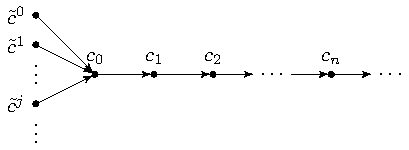
\includegraphics{final-f-infinite-local.pdf}
	\caption{Graphical representation of the ``final'' $f$}
	\label{fig:uai:final-f-sketch}
\end{figure*}

The main idea is to pick a suitable $f$ in $F$ and define the sequence as the iterates $c_{n+1} = f(c_n)$. This function is sketched in Figure~\ref{fig:uai:final-f-sketch}.
The initial set of elements $\tilde{c}^j$ mapped to $c_0$ is required to apply Lemma~\ref{lmm:uai:f-non-repr-pair} to all pairs $\{ \tilde{c}^j, c_n \}$ and get that $c_{n+1} = f(c_n)$ is representable, since $f(\tilde{c}^j) = c_0 \in R$.
The difficulty in realizing this idea is that we do not have enough information on the sequence to pick the right function $f$ at the beginning, so we bring along a list of candidate functions that all coincide on a prefix of the sequence. At step $n$, we pick a new element of the sequence among the possible images of $c_{n-1}$ through all candidate $f$ we have at that point and discard all those functions that cannot match the choice.
Actually, instead of directly considering functions, we represent them with elements $\tilde{c}$ of $C$. Each one represents a function $f_{\tilde{c}}$ that satisfies $f_{\tilde{c}}(\tilde{c}) = c_0$. Note that this can be done for ``enough'' (that is, infinitely many) $\tilde{c}$ because of the high surjectivity hypothesis. We call $E_n$ the set of element $\tilde{c}$ that represent functions that are ``valid'' for the prefix up to $n$, i.e., they map $c_{i}$ to $c_{i+1}$ for $0 \le i \le n - 1$. The core of the proof is an induction that proves that $E_n$ always contains infinitely many elements and that the newly chosen $c_n$ is different from all the previous ones.
\begin{theorem}\label{th:uai:non-empt-res-local}
	Let $F$ be a highly surjective function family from $C$ to itself such that all functions $f \in F$ are either injective or acyclic.
	Assume also that $R\neq \emptyset$. Then there is at least one function $f \in F$ that is not non-emptying in $A$.
\end{theorem}

\begin{remark}
	In the previous section, we developed an ad hoc proof for the family of sums over integers in Proposition~\ref{prop:uai:ne-sum-nonexsistence-inf}, but the same result can also be obtained as an application of Theorem~\ref{th:uai:non-empt-res-local}: if $C = \setZ$ and $F = \{ \lambda x. x + n \svert n \in \setZ \}$, the family is highly surjective (actually $P_F(c) = \setZ$ for all $c$) and all these functions are injective, so it meets the hypotheses of the theorem.
	However, it is interesting to note that the proof of Theorem~\ref{th:uai:non-empt-res-local} is not a generalization of the proof of Proposition~\ref{prop:uai:ne-sum-nonexsistence-inf}. Here we iterate a single $f$ to build the entire sequence, while in the previous one we change the function every time, mapping the non representable $\tilde{n}$ to the newly found representable $n_0 + t d$ to get that the image of $n_0$ through that function is representable too, as sketched in Figure \ref{fig:uai:ne-sum-inf-sketch}.
	\begin{figure*}[ht]
		\centering
		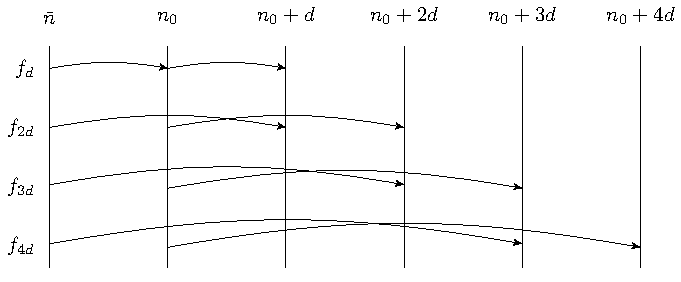
\includegraphics{proof-sum-infinite.pdf}
		\caption{Graphical representation of the proof of Proposition~\ref{prop:uai:ne-sum-nonexsistence-inf}}
		\label{fig:uai:ne-sum-inf-sketch}
	\end{figure*}
\end{remark}

Another example are rational or real numbers, with sums or products.
\begin{example}
	Take $C = \mathbb{Q} \setminus \{ 0 \}$ and $F = \{ \lambda x. x \cdot q \svert q \in \mathbb{Q} \setminus \{ 0 \} \}$.
	The family is highly surjective since $P_F(c) = \mathbb{Q} \setminus \{ 0 \}$ for all $c$, and all these functions are invertible, hence injective.
\end{example}
A possibly more interesting example of application are floating-point numbers as described by the IEEE Standard.
\begin{example}\label{ex:uai:fp-numbers-local}
	Take $C = \mathcal{F} \setminus \{ 0 \}$ the set of non-zero floating-point numbers that can be represented with a fixed number of significant digits, say $t$ bits, but with an arbitrary precision exponent. We choose infinite precision exponents but a finite number of significant digits to have an infinite domain, as required by the theorem, but also to preserve characteristics of floating-point arithmetic.

	Let $\cdot$ and $\odot$ denote respectively real product and its floating-point approximation, and consider the function family $F = \{ \lambda x . x \odot y \svert y \in C \}$. The function family is highly surjective, e.g., considering that all numbers with the same significant digits as a floating-point $x$ but different exponent can be mapped into $x$ by multiplying them by $2$ to the power of the difference of exponents.
	For the second condition, if $y = \pm 1$ we have that the function $\lambda x. x \odot y$ is invertible, hence injective. Otherwise, assume without loss of generality that $y > 1$ (other cases are analogous), and by contradiction assume it has a cycle $f^{n}(x_0) = x_0$. By monotonicity of $\odot$ we have 	$f(x) = x \odot y \ge x \odot 1 = x$, hence $x_0 \le f(x_0) \le f^2(x_0) \le \dots \le f^n(x_0) = x_0$ so all the elements of the cycle are equal, and in particular $f(x_0) = x_0$. However, if $y \neq 1$, the product $x \odot y$ is never equal to $x$, that is a contradiction. Hence the function is acyclic.
	This means $F$ meets the hypotheses of Theorem~\ref{th:uai:non-empt-res-local}, hence no abstract domain on floating-point numbers can be non-emptying for all multiplications.
\end{example}

\subsection{Global requirements for impossibility}
The second set of conditions we propose is ``global'', in the sense that it requires the family $F$ to satisfy a property as a whole.

The proof of this theorem starts from the infinite set $P_F(c_0)$ and, using the hypotheses that some sets are finite, propagates its infiniteness down to $R$, yielding a contradiction with Lemma~\ref{lmm:uai:R-S-bound-integer-inf}, stating that $R$ is finite.
\begin{theorem}\label{th:uai:non-empt-res-global}
	Let $F$ be a highly surjective family of functions  from $C$ to itself such that
	\begin{enumerate}
		\item for all pair of elements $c, d \in C$, the set $\{ f \in F \mid f(d) = c \}$ is finite;
		\item for all pair of an element $c \in C$ and a function $f \in F$, the set $\{ d \in C \mid f(d) = c \}$ is finite.
	\end{enumerate}
	Assume also that $R$ is not empty. Then there is at least one function $f \in F$ that is not non-emptying in $A$.
\end{theorem}

\begin{remark}
	Again, Theorem~\ref{th:uai:non-empt-res-global} can be used to prove Proposition~\ref{prop:uai:ne-sum-nonexsistence-inf}, but the proofs are different.
	The former starts from the infinite set $P_F(c_0) \setminus R(c_0)$ of preimages $\tilde{c}$ of $c_0$ that are not representable with it. This yields an infinite list of pairs $\{ \tilde{c}, c_0 \}$ to apply Lemma~\ref{lmm:uai:f-non-repr-pair}: for any such pair, since $\tilde{c}$ is in $P_F(c_0)$, we get a function $f_{\tilde{c}}$ such that $f_{\tilde{c}}(\tilde{c}) = c_0 \in R$, so that $f_{\tilde{c}}(c_0) \in R$, too. The proof then exploits the remaining hypotheses to prove that there are infinitely many distinct $f_{\tilde{c}}(c_0)$.
	The proof of the latter relies on multiple functions to apply Lemma~\ref{lmm:uai:f-non-repr-pair}, but it always uses the same pair $\{ \bar{n}, n_0 \}$: at every step, it finds a function that maps $\bar{n}$ to the representable element found at the previous step.
\end{remark}

Similarly to Theorem~\ref{th:uai:non-empt-res-local}, this result can be used to prove the impossibility of building an under-approximation abstract domain for floating-point numbers.
\begin{example}\label{ex:uai:fp-numbers-global}
	Take $C = \mathcal{F} \setminus \{ 0 \}$ the set of non-zero floating-point numbers with $t$ bits significands and arbitrary precision exponents, and $F = \{ \lambda x . x \odot z \svert z \in \mathcal{F} \setminus \{ 0 \} \}$.
	As observed in Example~\ref{ex:uai:fp-numbers-local} this family is highly surjective.
	Fixed now two floating-point numbers $x, y$, and letting $\macheps$ be the machine precision of floating-point arithmetic, we have that $y = x \odot z$ only if
	\[
	\left\lvert \frac{y - (x \cdot z)}{x \cdot z} \right\rvert < \macheps
	\]
	that is
	\[
	\left\lvert\frac{y}{x}\right\rvert \frac{1}{1+\macheps} < \abs{z} < \left\lvert\frac{y}{x}\right\rvert \frac{1}{1-\macheps}
	\]
	This is a bounded interval since $x \neq 0$, and hence contains only a finite amount of floating-point numbers. This in turn means that, fixed $x$ and $y$, there is only a finite amount of functions of the form $\lambda x. x \odot z$ such that $f(x) = y$.
	Analogously, fixed a floating-point $y$ and a function $f(x) = x \odot z$, we have that $y = f(x)$ only if $\abs{x}$ belong to a bounded interval, that contains a finite amount of floating-point numbers. So, fixed $y$ and a function $f = \lambda x . x \odot z$, only a finite number of $x$ satisfies $f(x) = y$.
	So, through Theorem~\ref{th:uai:non-empt-res-global} above, we proved again that no abstract domain on floating-point numbers can be non-emptying for all multiplications.
\end{example}

We point out once more that the only hypothesis on the abstract domain is about its size for both theorems in this section. For instance, our result applies to any under-approximation predicate abstraction domain~\cite{GS97}. Such a domain is defined by a (finite) list of predicates, each one representing the set of states satisfying the predicate, and an abstract state is a subset of predicates. By duality with respect to over-approximation, the concretization of such a set is the \emph{union} of the states described by each predicate. Analogously, the abstraction of a set of concrete states $S$ is the set of predicates which are \emph{entirely contained} in $S$. Note that this interpretation is consistent with the use of under-approximations in Incorrectness Logic: the difference is that the logic can use any under-approximation formula, while predicate abstraction is constrained to use just a finite set of predicates, fixed beforehand.

\subsection{On the necessity of high surjectivity}\label{sec:uai:high-surjective}
Both sets of conditions we proposed in this section require the function family to be highly surjective. This turns out to be necessary to prove that no under-approximation abstract domain exists, as we show in this section.

\begin{prop}\label{prop:uai:existence-base}
	For any fixed family $F$ of functions from $C$ to itself that is not highly surjective, there exists an abstract domain $A_F$ for $\pow(C)$ such that:
	\begin{itemize}
		\item $A_F$ is finite, and
		\item all functions $f \in F$ are non-emptying in $A_F$.
	\end{itemize}
\end{prop}

Notably, the above proof is constructive. We present an example of such domain construction below.
\begin{example}\label{ex:uai:construction-ne-domain-base}
	Fix the pair of functions $f(x) = x - 1$ and $g(x) = x - 2$ on $\setZ$. The family $F = \{ f, g \}$ is not highly surjective, so we build an under-approximation abstract domain for which these functions are non-emptying.
	First, take an integer $n_0$ such that $P_F(n_0)$ (computed with respect to $F$) is finite. With this $F$, any integer is a suitable candidate, so let us fix $n_0 = 0$.

	The set of preimages of $0$ is $P_F(0) = \{ 1, 2 \}$. We define the abstract domain $A_F$ as
	\[
	A_F = \{ \emptyset \} \cup \left\lbrace X \cup \{ 0 \} \svert X \subseteq P_F(0) \right\rbrace = \{ \emptyset, \{ 0 \}, \{ 0, 1 \}, \{ 0, 2 \}, \{ 0, 1, 2 \} \} .
	\]
	In this abstract domain, a set is abstracted to $\emptyset$ if and only if it does not contain $0$ since all elements of $A_F$ but $\emptyset$ contains $0$ and the abstraction of a set $S$ must be a subset of $S$.

	To check that $f$ is non-emptying in $A_F$, fix a set $S \subseteq \setZ$. If $\alpha(S) = \emptyset$ the non-emptying condition is vacuously true, so assume this is not the case, or, equivalently, that $0 \in S$. Analogously, if $\alpha(f(S)) = \emptyset$ the condition is true, so assume $0 \in f(S)$ or, equivalently, $1 \in S$. Using these two assumptions we get
	\begin{align*}
		f^{A}(\alpha(S)) & = \alpha(f(\alpha(S)))                  & [\text{def. of }f^{A}]                             \\
		                 & \supseteq \alpha(f(\alpha(\{ 0, 1 \}))) & [\alpha, f \text{ monotone}, S \supseteq \{0, 1\}] \\
		                 & = \alpha(f(\{ 0, 1 \}))                 & [\alpha(\{ 0, 1 \}) = \{ 0, 1 \}]                  \\
		                 & = \alpha(\{ -1, 0 \}) = \{ 0 \}         & [\text{def. of } f \text{ and } \alpha]
	\end{align*}
	The check for $g$ is analogous.
\end{example}
Even though this proposition defines an under-approximation abstract domain, it should not be interpreted as a positive result since the resulting domain is almost a power set and hence too large to be feasible in practice. Instead, the proposition should be regarded as a way to show that one of the hypotheses required in the previous theorems is tight and cannot be weakened. Particularly, since these kinds of results require high surjectivity, they are ill-suited when the focus is on a single function.

This proposition can be generalized to consider sets $S \subseteq C$ whose preimages are finite, but a little care is needed when lifting the definition of preimages to sets of values: a preimage is a set for which there exists a function that maps it to $S$, not the union of the preimages of elements in $S$. Formally, we let:
\[
P_F(S) = \{ T \subseteq C \svert \exists f \in F.~ f(T) = S \} .
\]
Using this definition, we can now easily generalize Proposition~\ref{prop:uai:existence-base}:
\begin{prop}\label{prop:uai:existence-finite-backward}
	Let $F$ be a family of functions from $C$ in itself, and assume there is a set $S_0 \subseteq C$ such that $P_F(S_0)$ is finite. Then there exists a finite abstract domain $A_F$ for $\pow(C)$ such that all functions $f \in F$ are non-emptying in $A_F$.
\end{prop}
This proposition may also be applied to the concrete domain of finite lists to show that a natural function family to consider cannot be used to prove non existence of under-approximation domains using non-emptying functions.
\begin{example}\label{ex:uai:construction-ne-domain-backward}
	Fix the concrete domain $C$ as the set of all lists of finite length over a finite, non-empty alphabet $\Gamma$, i.e. $C = \Gamma^{*}$.
	For $\alpha \in \Gamma^*$ a finite string, let
	\[
	\concat_{\alpha}(\beta) = \alpha \beta
	\]
	be the function that prefixes its argument by the string $\alpha$.
	The family
	\[
	F = \{ \concat_{\alpha} \svert \alpha \in \Gamma^* \}
	\]
	is not highly surjective, because fixed a string $\gamma$ only its suffixes can be mapped into  $\gamma$ by a function in $F$, and they are a finite amount. Hence we can define an under-approximation abstract domain for which all these functions are non-emptying by means of Proposition~\ref{prop:uai:existence-finite-backward}.
	Such domains are defined with a construction similar to that of Example~\ref{ex:uai:construction-ne-domain-base}, and in particular, if $\epsilon$ is the empty list, considering the set $S_0 = \{ \epsilon \}$ whose preimage is only $S_0$ itself, the construction yields
	\[
	A_F = \{ \emptyset, \{ \epsilon \} \} .
	\]
	It is easy to check that all functions $\concat_{\alpha}$ are non-emptying in this abstract domain.
\end{example}

The previous proposition focuses on preimages, stating that if there is a concrete element that has a finite amount of preimages then it is possible to define an under-approximation domain. A natural dual of this proposition can be formulated in terms of images.
For a subset $S \subseteq C$, the set of its images is defined as follows:
\[
I_F(S) = \{ f(S) \svert f \in F \} .
\]
This definition is exactly dual to that of preimages and can be used to formulate a similar result.
\begin{prop}\label{prop:uai:existence-finite-forward}
	Let $F$ be a family of total functions (ie. if $S \neq \emptyset$ then $f(S) \neq \emptyset$) from $\pow(C)$ in itself, and assume there is a non-empty set $S_0 \subseteq C$ such that $I_F(S_0)$ is finite. Then there exists a finite abstract domain $A_F$ such that all functions $f \in F$ are non-emptying in $A_F$.
\end{prop}
Even though Proposition~\ref{prop:uai:existence-finite-forward} introduces the technical hypothesis that all $f \in F$ are total, we don't believe this condition to be very restrictive in practice. Our results are applicable when $F$ is a family of basic transfer functions; in programming languages, non-termination is often due to control-flow constructs, while assignments and guards are usually total.
As an immediate application of the proposition that exploits images instead of pre-images, we consider lists again, and rule out another natural function family.
\begin{example}\label{ex:uai:construction-ne-domain-forward}
	Fix again $C = \Gamma^{*}$, and consider all functions of the form $\dropp_n : \Gamma^* \rightarrow \Gamma^*$ that, taken a list, drop its first $n$ elements and return the resulting list. If the input list is shorter than $n$, the output of $\dropp_n$ is the empty list $\epsilon$.
	The function family
	\[
	F = \{ \dropp_n \svert n \in \setN \}
	\]
	is highly surjective since, for any fixed list $\alpha \in \Gamma^*$ and any $n$, we can prefix $\alpha$ by $n$ arbitrary characters, and map this extended list back to $\alpha$ via $\dropp_n$.
	However, images through this function family are finite:
	\[
	I_F(\alpha) = \{ \dropp_n(\alpha) \svert n \in \setN \}
	\]
	is finite because $I_F(\alpha)$ coincides with the set of all tails of $\alpha$. By Proposition~\ref{prop:uai:existence-finite-forward} we can define an under-approximation abstract domain such that all functions $\dropp_n$ are non-emptying. Again, these domains are constructed from sets $S_0$ with a finite amount of images, and considering $S_0 = \{ \epsilon \}$, that satisfies $I_F(S_0) = \{ \epsilon \}$, we get
	\[
	A_F = \{ \emptyset, \{ \epsilon \} \} .
	\]
	It can be easily checked that all functions $\dropp_n$ are non-emptying in $A_F$.
\end{example}

These last two propositions consider opposite situations in which it is possible to define an under-approximation domain: the former requires to be able to go backward using $F$ in infinitely many ways, while the latter to go forward. This often is not the case in the presence of ``boundaries'' in the concrete domain, which are points with respect to which functions tend to walk either up or away. For instance, $\epsilon$ is such a point with finite lists because $\concat$ functions go away from it while $\dropp$ functions move towards it.
Another example of such a boundary is $0$ in the domain of integers $\setZ$ for multiplications and (rounded) divisions: the former increase absolute value, moving away from $0$ (even though $0$ itself is never a preimage), while the latter decrease it.
Also considering a function family made of both kinds of functions does not work: a slight adaptation of the constructions for the two propositions above shows that, if $F$ can be partitioned into two subfamilies, each satisfying the hypothesis of one of the two propositions, then there exists an under-approximation abstract domain. An example of this is in the set of finite lists, taking as $F$ both $\concat$ and $\dropp$ functions. The construction then yields exactly $A_F = \{ \emptyset, \{ \epsilon \} \}$, for which all these functions are non-emptying, as shown in Examples~\ref{ex:uai:construction-ne-domain-backward} and \ref{ex:uai:construction-ne-domain-forward}.
In light of these observations, to apply the definition of non-emptying function in an effective way for proving the non existence of abstract domains, for all possible boundaries there is the need for a function that can both enter and exit it. This happens for integers since there is no boundary, but does not for finite lists, with $\{ \epsilon \}$ being often either a sink or a source for many functions on lists.

\section{General finite concrete domains}\label{sec:uai:finite}
The discussion of Section~\ref{sec:uai:infinite} requires $C$ to be infinite. While this is a common simplification, since concrete domains have usually a very big size, an interesting and important question is whether our findings can be extended to the case of finite concrete domains.
However, we believe that the two Theorems~\ref{th:uai:non-empt-res-local} and \ref{th:uai:non-empt-res-global} cannot be straightforwardly adapted to the finite setting.

%For both these results, the proof of non existence of the abstract domain was carried out by showing the existence of infinitely many representable elements (defining an infinite sequence in the local result Theorem~\ref{th:uai:non-empt-res-local}, extracting a fraction of the infinite $P_F(c_0)$ in the global Theorem~\ref{th:uai:non-empt-res-global}), against Lemma~\ref{lmm:uai:R-S-bound-integer-inf}. For a finite $C$, if $N = \abs{C}$, one possibility would be to resort to Lemma~\ref{lmm:uai:R-S-bound-integer-fin} to show that $\abs{R} = O(\log(N))$ and get the contradiction by proving the existence of $\omega(\log(N))$ representable elements. Unfortunately, the same and similar constructions do not yield the desired bound: when $C$ is infinite we exploited the fact that finite combinations of finite numbers are also finite, while for finite $C$ we should require that arbitrary combinations of logarithmic factors are $O(N)$, which is not the case.
For both results, the proof showed the existence of infinitely many representable elements, contradicting Lemma~\ref{lmm:uai:R-S-bound-integer-inf}. For a finite $C$, if $N = \abs{C}$, one possibility would be to resort to Lemma~\ref{lmm:uai:R-S-bound-integer-fin} to show that $\abs{R} = O(\log(N))$ and get the contradiction by proving the existence of $\omega(\log(N))$ representable elements (we recall that $f(n) = \omega(g(n))$ if and only if $\lim_{n \rightarrow +\infty} \left( {f(n)} / {g(n)} \right) = +\infty$, which intuitively means that $f$ asymptotically dominates $g$). Unfortunately, similar constructions do not yield the desired bound: when $C$ is infinite we exploited the fact that finite combinations of finite numbers are also finite, while for finite $C$ we should require that arbitrary combinations of logarithmic factors are $O(N)$, which is not true.

The definition of highly surjective family itself is not easy to translate. The construction of Proposition~\ref{prop:uai:existence-base} on a finite $C$ yields an abstract domain with the needed features already when $\abs{P_F(c)} = O(\log(N))$. However, to carry out proofs along the lines of Theorems~\ref{th:uai:non-empt-res-local} and~\ref{th:uai:non-empt-res-global} we would need stronger hypothesis than just $\abs{P_F(c)} = \omega(\log(N))$, possibly up to $\abs{P_F(c)} = \Theta(N)$.

Even with these theoretical considerations against finite counterparts of Theorems~\ref{th:uai:non-empt-res-local} and~\ref{th:uai:non-empt-res-global}, we have been able to carry out the proof for the special case of the finite domain $C = [-N, N]$ of integers (Proposition~\ref{prop:uai:ne-sum-nonexsistence-fin}). Our result exploits the precise structure of both the given concrete domain and function family, particularly two key points.
First, functions produce elements that are not ``too far away'' with respect to the size of the domain (i.e., $n_{i+1} - n_{i} = O(\log(N))$), and this allows to prove that there are enough distinct representable elements.
Second, the domain is circular and hence has no boundaries. If the domain had them, we could have applied results such as Example~\ref{ex:uai:construction-ne-domain-backward} or Proposition~\ref{prop:uai:existence-finite-forward}. This was not the case for integers because additions overflow, so the domain has no boundaries near $-N$ and $N$.

Building on the above discussion, we present a version of the global condition for finite concrete domains. To overcome the limitation of boundaries, we explicitly constrain the initial representable element $c_0$, writing hypotheses around it. Such hypotheses imply that $c_0$ is ``far enough'' from the boundaries of the domain (if any).
Conditions (1-2) of the next theorem correspond to those of the infinite version (Theorem~\ref{th:uai:non-empt-res-global}) rewritten with $c_0$ in mind. The relation between the two bound functions $k_1$ and $k_2$ and the number of preimages of $c_0$ corresponds to the high surjectivity hypothesis. It only constrains the value $c_0$ because this is the representable value from which the proof begins.

As we did in the specific case of the integer domain $[-N; N]$, we assume the size of $A$ to be polynomial in $N$ (Assumption~\ref{assump:uai:size-A-finite-integers}). To say this formally, as we did for finite integers (cfr. Section~\ref{sec:uai:integers-finite}), we consider a sequence $C_N$ of sets of concrete values with size $O(N)$. In the specific instance of integers, such sets were the intervals $[-N; N]$; in general, we require that $C_{N-1} \subseteq C_N$ for all $N$. This inclusion formalizes the intuition that all the $C_N$ are the ``same'' concrete domain instantiated for different sizes.
We also assume to have an abstract domain $A_N$ for each concrete domain $\pow(C_N)$ such that $\abs{A_N} = O(\text{poly}(N))$. As before, we write $R_N$ for $R_{A_N}$, and we remark that Lemma~\ref{lmm:uai:R-S-bound-integer-fin} holds.

\begin{theorem}\label{th:uai:non-empt-res-finite-global}
	Assume $\abs{C_N} = O(N)$, and let $\ugi{\pow(C_N)}{\alpha_N}{A_N}$ be a UGI for all $N$.
	Assume there exists a number $N_1$ and a value $c_0 \in C_{N_1}$ such that, for all $N > N_1$, $c_0$ is representable in $A_N$ (i.e., $c_0 \in R_{N}$).
	Given  two functions $k_1, k_2 : \setN \rightarrow \setN_{>0}$, for any $N$
	let $F_N$ be a family of functions from $C_N$ to itself such that:
	\begin{enumerate}
		\item for all elements $d \in C_N$, $\abs{\{f \in F_N \mid f(c_0) = d \}} \leq k_1(N)$;
		\item for all functions $f \in F_N$, $\abs{\{d \in C_N \mid f(d) = c_0\}} \leq k_2(N)$.
	\end{enumerate}
	Lastly, assume that $\abs{P_{F_N}(c_0)} = \omega(\log(N) \cdot k_1(N) \cdot k_2(N))$.\\
	Then, there exists $N_0$ such that, for all $N > N_0$, it is not possible that all $f \in F_N$ are non-emptying in $A_N$.
\end{theorem}

A straightforward corollary is that, whenever we can verify the hypotheses for all values in $C$, there is no under-approximation domain with a representable element. This is for instance the case for integers and sums, so we recover Proposition~\ref{prop:uai:ne-sum-nonexsistence-fin}:
\begin{example}
	Let $C_N = [-N, N]$ and
	\[
	F_N = \{ \lambda x. x + n (\text{modulo } 2N+1) \svert n \in [-N, N] \} .
	\]

	Fixed any $n_0 \in [-N, N]$, it is easy to check that $P_F(n_0) = [-N, N]$ and $k_1(N) = k_2(N) = 1$. The condition
	\[
	\abs{P_F(n_0)} = \omega(\log(2N + 1) \cdot k_1(2N + 1) \cdot k_2(2N + 1))
	\]
	thus reduces to
	\[
	2N + 1 = \omega(\log(N))
	\]
	that is true. Hence there is no under-approximation abstract domain for integers with at least one integer $n_0$ representable and that makes all sums non-emptying.
\end{example}
The example of integers has the nice property of not having boundaries, but this is seldom the case. For instance, consider floating point numbers: they overflow and underflow to special values, hence they do have boundaries. Nevertheless, if we pick a suitable initial element $c_0$ we can still apply the theorem above.

\begin{example}
	Consider the finite set of non-zero floating-point numbers $C = \mathcal{F} \setminus \{ 0 \}$ with $t$ bits significand, one bit sign and $e$ bit exponents.
	Consider the function family $F = \{ \lambda x . x \odot z \svert z \in \mathcal{F} \setminus \{ 0 \} \}$ of floating-point multiplications, where $\odot$ denotes the floating-point approximation of real product.

	As shown in Example~\ref{ex:uai:fp-numbers-global}, fixed two floating-point numbers $x, y$, we have that $y = f(x) = x \odot z$ only if
	\[
	\abs{z} \in \left[ \left\lvert\frac{y}{x}\right\rvert \frac{1}{1+\macheps}, \left\lvert\frac{y}{x}\right\rvert \frac{1}{1-\macheps} \right] .
	\]
	If $\macheps \le 1 / 2$ this is entirely contained in the interval
	\[
	\left[ \left\lvert\frac{y}{x}\right\rvert (1 - 2 \macheps), \left\lvert\frac{y}{x}\right\rvert (1 + 2 \macheps) \right] \text{.}
	\]
	It can be shown that, if $\macheps < 1 / 2$, the quantity of floating point numbers in that interval is bounded by a constant $c$ that does not depend on $x$ and $y$.\footnote{For instance, this can be proved for $c = 17$.}
	Analogously, fixed $y$ and $z$ there are at most $c$ floating point numbers $x$ such that $y = f(x) = x \odot z$.

	With these two bounds, if $x_0$ has enough preimages we can verify the last hypothesis of the theorem: letting $N = \abs{C}$
	\[
	\abs{P_F(x_0)} = \omega(\log(N) \cdot k_1(N) \cdot k_2(N)) = \omega(\log(N) \cdot c \cdot c) = \omega(\log(N)) .
	\]
	For instance $x_0 = 1$ satisfies this condition (more than half of all floating-point numbers have a floating-point inverse, hence $\abs{P_F(x_0)} \ge N / 2 = \Theta(N)$) but there are many other points satisfying it.
	By mean of Theorem~\ref{th:uai:non-empt-res-finite-global}, no under-approximation abstract domain is non-emptying for all multiplications whenever one of these points is representable.
\end{example}

\section{Summary}
In this chapter, we pointed out some asymmetries between over and under-approximation in Abstract Interpretation, and why those are an obstacle to the design of abstract domains for program analysis via under-approximation Galois connections. The key observation is that the duality between under and over-approximation is broken by the fact that in program analysis over and under-approximations have to be applied to the same transfer functions. The handling of divergence in the abstract domain poses another critical issue.

Building on those ideas, we proposed the novel definition of \emph{non-emptying function} and studied how it plays a crucial role in proving the non-existence of general, useful under-approximation based abstract domains. Indeed, our results prove that an analysis based on such domains will very often answer $\bot$ (representing either absence of information or divergence) for programs that require repeated applications of non-emptying functions. This is a big limitation since recovery from $\bot$ in an under-approximation is not as easy as recovering from $\top$ in an over-approximation: we can say that it is quite impossible.
We applied our general results to several concrete domains to conclude that, under some mild assumptions, there are no useful under-approximation abstract domains for program analysis. Then, to show that one of the hypotheses in our result is tight, we proposed a construction to craft an under-approximation abstract domain whenever such a hypothesis is not met.

To summarize, our results hint at the difficulty of designing under-approximation abstract domains. This suggest that it is better to resort to other under-approximation techniques to combine with over-approximation ones, including usual over-approximation abstract interpretation domains. Therefore, in the next chapter we study logical frameworks for under-approximation.

% !TEX root = ../phd-thesis.tex

\chapter{A comparison of program logics}\label{ch:sil}
In this chapter, we consider three known triple-based program logics, namely Hoare Logic (HL), Incorrectness Logic (IL) and Necessary Conditions (NC). We characterize their validity conditions in term of over or under-approximation of forward and backward semantics. First, this allows us to identify the absence of one combination, and thus to define a new program logic, called Sufficient Incorrectness Logic (SIL), for it. Second, this guides a thorough comparison of the four validity conditions, highlighting analogies and differences between over and under-approximation approaches.

The content of this chapter is based on~\cite{ABGL24}.

\section{Taxonomy}
\begin{figure}[t]
	\centering

	\begin{tabular}{@{\quad}c@{\quad}|@{\quad}rcr@{\quad}}
		       & \multicolumn{1}{c}{Forward}             &                                        & \multicolumn{1}{c}{Backward}                                 \\[3pt]
		\hline &                                         &                                        &                                                              \\[-5pt]
		Over   & HL: \quad $\fwsem{\regr} P \subseteq Q$ & $\xleftrightarrow{\qquad\simeq\qquad}$ & NC: \quad $\bwsem{\regr}Q \subseteq P$                       \\[5pt]
		Under  & IL: \quad $\fwsem{\regr}P \supseteq Q$  &                                        & \textcolor{ACMBlue}{SIL: \quad $\bwsem{\regr}Q \supseteq P$}
	\end{tabular}
	\caption{The taxonomy of validity conditions. Columns indicate if validity is based on forward or backward semantics and rows the verse of approximation. HL and NC are equivalent ($\simeq$). SIL is our new logic.}
	\label{fig:sil:taxonomy}
\end{figure}

As discussed in Sections~\ref{sec:bg:hl} and \ref{sec:bg:il}, the validity conditions of HL and IL are defined as over and under-approximation of the forward semantics $\fwsem{\cdot}$. However, other program logics cannot be naturally described in terms of $\fwsem{\cdot}$. To this end, we consider a backward semantics $\bwsem{\cdot}$ defined as the converse relation of the forward semantics,\footnote{Formally, if we consider a relation $\mathcal{R}$ between states defined as $\sigma \mathcal{R} \sigma'$ iff $\sigma' \in \fwsem{\regr} \sigma$, the backward semantics $\bwsem{\regr}$ defines the converse relation $\mathcal{R}^{-1}$} that is

\begin{equation}
	\bwsem{\regr} \sigma' \eqdef \{ \sigma \mid \sigma' \in \fwsem{\regr} \sigma \} \label{eq:sil:bwsem-definition}
\end{equation}

\noindent or, equivalently,

\begin{equation}
	\sigma \in \bwsem{\regr} \sigma' \iff \sigma' \in \fwsem{\regr} \sigma  \label{eq:sil:bwsem-sigma-sigma'}
\end{equation}

\noindent and we additively lift this definition to set of states by union.
Intuitively, the forward semantics $\fwsem{\regr} P$ denotes the set of all possible output states of $\regr$ when execution starts from a state in $P$ (and $\regr$ terminates).
Instead, the backward semantics $\bwsem{\regr} Q$ denotes the set of all input states that can lead to a state in $Q$.

The backward semantics can also be characterized compositionally, similarly to the forward one:

\begin{lemma}\label{lmm:sil:bwsem-calculus}
	For any regular commands $\regr,\regr_1,\regr_2\in \Reg$, the following equalities hold:
	\[
	\bwsem{\regr_1; \regr_2} = \bwsem{\regr_1} \circ \bwsem{\regr_2} \qquad\qquad
	\bwsem{\regr_1 \regplus \regr_2} = \bwsem{\regr_1} \cup \bwsem{\regr_2} \qquad\qquad
	\bwsem{{\regr^\kstar}} = \bigcup\limits_{n \ge 0} \bwsem{\regr}^n
	\]
\end{lemma}

Using $\bwsem{\cdot}$, we characterize NC with the validity condition $\bwsem{\regr} Q \subseteq P$.
To see why, assume $Q$ describes good final states. Then, $\bwsem{\regr} Q$ defines all states which can reach a good state. Since a precondition $\underline{P}$ is necessary for $Q$ if it contains every state which can reach a state in $Q$, $\underline{P}$ must contain at least all states in $\bwsem{\regr} Q$. More formally, for any initial state $\sigma \in \bwsem{\regr} Q$, there exist a $\sigma' \in \fwsem{\regr} \sigma$ such that $\sigma' \in Q$. This means that $\sigma$ has a trace in $\mathcal{T}(\sigma)$ (the one ending in $\sigma'$), so it must belong to any necessary precondition $\underline{P}$.

\begin{prop}[NC as backward over-approximation]\label{prop:sil:nc}
	Given a postcondition $Q$ for the program $\regr$, any possible necessary precondition $\underline{P}$ for $Q$ satisfies
	\[
	\bwsem{\regr} Q \subseteq \underline{P}
	\]
\end{prop}

Note that this is not a new understanding of NC (it was already hinted in the work that introduced them, and an analogous characterization appeared in~\cite[§6.3]{ZK22} in terms of weakest precondition), but the explicit use of the backward semantics in our contest enables a more streamlined comparison with other logics in Section~\ref{sec:sil:comparison}.

We organize the validity conditions of HL, IL and NC in the taxonomy in Figure~\ref{fig:sil:taxonomy}. We classify logics depending on (1) whether the condition is expressed in terms of forward or backward semantics and (2) whether it is an over or an under-approximation.
This naturally sparks the question on what does the backward under-approximation condition mean and whether a logic for it has been developed.

\paragraph{Backward under-approximation and Lisbon Triples}
At POPL'19 in Lisbon, D. Dreyer and R. Jung suggested that P. O'Hearn should look at bug-finding in terms of a logic for proving the presence of faults (as reported in~\cite{OHearn20,ZDS23}).
However, the proposed model of triples did not fit well with a key feature of Pulse, a bug-catching tool developed at Meta, namely its ability to drop the analysis of some program paths, for which IL provides a sound logical foundation instead.
The idea of such ``Lisbon'' triples is that \emph{for any initial state satisfying the pre, there exists some execution trace leading to a final state satisfying the post} and it can be dated back to Hoare's calculus of possible correctness~\cite{Hoare78}, even if no form of approximation was considered there.
Lisbon triples were then briefly discussed in~\cite[\S 5]{MOH21} and \cite[\S 3.2]{LRVBDO22} under the name \emph{backwards under-approximate triples}. They were also one of the motivations for OL~\cite{ZDS23}: OL recognized the importance of tracking the sources of errors and can encode Lisbon triples together with Hoare triples.
Backward under-approximation was also key for the development of a compositional non-termination analysis that has been integrated in Pulse~\cite{RVO24}, based on the observation that forward and backward under-approximation can be unified in a single logical framework by dropping the respective consequence rules.

Ideally, given an incorrectness specification, the goal of backward under-approximation would be to report to programmers all dangerous input states that lead to bugs.
However, all the above proposals are designed according to the forward semantics of programs and thus are best suited to infer postconditions starting from some given precondition. %: in general, their backward analysis may require the instantiation of their consequence rules with some ingenious guess.
To tackle this issue, we introduce Sufficient Incorrectness Logic (SIL) as a proof system for Lisbon triples with backward\hyp{}oriented rules.

Since in this chapter we deal with different kinds of program logics, a summary of the notation for the various triples is reported in Figure~\ref{fig:sil:notation-summary}.

\begin{figure}
	\centering
	\begin{tabular}{c|c@{\quad\enspace}c@{\quad\enspace}c@{\quad\enspace}c@{\quad\enspace}c}
		Logic                    &
		HL \cite{Hoare69}        &
		IL \cite{OHearn20}       &
		NC \cite{CCL11}          &
		OL \cite{ZDS23}          &
		SIL \cite{ABGL24}
		\\[2pt] \hline &&&&& \\[-10pt]
		Triples                  &
		$\hltriple{P}{\regr}{Q}$ &
		$\iltriple{P}{\regr}{Q}$ &
		$\nctriple{P}{\regr}{Q}$ &
		$\oltriple{P}{\regr}{Q}$ &
		$\siltriple{P}{\regr}{Q}$
	\end{tabular}
	\caption{Summary of the notation for different program logics}
	\label{fig:sil:notation-summary}
\end{figure}

\section{Sufficient Incorrectness Logic}\label{sec:sil:sil}

SIL is a backward\hyp{}oriented under\hyp{}approximation proof system for Lisbon triples that focuses on \emph{finding the sources of incorrectness rather than highlighting the presence of bugs}. Assuming the post $Q$ defines some class of errors, i.e., it is what we call an \emph{incorrectness specification}, a (valid) SIL triple $\siltriple{P}{\regr}{Q}$ means that ``\emph{all input states that satisfy $P$ have at least one execution of the program $\regr$ leading to a state that satisfies $Q$}''. For deterministic programs, SIL guarantees that a state satisfying the pre \emph{always} leads to an error. Instead, if $\regr$ is nondeterministic, SIL guarantees that there \emph{exists} an execution that leads to an error. Sufficient incorrectness preconditions are extremely valuable to programmers: by pointing out the sources of errors, they serve as a starting point to scope down debugging, fuzzing, and testing. Moreover, it is known that, contrary to IL and its extensions, backward under\hyp{}approximation can expose manifest errors \cite[§3.2]{LRVBDO22}: an error $Q$ is manifest iff the SIL triple $\siltriple{\true}{\regr}{Q}$ is valid. These are bugs that happen regardless of the context and it has been observed experimentally that are more likely to be fixed when reported~\cite[§5]{LRVBDO22}. Therefore, we study SIL to enhance program analysis frameworks with the ability to identify the source of incorrectness.

SIL goals include: (i)~defining a default deduction mechanism that starts from some specification of erroneous outcomes and traces the computation back to some initial states responsible for such errors; (ii)~exhibiting a minimal set of rules that are complete and correct for Lisbon triples; and (iii)~spelling out, a posteriori, a formalization and generalization of the backward analysis step performed by industrial grade analysis tools for security developed at Meta~\cite{DFLO19,MarianaTrench,Pysa}.
Those tools automatically find more than $50$\% of the security bugs in the Meta family of apps and many severe bugs~\cite[Fig.~5]{DFLO19}.

Roughly, the SIL triple
\[
\siltriple{P}{\regr}{Q}
\]
requires that all states in $P$ have at least one execution leading to a state in $Q$. More formally, for all $\sigma \in P$ there must exist a state $\sigma' \in Q$ such that $\sigma' \in \fwsem{\regr} \sigma$. Particularly, in the presence of nondeterminism states in $P$ are required to have one execution leading to $Q$, not necessarily all of them. Motivated by Figure~\ref{fig:sil:taxonomy}, we choose the validity condition
\[
\bwsem{\regr} Q \supseteq P. \tag{SIL}
\]
However, the two definition are equivalent:

\begin{prop}[Characterization of SIL validity]\label{prop:sil:sil-validity-characterization}
	For any $\regr \in \Reg$, $P, Q \subseteq \Sigma$
	\[
	\bwsem{\regr} Q \supseteq P \iff \forall \sigma \in P \sdot \exists \sigma' \in Q \sdot \sigma' \in \fwsem{\regr} \sigma
	\]
\end{prop}

A convenient way to exploit SIL is to assume that the analysis takes as input the incorrectness specification $Q$, i.e., the set of erroneous final states. Then, any valid SIL triple $\siltriple{P}{\regr}{Q}$ yields a precondition which surely captures erroneous executions. In this sense, $P$ gives a sufficient condition for incorrectness and motivates the name of SIL. This is dual to the interpretation of IL where, for a given precondition $P$, any IL triple $\iltriple{P}{\regr}{Q}$ yields a set $Q$ of final states which are for sure reachable, so that any error state in $Q$ is a true bug reachable from some input in $P$.

\subsection{Proof system}\label{sec:sil:sil-rules}

\begin{figure*}[t]
	\centering
	\begin{framed}
		\(
		\begin{array}{cc}
			\infer[\silrule{atom}]
			{\siltriple{\bwsem{\regc}Q}{\regc}{Q}}
			{}
			\quad                        &
			\infer[\silrule{cons}]
			{\siltriple{P}{\regr}{Q}}
			{P \subseteq P'              & \siltriple{P'}{\regr}{Q'}    & Q' \subseteq Q}
			\\[7.5pt]
			\infer[\silrule{seq}]
			{\siltriple{P}{\regr_1;\regr_2}{Q}}
			{\siltriple{P}{\regr_1}{R}   & \siltriple{R}{\regr_2}{Q}}
			\qquad                       &
			\infer[\silrule{choice}]
			{\siltriple{P_1 \cup P_2}{\regr_1 \regplus \regr_2}{Q}}
			{\siltriple{P_1}{\regr_1}{Q} & \siltriple{P_2}{\regr_2}{Q}}
			\\[7.5pt]
			\infer[\silrule{iter}]
			{\siltriple{\bigcup\limits_{n \ge 0} Q_n}{\regr^\kstar}{Q_0}}
			{\forall n \ge 0 \sdot \siltriple{Q_{n+1}}{\regr}{Q_n}}
		\end{array}
		\)\\
		\vspace{0.3em}
		\hrulefill \\
		\vspace{-2.5ex}\hrulefill
		\vspace{-0.2em}
		\begin{center}
			\small Additional rules
		\end{center}
		\(
		\begin{array}{cc}
			\infer[\silrule{empty}]
			{\siltriple{\emptyset}{\regr}{Q}}
			{}
			\qquad                       &
			\infer[\silrule{iter0}]
			{\siltriple{Q}{\regr^\kstar}{Q}}
			{}
			\\[7.5pt]
			\infer[\silrule{unroll}]
			{\siltriple{P}{\regr^\kstar}{Q}}
			{\siltriple{P}{\regr^\kstar; \regr}{Q}}
			\qquad                       &
			\infer[\silrule{disj}]
			{\siltriple{P_1 \cup P_2}{\regr}{Q_1 \cup Q_2}}
			{\siltriple{P_1}{\regr}{Q_1} & \siltriple{P_2}{\regr}{Q_2} }
		\end{array}
		\)
	\end{framed}
	\caption{Sufficient Incorrectness Logic}\label{fig:sil:sil-rules}
\end{figure*}

The inference rules for SIL are in Figure~\ref{fig:sil:sil-rules}. The top five rules form a minimal, sound and complete proof system. The additional rules are other valid rules that can ease program analysis and are discussed in Section~\ref{sec:sil:sil-rules-additional}.

Note that all the rules can be applied to an arbitrary post $Q$ to infer a corresponding pre, in the same way as all the rules of IL can be applied to an arbitrary pre $P$ to infer a corresponding post. This is a key feature of SIL proof system, which facilitates backward reasoning.

Atomic commands are handled by \silrule{atom}, which exploits the backward semantics and summarizes cases for \code{skip}, assignments and Boolean guards. In Section~\ref{sec:sil:rules-comparison} we discuss further the rule for assignment when pre and postconditions are formulae instead of sets of states.
The consequence rule allows to generalize a proof by weakening/strengthening the two conditions $P$ and $Q$ involved. It can readily be derived from the validity condition (SIL). Moreover, \silrule{cons} allows SIL to drop disjuncts in the pre, just as \ilrule{cons} allows IL do it in the post. This feature is crucial in both SIL and IL to increase scalability of tools.
Rule \silrule{seq} is standard: SIL triples are composed sequentially just like in all other logics.
Rule \silrule{choice} states that if all states in $P_1$ (resp. $P_2$) have an execution of $\regr_1$ (resp. $\regr_2$) ending in $Q$, they also have an execution of $\regr_1 \regplus \regr_2$ ending in $Q$ since the semantics of $\regr_1 \regplus \regr_2$ is a superset of that of $\regr_1$ (resp. $\regr_2$), cf. Figure~\ref{fig:bg:regcom-sem}. This rule is also reminiscent of the equation for conditionals in the calculus of possible correctness \cite{Hoare78}.
For iteration, for each $n \ge 0$ we find inductively the precondition $Q_n$ of executing $\regr$ exactly $n$ times. The precondition of the whole $\regr^{\kstar}$ is then the union of all the $Q_n$, as formalized by rule \silrule{iter}, which first appeared in \cite[§5]{MOH21}.

The SIL proof system is both correct and complete. Correctness can be proved by induction on the derivation tree of a triple. Intuitively, if the premises of a rule are valid, then its consequence is valid as well, as we briefly observed in above. To prove completeness, we rely on the fact that rules other than \silrule{cons} are exact, that is, if their premises satisfy the equality $\bwsem{\regr} Q = P$, their conclusion does as well. Using this, we prove the triple $\siltriple{\bwsem{\regr}Q}{\regr}{Q}$ for any $\regr$ and $Q$. We conclude using \silrule{cons} to get a proof of $\siltriple{P}{\regr}{Q}$ for any $P \subseteq \bwsem{\regr}Q$.

\begin{theorem}[SIL is sound and complete]\label{thm:sil:sil-sound-complete}
	A SIL triple is provable iff it is valid:
	\[
	\vdash\siltriple{P}{\regr}{Q} \iff \vDash\siltriple{P}{\regr}{Q}
	\]
\end{theorem}

\subsection{Additional rules for program analysis}\label{sec:sil:sil-rules-additional}
The topmost set of five rules in Figure~\ref{fig:sil:sil-rules} is deliberately minimal: if we remove any rule it is no longer complete. However, there are other valid rules, not derivable from those five, that can be useful in practice. Some of them are at the bottom of Figure~\ref{fig:sil:sil-rules}.

Rule \silrule{empty} is used to drop paths backward, just like IL can drop them forward (an analogous axiom $\iltriple{P}{\regr}{\emptyset}$ is valid for IL). Particularly, this allows to ignore one of the branches of \silrule{choice}, or to stop the backward iteration of \silrule{iter} without covering all the iterations. An example of such an application is the derived rule \silrule{iter0}, which corresponds to not entering the iteration at all. It can be derived from rules \silrule{iter} and \silrule{empty} by taking $Q_0 = Q$ and $Q_n = \emptyset$ for $n \ge 1$. It subsumes HL's rule \hlrule{iter}, which is based on loop invariants: those are a correct but not complete reasoning tool for under\hyp{}approximation~\cite{OHearn20}.
Rule \silrule{unroll} allows to unroll a loop once. Subsequent applications of this rule allow to simulate (backward) a finite number of iterations, and then rule \silrule{iter0} can be used to ignore the remaining ones. This is on par with IL ability to unroll a loop a finite number of times to find some post, for which analogous rules are valid~\cite{OHearn20,MOH21}.
Rule \silrule{disj} allows to split the analysis and join the results, just like HL and IL. However, while a corresponding rule \hlrule{conj} which perform intersection is sound for HL, it is unsound for both IL and SIL. We discuss this point further in Section~\ref{sec:sil:extremal-conditions}.

All four these additional rules are sound:
\begin{prop}[Soundness of additional SIL rules]\label{prop:sil:sil-additional-soundness}
	The additional SIL rules at the bottom of Figure~\ref{fig:sil:sil-rules} are sound, that is, triples provable in SIL extended with those rules are valid.
\end{prop}

\begin{example}\label{ex:sil:derivation}
	Let us consider the program ``loop0'' from~\cite[\S 6.1]{OHearn20}:

	\begin{minted}{C}
x := 0;
n := nondet();
while(n > 0) {
    x := x + n;
    n := nondet();
}
// assert(x != 2000000)
	\end{minted}

	We can translate it in the syntax of regular commands by letting
	\begin{align*}
		\regr_w         & \eqdef \code{(n > 0)?; x := x + n; n := nondet()}                         \\
		\mathsf{rloop0} & \eqdef \code{x := 0; n := nondet(); }(\regr_w)^{\kstar}; \code{(n <= 0)?}
	\end{align*}
	Final error states are those in $Q_{2M} \eqdef (x = 2 000 000)$.

	\begin{figure}[t]
		\centering
		\footnotesize
		\[
		\infer[]
		{(*)}
		{
			\infer[\silrule{seq}]{\siltriple{T_{2M}}{\regr_w^{\kstar}; \code{(n <= 0)?}}{Q_{2M}}}{
				\infer[\silrule{unroll}]{\siltriple{T_{2M}}{\regr_w^{\kstar}}{R_{2M}}}{
					\infer[\silrule{seq}]{\siltriple{T_{2M}}{\regr_w^{\kstar}; \regr_w}{R_{2M}}}{
						\infer[\silrule{iter0}]{\siltriple{T_{2M}}{\regr_w^{\kstar}}{T_{2M}}}{}
						&
						\infer{\siltriple{T_{2M}}{\regr_w}{R_{2M}}}{\vdots}
					}
				}
				&
				\infer[\silrule{atom}]{\siltriple{R_{2M}}{\code{(n <= 0)?}}{Q_{2M}}}{}
			}
		}
		\]

		\[
		\infer[\silrule{seq}]
		{\siltriple{\true}{\mathsf{rloop0}}{Q_{2M}}}
		{
			\infer[\silrule{seq}]{\siltriple{\true}{\code{x := 0; n := nondet()}}{T_{2M}}}{
				\infer[\silrule{atom}]{\siltriple{\true}{\code{x := 0}}{x \le 2000000}}{}
				&
				\infer[\silrule{atom}]{\siltriple{x \le 2000000}{\code{n := nondet()}}{T_{2M}}}{}
			}
			&
			(*)
		}
		\]
		\caption{Derivation of the SIL triple $\siltriple{\true}{\mathsf{rloop0}}{Q_{2M}}$ for Example~\ref{ex:sil:derivation}.}
		\label{fig:sil:example-derivation}
	\end{figure}

	To prove a triple for $\mathsf{rloop0}$, we have to perform at least one iteration, and we do so using \silrule{unroll}.
	We let $R_{2M} \eqdef (x = 2000000 \land n \le 0)$ and $T_{2M} \eqdef (x + n = 2000000 \land n > 0)$. It is straightforward to prove $\siltriple{T_{2M}}{\regr_w}{R_{2M}}$ via \silrule{seq} and \silrule{atom}. Given this triple, we can unroll the loop once and prove the same triple for $\regr_w^{\kstar}$, as shown by the combination of \silrule{unroll}, \silrule{seq} and \silrule{iter0} at the top-left of Figure~\ref{fig:sil:example-derivation}. This is a property of under-approximation: a nondeterministic number of iterations can be under-approximated by a single iteration \cite[\S 6.1]{OHearn20}.
	With this triple for the loop, we can prove for the whole program the triple $\siltriple{\true}{\mathsf{rloop0}}{Q_{2M}}$ using \silrule{seq} and \silrule{atom}. The full derivation is in Figure~\ref{fig:sil:example-derivation}.

	Differently than IL, this triple highlights that any initial state can lead to an error: instead of reporting the presence of a true bug, we can prove that this is a manifest error and produce an initial state which causes the bug.
\end{example}

\section{Relations among logics}\label{sec:sil:comparison}
We first follow the two-dimensional scheme in Figure~\ref{fig:sil:taxonomy} to carry out a duality-driven comparison among the four validity conditions. Then, we realize that analogies and differences between them can be studied along other axes to obtain interesting insights among the relations between over/under-approximation, forward/backward analysis, reachability/divergence, and others.

We named columns of Figure~\ref{fig:sil:taxonomy} based on which semantics (forward or backward) they use. However, there is not a unique way of fixing the over and under-approximation axes. For instance, it is possible to take the consequence rules as the approximation axis, naming IL and NC as under-approximation because you can always substitute $Q$ for one of its under-approximations $Q' \subseteq Q$. However, we chose to denote approximation depending on the ``target'' set, that is, $Q$ for forward and $P$ for backward semantics, respectively. We motivate this choice because it classifies both IL and SIL as under-approximation and they share the ability to drop program paths (e.g., by finite unrolling of loops).

\subsection{Pairwise comparison}
We first carry out a comparison of the logics two by two. We skip the pair HL and IL since it was already discussed when IL was introduced in \cite{OHearn20}.

\subsubsection{NC and IL}
Sufficient preconditions are properties that imply Dijkstra's $\wlp$: $\overline{P}$ is sufficient for a postcondition $Q$ if and only if $\overline{P} \subseteq \wlp[\regr](Q)$, which in turn is equivalent to validity of the HL triple $\hltriple{\overline{P}}{\regr}{Q}$. Necessary and sufficient preconditions are dual, and so are IL and HL. Moreover, NC and IL enjoy the same consequence rule: both can strengthen the post and weaken the pre. This double duality suggests a relation between NC and IL. However, the following example shows this is not the case.

\begin{example}\label{ex:sil:nc-and-il}
	Consider the nondeterministic program $\regr 42$ from Example~\ref{ex:bg:il-hl-comparison}, where $Q_{42} \eqdef (z = 42)$. For brevity, we let $Q'_{42} \eqdef (Q_{42} \land \text{odd}(y) \land \text{even}(x))$.
	From that Example we know that $\iltriple{z = 11}{\regr 42}{Q'_{42}}$ is valid in IL. However, we observe that the NC triple $\nctriple{z = 11}{\regr 42}{Q'_{42}}$ is not valid because, e.g., the state $[y \mapsto 1, z \mapsto 10]$ has an execution leading to $Q'_{42}$ but doesn't satisfy $z = 11$.
	Moreover, take for instance $\underline{P} \eqdef \text{odd}(y)$, which makes the NC triple $\nctriple{\underline{P}}{\regr 42}{Q'_{42}}$ valid (in any state \emph{not} satisfying $\underline{P}$ $y$ is even, is not changed by $\regr 42$ and should be odd to satisfy $Q'_{42}$). Then it is clear that $(z = 11) \notimplies \underline{P}$. This shows that not only IL triples do not yield NC triples, but also that in general there are NC preconditions which are not implied by IL preconditions.

	Conversely, consider $\lnot Q_{42} = (z \neq 42)$. While the NC triple $\nctriple{\true}{\regr 42}{\lnot Q_{42}}$ is valid, the IL triple $\iltriple{\true}{\regr 42}{\lnot Q_{42}}$ is not: for instance, the final state $[x \mapsto 11, y \mapsto 11, z \mapsto 11]$ is not reachable from any initial state. It follows that the IL triple $\iltriple{P}{\regr 42}{\lnot Q_{42}}$ is not valid for any $P$.
\end{example}

Given $\vDash \nctriple{\underline{P}}{\regr}{Q}$ and $\vDash \iltriple{P}{\regr}{Q}$, there always are states satisfying both $P$ and $\underline{P}$, i.e., $P \cap \underline{P} \neq \emptyset$. However, in general neither $P \subseteq \underline{P}$ nor $\underline{P} \subseteq P$. The difference between NC and IL becomes apparent when we spell out their validity conditions using quantifiers:
\begin{align*}
	\forall \sigma' \in Q \sdot \forall \sigma\in \bwsem{\regr}\sigma' \sdot\sigma\in P
	\tag{NC$_{\text{FOL}}$} \\
	\forall \sigma' \in Q \sdot \exists \sigma\in \bwsem{\regr}\sigma' \sdot \sigma \in P
	\tag{\ref{eq:bg:il-fol}}
\end{align*}
Initial states are universally quantified in (NC$_{\text{FOL}}$)---\emph{all} initial states with a good run must satisfy the precondition---but they are existentially quantified in (IL$_{\text{FOL}}$). We also note that, when $\regr$ is reversible (i.e., $\fwsem{\regr}$ is injective) any valid IL triple is also a valid NC triple.

\subsubsection{NC and HL}
It turns out that NC is strongly connected to weakest liberal preconditions and thus to HL.
Let $Q$ be a correctness postcondition: a finite trace is in $\mathcal{T}(\sigma)$ if its final state satisfies $Q$ and in $\mathcal{E}(\sigma)$ otherwise. In general, a necessary precondition has no relationship with $\wlp[\regr](Q)$. However, if we consider $\lnot Q$ instead of $Q$, we observe that ``erroneous" executions becomes those in $\mathcal{T}(\sigma)$ and ``correct" ones those in $\mathcal{E}(\sigma)$.
This means that $\mathcal{T}(\sigma) = \emptyset$ iff $\sigma \in \wlp[\regr](\lnot Q)$, from which we derive $\lnot \underline{P} \subseteq \wlp[\regr](\lnot Q)$ or, equivalently, $\lnot \wlp[\regr](\lnot Q) \subseteq \underline{P}$.

\begin{example}
	Consider again program $\regr 42$ from Example~\ref{ex:bg:il-hl-comparison} and the correctness specification $\lnot Q_{42} = (z\neq 42)$. We have that $\wlp[\regr 42](\lnot \lnot Q_{42}) = Q_{42}$, because if initially $z \neq 42$ then it is possible that $x$ is assigned an odd value and $z$ is not updated.
	Hence, a condition $P$ is implied by $\lnot \wlp[\regr](\lnot\lnot Q_{42}) = \lnot Q_{42}$ if and only if it is necessary. For instance, $(z \neq 42 \lor \text{odd}(y))$ is necessary but $(z > 42)$ is not.
\end{example}

The next bijection establishes the connection between (NC) and (HL): a necessary precondition is just the negation of a sufficient precondition for the negated post. This was also observed using weakest (liberal) preconditions in \cite[Theorem~5.4]{ZK22}.

\begin{prop}[Bijection between NC and HL]\label{prop:sil:fw-inclusion-negation-bw}
	For any  $\regr\in \Reg$ and $P, Q \subseteq \Sigma$:
	\[
	\fwsem{\regr} P \subseteq Q \Leftrightarrow \bwsem{\regr} (\lnot Q) \subseteq \lnot P \text{.}
	\]
\end{prop}

\subsubsection{SIL and IL}
Proposition~\ref{prop:sil:fw-inclusion-negation-bw} highlights an isomorphism between (HL) and (NC). By duality, this naturally sparks the question whether a similar connections between (IL) and (SIL) exists. The next example shows this is not the case.

\begin{example}\label{ex:sil:il-sil-incomparable}
	Since IL and SIL enjoy different consequence rules, neither of the two can imply the other with the same $P$ and $Q$. If we take negation into account, consider the program $\regr 1 \eqdef \code{x := 1}$.
	Both the SIL triple $\siltriple{x \ge 0}{\regr 1}{x = 1}$ and the IL triple $\iltriple{x \ge 0}{\regr 1}{x = 1}$ are valid. However, neither $\iltriple{x < 0}{\regr 1}{x \neq 1}$ nor $\siltriple{x < 0}{\regr 1}{x \neq 1}$ are valid.
	So neither (IL) implies negated (SIL) nor the other way around.
\end{example}

To gain some insights on why (SIL) and (IL) are not equivalent, we introduce the following concepts.

\begin{definition}
	Given a regular command $\regr$, we define the set of states that only diverges $D_{\regr}$ and the set of unreachable states $U_{\regr}$:
	\[
	D_{\regr} \eqdef \{ \sigma \mid \fwsem{\regr}\sigma = \emptyset \}
	\qquad
	U_{\regr} \eqdef \{ \sigma' \mid \sigma' \not\in\fwsem{\regr} \Sigma \} = \{ \sigma' \mid \bwsem{\regr}\sigma' = \emptyset \}.
	\]
\end{definition}

These two definition are dual when we reverse the execution direction: if we consider $\bwsem{\regr}$ instead of $\fwsem{\regr}$, the roles of $D$ and $U$ are swapped. This means that, in a sense, $U_{\regr}$ is the set of states which ``diverge" going backward.

\begin{lemma}\label{lmm:sil:CC-1-monotone}
	For any regular command $\regr \in \Reg$ and sets of states $P, Q \subseteq \Sigma$ it holds:
	\begin{enumerate}
		\item\label{lmm:sil:CC-1-monotone:1} $\bwsem{\regr} \fwsem{\regr} P \supseteq P \setminus D_{\regr}$;
		\item\label{lmm:sil:CC-1-monotone:2} $\fwsem{\regr} \bwsem{\regr} Q \supseteq Q \setminus U_{\regr}$.
	\end{enumerate}
\end{lemma}

This lemma highlights the asymmetry between over and under-approximation: the composition of a function with its inverse is increasing (but for non-terminating states).
This explains why (HL) and (NC) are related while (IL) and (SIL) are not: for over-approximation, $P \setminus D_{\regr} \subseteq \bwsem{\regr} \fwsem{\regr} P$ can be further exploited if we know $\fwsem{\regr} P \subseteq Q$ via (HL), but it cannot when $\fwsem{\regr} P \supseteq Q$ via (IL).

Lastly, while IL and SIL are not directly comparable, the preprint~\cite{RVO24} introduces a forward-oriented proof system with a core set of rules that are sound for both IL and SIL, therefore proving only triples that are valid for both. It also becomes complete for IL, resp. SIL, when augmented with the corresponding consequence rule.

\subsubsection{SIL and HL}
In general, HL and SIL are different, but they coincide whenever the program $\regr$ is deterministic and terminates for every input.

\begin{prop}\label{prop:sil:sil-hl-deterministic-terminating}
	For any $\regr\in \Reg$ and $P, Q \subseteq \Sigma$:
	\begin{itemize}
		\item if $\regr$ is deterministic, $\bwsem{\regr} Q \supseteq P \Rightarrow \fwsem{\regr} P \subseteq Q$
		\item if $\regr$ is terminating, $\fwsem{\regr} P \subseteq Q \Rightarrow \bwsem{\regr} Q \supseteq P$
	\end{itemize}
\end{prop}

\begin{example}
	From Example~\ref{ex:bg:il-hl-comparison}, we know $\hltriple{\text{odd}(y)}{\regr 42}{Q_{42}}$ is a valid HL triple. Moreover, $\regr 42$ always terminates, so according to Proposition~\ref{prop:sil:sil-hl-deterministic-terminating} $\siltriple{\text{odd}(y)}{\regr 42}{Q_{42}}$ is valid. Indeed, whenever $y$ is odd in the initial state, $x$ can be assigned nondeterministically an even value so that execution enters the if statement and $z$ is assigned $42$.
\end{example}

\subsection{Inference rules}\label{sec:sil:rules-comparison}

\begin{figure}[t]
	\resizebox{\textwidth}{!}{
		\begin{tabular}{c|ccc}
			Rule   & SIL                                                                                                                          & HL                              & IL                    \\
			\hline &                                                                                                                              &                                 &                       \\
			$\mathsf{atom}$
			       & \infer[]{\siltriple{\bwsem{\regc}Q}{\regc}{Q}}{}
			       & \textcolor{ACMPurple}{\infer[]{\hltriple{P}{\regc}{\fwsem{\regc}P}}{}}
			       & \textcolor{ACMPurple}{\infer[]{\iltriple{P}{\regc}{\fwsem{\regc}P}}{}}
			\\[1em]
			$\mathsf{cons}$
			       & \quad\textcolor{ACMPurple}{\infer[]{\siltriple{P}{\regr}{Q}}{P \subseteq P'                                                  & \siltriple{P'}{\regr}{Q'}       & Q' \subseteq Q}}\quad
			       & \quad\textcolor{ACMPurple}{\infer[]{\hltriple{P}{\regr}{Q}}{P \subseteq P'                                                   & \hltriple{P'}{\regr}{Q'}        & Q' \subseteq Q}}\quad
			       & \quad\infer[]{\iltriple{P}{\regr}{Q}}{P \supseteq P'                                                                         & \iltriple{P'}{\regr}{Q'}        & Q' \supseteq Q}\quad
			\\[1em]
			$\mathsf{seq}$
			       & \textcolor{ACMPurple}{\infer[]{\siltriple{P}{\regr_1;\regr_2}{Q}}{\siltriple{P}{\regr_1}{R}                                  & \siltriple{R}{\regr_2}{Q}}}
			       & \textcolor{ACMPurple}{\infer[]{\hltriple{P}{\regr_1;\regr_2}{Q}}{\hltriple{P}{\regr_1}{R}                                    & \hltriple{R}{\regr_2}{Q}}}
			       & \textcolor{ACMPurple}{\infer[]{\iltriple{P}{\regr_1;\regr_2}{Q}}{\iltriple{P}{\regr_1}{R}                                    & \iltriple{R}{\regr_2}{Q}}}
			\\[1em]
			$\mathsf{choice}$
			       & \infer[]{\siltriple{P_1 \cup P_2}{\regr_1 \regplus \regr_2}{Q}}{\forall i \in \{ 1, 2 \}                                     & \siltriple{P_i}{\regr_i}{Q}}
			       & \infer[]{\hltriple{P}{\regr_1 \regplus \regr_2}{Q}}{\forall i \in \{ 1, 2 \}                                                 & \hltriple{P}{\regr_i}{Q}}
			       & \infer[]{\iltriple{P}{\regr_1 \regplus \regr_2}{Q_1 \cup Q_2}}{\forall i \in \{ 1, 2 \}                                      & \iltriple{P}{\regr_i}{Q_i}}
			\\[1em]
			$\mathsf{iter}$
			       & \infer[]{\siltriple{\bigcup\limits_{n \ge 0} Q_n}{\regr^\kstar}{Q_0}}{\forall n \ge 0 \sdot \siltriple{Q_{n+1}}{\regr}{Q_n}}
			       & \infer[]{\hltriple{P}{\regr^\kstar}{P}}{\hltriple{P}{\regr}{P}}
			       & \infer[]{\iltriple{P_0}{\regr^\kstar}{\bigcup\limits_{n \ge 0} P_n}}{\forall n \ge 0 \sdot \iltriple{P_n}{\regr}{P_{n+1}}}
			\\[1.5em]
			$\mathsf{empty}$
			       & \textcolor{ACMPurple}{\infer[]{\siltriple{\emptyset}{\regr}{Q}}{}}
			       & \textcolor{ACMPurple}{\infer[]{\hltriple{\emptyset}{\regr}{Q}}{}}
			       & \infer[]{\iltriple{P}{\regr}{\emptyset}}{}
			\\[1em]
			$\mathsf{disj}$
			       & \textcolor{ACMPurple}{\infer[]{\siltriple{P_1 \cup P_2}{\regr}{Q_1 \cup Q_2}}{\siltriple{P_1}{\regr}{Q_1}                    & \siltriple{P_2}{\regr}{Q_2} } }
			       & \textcolor{ACMPurple}{\infer[]{\hltriple{P_1 \cup P_2}{\regr}{Q_1 \cup Q_2}}{\hltriple{P_1}{\regr}{Q_1}                      & \hltriple{P_2}{\regr}{Q_2} } }
			       & \textcolor{ACMPurple}{\infer[]{\iltriple{P_1 \cup P_2}{\regr}{Q_1 \cup Q_2}}{\iltriple{P_1}{\regr}{Q_1}                      & \iltriple{P_2}{\regr}{Q_2} } }
			\\[1.5em]
			$\mathsf{iter0}$
			       & \textcolor{ACMPurple}{\infer[]{\siltriple{Q}{\regr^\kstar}{Q}}{}}
			       & unsound
			       & \textcolor{ACMPurple}{\infer[]{\iltriple{P}{\regr^\kstar}{P}}{}}
			\\[1em]
			$\mathsf{unroll}$
			       & \textcolor{ACMPurple}{\infer[]{\siltriple{P}{\regr^\kstar}{Q}}{\siltriple{P}{\regr^\kstar; \regr}{Q}}}
			       & unsound
			       & \textcolor{ACMPurple}{\infer[]{\iltriple{P}{\regr^\kstar}{Q}}{\iltriple{P}{\regr^\kstar; \regr}{Q}}}
			\\ [1em]
			$\mathsf{conj}$
			       & unsound
			       & \infer[]{\hltriple{P_1 \cap P_2}{\regr}{Q_1 \cap Q_2}}{\hltriple{P_1}{\regr}{Q_1}                                            & \hltriple{P_2}{\regr}{Q_2} }
			       & unsound
		\end{tabular}
	}
	\caption{Comparison of SIL, HL and IL rules. Identical rules are highlighted in \textcolor{ACMPurple}{purple}.}
	\label{fig:sil:rules-comparison}
\end{figure}

In Figure~\ref{fig:sil:rules-comparison} we compare the rules of SIL, HL and IL, so to emphasize the similarities and differences among them.
HL rule \hlrule{iter} says that any invariant is acceptable, not necessarily the minimal one, so that HL relies on over-approximation.
This is confirmed by the rows for $\mathsf{cons}$ and $\mathsf{empty}$, where on the contrary IL and SIL are shown to rely on under-approximation.
The consequence rule is the key rule of all the logics, because it allows to generalize a proof by weakening/strengthening the two conditions $P$ and $Q$ involved. The direction of rules \silrule{cons} of SIL and \hlrule{cons} of HL is the same and it is exactly the opposite direction of rule \ilrule{cons} of IL and NC, which coincide. So the different consequence rules follow the diagonals of Figure~\ref{fig:sil:taxonomy}.
The row for rules $\mathsf{seq}$ and $\mathsf{disj}$ show that in all cases triples can be composed sequentially and additively.
Rules $\mathsf{iter0}$ and $\mathsf{unroll}$ correspond to finite loop unrolling and are a prerogative of under-approximation: they are the same for SIL and IL, but they are unsound for HL.

The $\mathsf{atom}$ rule deserves a more in-depth discussion. The presented version using sets shows that HL and IL exploit the forward semantics, and SIL the backward one. However, if we instead use formulae as pre and postconditions, this rule must be instantiated for all atomic construct, particularly for assignments.
It is well known that there are two different, valid axioms for assignment in HL: Hoare's backward substitution~\cite{Hoare69} and Floyd's forward inference~\cite{Floyd67} (where $q[a / x]$ denotes the usual capture-avoiding substitution of all free occurrences of $x$ in $q$ with the expression $a$).
\[
\infer[\hlrule{Hoare}]
{\hltriple{q[a / x]}{\code{x := a}}{q}}
{}
\qquad
\infer[\hlrule{Floyd}]
{\hltriple{p}{\code{x := a}}{\exists x'. p[x'/x]\wedge x=a[x'/x]}}
{}
\]
While both axioms are valid in HL, only Floyd's forward axiom is valid in IL~\cite[\S 4]{OHearn20}, already showing a broken symmetry between over and under-approximation.
While our presentation of SIL rules uses sets of states, we use Hoare's backward substitution in Separation SIL (see Figure~\ref{fig:sil:separation-sil}): dually to the forward IL, the backward axiom is valid for SIL. Surprisingly, Floyd's forward axiom is valid in SIL as well: this shows that even for under-approximation, forward and backward semantics behave differently. This is possibly rooted in the properties of arithmetic expressions: they are defined for every input but not necessarily surjective. In the terminology of Lemma~\ref{lmm:sil:CC-1-monotone}, $D_{\code{x:=a}}$ is always empty but $U_{\code{x:=a}}$ may not be.

\subsection{Weakest/strongest conditions}\label{sec:sil:extremal-conditions}
Depending on the way in which program analysis is conducted, it can be interesting to derive either the most general or most specific hypotheses for the given property.
For instance, given a correctness specification $Q$, one is typically interested in finding the minimal constraint on the input that guarantees program correctness (this correspond to computing Dijkstra's \wlp{}).
Conversely, to infer necessary conditions we can be interested in devising the strongest hypotheses under which some correct run is possible.

To investigate the existence of weakest/strongest pre and post, we find convenient to focus on the validity of the four kinds of triples as shown in Figure~\ref{fig:sil:taxonomy}.
The concrete semantics is trivially a strongest (HL and NC) or weakest (IL and SIL) condition for the ``target'' property (i.e., $P$ computing backward and $Q$ forward).
However, it turns out that having a best condition on the ``source'' property is a prerogative of over-approximation, i.e., that over and under-approximation are not dual theories in this respect.
\begin{prop}[Existence of weakest conditions]\label{prop:sil:weakest-cond-existence}
	For any command $\regr\in\Reg$:
	\begin{itemize}
		\item given $Q$, there exists a weakest $P$ such that $\fwsem{\regr} P \subseteq Q$ (HL);
		\item given $P$, there exists a weakest $Q$ such that $\bwsem{\regr} Q \subseteq P$ (NC).
	\end{itemize}
\end{prop}

\begin{prop}[Non-existence of strongest conditions]\label{prop:sil:strongest-cond-non-existence}
	For any command $\regr\in\Reg$:
	\begin{itemize}
		\item for some $Q$, there is no strongest $P$ such that $\fwsem{\regr} P \supseteq Q$ (IL);
		\item for some $P$, there is no strongest $Q$ such that $\bwsem{\regr} Q \supseteq P$ (SIL).
	\end{itemize}
\end{prop}

The reason why strongest conditions may not exist for IL and SIL is that collecting semantics (both forward and backward) are additive but not co-additive. In other words, rule \hlrule{disj} is sound for all triples, while rule \hlrule{conj} is valid for HL and NC but neither for IL nor SIL, as shown in Figure~\ref{fig:sil:rules-comparison}.
This means that given two IL triples $\iltriple{P_1}{\regr}{Q}$ and $\iltriple{P_2}{\regr}{Q}$, in general $\fwsem{\regr} (P_1 \cap P_2) \nsupseteq Q$ in which case $\iltriple{P_1 \cap P_2}{\regr}{Q}$ is not valid, as shown in the following example.

\begin{example}\label{ex:sil:il-no-strongest-pre}
	Consider the program $\mathsf{r1} \eqdef x := 1$.
	The two IL triples $\iltriple{x = 0}{\mathsf{r1}}{x = 1}$ and $\iltriple{x = 10}{\mathsf{r1}}{x = 1}$ are valid, but their intersection is $\iltriple{\emptyset}{\mathsf{r1}}{x = 1}$, which is not valid.

	For SIL, consider the program $\mathsf{rnd} \eqdef \code{x := nondet()}$. Both triples $\siltriple{x = 1}{\mathsf{rnd}}{x = 0}$ and $\siltriple{x = 1}{\mathsf{rnd}}{x = 10}$ are valid, but also incomparable and minimal because $\emptyset$ is not a valid postcondition.
\end{example}

This can also be observed using the theory of adjunction. It is well known that left adjoints are additive while right adjoints are co-additive~\cite{DP02}.
The weakest precondition $\wlp$ for HL is characterized by the adjunctive property $P \subseteq \wlp[\regr](Q)$ iff $\fwsem{\regr} P \subseteq Q$ (weakest postconditions for NC are defined analogously). Since the forward (resp. backward) semantics is additive we get the existence of its right adjoint, that is exactly HL weakest precondition (resp. NC weakest postcondition).
However, a strongest precondition \textbf{sp} for IL would satisfy the adjunctive property $\textbf{sp}[\regr](Q) \subseteq P$ iff $Q \subseteq \fwsem{\regr} P$, making the non co-additive forward semantics a right adjoint. Similarly, a strongest postcondition for SIL would be a left adjoint of the backward semantics.

\subsection{Termination and Reachability}
Termination and reachability are two sides of the same coin when switching from forward to backward semantics, and over and under-approximation behave differently with respect to these notions.

For HL we can only distinguish a precondition which always causes divergence: if $\hltriple{P}{\regr}{\emptyset}$, all states in the precondition $P$ will always diverge. However, if just one state in $P$ has one terminating computation, its final state must be in $Q\neq \emptyset$, so we cannot say whether states in $P$ diverge or not. Moreover, because of the over-approximation, a non empty $Q$ does not mean there truly are finite executions, as those may be introduced by the approximation.
Dually, NC cannot say much about reachability of $Q$ unless $P$ is empty, in which case $Q$ is unreachable.

On the contrary, under-approximation offers much stronger guarantees on termination/reachability. Any IL triple $\iltriple{P}{\regr}{Q}$ ensures that all states in $Q$ are reachable (in particular, from states in $P$). Dually, a SIL triple $\siltriple{P}{\regr}{Q}$ means that all states in $P$ have a convergent computation that ends in some state in $Q$. This observation motivates the design of a forward iteration rule in IL (resp. backward in SIL): a backward (resp. forward) rule would need to prove reachability of all points in the post (resp. pre). Instead, the forward rule of IL (resp. backward rule of SIL) ensures reachability (resp. termination) by construction, as it builds $Q$ (resp. $P$) only with points known to be reachable (resp. terminating).

\section{Separation Sufficient Incorrectness Logic}\label{sec:sil:separation-sil}
We instantiate SIL to handle pointers and dynamic memory allocation, introducing Separation SIL. The goal of Separation SIL is to identify the causes of memory errors: it takes the backward under-approximation principles of SIL and combines it with the ability to deal with pointers from Separation Logic (SL)~\cite{Reynolds02,ORY01}

\subsection{Heap regular commands}
We denote by $\Regh$ the set of heap regular commands obtained by plugging the following definition of heap atomic commands in~\eqref{eq:bg:regr-def} (in \textcolor{ACMBlue}{blue} new primitives):
\begin{align*}
	\Cmdh \ni \regc ::= \; & \code{skip} \mid \code{x := a} \mid \code{b?} \mid	\textcolor{ACMBlue}{\code{x := alloc()} \mid \code{free(x)} \mid \code{x := [y]} \mid \code{[x] := y}}
\end{align*}
where we assume that \code{x} and \code{y} are syntactically distinct variables.
The command \code{x := alloc()} allocates a new memory location containing a nondeterministic value, \code{free(x)} deallocates memory, and \code{[$\cdot$]} dereferences a variable.
The syntax only allows to allocate, free and dereference single variables. To use a value from the heap in an arithmetic $\code{a} \in \AExp$ or Boolean expressions $\code{b} \in \BExp$, it must be loaded in a variable beforehand.

Given a heap command $\regr \in \Regh$, we let $\fv(\regr) \subseteq \Var$ be the set of (free) variables of $\regr$ and $\modified(\regr) \subseteq \Var$ be the set of variables modified by $\regr$. The definition of the former is standard, while the latter is defined inductively in Figure~\ref{fig:sil:regh-mod-def}. Note that \code{free(x)} and \code{[x] := y} do not modify \code{x}: they only modify the value \emph{pointed by} \code{x}, not the actual value of \code{x} (the memory address itself).

\begin{figure}[t]
	\begin{align*}
		 & \modified(\code{skip}) = \emptyset \qquad                                        &  & \modified(\code{x := a}) = \{ \code{x} \}                                \\
		 & \modified(\code{b?}) = \emptyset \qquad                                          &  & \modified(\code{x := alloc()}) = \{ \code{x} \}                          \\
		 & \modified(\code{free(x)}) = \emptyset \qquad                                     &  & \modified(\code{x := [y]}) = \{ \code{x} \}                              \\
		 & \modified(\code{[x] := y}) = \emptyset                                           &  & \modified(\regr_1; \regr_2) = \modified(\regr_1) \cup \modified(\regr_2) \\
		 & \modified(\regr_1 \regplus \regr_2) = \modified(\regr_1) \cup \modified(\regr_2) &  & \modified(\regr^{\kstar}) = \modified(\regr)
	\end{align*}
	\caption{Definition of $\modified(\regr)$.}
	\label{fig:sil:regh-mod-def}
\end{figure}

\subsection{Assertion language}
Our assertion language is derived from SL and ISL~\cite{RBDDOV20}:
\begin{align*}
	\Asl \ni p, q ::= & \; \false \mid \true \mid p \land q \mid p \lor q \mid \exists x . p \mid \code{a} \asymp \code{a} \mid \emp \mid x \mapsto \code{a} \mid x \dealloc \mid p \andsep q
\end{align*}
where $\asymp \in \{ =, \neq, \le, <, \dots \}$ replaces standard comparison operators, $x \in \Var$ is a generic variable and $\code{a} \in \AExp$ is an arithmetic expression. The first six constructs describe a fragment of first-order logic, called coherent logic~\cite{BC05}, which is also the one used in bi-abduction~\cite{CDOY09}. The last four describe heaps.
$\emp$ denotes an empty heap, $x \mapsto a$ represents an heap with a single memory cell pointed by $x$ and whose content is $a$, $x \dealloc$ describes that $x$ points to a previously deallocated memory cell (it was first introduced in \cite{RBDDOV20}).
The separating conjunction $p \andsep q$ is a key feature of Separation Logics and describes an heap which can be divided in two disjoint sub-heaps, one satisfying $p$ and the other $q$.
We let $x \mapsto - \eqdef \exists v. x \mapsto v$ describe that $x$ is allocated without tracking its exact value.
Given a formula $p \in \Asl$, we call $\fv(p) \subseteq \Var$ the set of its free variables.

\subsection{Proof system}\label{sec:sil:sepsil-proof-system}

\begin{figure}[t]
	\centering
	\begin{framed}
		\hspace*{-0.6em}
		\(
		\begin{array}{cc}
			\infer[\silrule{skip}]
			{\siltriple{\emp}{\code{skip}}{\emp}}
			{}
			\;                           &
			\infer[\silrule{assign}]
			{\siltriple{q[a / x]}{\code{x := a}}{q}}
			{}
			\\[7.5pt]
			\infer[\silrule{assume}]
			{\siltriple{q \land b}{\code{b?}}{q}}
			{}
			\;                           &
			\infer[\silrule{alloc}]
			{\siltriple{\emp}{\code{x := alloc()}}{x \mapsto v}}
			{}
			\\[7.5pt]
			\infer[\silrule{free}]
			{\siltriple{x \mapsto -}{\code{free(x)}}{x \dealloc}}
			{}
			\;                           &
			\infer[\silrule{load}]
			{\siltriple{y \mapsto a \andsep q[a / x]}{\code{x := [y]}}{y \mapsto a \andsep q}}
			{x \notin \fv(a)}
			\\[7.5pt]
			\infer[\silrule{store}]
			{\siltriple{x \mapsto -}{\code{[x] := y}}{x \mapsto y}}
			{}
			\\[7.5pt]
			\hline\hline                 &                                                               \\[-2pt]
			\infer[\silrule{exists}]
			{\siltriple{\exists x. p}{\regr}{\exists x. q}}
			{\siltriple{p}{\regr}{q}     & x \notin \fv(\regr)}
			\;                           &
			\infer[\silrule{frame}]
			{\siltriple{p \andsep t}{\regr}{q \andsep t}}
			{\siltriple{p}{\regr}{q}     & \fv(t) \cap \modified(\regr) = \emptyset}
			\\[7.5pt]
			\hline\hline                 &                                                               \\[-2pt]
			\infer[\silrule{cons}]
			{\siltriple{p}{\regr}{q}}
			{p \Rightarrow p'            & \siltriple{p'}{\regr}{q'}                 & q' \Rightarrow q}
			\;                           &
			\infer[\silrule{seq}]
			{\siltriple{p}{\regr_1; \regr_2}{q}}
			{\siltriple{p}{\regr_1}{t}   & \siltriple{t}{\regr_2}{q}}
			\\[7.5pt]
			\infer[\silrule{choice}]
			{\siltriple{p_1 \lor p_2}{\regr_1 \regplus \regr_2}{q}}
			{\siltriple{p_1}{\regr_1}{q} & \siltriple{p_2}{\regr_2}{q}}
			\;                           &
			\infer[\silrule{iter}]
			{\siltriple{\exists n. q(n)}{\regr^\kstar}{q(0)}}
			{\forall n \ge 0 \;\; \siltriple{q(n+1)}{\regr}{q(n)}}
			\\[7.5pt]
			%\hline\hline & \\[-2pt]
			\infer[\silrule{empty}]
			{\siltriple{\false}{\regr}{q}}
			{}
			\;                           &
			\infer[\silrule{disj}]
			{\siltriple{p_1 \lor p_2}{\regr}{q_1 \lor q_2}}
			{\siltriple{p_1}{\regr}{q_1} & \siltriple{p_2}{\regr}{q_2}}
			\\[7.5pt]
			\infer[\silrule{iter0}]
			{\siltriple{q}{\regr^{\kstar}}{q}}
			{}
			\;                           &
			\infer[\silrule{unroll}]
			{\siltriple{p}{\regr^{\kstar}}{q}}
			{\siltriple{p}{\regr^{\kstar}; \regr}{q}}
		\end{array}
		\)
	\end{framed}
	\caption{Proof rules for Separation SIL. The first group replaces SIL rule \silrule{atom}, the second includes rules peculiar of SL, the third includes rule from SIL.}
	\label{fig:sil:separation-sil}
\end{figure}

We present the rules of Separation SIL in Figure~\ref{fig:sil:separation-sil}. $q[a / x]$ is the capture-avoiding substitution.
For the sake of presentation, we present rules without explicit error management (see Remark~\ref{rem:bg:ok-er-flags}). However, the extension is straightforward: in Section~\ref{sec:sil:separation-sil-error} we present the error rule for store and its use in Example~\ref{ex:sil:separation-sil-derivation-error}, as well as discussing the formal changes to the semantics model.

We split the rules in three groups. The first group gives the rules for atomic commands $\regc \in \Cmdh$, i.e., all instances of the SIL rule \silrule{atom}. The second one includes rules borrowed from SL, the third one from SIL.

Rule \silrule{skip} is straightforward: whatever is true before and after the \code{skip} can be added with \silrule{frame}.
Rule \silrule{assign} is Hoare's backward assignment rule~\cite{Hoare69}. Floyd's forward axiom~\cite{Floyd67} is also valid for SIL (see Section~\ref{sec:sil:rules-comparison}), but we opt for Hoare's rule because it fits better with the backward analysis of SIL.
Rule \silrule{assume} conjoins the assertion \code{b} to the postcondition: only states satisfying the Boolean guard can reach the post.
Rule \silrule{alloc} allocates a new memory location for $x$. The premise is empty: if the previous content of $x$ is needed, $x = z$ can be introduced in the premise with \silrule{cons}.
Rule \silrule{free} requires $x$ to be allocated before freeing it.
Rule \silrule{load} is similar to \silrule{assign}, with the addition of the (disjoint) $y \mapsto a$ to make sure that $y$ is allocated.
Rule \silrule{store} requires that $x$ is allocated, and updates the value it points to.
All these rules are local: thanks to \silrule{frame}, they can specify only pre and post for the modified part of the heap.

Rule \silrule{exists} allows to ``hide" local variables.
Rule \silrule{frame} is typical of separation logics~\cite{Reynolds02,RBDDOV20}: it allows to add a frame around a derivation through the separating conjunction $\andsep$, plugging the proof for a small portion of a program inside a larger heap.
In the third group, we instantiated the SIL rules from Figure~\ref{fig:sil:sil-rules} for logical formulae, by replacing set theoretical symbols (such as $\subseteq$ and $\emptyset$) with the corresponding logical symbols (such as $\Rightarrow$ and $\false$, respectively). The only notable difference is in rule \silrule{iter}, where Separation SIL uses a predicate $q(n)$ parametrized by the natural number $n \in \mathbb{N}$ and the precondition $\exists n. q(n)$ in the conclusion of the rule. This is a logical replacement for the infinite union used in SIL rule.

\subsection{Soundness}

\begin{figure}[t]
	\begin{subfigure}[t]{\linewidth}
		\centering
		\begin{align*}
			\edenot{\code{skip}} (s, h)         & \eqdef \{ (s, h) \}                                                                                    \\
			\edenot{\code{x := a}} (s, h)       & \eqdef \left\lbrace (s[x \mapsto \edenot{\code{a}} s], h) \right\rbrace                                \\
			\edenot{\code{b?}} (s, h)           & \eqdef \begin{cases*}
				                                             \left\lbrace (s, h) \right\rbrace & if $\edenot{\code{b}} s = \code{tt}$ \\
				                                             \emptyset                         & otherwise
			                                             \end{cases*}  \\
			\edenot{\code{x := alloc()}} (s, h) & \eqdef \left\lbrace (s[x \mapsto l], h[l \mapsto v]) \svert v \in \Val, \mathit{avail}(l)\right\rbrace \\
			\edenot{\code{free(x)}} (s, h)      & \eqdef
			\left\lbrace (s, h[s(x) \mapsto \delta]) \right\rbrace\quad \text{if}~h(s(x)) \in \Val                                                       \\
			\edenot{\code{x := [y]}} (s, h)     & \eqdef
			\left\lbrace (s[x \mapsto h(s(y))], h) \right\rbrace\quad \text{if}~h(s(y)) \in \Val                                                         \\
			\edenot{\code{[x] := y}} (s, h)     & \eqdef
			\left\lbrace (s, h[s(x) \mapsto s(y)]) \right\rbrace \quad \text{if}~h(s(x)) \in \Val
		\end{align*}
		\caption{Semantics of heap atomic commands, where $\mathit{avail}(l) \eqdef (l \notin \dom(h) \lor h(l) = \delta)$ and we assume that $\edenot{\regc} (s, h)\eqdef \left\lbrace \errstate \right\rbrace$ unless differently stated.}
		\label{fig:sil:ssil-model-commands}
	\end{subfigure}
	\begin{subfigure}[t]{\linewidth}
		\vspace*{1ex}
		\centering
		\begin{align*}
			 & \asldenot{a_1 \asymp a_2} \eqdef \{ (s, h) \svert \edenot{a_1} s \asymp \edenot{a_2} s \}                                          &  & \asldenot{\false} \eqdef \emptyset                         \\
			 & \asldenot{\exists x. p} \eqdef \{ (s, h) \svert \exists v \in \Val \sdot (s[x \mapsto v], h) \in \asldenot{p} \}                   &  & \asldenot{\true} \eqdef \Sigma                             \\
			 & \asldenot{x \dealloc} \eqdef \{ (s, [s(x) \mapsto \delta]) \}                                                                      &  & \asldenot{p \lor q} \eqdef \asldenot{p} \cup \asldenot{q}  \\
			 & \asldenot{x \mapsto a} \eqdef \{ (s, [s(x) \mapsto \edenot{a} s]) \}                                                               &  & \asldenot{p \land q} \eqdef \asldenot{p} \cap \asldenot{q} \\
			 & \asldenot{p \andsep q} \eqdef \{ (s, h_p \bullet h_q) \svert (s, h_p) \in \asldenot{p}, (s,h_q) \in \asldenot{q}, h_p \perp h_q \} &  & \asldenot{\emp} \eqdef \{ (s, []) \}
		\end{align*}
		\caption{Semantics of the assertion language.}
		\label{fig:sil:ssil-model-assertions}
	\end{subfigure}
	\caption{Ingredients to prove soundness of Separation SIL.}
\end{figure}

To prove soundness of Separation SIL, we give a semantic model for heap regular commands.
Fixed a finite set $\Var$ of variables and an infinite set $\Loc$ of memory locations, we define the set of values as $\Val \eqdef \setZ \uplus \Loc$ ($\uplus$ is disjoint union).
Stores $s \in \Stores$ are (total) functions $s: \Var \rightarrow \Val$; heaps $h \in \Heaps$ are partial functions $h: \Loc \rightharpoonup \Val \uplus \{ \delta \}$. If $h(l) = v \in \Val$, location $l$ is allocated and holds value $v$, if $l \notin \dom(h)$ then it is not allocated. The special value $\delta$ describes a deallocated memory location: if $h(l) = \delta$, that location was previously allocated and then deallocated.
As notation, we use $s[x \mapsto v]$ for function update, $[]$ for the empty heap and $[l \mapsto v]$ for the heap defined only on $l$ and associating value $v$ to it.
We say two heaps are disjoint, written $h_1 \perp h_2$, when $\dom(h_1) \cap \dom(h_2) = \emptyset$, and in that case we define the $\bullet$ operation as the merge of the two: $h_1 \bullet h_2$ coincides with $h_1$ on $\dom(h_1)$, with $h_2$ on $\dom(h_2)$ and it is undefined everywhere else.

Let $\Sigma = \Stores \times \Heaps$, and $\Sigma_e = \Sigma \uplus \{ \errstate \}$: states $\sigma \in \Sigma_e$ are either a pair store/heap or the error state \errstate{}.
The denotational semantics of atomic commands $\edenot{\cdot}: \Cmdh \rightarrow \wp(\Sigma_e) \rightarrow \wp(\Sigma_e)$ is in Figure~\ref{fig:sil:ssil-model-commands}. To simplify the presentation, we define it as $\edenot{\cdot}: \Cmdh \rightarrow \Sigma \rightarrow \wp(\Sigma_e)$, we let $\edenot{\regc} \errstate = \{ \errstate \}$, and we lift it to set of states by union.
Please note that evaluation of arithmetic $\code{a}$ and Boolean expressions $\code{b}$ only depends on the store since they cannot dereference variables.
We define the forward collecting semantics of heap commands $\fwsem{\cdot}: \Regh \rightarrow \wp(\Sigma_e) \rightarrow \wp(\Sigma_e)$ just as in Figure~\ref{fig:bg:regcom-sem} using the different semantics of atomic commands for $\regc \in \Cmdh$.

The semantics $\asldenot{\cdot}$ of a formula $p \in \Asl$ is a set of states in $\Sigma$, and is defined in Figure~\ref{fig:sil:ssil-model-assertions}.

We say a Separation SIL triple $\siltriple{p}{\regr}{q}$ is valid if $\bwsem{\regr} \asldenot{q} \supseteq \asldenot{p}$. To prove soundness of Separation SIL, we rely on a stronger lemma, whose proof is by induction on the derivation tree. Then, by taking $t = \emp$ and using $p \andsep \emp \equiv p$, we get the soundness of the proof system.

\begin{lemma}\label{lmm:sil:separation-sil-stronger-sound}
	Let $p, q, t \in \Asl$ and $\regr \in \Regh$. If $\vdash \siltriple{p}{\regr}{q}$ and $\fv(t) \cap \modified(\regr) = \emptyset$,
	\[
	\bwsem{\regr} \asldenot{q \andsep t} \supseteq \asldenot{p \andsep t}
	\]
\end{lemma}

\begin{corollary}[Separation SIL is sound]\label{th:sil:separation-sil-sound}
	Any provable Separation SIL triple is valid:
	\[
	\vdash \siltriple{p}{\regr}{q} \implies \vDash \siltriple{p}{\regr}{q}
	\]
\end{corollary}

\subsection{Example of Separation SIL derivation}

We show in the next example how Separation SIL proof system can infer preconditions ensuring that a provided error can happen.

\begin{example}\label{ex:separation-sil-derivation}
	Consider the the motivating example of~\cite{RBDDOV20}, encoding a use-after-free bug involving C++ vector push\_back function:

	\begin{minipage}[t]{0.4\textwidth}
		\vspace{0.5ex}
		\begin{minted}{C}
// program rclient
x := *v;
push_back(v);
*x := 1;
\end{minted}
	\end{minipage}\qquad
	\begin{minipage}[t]{0.4\textwidth}
		\vspace{0.5ex}
		\begin{minted}{C}
push_back(v) {
    if (nondet()) {
        free(*v);
        *v := alloc();
}   }
\end{minted}
		\vspace{0.5ex}
	\end{minipage}

	We encode the above program as a regular command by letting:
	\begin{equation*}
		\mathsf{rclient} \eqdef x := [v];\ (\regr_{b} \regplus \code{skip}) \qquad\qquad
		\regr_{b} \eqdef y := [v];\ \text{free}(y);\ y := \text{alloc}();\ [v] := y
	\end{equation*}

	Since our syntax does not include functions, we inline \code{push\_back}. We cannot free and allocate $*v$ directly, whence the auxiliary variable $y$. For simplicity, we do not include the last assignment \code{*x := 1} in $\mathsf{rclient}$: whenever the postcondition $x \dealloc$ holds, an error occurs after $\mathsf{rclient}$.

	We prove the Separation SIL triple
	\[
	\siltriple{v \mapsto z \andsep z \mapsto - \andsep \true}{\mathsf{rclient}}{x \dealloc \andsep \true}
	\]
	which ensures that \emph{every} state in the precondition reaches the error, thus giving (many) actual witnesses for testing and debugging purposes. Moreover, Separation SIL proof system guides the crafting of the precondition if the proof is done from the error postcondition backward.

	\begin{figure}[t]
		\begin{subfigure}[T]{0.5\textwidth}
			\footnotesize
			\bigskip
			%\vspace{1em}
			\begin{math}
				\begin{aligned}
					 & \silexact{p: v \mapsto z \andsep z \mapsto - \andsep \true}                                                              \\[-0.5em]
					 & \qquad\equiv                                                                                                             \\[-0.5em]
					 & \silexact{ v \mapsto z \andsep (z = z \lor z \dealloc) \andsep z \mapsto - \andsep \true }                               \\
					 & \quad x := [v]                                                                                                           \\
					 & \textcolor{gray}{\silexact{ \underline{v \mapsto z \andsep (x = z \lor x \dealloc)} \andsep z \mapsto - \andsep \true }} \\
					 & \silexact{(\true \andsep v \mapsto z \andsep z \mapsto - \andsep (x = z \lor x \dealloc)) \lor q}                        \\
					 & \left(
					\begin{array}{l}
							\silexact{t}               \\
							\quad y := [v];            \\
							\quad \text{free}(y);      \\
							\quad y := \text{alloc}(); \\
							\quad [v] := y             \\
							{\silexact{q}}
						\end{array}
					\right) \regplus \begin{array}{l}
						                 \silexact{x \dealloc \andsep \true} \\
						                 \quad \code{skip}                   \\
						                 \silexact{x \dealloc \andsep \true}
					                 \end{array}                                                                        \\
					 & \silexact{q: x \dealloc \andsep \true}
				\end{aligned}
			\end{math}
			\caption{Linearized derivation of the Separation SIL triple $\siltriple{p}{\mathsf{rclient}}{q}$. The omitted sub-derivation is in Figure~\ref{fig:sil:ssil-derivation:sub2}.}
			\label{fig:sil:ssil-derivation:sub1}
		\end{subfigure}
		\begin{subfigure}[T]{0.45\textwidth}
			\footnotesize
			\begin{align*}
				 & \silexact{t: \true \andsep v \mapsto z \andsep z \mapsto - \andsep (x = z \lor x \dealloc)}                            \\
				 & \quad y := [v];                                                                                                        \\
				 & \textcolor{gray}{\silexact{\true \andsep \underline{v \mapsto z \andsep y \mapsto - \andsep (x = y \lor x \dealloc)}}} \\
				 & \silexact{\true \andsep v \mapsto - \andsep y \mapsto - \andsep (x = y \lor x \dealloc)}                               \\
				 & \quad \text{free}(y);                                                                                                  \\
				 & \textcolor{gray}{\silexact{\true \andsep v \mapsto - \andsep \underline{y \dealloc} \andsep (x = y \lor x \dealloc)}}  \\
				 & \silexact{x \dealloc \andsep v \mapsto - \andsep \emp \andsep \true}                                                   \\
				 & \quad y := \text{alloc}();                                                                                             \\
				 & \textcolor{gray}{\silexact{x \dealloc \andsep v \mapsto - \andsep \underline{y \mapsto y'} \andsep \true}}             \\
				 & \silexact{x \dealloc \andsep v \mapsto - \andsep \true}                                                                \\
				 & \quad [v] := y                                                                                                         \\
				 & \textcolor{gray}{\silexact{x \dealloc \andsep \underline{v \mapsto y} \andsep \true}}                                  \\
				 & \silexact{q: x \dealloc \andsep \true}
			\end{align*}
			\caption{Linearized derivation of the Separation SIL triple $\siltriple{t}{\regr_{b}}{q}$.}
			\label{fig:sil:ssil-derivation:sub2}
		\end{subfigure}
		\caption{The full derivation of $\siltriple{p}{\mathsf{rclient}}{q}$, split in two parts. We write in \textcolor{gray}{grey} the strengthened conditions obtained using \silrule{cons}, and \underline{underline} the postcondition of the rule for the current atomic command. Everything else is a frame shared between pre and post, using \silrule{frame}.}
		\label{fig:sil:ssil-derivation}
	\end{figure}

	Let us fix the following assertions:
	\[
	p \eqdef (v \mapsto z \andsep z \mapsto - \andsep \true)
	\quad
	q \eqdef (x \dealloc \andsep \true)
	\quad
	t \eqdef (v \mapsto z \andsep z \mapsto - \andsep (x = z \lor x \dealloc) \andsep \true)
	\]

	To prove the Separation SIL triple $\siltriple{p}{\mathsf{rclient}}{q}$, we first prove the triple $\siltriple{t}{\regr_b}{q}$, whose derivation is in Figure~\ref{fig:sil:ssil-derivation:sub2}.
	Derivations are best read bottom-up: we start from the post and, for every atomic command, we find a suitable pre to apply the rule. In all cases, we strengthen the post to be able to apply the right rule: this usually means adding some constraint on the shape of the heap.
	Particularly, to apply the rule \silrule{free} we need $y$ to be deallocated, and this can happen in two different ways: either if $y = x$, since $x$ is deallocated; or if $y$ is a new name. This is captured by the disjunction $x = y \lor x \dealloc$. We remark that this can be inferred algorithmically via Lemma~\ref{lmm:sil:separation-assertion-rewrite}.

	Using the derivation in Figure~\ref{fig:sil:ssil-derivation:sub2}, we complete the proof as shown in Figure~\ref{fig:sil:ssil-derivation:sub1}. In the derivation, using rule \silrule{load} for the first assignment \code{x := [v]}, we get the pre $(v \mapsto z \andsep z \mapsto - \andsep (z = z \lor z \dealloc) \andsep \true)$, but since $z \mapsto - \andsep z \dealloc$ is not satisfiable we remove that disjunct and find $p$.

	Note the use of rule \silrule{cons} in the pre of the nondeterministic choice to remove the disjunct $(x \dealloc \andsep \true)$, effectively dropping the analysis of that program path. This correspond to IL's ability to drop paths going forward.
\end{example}

In the example, we use as error postcondition $x \dealloc \andsep \true$. It is necessary to include $(\andsep\ \true)$ because, in final reachable states, $x$ is not the only variable allocated (there are also $v$ and $y$), so the final heap should talk about them as well. Adding $(\andsep\ \true)$ is a convenient way to focus only on the part of the heap that describes the error, that is $x \dealloc$, and just leave everything else unspecified.

For the same program, in~\cite{RBDDOV20} the authors prove the ISL triple $\iltriple{v \mapsto z \andsep z \mapsto -}{\mathsf{rclient}}{v \mapsto y \andsep y \mapsto - \andsep x \dealloc}$. This proves the existence of a faulty execution, but tells nothing about which input states actually lead to the error. On the other hand, the Separation SIL triple has a more succinct post capturing the error and exposes faulty initial states.

Lastly, we remark that, while in \cite[Figure~6]{ZDS23} outcome-based separation logic proves essentially the same triple, the deduction process is quite different from SIL.
OL reasoning is forward oriented, as witnessed by the implication that concludes the proof and by the triple for the $\code{skip}$ branch, whereas Separation SIL proof system naturally guides the backward inference.

\subsection{Exit conditions in Separation SIL}\label{sec:sil:separation-sil-error}
We now briefly show how to adapt Separation SIL to handle different exit conditions. For this example, following~\cite{OHearn20}, we will consider \oktext{ok} and \ertext{er}, denoting correct and erroneous termination respectively. As discussed in Remark~\ref{rem:bg:ok-er-flags}, this correspond to use $\{ \oktext{ok}, \ertext{er} \} \times \Sigma$ as set of states instead of $\Sigma_e$. The denotational semantics of regular commands then acts as described for normal states (returning the error version of the current correct state instead of the generic $\errstate$) and as the identity on error states.

The proof system changes accordingly: all the current rules are still valid with the \oktext{ok} flag (for atoms) or a generic flag $\epsilon$ (for structural rules) in both pre and postconditions. Rules introducing error flags are added for atoms. As an example, we write below the error rule for store.
\[
\infer[\silrule{store\mbox{-}er}]
{\siltriple{\oktext{ok: x \dealloc}}{\code{[x] := y}}{\ertext{er: x \dealloc}}}
{}
\]
Moreover, the proof system is augmented with a rule for error propagation, that correspond to the fact that the semantics of programs on error states is the identity:
\[
\infer[\silrule{er\mbox{-}id}]{\siltriple{\ertext{er: q}}{\regr}{\ertext{er: q}}}{}
\]

The modified proof system is sound with respect to the modified semantics:
\begin{theorem}\label{th:sil:ssil-errors-sound}
	Any provable triple is valid:
	\[
	\vdash \siltriple{\epsilon: p}{\regr}{\epsilon': q} \implies \asldenot{\epsilon: p} \subseteq \bwsem{\regr} \asldenot{\epsilon': q}
	\]
\end{theorem}

\begin{example}\label{ex:sil:separation-sil-derivation-error}
	Consider a refinement of the program in Example~\ref{ex:separation-sil-derivation}: here we assume that \code{len} and \code{cap} are two variables associated to the vector $v$ describing its current length and capacity, respectively. We can then use them to decide the behavior of \code{push\_back}: the vector gets reallocated only if the length after the insertion would exceed the current capacity. Moreover, we assume that \code{x} is used to access the element in position $8$ of the vector, and therefore it's use after the \code{push\_back} is guarded by a check that the vector is long enough.
	Therefore, the code becomes
	\begin{align*}
		\mathsf{rclient2} & \eqdef x := [v];\ \text{if } (\code{len} >= \code{cap}) \{ \regr_{b2} \} \text{ else } \{ \code{len} := \code{len} + 1 \}; \regr_{use} \\
		\regr_{b2}        & \eqdef y := [v];\ \text{free}(y);\ y := \text{alloc}();\ [v] := y;\ \code{len} := \code{len} + 1;\ \code{cap} := \code{cap} * 2        \\
		\regr_{use}       & \eqdef \text{if } (\code{len} > 8) \{ [x] := 10 \}
	\end{align*}

	\begin{figure}
		\small
		\begin{math}
			\begin{aligned}
				 & \rlap{$\silexact{ \oktext{ok: \code{len} \ge \code{cap} \land \code{len} > 7 \land (v \mapsto z \andsep z \mapsto - \andsep \true) }} $}
				\\
				 & x := [v];                                                                                                                                &  & \silexact{ \oktext{ok: \code{len} \ge \code{cap} \land \code{len} > 7 \land (\true \andsep v \mapsto z \andsep z \mapsto - \andsep (x = z \lor x \dealloc)) }}
				\\
				 & (\code{len} \ge \code{cap})?;                                                                                                            &  & \silexact{\oktext{ok: \code{len} > 7 \land (\true \andsep v \mapsto z \andsep z \mapsto - \andsep (x = z \lor x \dealloc))}}
				\\
				 & y := [v];                                                                                                                                &  & \textcolor{gray}{\text{//}}
				\\
				 & \text{free}(y);                                                                                                                          &  & \textcolor{gray}{\text{// see Figure~\ref{fig:sil:ssil-derivation:sub2}}}
				\\
				 & y := \text{alloc}();                                                                                                                     &  & \textcolor{gray}{\text{//}}
				\\
				 & [v] := y;                                                                                                                                &  & \silexact{\oktext{ok: \code{len} + 1 > 8 \land (x \dealloc \andsep \true)}}
				\\
				 & \code{len} := \code{len} + 1;                                                                                                            &  & \silexact{\oktext{ok: \code{len} > 8 \land (x \dealloc \andsep \true)}}
				\\
				 & \code{cap} := \code{cap} * 2;                                                                                                            &  & \silexact{\oktext{ok: \code{len} > 8 \land (x \dealloc \andsep \true)}}
				\\
				 & (\code{len} > 8)?;                                                                                                                       &  & \silexact{\oktext{ok: x \dealloc \andsep \true}}
				\\
				 & [x] := 10                                                                                                                                &  & \silexact{\ertext{er: \true}}
			\end{aligned}
		\end{math}
		\caption{Sketch of the derivation of the triple for $\mathsf{rclient2}$ in Example~\ref{ex:sil:separation-sil-derivation-error}. Postconditions to each statement are written on the right of the statement itself.}
		\label{fig:sil:separation-sil-derivation-errors}
	\end{figure}

	To analyse this program, we use the error postcondition $\silexact{\ertext{er: \true}}$. For space constraints, we only consider the code path that goes through the then-branches of both if statements. The proof, linearized, is in Figure~\ref{fig:sil:separation-sil-derivation-errors}. The omitted part is analogous to the derivation in Figure~\ref{fig:sil:ssil-derivation:sub2}.

	We highlight the use of rule \silrule{store\mbox{-}er} to infer the precondition $\oktext{ok: x \dealloc \andsep \true}$ from the error postcondition $\ertext{er: \true}$ and \silrule{assume} to conjoin the boolean conditions in the preconditions of the guards. Moreover, the backward substitution of $\code{len} := \code{len} + 1$ performed by \silrule{assign} naturally propagates backward the constraint $\code{len} > 8$ to the value preceding the assignment, obtaining $\code{len} + 1 > 8$. This way, in the precondition of the whole command we explicitly find the constraints $\code{len} \ge \code{cap} \land \code{len} > 7$ on the initial values of \code{len} and \code{cap} that lead to the error.
\end{example}

\subsection{Relative completeness of Separation SIL}
The proof system in Figure~\ref{fig:sil:separation-sil} is complete for all atomic commands but \code{alloc}, because it misses the ability to refer the specific memory location that gets allocated.
The naive solution to add $x = \alpha$ in the post of \silrule{alloc} would make the frame rule unsound: it would allow to prove, for instance, the invalid triple
\[
\siltriple{\emp \andsep \alpha \mapsto -}{\code{x := alloc()}}{(x \mapsto - \land x = \alpha) \andsep \alpha \mapsto -} \text{.}
\]
Just like ISL needs the deallocated assertion in the post~\cite[\S 3]{RBDDOV20}, Separation SIL needs a ``will be allocated'' assertion in the pre. To this end, we use the $\dealloc$ assertion, and change the semantic model to only allocate a memory location that is explicitly $\delta$. We formalize this by letting $\mathit{avail}(l) \eqdef h(l) = \delta$ in Figure~\ref{fig:sil:ssil-model-commands} and replacing the axiom \silrule{alloc} with

\[
\infer[\silrule{alloc}]
{\siltriple{\beta \dealloc{}}{\code{x := alloc()}}{x = \beta \land x \mapsto v}}
{}
\]

The modified proof system is sound for this different semantics. Moreover, we can prove relative completeness~\cite[\S 4.3]{AO19} for loop-free programs:

\begin{theorem}[Relative completeness for loop-free programs]\label{th:sil:separation-sil-sequential-complete}
	Suppose to have an oracle to prove implications between formulae in $\Asl$. Let $\regr \in \Regh$ be a regular command without $\kstar$ and $p, q \in \Asl$ such that $\bwsem{\regr} \asldenot{q} \supseteq \asldenot{p}$. Then the triple $\siltriple{p}{\regr}{q}$ is provable.
\end{theorem}

The proof relies on an algorithmic rewriting of the postcondition that makes constraints on a single memory location explicit. This is given by the following lemma, whose proof is constructive (see the proof in Appendix~\ref{ch:app:sil}):

\begin{lemma}\label{lmm:sil:separation-assertion-rewrite}
	Let $q \in \Asl$ be a formula without $\exists$, and let $x'$ be a fresh variable. Then,
	\begin{enumerate}
		\item there exists a $\bar{q}$ such that $q \land (x \mapsto x' \andsep \true) \equiv x \mapsto x' \andsep \bar{q}$
		\item there exists a $\bar{q}$ such that $q \land (x \dealloc \andsep \true) \equiv x \dealloc \andsep \bar{q}$
	\end{enumerate}
\end{lemma}

Using this, we compute an assertion $t$ whose semantics is precisely the weakest possible pre $\bwsem{\regr} \asldenot{q}$ and prove the triple $\siltriple{t}{\regr}{q}$. Then, using the oracle and \silrule{cons}, the theorem follows for any $p$ that implies $t$.
Notably, this theorem shows that the weakest (possible) precondition $\bwsem{\regr} \asldenot{q}$ of loop-free programs is always expressible as an assertion $t \in \Asl$, namely $\asldenot{t} = \bwsem{\regr} \asldenot{q}$, and that it can be computed algorithmically. This is result is far from trivial, as it depends on the expressiveness of the assertion language: for instance, if we add negation, the same result does not hold anymore because, even if more preconditions can be expressed, we can also introduce some new posts for which the precondition is not in the assertion language.

To extend the result to loops, we can focus on single states. Note that the following result does not need the oracle: it is always possible to craft a $p$ whose proof only needs decidable implications.

\begin{theorem}[State-wise completeness]\label{th:sil:separation-sil-complete-single-state}
	Given a heap program $\regr\in \Regh$ and two states $\sigma$, $\sigma'$ such that $\sigma \in \bwsem{\regr} \sigma'$, for every assertion $q$ such that $\sigma' \in \asldenot{q}$ there exists an assertion $p$ such that $\sigma \in \asldenot{p}$ and $\siltriple{p}{\regr}{q}$ is provable in Separation SIL.
\end{theorem}

\subsection{Implementations}
The ideas that lead to SIL represent \emph{a posteriori} formalization and theoretical justification of the parallel, modular, and compositional static analysis implemented in industrial grade static analyzers for security developed and used at Meta, such as Zoncolan~\cite{DFLO19}, Mariana Trench~\cite{MarianaTrench}, and Pysa~\cite{Pysa}.
Those tools automatically find more than $50$\% of the security bugs in the Meta family of apps and many SEVs ("severe bugs" in the Meta jargon)~\cite[Figure~5]{DFLO19}.

In order to scale up to hundreds of millions of lines of code, static analyses need to be parallelizable and henceforth modular and compositional. Modularity implies that the analysis can infer \emph{meaningful} information without full knowledge of the global program. Compositionality means that the~\emph{results} of analyzing modules are good enough that one does not lose information in using the inferred triple instead of inlining the code.

The analysis implemented in the aforementioned tools is a modular backward analysis that determines which input states for a function will lead to a security error, likewise the SIL rules described in Figure~\ref{fig:sil:sil-rules}.
In particular, the analysis infers sufficient incorrectness preconditions (modularity) for callees that can be used by the callers (compositionality) to generate their incorrectness preconditions.
When the propagation of the inferred sufficient precondition reaches an attacker\hyp{}controlled input, the analysers check if that input is included in the propagated error condition.
If it is the case, then it emits an error.
The function analyses are parallelized and a strategy similar to the iteration rule of Figure~\ref{fig:sil:sil-rules} is used to compute the fixpoint in presence of mutually recursive functions.

Moreover, we have a proof-of-concept implementation of Separation SIL in OCaml. The prototype is open source and available on GitHub.\footnote{\url{https://github.com/Alex23087/Failure-SSIL-Analyser}} While the prototype is not meant to scale up to real programs, it can derive all the examples in this section and helped us gain confidence in the correctness of our results. The code exploits a routine that follows closely the relative completeness Theorem~\ref{th:sil:separation-sil-sequential-complete} by implementing Lemma~\ref{lmm:sil:separation-assertion-rewrite}.
For this implementation, we thank the students of the Laboratory for Innovative Software 2024 course: Yuri Andriaccio, Samuele Bonini, Andrea Castagna, Marco Antonio Corallo, Andrea Simone Costa, Fabio Federico, Elvis Rossi, Alessandro Scala, Matteo Simone.

\section{Conclusions}
In this chapter, we considered known program logics for over and under-approximation and tried to formalize the relations among them in order to asses their respective strengths and weaknesses. This led to the introduction of the novel proof system for Lisbon triples, that we dubbed Sufficient Incorrectness Logic, and to compare the four logics along several dimensions.
We also instantiated the new SIL proof system to handle pointers and memory allocation. The resulting Separation SIL is able to identify the causes of memory errors. We presented a first, simpler version of Separation SIL for which we provide a prototype implementation. We also showed how to manage explicit errors via ok/er flags, and how to modify the logic to become complete.
Comparing the logics, we recovered some known results as well as finding new connections and highlighting insights that shed a little more light on the asymmetries between over/under-approximation an forward/backward analysis. The shortest summary of our findings is that there is no silver bullet: each logic has its own strengths and use cases.

% !TEX root = ../phd-thesis.tex

\chapter{Local Completeness Logic}\label{ch:lcla}
In this chapter, we extend $\LCLA$ (see Section~\ref{sec:sota:lcl}) with new capabilities. First, we investigate the possibility of relaxing point (3) of Theorem~\ref{th:sota:lcl-soundness} to $\denot{\regr}^{A} \alpha(P) = \alpha(Q)$ to achieve extensional soundness, i.e., to untie the set of properties that can be proved about the function computed by the program from the way the program is written. To do so, we follow the idea introduced in~\cite[§8]{BGGR23} of \emph{changing the abstract domain} during the analysis, possibly in different ways for different portions of the code.
While~\cite{BGGR23} proposes a single rule for domain refinement, we study here both \emph{refinement} and \emph{simplification} rules for $\LCLA$.
Moreover, we study here how to weaken the hypothesis of Galois connection: the whole theory of completeness is based on the existence of a best approximation for concrete points, but this is not always available in practical instances~\cite{CC92}.
Lastly, we study further the possibility of using $\LCLA$ for backward analysis, as briefly outlined in~\cite[\S 5.3]{BGGR23}.

The content of this chapter is based on~\cite{ABG23} and~\cite[\S 6]{ABGL24}.

\section{Motivation}
While any $\LCLA$ valid triple allows to prove both correctness and incorrectness, a very powerful capability, proving an $\LCLA$ triple can be challenging.
The strongest of the three properties required by $\LCLA$ is point~(3) in Theorem~\ref{th:sota:lcl-soundness}, which is a key property to guarantee that point~(2) holds.
The issue is that requiring the abstract interpreter $\denot{\regc}^{\sharp}_{A}$ to be locally complete is an \emph{intensional} property, because the evaluation of $\denot{\regc}^{\sharp}_{A}$ depends on how the code $\regc$ is written.
In fact, it is well known that the abstract analyses $\denot{\regc_1}^{\sharp}_{A}$ and $\denot{\regc_2}^{\sharp}_{A}$ of two programs $\regc_1$ and $\regc_2$ that compute the same function (i.e., $\denot{\regc_1}=\denot{\regc_2}$) can yield different results.

A weaker requirement that suffices to guarantee the validity of point~(2) is the local completeness of the bca $\denot{\regc}^{A}$ of the function $\denot{\regc}$, which is an \emph{extensional} property: it only depends on the abstract domain $A$ and on the computed function $\denot{\regc}$ associated with $\regc$, not on the way $\regc$ is composed. In its original formulation, $\LCLA$ exploits $\denot{\regc}^{\sharp}_{A}$ instead of $\denot{\regc}^{A}$ because the second can be as hard to compute as the concrete semantics $\denot{\regc}$ and because the sequential composition of bcas is not necessarily a bca itself.
The difference between $\denot{\regc}^{A}$ and $\denot{\regc}^{\sharp}_{A}$ is exemplified below (see also, e.g.,~\cite[Example~1]{LL09}):

\begin{example}[Extensional and intensional properties]\label{ex:lcla:ext-vs-int}
	Consider the concrete domain $\pow(\setZ)$ of sets of integers and the abstract domain of signs given below:
	\begin{center}
		% \begin{tikzpicture}
		% 	\draw (-1,0) node[name=1] {\footnotesize$\varnothing$};
		% 	\draw (-2,1) node[name=2] {\footnotesize$\setZ_{<0}$};
		% 	\draw (-1,1) node[name=3] {\footnotesize$\setZ_{=0}$};
		% 	\draw (0,1) node[name=4] {\footnotesize$\setZ_{>0}$};
		% 	\draw (-2,2) node[name=5] {\footnotesize$\setZ_{\leq 0}$};
		% 	\draw (-1,2) node[name=8] {\footnotesize$\setZ_{\neq 0}$};
		% 	\draw (-0,2) node[name=6] {\footnotesize$\setZ_{\geq 0}$};
		% 	\draw (-1,3) node[name=7] {\footnotesize$\setZ$};
		% 	\draw (-3.5,2.9) node[name=n] {{\normalsize $\Sign$}};
		%
		%
		% 	\draw[semithick] (1) -- (2);
		% 	\draw[semithick] (1) -- (3);
		% 	\draw[semithick] (1) -- (4);
		% 	\draw[semithick] (2) -- (5);
		% 	\draw[semithick] (2) -- (8);
		% 	\draw[semithick] (3) -- (5);
		% 	\draw[semithick] (3) -- (6);
		% 	\draw[semithick] (4) -- (6);
		% 	\draw[semithick] (4) -- (8);
		% 	\draw[semithick] (5) -- (7);
		% 	\draw[semithick] (6) -- (7);
		% 	\draw[semithick] (8) -- (7);
		% \end{tikzpicture}
		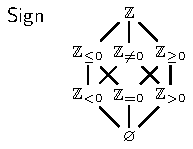
\includegraphics{sign-domain.pdf}
	\end{center}
	The meaning of each abstract elements of $\Sign$ is to represent concrete values that satisfy the respective property: for instance, $\gamma(\setZ_{< 0}) = \{ n \in \setZ \svert n < 0 \}$ and $\alpha( \{ 0; 1; 100 \}) = \setZ_{\ge 0}$.
	The bca of a concrete function $f: \pow(\setZ) \to \pow(\setZ)$ is defined as $f^{\Sign}\eqdef \alpha~f~\gamma: \Sign \to \Sign$.

	Consider the simple program fragment
	$$\regc \eqdef \code{x := x + 1; x := x - 1}\ .$$

	Its denotational semantics $\denot{\regc}$ is the identity function $\id_{\setZ}$, so its bca $$\denot{\regc}^{\Sign} \eqdef \alpha~\id_{\setZ}~\gamma = \id_{\Sign}$$
	is just the abstract identity. We say that $\denot{\regc}^{\Sign}$ is \emph{extensional} because it only depends on the function computed by $\regc$, i.e., its denotational semantics. However, an analyser does not know the semantics of $\regc$, so it has to analyse the program syntactically, breaking it down in elementary pieces and gluing the results together. So for instance, starting from the concrete point $P = \{ 1 \}$ the analysis first abstracts it to the property $\alpha(P) = \setZ_{> 0}$, then it computes
	\begin{align*}
		\denot{\regc}^{\sharp}_{\Sign} (\setZ_{> 0}) & = \denot{\code{x := x - 1}}^{\sharp}_{\Sign} \denot{\code{x := x + 1}}^{\sharp}_{\Sign} (\setZ_{> 0}) \\
		                                             & = \denot{\code{x := x - 1}}^{\sharp}_{\Sign} (\setZ_{> 0}) = \setZ_{\ge 0} .
	\end{align*}
	Analogous calculations for all properties in $\Sign$ yields the abstraction
	\[
	\denot{\regc}^{\sharp}_{\Sign}(a) = \begin{cases*}
		\varnothing   & if $a = \varnothing$                                                                                     \\
		\setZ_{\ge 0} & if $a \in \{ \colorbox{lightgray}{$\setZ_{= 0}$}, \colorbox{lightgray}{$\setZ_{> 0}$}, \setZ_{\ge 0} \}$ \\
		\setZ_{< 0}   & if $a = \setZ_{< 0}$                                                                                     \\
		\setZ         & if $a \in \{ \colorbox{lightgray}{$\setZ_{\le 0}$}, \colorbox{lightgray}{$\setZ_{\neq 0}$}, \setZ \}$
	\end{cases*}
	\]
	that, albeit sound, is less precise than $\id_{\Sign}$ (we highlight with a gray background all inputs on which $\denot{\regc}^{\sharp}_{\Sign}$ loses accuracy).

	The program $\regc$ is equivalent to the command $\code{skip}$, because $\denot{\code{skip}}=\id_{\setZ}$, and thus $\regc$ and $\code{skip}$ are assigned the same bca $\denot{\code{skip}}^{\Sign} = \denot{\code{skip}}^{\Sign} =  \id_{\Sign}$.
	However, $\denot{\code{skip}}^{\sharp}_{\Sign} = \id_{\Sign} \neq \denot{\regc}^{\sharp}_{\Sign}$, exposing the \emph{intensional} essence of the abstract interpreter: the abstraction depends on how the program is written and not only on its semantics.\footnote{While it falls outside the scope of this thesis, we refer the interested reader to, e.g.,~\cite{BGGGP19,BRZ22} for more about intensional and extensional abstract properties.}
\end{example}

The possibility of weakening point~(3) from being an intensional requirement based on $\denot{\regc}^{\sharp}_A$ to an extensional one based on bcas $\denot{\regc}^A$ has several nice consequences.
First, the local completeness of $\denot{\regc}^A$ is enough to guarantee that points~(1-2) hold.
Second, while the proof system itself provides an intensional analysis, because its rules are defined inductively on the program syntax, the information it produces is more precise, in the sense that the property associated with triples is extensional: no precision is lost because of the approximation introduced by the intensional abstract interpreter.
Third, it allows the proof system to derive more triples than the original one, because bcas can be locally complete also in cases where the abstract interpreter is not (but not vice versa).
Finally, since extensional properties are irrespective of how the program is written, this possibility provides the potential for deriving exactly the same triples for equivalent programs.

Lastly, the whole theory of completeness in abstract interpretation is based on the framework of Galois connection. Therefore, $\LCLA$ cannot be applied to known instances of abstract domains lacking an abstraction function $\alpha$, such as convex polyhedra abstractions~\cite{CH78} that are widely used in static analysis. However, abstract convexity of local completeness can help mitigate this limitation: even if a point doesn't have a best abstraction, if it can be bound between another point and its abstraction, we can in a sense ``prove'' local completeness on it thanks to abstract convexity.

\section{Extensional soundness}
As anticipated at the beginning of the Chapter, one of our goals is to weaken point (3) of the soundness Theorem~\ref{th:sota:lcl-soundness} from local completeness of the abstract interpreter $\denot{\regr}^{\sharp}_A$ to that of the bca $\denot{\regr}^A$. The key observation is that the proof of Corollary~\ref{th:sota:corollary-verification} only relies on points (1-2) of Theorem~\ref{th:sota:lcl-soundness}, so from a program analysis perspective point (3) can be seen as a technical requirement to prove the other two. However, we observe that local completeness of the bca is enough to this aim: we therefore present a slightly weaker\footnote{Logically speaking, we prove a stronger conclusion, so the theorem as an implication is weaker.} soundness result for $\LCLA$, with the bca $\denot{\regr}^A$ in place of the inductively defined abstract interpreter $\denot{\regr}^{\sharp}_A$.

\begin{theorem}[Extensional soundness]\label{th:lcla:soundness-ext}
	Let $A_{\alpha, \gamma} \in \Abs(C)$.
	If $\lcl{A}{P}{\regr}{Q}$ then:
	\begin{enumerate}
		\item $Q \le \denot{\regr} P$,
		\item $\alpha(\denot{\regr} P) = \alpha(Q)$,
		\item $\denot{r}^A \alpha(P) = \alpha(Q)$.
	\end{enumerate}
\end{theorem}
\begin{proof}
	First we remark that points (1) and (3) implies point (2):
	\begin{align*}
		\alpha(Q) & \le \alpha(\denot{\regr} P)     & [\text{(1) and monotonocity of }\alpha] \\
		          & \le \denot{\regr}^{A} \alpha(P) & [\text{soundness of }\denot{\regr}^{A}] \\
		          & = \alpha(Q)                     & [\text{(3)}]
	\end{align*}
	So all the lines are equal, in particular $\alpha(Q) = \alpha(\denot{\regr} P)$.
	The proof is then by induction on the derivation tree of $\lcl{A}{P}{\regr}{Q}$, but we only have to prove (1) and (3) because of the observation above.
	We only include one inductive case as an example; the full proof is in Appendix~\ref{ch:app:lcla}.

	\proofcase{\lclrule{seq}}
	\noindent (1) $Q \le \denot{\regr_2} R \le \denot{\regr_2} (\denot{\regr_1} P) = \denot{\regr1; \regr_2} P$, where the inequalities follow from inductive hypotheses and monotonicity of $\denot{\regr_2}$.

	\noindent (3) We recall that $\denot{\regr_1; \regr_2}^{A} \le \denot{\regr_2}^{A} \denot{\regr_1}^{A}$.
	\begin{align*}
		\alpha(Q) & \le \alpha(\denot{\regr_1; \regr_2} P)                & [\text{(1) and monotonicity of }\alpha] \\
		          & \le \denot{\regr_1; \regr_2}^{A} \alpha(P)            & [\text{soundness of }\denot{\regr}^{A}] \\
		          & \le \denot{\regr_2}^{A} \denot{\regr_1}^{A} \alpha(P) & [\text{recalled above}]                 \\
		          & = \denot{\regr_2}^{A} \alpha(R)                       & [\text{inductive hp}]                   \\
		          & = \alpha(Q)                                           & [\text{inductive hp}]
	\end{align*}
	So all the lines are equal, in particular $\denot{\regr_1; \regr_2}^{A} \alpha(P) = \alpha(Q)$.
\end{proof}

Theorem~\ref{th:sota:lcl-soundness} involves $\denot{\regr}^{\sharp}_A$, an \emph{intensional} property of the program $\regr$ that depends on how the program is written, while the new statement we propose here relies only on $\denot{\regr}^A$, an \emph{extensional} property of the computed function $\denot{\regr}$ and not of $\regr$ itself.
Accordingly, for the rest of this chapter we use the name \emph{intensional soundness} for the former and \emph{extensional soundness} for the latter.
Again, we say a triple is \emph{extensionally valid} if it satisfies point (1--3) of Theorem~\ref{th:lcla:soundness-ext} above, and intensionally valid for the former notion introduced in Section~\ref{sec:sota:lcl}. We shall write $\lclvalid{A}{P}{\regr}{Q}$ for both, but we will make sure to disambiguate the notation when not clear from the context.

\section{Locally complete refinement}
\begin{figure*}[t]
	\begin{framed}
		\[
		\infer[\lclrule{refine\mbox{-}ext}]
		{\lcl{A}{P}{\regr}{Q}}
		{\lcl{A'}{P}{\regr}{Q} & A' \preceq A & A \denot{\regr}^{A'} A(P) = A(Q)}
		\]
	\end{framed}
	\vspace{-1ex}
	\caption{Rule \lclrule{refine\mbox{-}ext} for $\LCLA$.}\label{fig:lcla:rule-refine}
\end{figure*}

Our aim is to enhance the original $\LCLA$ proof system to handle triples where the extensional abstraction $\denot{\regr}^{A}$ is proved to be locally complete w.r.t. the given input, that is $\denot{\regr}^{A} \alpha(P) = \alpha(\denot{\regr} P)$. To achieve this, we extend the proof system with a new inference rule, that is shown in Figure~\ref{fig:lcla:rule-refine}. It is named after ``refine'' because it allows to refine the abstract domain $A$ to some $A' \preceq A$ (see Section~\ref{sec:bg:absint}) and ``ext'' since it involves the extensional bca $\denot{\regr}^{A'}$ of $\denot{\regr}$ in $A'$ (to distinguish it from the rules we will introduce later).

Using \lclrule{refine\mbox{-}ext} it is possible to construct a derivation that proves local completeness of portions of the whole program in a more precise abstract domain $A'$ and then carries the result over to the global analysis in a coarser domain $A$. The only requirement for the application of the rule is that the domain $A'$ satisfies $A \denot{\regr}^{A'} A(P) = A(Q)$.

Formally, given the two abstract domains $A_{\alpha, \gamma}, A'_{\alpha', \gamma'} \in \Abs(C)$, this last premise of rule \lclrule{refine\mbox{-}ext} should be written as $\alpha \gamma' \denot{\regr}^{A'} \alpha' A(P) = \alpha(Q)$. However we prefer the more concise, albeit a little imprecise, notation in Figure~\ref{fig:lcla:rule-refine}. That notation is justified by the following intuitive argument: since $A' \preceq A$ we can consider, with a slight abuse of notation (seeing abstract domains as closures) $A \subseteq A' \subseteq C$, so that for any element $a \in A \subseteq C$ we have $\gamma(a) = \gamma'(a) = a$ and for any $c \in C$ we have $\alpha' A(c) = A(c)$. With these
\[
\alpha \gamma' \denot{\regr}^{A'} \alpha' A(P) = \alpha \denot{\regr}^{A'} A(P) = A \denot{\regr}^{A'} A(P) .
\]

With the addition of rule \lclrule{refine\mbox{-}ext}, intensional soundness (Theorem~\ref{th:sota:lcl-soundness}) does not hold anymore: since this rule allows to perform part of the analysis in a more concrete domain $A'$, we do not get any information on $\denot{\regr}^{\sharp}_A$. However, rule \lclrule{refine\mbox{-}ext} is sound w.r.t. the bca $\denot{\regr}^A$, and therefore it makes the proof system extensionally sound:

\begin{theorem}[Extensional soundness of \lclrule{refine\mbox{-}ext}]\label{th:lcla:soundness-rule-refine}
	The proof system in Figure~\ref{fig:sota:lcla-rules} with the addition of rule \lclrule{refine\mbox{-}ext} from Figure~\ref{fig:lcla:rule-refine}) is extensionally sound.
\end{theorem}
\begin{proof}[Proof sketch]
	We extend the proof of Theorem~\ref{th:lcla:soundness-ext} with a new inductive case. The full details are in Appendix~\ref{ch:app:lcla}.
\end{proof}

We remark that a rule like \lclrule{refine\mbox{-}ext}, that allows to carry on part of the proof in a different abstract domain, cannot be unconstrained. We present an example showing that an analogous inference rule only requiring the triple $\lcl{}{P}{\regr}{Q}$ to be provable in an abstract domain $A' \preceq A$ without any further constraint would be unsound.
\begin{example}
	Consider the concrete domain $C = \pow(\setZ)$ of integers, the point $P = \{ -5; -1 \}$, the abstract domain $\Sign$ of Example~\ref{ex:lcla:ext-vs-int} and the program
	\[
	\regr \eqdef \code{x := x + 10} .
	\]
	Then $C \preceq \Sign$ and we can prove $\lcl{C}{P}{\regr}{\{ 5; 9 \}}$ applying \lclrule{transfer} since all functions are locally complete in the concrete domain. However, if $f = \denot{\regr} = \edenot{\code{x := x + 10}}$, it is not the case that $\complete{\Sign}{P}{f}$: indeed
	\begin{align*}
		\Sign (f (\Sign(P))) & = \Sign (f(\setZ_{< 0})) = \Sign(\{ n \in \setZ \svert n < 10 \}) = \top
	\end{align*}
	while
	\begin{align*}
		\Sign(f(P)) & = \Sign(\{ 5, 9 \}) = \setZ_{> 0}.
	\end{align*}
	This means that a refinement rule without any additional condition is unsound because it would allow to prove triples which are not locally complete.
\end{example}

\subsection{Logical completeness}\label{sec:logical-completeness}
Among all the possible conditions that make a refinement rule valid, we believe ours to be very general since the \lclrule{refine\mbox{-}ext} allows us to derive logical completeness, i.e., the ability to prove \emph{any} triple satisfying the soundness properties guaranteed by the proof system. Note that this was not the case for the original $\LCLA$ proof system~\cite[§5.2]{BGGR21}.

%In Section~5.2 of \cite{BGGR21}, the authors discuss logical completeness of $\LCLA$. Here the adjective ``logical" is used to disambiguate the term with respect to Abstract interpretation completeness.
%: the former is about the class of triples that can be proved in the proof system, while the latter is the extensively discussed concept of not losing precision in an analysis.
However, to prove such a result, our extension need an additional rule to handle loops, just like the original $\LCLA$ and IL.
The necessary infinitary rule, called \lclrule{limit}, allows the proof system to handle Kleene star, and is the same as $\LCLA$:

\[\infer[(\mathsf{limit})]
{\lcl{A}{P_0}{\regr^\kstar}{\bigvee_{i \ge 0}P_i}}
{\forall n \ge 0 \svert \lcl{A}{P_n}{\regr}{P_{n+1}}}
\]
\begin{theorem}[Logical completeness of \lclrule{refine\mbox{-}ext}]\label{th:lcla:refinement-rule-completeness}
	Consider the proof system of Figure~\ref{fig:sota:lcla-rules} with the addition of rules \lclrule{refine\mbox{-}ext} and \lclrule{limit}. If $Q \le \denot{\regr} P$ and $\denot{\regr}^A \alpha(P) = \alpha(Q)$ then $\lcl{A}{P}{\regr}{Q}$.
\end{theorem}
\begin{proof}
	First, the hypotheses of the theorem implies $\complete{A}{P}{\denot{\regr}}$:
	\begin{align*}
		\denot{\regr}^A \alpha(P) & = \alpha(Q)                   & [\text{hp of the theorem}]                                             \\
		                          & \le \alpha(\denot{\regr} P)   & [\text{monotonicity of } \alpha \text{ and hp } Q \le \denot{\regr} P] \\
		                          & \le \denot{\regr}^A \alpha(P) & [\text{soundness of } \denot{\regr}^{A}]
	\end{align*}
	Hence $\alpha(\denot{\regr} P) = \denot{\regr}^A \alpha(P) = \alpha \denot{\regr} \gamma \alpha(P)$, that is local completeness, and $\alpha(Q) = \alpha(\denot{\regr} P)$.

	Now consider $\regr, P, Q$ satisfying the hypotheses. If $Q < \denot{\regr} P$, by \lclrule{relax} we get
	\[
	\infer[(\mathsf{relax})]
	{\lcl{A}{P}{\regr}{Q}}
	{P \le P \le A(P) & \lcl{A}{P}{\regr}{\denot{\regr} P} & Q \leq \denot{\regr} P \le A(Q)}
	\]
	But the first condition is trivial, and the third one is made of $Q \le \denot{r}P$ (the hypothesis) and $\denot{r} P \le A(Q)$, that follows because $\alpha(\denot{r} P) = \alpha(Q)$ (shown above) and in a Galois connection this implies $\denot{r} P \le \gamma \alpha(Q) = A(Q)$. Hence, without loss of generality, we can assume $Q = \denot{\regr} P$.

	Now we want to apply \lclrule{refine\mbox{-}ext} to move to the concrete domain $C$. Clearly $C \preceq A$. The last hypothesis of the rule can be readily verified recalling that $\denot{r}^{C} = \denot{r}$ and $\alpha' = \gamma' = \id_C$:
	\begin{align*}
		\alpha \denot{r}^{C} A(P) & = \alpha \denot{r} A(P)   \\
		                          & = \denot{r}^{A} \alpha(P) \\
		                          & = \alpha(\denot{\regr} P)
	\end{align*}
	To say that triple $\lcl{C}{P}{\regr}{\denot{\regr} P}$ is provable we resort to Theorem~5.11 of \cite{BGGR21}. The hypothesis of that theorem are satisfied: all expressions are globally complete in the concrete domain $C$, $\denot{r} P \le \denot{r} P$ and $\denot{r}^{\sharp}_C \id_C(P) = \denot{\regr} P = \id_C(\denot{r} P)$, where we used $\alpha' = \id_C$ and $\denot{r}^{\sharp}_C = \denot{r}$.

	Thus, by applying \lclrule{refine\mbox{-}ext}, we can prove the triple $\lcl{A}{P}{\regr}{\denot{\regr} P}$:
	\[
	\infer[(\mathsf{refine\mbox{-}ext})]
	{\lcl{A}{P}{\regr}{\denot{\regr} P}}
	{\lcl{C}{P}{\regr}{\denot{\regr} P} & C \preceq A & A \denot{\regr}^{C} A(P) = A(\denot{\regr} P)}
	\]
\end{proof}

The previous theorem proves the logical completeness of our proof system with respect to extensional validity: indeed, if $Q \le \denot{\regr} P$ and $\denot{\regr}^A \alpha(P) = \alpha(Q)$ we also have:
\begin{align*}
	\alpha(Q) \le \alpha(\denot{\regr} P) \le \denot{\regr}^{A} \alpha(P) = \alpha(Q) ,
\end{align*}
hence all three conditions of Theorem~\ref{th:lcla:soundness-ext} are satisfied.

An interesting consequence of this result is the existence of a refinement $A'$ in which it is possible to carry out the proof. In principle, such a refinement could be the concrete domain $C$ (as shown in the proof), that is not computable. However, it is worth nothing that for a sequential fragment (a portion of code without loops) the concrete domain can be actually used (for instance via first-order logic). This opens up the possibility, for instance, to infer a loop invariant on the body using $C$, and then prove it using an abstract domain.
In Section~\ref{sec:lcla:choose-refinement} we discuss this issue further.

\subsection{Derived refinement rules}\label{sec:lcla:derived-rules}

The hypothesis $A \denot{\regr}^{A'} A(P) = A(Q)$ is added to rule \lclrule{refine\mbox{-}ext} in order to guarantee soundness: in general, the ability to prove a triple such as $\lcl{}{P}{\regr}{Q}$ in a refined domain $A'$ only gives information on $A \denot{\regr}^{A'} A'(P)$ but not on $A \denot{\regr}^{A'} A(P)$. In fact, the example below shows that $A \denot{\regr}^{A'} A'(P) $ and $A \denot{\regr}^{A'} A(P)$ can be different.

\begin{example}\label{ex:lcla:bound-A'-not-A}
	Consider the concrete domain $\pow(\setZ)$, the abstract domain of signs $\Sign_{\alpha, \gamma} \in \Abs(\pow(\setZ))$ (introduced in Example~\ref{ex:lcla:ext-vs-int}) and its refinement $\Sign_{1}$ below:

	\begin{center}
		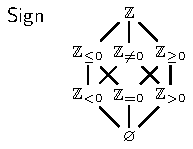
\includegraphics{sign-domain.pdf}
		\qquad\qquad
		% \begin{tikzpicture}[scale=0.7,shorten >=-2pt, shorten <=-2pt]
		% 	\draw (-1,-1) node[name=1] {\footnotesize$\varnothing$};
		% 	\draw (-2,0.2) node[name=2] {\footnotesize$\setZ_{<0}$};
		% 	\draw (-1,0.2) node[name=3] {\footnotesize$\setZ_{=0}$};
		% 	\draw (0,-0.3) node[name=9] {\footnotesize$\setZ_{=1}$};
		% 	\draw (0,0.6) node[name=4] {\footnotesize$\setZ_{>0}$};
		% 	\draw (-2,1.8) node[name=5] {\footnotesize$\setZ_{\leq 0}$};
		% 	\draw (-1,1.8) node[name=8] {\footnotesize$\setZ_{\neq 0}$};
		% 	\draw (-0,1.8) node[name=6] {\footnotesize$\setZ_{\geq 0}$};
		% 	\draw (-1,3) node[name=7] {\footnotesize$\setZ$};
		% 	\draw (-3,2.9) node[name=n] {{\normalsize $\Sign_1$}};
		%
		%
		% 	\draw[semithick] (1) -- (2);
		% 	\draw[semithick] (1) -- (3);
		% 	\draw[semithick] (2) -- (5);
		% 	\draw[semithick] (2) -- (8);
		% 	\draw[semithick] (3) -- (5);
		% 	\draw[semithick] (3) -- (6);
		% 	\draw[semithick] (4) -- (6);
		% 	\draw[semithick] (4) -- (8);
		% 	\draw[semithick] (5) -- (7);
		% 	\draw[semithick] (6) -- (7);
		% 	\draw[semithick] (8) -- (7);
		% 	\draw[semithick] (1) -- (9);
		% 	\draw[semithick] (9) -- (4);
		% \end{tikzpicture}
		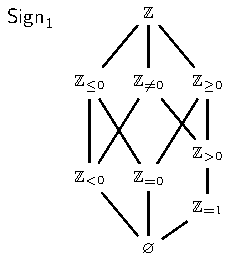
\includegraphics{sign1-domain.pdf}
	\end{center}

	For the command $\regr \eqdef \code{x := x - 1}$ and the concrete point $P = \{ 1 \}$ we have
	\[
	\Sign \denot{\regr}^{\Sign_{1}} \Sign_1(P) = \Sign \denot{\regr}^{\Sign_{1}} (\setZ_{= 1}) = \setZ_{= 0}
	\]
	but
	\[
	\Sign \denot{\regr}^{\Sign_1} \Sign(P) = \Sign \denot{\regr}^{\Sign_1} (\setZ_{> 0}) = \setZ_{\ge 0} .
	\]
\end{example}

Despite being necessary, the hypothesis of rule \lclrule{refine\mbox{-}ext} cannot be checked algorithmically because, in general, the bca $\denot{\regr}^{A'}$ of a composite command $\regr$ is not computable. To mitigate this issue, we present two derived rules whose premises imply the premises of Rule \lclrule{refine\mbox{-}ext}, hence ensuring extensional soundness by means of Theorem~\ref{th:lcla:soundness-rule-refine}.

\begin{figure*}[t]
	\begin{framed}
		\[
		\infer[\lclrule{refine\mbox{-}int}]
		{\lcl{A}{P}{\regr}{Q}}
		{\lcl{A'}{P}{\regr}{Q} \quad A' \preceq A \quad A \denot{\regr}^{\sharp}_{A'} A(P) = A(Q) }
		\]
	\end{framed}
	\vspace{-1ex}
	\caption{Rule \lclrule{refine\mbox{-}int} for $\LCLA$.}\label{fig:lcla:rule-refine-int}
\end{figure*}

The first rule we present replaces the requirement on the extensional bca $\denot{\regr}^{A'}$ with requirements on the intensional compositional abstraction $\denot{\regr}^{\sharp}_{A'}$ computed in $A'$ (see Figure~\ref{fig:lcla:rule-refine-int}). For this reason, we call this rule \lclrule{refine\mbox{-}int}.

\begin{prop}\label{th:lcla:refine-int-sound}
	The rule \lclrule{refine\mbox{-}int} in Figure~\ref{fig:lcla:rule-refine-int} is extensionally sound.
\end{prop}
\begin{proof}[Proof sketch]
	We show that the hypotheses of \lclrule{refine\mbox{-}int} implies those of \lclrule{refine\mbox{-}ext}. Since the first two hypotheses $\lcl{A'}{P}{\regr}{Q}$ and $A' \preceq A$ are shared among the two rules, we only have to show that $\alpha \gamma' \denot{\regr}^{A'} \alpha' A(P) = \alpha(Q)$. The details of this are in Appendix~\ref{ch:app:lcla}.

	Because the hypotheses of \lclrule{refine\mbox{-}int} implies those of \lclrule{refine\mbox{-}ext}, whenever we can apply the former we can also apply the latter, so that Theorem~\ref{th:lcla:soundness-rule-refine} ensures extensional soundness.
\end{proof}

It is worth noting that the condition on the compositional abstraction $\denot{\regr}^{\sharp}_{A'}$ can easily be checked by the analyser, possibly alongside the analysis of $\regr$ with LCL or using a stand-alone abstract interpreter.
Moreover, this rule is as powerful as the original \lclrule{refine\mbox{-}ext} because it enjoys a logical completeness result akin to Theorem~\ref{th:lcla:refinement-rule-completeness}.
\begin{theorem}[Logical completeness of \lclrule{refine\mbox{-}int}]\label{th:lcla:refine-int-completeness}
	Consider the proof system of Figure~\ref{fig:sota:lcla-rules} with the addition of rules \lclrule{refine\mbox{-}int} and \lclrule{limit}. If $Q \le \denot{\regr} P$ and $\denot{\regr}^A \alpha(P) = \alpha(Q)$ then $\lcl{A}{P}{\regr}{Q}$.
\end{theorem}
\begin{proof}
	The proof is the same as Theorem~\ref{th:lcla:refinement-rule-completeness}, the only difference being that to apply \lclrule{refine\mbox{-}int} we need to show $A \denot{\regr}^{\sharp}_{C} A(P) = A(\denot{\regr} P)$ instead of $A \denot{\regr}^{C} A(P) = A(\denot{\regr} P)$. However, since in the concrete domain $\denot{\regr}^{\sharp}_{C} = \denot{\regr}^{C} = \denot{\regr}$ the proof still holds.
\end{proof}

Just like logical completeness of \lclrule{refine\mbox{-}ext}, this result implies the existence of a refinement $A'$ (possibly the concrete domain) in which it is possible to carry out the proof.

\begin{figure*}[t]
	\begin{framed}
		\[
		\infer[\lclrule{refine\mbox{-}pre}]
		{\lcl{A}{P}{\regr}{Q}}
		{\lcl{A'}{P}{\regr}{Q} \quad A' \preceq A \quad A'(P) = A(P) }
		\]
	\end{framed}
	\vspace{-1ex}
	\caption{Rule \lclrule{refine\mbox{-}pre} for $\LCLA$.}\label{fig:lcla:rule-refine-pre}
\end{figure*}

The second derived rule we propose (see Figure~\ref{fig:lcla:rule-refine-pre}) is simpler than \lclrule{refine\mbox{-}ext}: it just requires the abstractions $A(P)$ and $A'(P)$ to coincide, with no reference to the regular command $\regr$ nor to the postcondition $Q$. Since the premise is only on the precondition $P$, we call this rule \lclrule{refine\mbox{-}pre}.

\begin{prop}\label{th:lcla:refine-pre-sound}
	The rule \lclrule{refine\mbox{-}pre} in Figure~\ref{fig:lcla:rule-refine-pre} is extensionally sound.
\end{prop}
\begin{proof}[Proof sketch]
	The proof follows the same line as Proposition~\ref{th:lcla:refine-int-sound}. The details are in Appendix~\ref{ch:app:lcla}.
\end{proof}

Rule \lclrule{refine\mbox{-}pre} only requires a simple check at the application site instead of an expensive analysis of the program $\regr$, so it can be preferable in practice.

We present an example to highlight the advantages of this rule (as well as \lclrule{refine\mbox{-}int}), which allows us to use different domains in the proof derivation of different parts of the program.

\begin{example}[The use of \lclrule{refine\mbox{-}pre}]\label{ex:lcla:refine-pre-usefulness}
	Consider the two program fragments
	\begin{align*}
		\regr_1 & \eqdef \code{(y != 0)?; y := abs(y)}                                       \\
		\regr_2 & \eqdef \code{x := y; while (x > 1) \{ y := y - 1; x := x - 1 \}}           \\
		        & = \code{x := y; ((x > 1)?; y := y - 1; x := x - 1)$^{\kstar}$; (x <= 1)? }
	\end{align*}
	and the program $\regr \eqdef \regr_1; \regr_2$. Here \code{abs} is a function to compute the absolute value, and we assume, for the sake of simplicity, that the analyser knows its best abstraction. Consider the concrete domain $\pow(\setZ^2)$ where a pair $(n, m)$ denote a state $\code{x} = n$, $\code{y} = m$, and the initial state $P = (\code{y} \in [-100; 100])$, a logical description of the concrete points $\{ (n, m) \svert m \in [-100; 100] \} \in \pow(\setZ^2)$.
	The bca $\denot{\regr}^{\Int}$ in the abstract domain of intervals is locally complete on $P$ (since $P$ is expressible in $\Int$), but the compositional abstraction $\denot{\regr}^{\sharp}_{\Int}$ is not:
	\begin{align*}
		\denot{\regr}^{\Int} \alpha(P) & = \Int (\denot{\regr_2} \denot{\regr_1} (\{ (n, m) \svert m \in [-100; 100] \})) \\
		                               & = \Int (\denot{\regr_2} (\{ (n, m) \svert m \in [1; 100] \}))                    \\
		                               & = \Int (\{ (1, 1) \})                                                            \\
		                               & = ([1; 1] \times [1; 1]) ,
	\end{align*}
	while
	\begin{align*}
		\denot{\regr}^{\sharp}_{\Int} \alpha(P) & = \denot{\regr_2}^{\sharp}_{\Int} \denot{\regr_1}^{\sharp}_{\Int} ([-\infty; +\infty] \times [-100; 100])   \\
		                                        & = \denot{\regr_2}^{\sharp}_{\Int} \denot{\code{y := abs(y)}}^{\Int} ([-\infty; +\infty] \times [-100; 100]) \\
		                                        & = \denot{\regr_2}^{\sharp}_{\Int} ([-\infty; +\infty] \times [0; 100])                                      \\
		                                        & = ([1; 1] \times [0; 100]) \neq ([1; 1] \times [1; 1]) .
	\end{align*}
	The issues are twofold.
	First, the analysis of $\regr_1$ in $\Int$ is incomplete, so we need a more concrete domain. For instance, we can select $\Int_{\neq 0}$, the Moore closure of $\Int$ with the addition of the element $\setZ_{\neq 0}$ representing the property of being nonzero. Intuitively, $\Int_{\neq 0}$ contains all intervals, possibly having a ``hole" in $0$. Formally
	\[
	\Int_{\neq 0} = \Int \cup \{ I_{\neq 0} \svert I \in \Int \}
	\]
	with $\gamma'(I_{\neq 0 }) = \gamma(I) \setminus \{ 0 \}$.

	While there is no need for a relational domain to analyse $\regr_1$ since  variable \code{x} is never mentioned in it,
	the analysis of $\regr_2$ requires a relational domain to track the information that the value of variable \code{x} is equal to the value of variable \code{y}.
	This suggests to use the octagons domain $\Oct$~\cite{Mine06} to analyse $\regr_2$. It is worth noting that the abstract domain $\Oct$ would not be able to perform a locally complete analysis of $\regr_1$ for the same reasons that the domain $\Int$ could not.

	However, rule \lclrule{refine\mbox{-}pre} allows us to combine these different proof derivations. Since the program state between $\regr_1$ and $\regr_2$ can be precisely represented in $\Int$, we use this domain as a baseline and refine it to $\Int_{\neq 0}$ and to $\Oct$ for the two parts, respectively.

	%	\begin{figure*}[t]
	%		\[
	%		\text{\small
	%			\infer[(\mathsf{seq})]
	%			{\lcl{\Int_{\neq 0}}{P}{\regr_1}{R}
	%					\qquad \Int_{\neq 0} \preceq \Int \qquad \Int(P) = \Int_{\neq 0}(P)
	%			}
	%			{
	%				\infer[(\mathsf{transfer})]
	%				{\lcl{\Int_{\neq 0}}{P}{\code{y != 0?}}{R_1}}{ \complete{\Int_{\neq 0}}{P}{\denot{\code{y != 0?}}} }
	%				&
	%				\infer[(\mathsf{relax})]
	%				{\lcl{\Int_{\neq 0}}{R_1}{\code{y := abs(y)}}{R}}
	%				{\infer[(\mathsf{transfer})]
	%					{\lcl{\Int_{\neq 0}}{R_1}{\code{y := abs(y)}}{\code{y} \in [1; 100]}}{ \complete{\Int_{\neq 0}}{R_1}{\denot{\code{y := abs(y)}}} }
	%				}
	%			}
	%		}
	%		\]
	%		\caption{Derivation of $\lcl{\Int_{\neq 0}}{P}{\regr_1}{R}$ for Example~\ref{ex:refine-pre-usefulness}.}\label{fig:ex-refine-pre-derivation-1}
	%	\end{figure*}

	Let $R = (\code{y} \in \{ 1; 2; 100 \})$ that is an under\hyp{}approximation of the concrete state in between $\regr_1$ and $\regr_2$ with the same abstraction in $\Int$, so the triple $\lcl{\Int}{P}{\regr_1}{R}$ is valid. Note that the concrete point $2$ was added to $R$ in order to have local completeness for \code{(x > 1)?} in $\regr_2$. However, this triple cannot be proved in $\Int$ because $\denot{\regr_1}^{\sharp}_{\Int}$ is not locally complete on $P$, so we resort to \lclrule{refine\mbox{-}pre} to change the domain to $\Int_{\neq 0}$.
	In the derivation below, we let $R_1 = (\code{y} \in [-100; 100] \land \code{y} \neq 0)$ and we omit for simplicity the additional hypothesis of \lclrule{relax}:
	\[
	\infer[(\mathsf{seq})]
	{\lcl{\Int_{\neq 0}}{P}{\regr_1}{R}
		%					\qquad \Int_{\neq 0} \preceq \Int \qquad \Int(P) = \Int_{\neq 0}(P)
	}
	{
		\infer[(\mathsf{transfer})]
		{\lcl{\Int_{\neq 0}}{P}{\code{y != 0?}}{R_1}}{ \complete{\Int_{\neq 0}}{P}{\denot{\code{y != 0?}}} }
		&
		\infer[(\mathsf{relax})]
		{\lcl{\Int_{\neq 0}}{R_1}{\code{y := abs(y)}}{R}}
		{\infer[(\mathsf{transfer})]
			{\lcl{\Int_{\neq 0}}{R_1}{\code{y := abs(y)}}{\code{y} \in [1; 100]}}{ \complete{\Int_{\neq 0}}{R_1}{\denot{\code{y := abs(y)}}} }
		}
	}
	\]

	Again $\denot{\regr_2}$ is locally complete on $R$ in $\Int$, but the compositional analysis $\denot{\regr_2}^{\sharp}_{\Int}$ is not. Hence to perform the derivation we resort to \lclrule{refine\mbox{-}pre} to introduce relational information in the abstract domain, using $\Oct$ instead of $\Int$. Let $Q = (\code{x} = 1 \land \code{y} = 1)$, that is the concrete output of the program, so that we can prove $\lcl{\Int}{R}{\regr_2}{Q}$.
	The derivation of this triple is in Appendix~\ref{ch:app:lcla}, Figure~\ref{fig:app:ex-refine-pre-derivation-2}. However, the proof is just a straightforward application of rules \lclrule{seq}, \lclrule{iterate} and \lclrule{transfer}.

	With those two derivation, we can prove the triple $\lcl{\Int}{P}{\regr}{Q}$ using \lclrule{refine\mbox{-}pre}:
	\[
	\infer[(\mathsf{seq})]
	{\lcl{\Int}{P}{\regr}{Q}}
	{
		\infer[(\mathsf{refine\mbox{-}pre})]
		{\lcl{\Int}{P}{\regr_1}{R}}
		{\lcl{\Int_{\neq 0}}{P}{\regr_1}{R}}
		&
		\infer[(\mathsf{refine\mbox{-}pre})]
		{\lcl{\Int}{R}{\regr_2}{Q}}
		{\lcl{\Oct}{R}{\regr_2}{Q}}
	}
	\]
	For space constraints, we write here the additional hypotheses of the rules. For the first application, $\Int_{\neq 0} \preceq \Int$ and $\Int_{\neq 0}(P) = P = \Int(P)$. For the second, $\Oct \preceq \Int$ and $\Int(R) = (\code{y} \in [1; 100]) = \Oct(R)$.

	It is worth noting that, in this example, all applications of \lclrule{refine\mbox{-}pre} can be replaced by \lclrule{refine\mbox{-}int}. This means that also the latter is able to exploit $\Int_{\neq 0}$ and $\Oct$ to prove the triple in the very same way, but its application requires more expensive abstract analyses than the simple checks of \lclrule{refine\mbox{-}pre}.
\end{example}

While \lclrule{refine\mbox{-}pre} is simpler than \lclrule{refine\mbox{-}ext} and \lclrule{refine\mbox{-}int}, it is also weaker in both a theoretical and practical sense. On the one hand, $\LCLA$ extended with this rule does not admit a logical completeness result; on the other hand, there are situations in which, even though \lclrule{refine\mbox{-}pre} allows a derivation, \lclrule{refine\mbox{-}int} is more effective. We show these two points by examples.
For the first, we propose a valid triple that $\LCLA$ extended with \lclrule{refine\mbox{-}pre} cannot prove.

\begin{example}[Logical incompleteness of \lclrule{refine\mbox{-}pre}]\label{ex:lcla:refine-pre-incomplete}
	Consider the program fragments\footnote{Note that $\regr_w$ is equivalent to the regular command $\code{false?}$.}
	\begin{align*}
		\regr_1 & \eqdef \code{x := x + 2}              \\
		\regr_w & \eqdef \code{while (true) \{ skip \}} \\
		\regr   & \eqdef \regr_1 \code{; }\regr_w
	\end{align*}
	the concrete domain $\pow(\setZ)$, the abstract domains $\Int_{\neq 0}$ (see Example~\ref{ex:lcla:refine-pre-usefulness}) and the initial state $P = \{ -4, 0 \}$.
	Then $\lclvalid{\Int_{\neq 0}}{P}{\regr}{\emptyset}$ but this triple cannot be proved in $\LCLA$ extended with \lclrule{refine\mbox{-}pre}.

	To show that the triple is (intensionally) valid, we observe that
	\[
	\denot{\regr}^{\sharp}_{\Int_{\neq 0}} \alpha(P) = \denot{\regr_w}^{\sharp}_{\Int_{\neq 0}} \denot{\regr_1}^{\sharp}_{\Int_{\neq 0}} \alpha(P) = \bot
	\]
	because $\regr_w$ always diverges, so $\denot{\regr_w}^{\sharp}_{\Int_{\neq 0}}$ too is the function that always diverge (in the abstract). Therefore,
	\[
	\denot{\regr}^{\sharp}_{\Int_{\neq 0}} \alpha(P) = \alpha(\denot{\regr} P) = \alpha(\emptyset) = \bot .
	\]
	To show that the triple is not provable in $\LCLA$ extended with \lclrule{refine\mbox{-}pre}, we rely on two observations.

	The first is that all strict subset $P' \subset P$ are such that $\Int_{\neq 0}(P') \subset P$, and the same property holds for all refinements $A' \preceq \Int_{\neq 0}$. To see this, take $P' \subset P$: there are only three such $P'$, and for all of them $\Int_{\neq 0}(P') = P' \subset P$. Moreover, $A' \preceq \Int_{\neq 0}$ means that $A'(P') \subseteq \Int_{\neq 0}(P')$, so
	\[
	A'(P') \subseteq \Int_{\neq 0}(P') = P' \subset P .
	\]
	This property is important because it means that we cannot apply \lclrule{relax} to change $P$: to do it, we would need a $P' \subset P$ such that $P \subseteq A'(P')$.

	The second is that $\denot{\regr_1}$ is not locally complete on $P$ in $\Int_{\neq 0}$ or any of its refinements $A' \preceq \Int_{\neq 0}$ such that $A'(P) = \Int_{\neq 0}(P)$:
	\begin{align*}
		A'(\denot{\regr_1} P) & \subseteq \Int_{\neq 0}(\denot{\regr_1} P)      \\
		                      & = \{ -2, -1, 1, 2 \}                            \\
		                      & \subset \{ -2, -1, 0, 1, 2 \}                   \\
		                      & \subseteq A'(\{ -2, -1, 0, 1, 2 \})             \\
		                      & = A'(\denot{\regr_1} (\{ -4, -3, -2, -1, 0 \})) \\
		                      & = A'(\denot{\regr_1} (\Int_{\neq 0}(P)))        \\
		                      & = A'(\denot{\regr_1} A'(P))
	\end{align*}

	Now suppose to have a derivation of $\lcl{\Int_{\neq 0}}{P}{\regr}{\emptyset}$. This proof must use \lclrule{seq} to handle the sequential composition $\regr_1 \code{; }\regr_w$, so it needs a triple for $\regr_1$. By the first observation above, any use of \lclrule{relax} cannot change the precondition of this triple, even if we resort first to \lclrule{refine\mbox{-}pre} to refine the domain. Thus we must have a triple $\lcl{A'}{P}{\regr_1}{R}$ for some $R$ and $A' \preceq \Int_{\neq 0}$ satisfying $A'(P) = \Int_{\neq 0}(P)$. However, by soundness, any such triple would imply local completeness of $\denot{\regr_1}$ on $P$ in $A'$, which is a contradiction by the second observation above.
\end{example}

Another example of a sound triple which is not provable using \lclrule{refine\mbox{-}pre}, which does not rely on divergence, is in Appendix~\ref{ch:app:lcla}, Example~\ref{ex:app:refine-pre-incomplete-2-appendix}.
A corollary of these examples (and more in general of logical incompleteness) is that there may not exist a refinement $A'$ to carry out the proof using \lclrule{refine\mbox{-}pre}.
Another consequence of this incompleteness result is the fact that, even when a command is locally complete in an abstract domain $A$, we may need to reason about properties that are not expressible in $A$ in order to prove it, as \lclrule{refine\mbox{-}pre} may not be sufficient.

We now present an example to illustrate that there are situations in which \lclrule{refine\mbox{-}int} is more practical than \lclrule{refine\mbox{-}pre}, even though they are both able to prove the same triple.
\begin{example}
	Consider the two program fragments
	\begin{align*}
		\regr_1 & \eqdef \code{(y != 0)?; x := y; y := abs(y)}                     \\
		\regr_2 & \eqdef \code{x := y; while (x > 1) \{ y := y - 1; x := x - 1 \}}
	\end{align*}
	and the program $\regr \eqdef \regr_1; \regr_2$. Consider also the initial state $P = \code{y} \in [-100; 100]$.

	This example is a variation of Example~\ref{ex:lcla:refine-pre-usefulness}: the difference is the introduction of the relational dependency \code{x := y} in $\regr_1$, that is partially stored in the postcondition $R$ of $\regr_1$. Because of this, $\Oct(R)$ and $\Int(R)$ are different, so we cannot apply \lclrule{refine\mbox{-}pre} to prove $\lcl{}{R}{\regr_2}{Q}$ for some $Q$.

	%	We keep $\regr$ deliberately simple, but an actual program could do something between $\regr_1$ and $\regr_2$ with the value in \code{x}.

	Following Example~\ref{ex:lcla:refine-pre-usefulness}, the domain $\Int_{\neq 0}$ is able to infer on $\regr_1$ a subset $R$ of the strongest postcondition $\code{y} \in [1; 100] \land \code{y} = \text{abs}(\code{x})$ with the same abstraction $\Int_{\neq 0}(R) = [-100; 100]_{\neq 0} \times [1; 100]$. However, for any such $R$ we cannot use \lclrule{refine\mbox{-}pre} to prove the triple $\lcl{\Int}{R}{\regr_2}{\code{x} = 1 \land \code{y} = 1}$ via $\Oct$ because $\Int(R) = \code{x} \in [-100; 100] \land \code{y} \in [1; 100]$ while $\Oct(R) = 1 \le \code{y} \le 100 \land -\code{y} \le \code{x} \le \code{y}$. More in general, any subset of the strongest postcondition contains the relational information $\code{y} = \text{abs}(\code{x})$, so relational domains like octagons and polyhedra \cite{CH78} do not have the same abstraction as the non-relational $\Int$, preventing the use of \lclrule{refine\mbox{-}pre}. However, we can apply \lclrule{refine\mbox{-}int}: considering $R = (\code{y} \in \{1; 2; 100\} \land \code{y} = \text{abs}(\code{x}) )$, $Q = (\code{x} = 1 \land \code{y} = 1)$ and $\regr_w \eqdef \code{while (x > 1) \{ y := y - 1; x := x - 1 \}}$, we have
	\begin{align*}
		\Int \denot{\regr_2}^{\sharp}_{\Oct} \Int(R) & = \Int \denot{\regr_2}^{\sharp}_{\Oct} (\code{x} \in [-100; 100] \land \code{y} \in [1; 100])                                       \\
		                                             & = \Int \denot{\regr_w}^{\sharp}_{\Oct} \denot{\code{x := y}}^{\sharp}_{\Oct} (\code{x} \in [-100; 100] \land \code{y} \in [1; 100]) \\
		                                             & = \Int \denot{\regr_w}^{\sharp}_{\Oct} (1 \le \code{y} \le 100, \code{y} = \code{x})                                                \\
		                                             & = \Int(\code{x} = 1 \land \code{y} = 1)                                                                                             \\
		                                             & = \Int(Q) .
	\end{align*}

	In this example, rule \lclrule{refine\mbox{-}pre} can be applied to prove the triple, but it requires to have relational information from the assignment \code{x := y} in $\regr_1$, hence forcing the use of a relational domain (e.g. the reduced product~\cite{CC79} of $\Oct$ and $\Int_{\neq 0}$) for the whole $\regr$, making the analysis more expensive.
\end{example}

\subsection{Choosing the refinement}\label{sec:lcla:choose-refinement}
Thanks to the three new rules \lclrule{refine\mbox{-}ext}, \lclrule{refine\mbox{-}int} and \lclrule{refine\mbox{-}pre} we can now combine different domains in the same derivation.
However, in order to obtain an algorithm that automatises the search of a provable $\LCLA$ triple we are left with the problem of the selection of the right refinement to use each time. A crucial point to the applicability of refine rules is a strategy to find the most convenient refined abstract domain. While we have not addressed this problem yet, we believe there are some interesting starting points in the literature.

In previous sections, we settled the question from a theoretical point of view. Logical completeness results for \lclrule{refine\mbox{-}ext} (Theorem~\ref{th:lcla:refinement-rule-completeness}) and \lclrule{refine\mbox{-}int} (Theorem~\ref{th:lcla:refine-int-completeness}) implies the existence of a domain in which it is possible to complete the proof (if this were not the case, then the proof could not be completed in any domain, against logical completeness). However, the proofs of those theorems exhibit the concrete domain $C$ as an example, which is unfeasible in general. Dually, as \lclrule{refine\mbox{-}pre} is logically incomplete (Example~\ref{ex:lcla:refine-pre-incomplete}), there are triples that cannot be proved in any domain with it.

As more practical alternatives, we envisage some possibilities.
First, we are studying relationships with counterexample\hyp{}guided abstraction refinement (CEGAR) \cite{CGJLV00}, which is a technique that exploits refinement in the context of abstract model checking. However, CEGAR and our approach seem complementary. On the one hand, our refinement rules allow a dynamic change of domain, during the analysis and only for a part of it, while CEGAR performs a static refinement and then a new analysis of the whole transition system in the new, more precise domain. On the other hand, our rules lack an instantiation technique, while for CEGAR there are effective algorithms available to pick a suitable refinement.

Second, local completeness shell \cite{BGGR22} were proposed as an analogous of (global) completeness shell \cite{GRS00}. In the article, the authors proposed to use local completeness shells to perform abstract interpretation repair, a technique to refine the abstract domain depending on the program to analyse, just like CEGAR does for abstract model checking. Abstract interpretation repair works well with $\LCLA$, and could be a way to decide the best refinement for one of our rules in presence of a failed local completeness proof obligation. The advantage of combining repair with our new rules is given by the possibility of discarding the refined domain just after its use in a subderivation instead of using it to carry out the whole derivation. Investigations in this direction is ongoing.

Another related approach, which shares some common ground with CEGAR, is Lazy (Predicate) Abstraction \cite{HJMS02,McMillan06}. Both ours and this approach exploits different abstract domains for different parts of the proof, refining it as needed. The key difference is that Lazy Abstraction unwinds the control flow graph (CFG) of the program (with techniques to handle loops) while we work inductively on the syntax. This means that, when Lazy Abstraction refines a domain, it must use it from that point onward (unless it finds a loop invariant). On the other hand, our method can change abstract domain even for different parts of sequential code. However, the technique used in Lazy Abstraction (basically to trace a counterexample back with a theorem prover until it is either found to be spurious or proved to be true) could be applicable to $\LCLA$: a failed local completeness proof obligation in \lclrule{transfer} can be traced back with a theorem prover and the failed proof can be used to understand how to refine the abstract domain.

\section{Locally complete simplification}
\begin{figure*}[t]
	\begin{framed}
		\[
		\infer[\lclrule{simplify}]
		{\lcl{A}{P}{\regr}{Q}}
		{\lcl{A'}{P}{\regr}{Q} & A' \succeq A & A'(Q) = A(Q)}
		\]
	\end{framed}
	\vspace{-1ex}
	\caption{Rule \lclrule{simplify} for $\LCLA$.}\label{fig:lcla:rule-simplify}
\end{figure*}

We now turn our attention to \emph{simplification} of the abstract domain in the $\LCLA$ proof system. It is known that (global) completeness can be achieved both by refining and by simplifying the abstract domain (these construction are called completeness shell and core, respectively~\cite{GRS00}). Therefore, we do the same for local completeness.
We propose the rule \lclrule{simplify}, in Figure~\ref{fig:lcla:rule-simplify}. This is a dual of \lclrule{refine\mbox{-}pre}: while the latter requires $A'$ to be a refinement of $A$ with the same abstraction on the precondition $P$, the former requires $A'$ to be a simplification of $A$ with the same abstraction on the postcondition $Q$. We remark that this rule is independent of the refinement ones: it can be added to $\LCLA$ both with and without any of the refinement rules.

The proposed rule \lclrule{simplify} is sound, but differently than the refinement rules, it is so \emph{intensionally}:

\begin{theorem}[Intensional soundness of rule simplify]\label{th:lcla:soundness-rule-simpl}
	The proof system in Figure~\ref{fig:sota:lcla-rules} with the addition of rule \lclrule{simplify} from Figure~\ref{fig:lcla:rule-simplify} is intensionally sound.
\end{theorem}
\begin{proof}[Proof sketch]
	Since the proof of Theorem~\ref{th:sota:lcl-soundness} in~\cite{BGGR21} is by rule induction, we extend its proof with a new inductive case. The full details are in Appendix~\ref{ch:app:lcla}.
\end{proof}

This result is somewhat surprising: for completeness, refinement and simplification have the same power; instead, for local completeness, the former appears to be stronger than the former.

Even though rule \lclrule{simplify} does not allow the proof system to prove triples which are not intensionally sound, it still allows to prove more triples, as shown in the following example.

\begin{example}\label{ex:lcla:simplify-stronger}
	This example builds on the previous Example~\ref{ex:lcla:refine-pre-incomplete}.
	Consider the same program fragments $\regr_1$, $\regr_w$ and $\regr$, concrete domain $\pow(\setZ)$, abstract domain $\Int_{\neq 0}$, initial state $P = \{ -5, 0 \}$ and final state $\emptyset$.
	We already showed that the triple $\lcl{\Int_{\neq 0}}{P}{\regr}{\emptyset}$ cannot be proved using $\LCLA$ (extended with \lclrule{refine\mbox{-}pre}) in Example~\ref{ex:lcla:refine-pre-incomplete}. Hence, we only need to show that it is provable using \lclrule{simplify}.

	Consider the simplified domain $\Div = \{ \bot, \top \} \succeq \Int_{\neq 0}$.
	The domain $\Div$ separates the empty set from any other set, and can be used for divergence analysis.
	$\denot{\regr_1}$ is locally complete on $P$ in $\Div$:
	\begin{equation*}
		\Div(\denot{\regr_1}(P)) = \top = \Div(\denot{\regr_1}(\top)) = \Div(\denot{\regr_1}(\Div(P)))
	\end{equation*}
	This means we can prove the triple $\lcl{\Div}{P}{\regr_1}{ \denot{\regr_1}(P) }$ by just applying \lclrule{transfer}. Moreover, $\denot{\regr_w}$ is globally complete since its output is always $\emptyset$. With these two observations, we can derive the triple $\lcl{\Int_{\neq 0}}{P}{\regr}{\emptyset}$ using \lclrule{simplify} with the following proof tree:
	\[
	\infer[(\mathsf{simplify})]
	{ \lcl{\Int_{\neq 0}}{P}{\regr}{\emptyset} }
	{
		\infer[(\mathsf{seq})]
		{
			\Div \succeq \Int_{\neq 0}
			\qquad \lcl{\Div}{P}{\regr}{\emptyset}
			\qquad \Int_{\neq 0}(\emptyset) = \emptyset = \Div(\emptyset)
		}
		{
			\infer[(\mathsf{transfer})]
			{ \lcl{\Div}{P}{\regr_1}{\denot{\regr_1}(P)} }
			{ \complete{\Div}{P}{\denot{\regr_1}} }
			&
			\infer[(\mathsf{transfer})]
			{ \lcl{\Div}{\denot{\regr_1}(P)}{\regr_w}{\emptyset} }
			{ \complete{\Div}{\denot{\regr_1}(P)}{\denot{\regr_w}} }
		}
	}
	\]
\end{example}

Intuitively, in the previous example the incompleteness is caused by the precision of $\Int_{\neq 0}$ on the output of $\regr_1$. However, this precision is not needed because the details of the intermediate state are discarded by $\regr_w$. The simpler domain $\Div$ is able to cancel such precision, thus proving local completeness of the composite command.

In this example, we showed that $\lcl{\Int_{\neq 0}}{P}{\regr}{\emptyset}$ can be proved in $\LCLA$ extended with \lclrule{simplify}, but by Example~\ref{ex:lcla:refine-pre-incomplete} we know it is not provable by \lclrule{refine\mbox{-}pre}. We remark that the opposite is true as well: $\LCLA$ extended with \lclrule{refine\mbox{-}pre} can prove extensionally valid triples (cf. Example~\ref{ex:lcla:refine-pre-usefulness}) that it cannot prove when extended with \lclrule{simplify}, because the latter is bound by intensional soundness. Together, these two facts means that \lclrule{refine\mbox{-}pre} and \lclrule{simplify} extend the logic in two incomparable ways. If we instead include \lclrule{refine\mbox{-}int}, we know by logical completeness (Theorem~\ref{th:lcla:refine-int-completeness}) that it can prove all (extensionally) valid triples, including all those provable with \lclrule{simplify}.

However, even though $\LCLA$ extended with \lclrule{simplify} can prove more triples, it is logically incomplete:

\begin{theorem}[Intrinsic incompleteness]\label{th:lcla:intrinsic-incompl-simplify}
	Consider the concrete domain of stores $C = \pow(\Sigma)$. Assume $\Reg$ is a Turing complete language, and $A \in \Abs(C)$ is not trivial. Then there exists $P, Q \in C$ and $\regr \in \Reg$ such that $Q \le \denot{\regr} P$, $\denot{\regr}^{\sharp}_A \alpha(P) = \alpha(Q)$ but the triple $\lcl{A}{P}{\regr}{Q}$ is not provable in $\LCLA$ extended with \lclrule{simplify}.
\end{theorem}
\begin{proof}[Proof sketch]
	The proof follows closely that of intrinsic incompleteness of $\LCLA$ \cite[Theorem~5.12]{BGGR21} and is reported in Appendix~\ref{ch:app:lcla}.
\end{proof}

This theorem shows that the strength of rule \lclrule{simplify} on the logical level is quite thin.
However, this rule could be extremely helpful in practice because it allows to perform part of the analysis in a simpler and possibly much more efficient domain.
For instance, consider variable partitioning, a kind of domain simplification. In a series of papers, Singh et al.~\cite{SPV15,SPV17,SPV18} showed that it leads to great speedups in relational numerical abstract domains, such as octagons and polyhedra. Variable partitioning is a technique that divides variables in subsets such that relations only exists among variables in the same subset. This allows to perform many operations separately on different partitions, reducing the cost that is superlinear in the number of variables (eg. cubic for octagons, exponential for polyhedra). Moreover, partitions are chosen dynamically, so that (1) they change during the analysis and (2) they are guaranteed not to lose precision w.r.t. the non partitioned domain.
Let us consider the domain $\Poly$ of polyhedra as an example, but we remark these observations are general enough to be applied to many relational numerical domains.
Formally, given a set of variables $\Var$ and one of its partitions $\pi = \{ \mathcal{X}_1, \mathcal{X}_2, \dots, \mathcal{X}_m \}$, a polyhedron $P$ can be expressed in the partition $\pi$ if and only if, for all constraints $k$ of $P$ all variables involved in $k$ are in the same element $\mathcal{X}_i \in \pi$.
%From a theoretical point of view, variable partitioning is a \emph{simplification} of the abstract domain.
Given a variable partitioning $\pi$ we denote by $\Poly_{\pi}$ the abstract domain of polyhedra that can be expressed in the partition $\pi$. Clearly $\gamma(\Poly_{\pi}) \subseteq \gamma(\Poly)$, so that $\Poly \preceq \Poly_{\pi}$ for all $\pi$.
Since the partition is changed during the analysis, the abstract domain changes too. Rule \lclrule{refine\mbox{-}ext} cannot accommodate for this change. A domain coarser than all partitions correspond to the maximal partition, in which each variable is on its own, and is non relational: for $\Poly$ this domain is $\Int$. In general $\Int$ is not precise enough to prove the condition $A \denot{\regr}^{A'} A(P) = A(Q)$ (instantiated with $A = \Int$ and $A' = \Poly_{\pi}$ it becomes $\Int \denot{\regr}^{\Poly_{\pi}} \Int(P) = \Int(Q)$) at every partition change, since those occur during the analysis and must keep track of relational informations computed up to that point.
On the other hand, rule \lclrule{simplify} perform the ``global" analysis in $\Poly$, and simplify locally to $\Poly_{\pi}$ for the computation, taking advantage of the better performances in the simpler domain. Note that, since the partition is chosen in order not to lose precision w.r.t. the non partitioned domain $\Poly$, the condition $A'(Q) = A(Q)$ is satisfied. This means that variable partitioning can be plugged in $\LCLA$ with our rule \lclrule{simplify}, allowing it to benefit from all the performance increase. While it is intuitive that variable partitioning is sound since it is as precise as $\Poly$, our rule formally justify this claim.

\begin{example}
	Consider the program fragments
	\begin{align*}
		\regr_1 & \eqdef \code{x := y; y := y - 3; x := x - 4}                        \\
		\regr_2 & \eqdef \code{z := y; y := 0}                                        \\
		\regr_3 & \eqdef \code{w := z - x}                                            \\
		\regr   & \eqdef \regr_1; \regr_2; \regr_3                                    \\
		        & = \code{x := y; y := y - 3; x := x - 4; z := y; y := 0; w := z - x}
	\end{align*}
	and the initial state $P = -100 \le y \le 100$. At the end, the value for $\code{w}$ is always $1$. To prove it, the analysis must track the dependency between variables using a relational domain such as polyhedra. However, for the first three assignments (i.e., the fragment $\regr_1$) we do not need to track any dependency involving $\code{z}$ and $\code{w}$, and after the assignment \code{y := 0} in $\regr_2$ there is no dependency to track with $\code{y}$.

	Consider the final set of states
	\[
	Q \eqdef (y = 0 \land x \in \{ -104, 96 \} \land z = x + 1 \land w = 1)
	\]
	and partitions $\pi_1 = \{ \{ x , y \}, \{ z \}, \{ w \} \}$ and $\pi_2 = \{ \{ x, z \}, \{ y \}, \{ w \} \}$.
	A proof for the triple $\lcl{\Poly}{P}{\regr}{Q}$ can exploit \lclrule{simplify} to work in $\Poly_{\pi_1}$ and $\Poly_{\pi_2}$ for parts of the program, therefore simplifying the computation of the local completeness proof obligations for \lclrule{transfer}. Fixed $R_1 \eqdef (y \in \{ -103, 97 \} \land x = y - 1)$ and $R_2 \eqdef (x \in \{ -104, 96 \} \land y = 0 \land z = x + 1)$, the proof sketch looks like

	\[
	\infer[\lclrule{seq}]
	{\lcl{\Poly}{P}{\regr}{Q}}
	{
		\infer[\lclrule{simplify}]
		{\lcl{\Poly}{P}{\regr_1}{R_1}}
		{\infer{\lcl{\Poly_{\pi_1}}{P}{\regr_1}{R_1}}{\dots}}
		&
		\infer{\lcl{\Poly}{R_1}{\regr_2}{R_2}}{\dots}
		&
		\infer[\lclrule{simplify}]
		{\lcl{\Poly}{R_2}{\regr_3}{Q}}
		{\infer{\lcl{\Poly_{\pi_2}}{R_2}{\regr_3}{Q}}{\dots}}
	}
	\]

	Note that $\Poly(R_1) = \Poly_{\pi_1}(R_1)$ and $\Poly(Q) = \Poly_{\pi_2}(Q)$ because $R_1$ (resp. $Q$) only contains constraints between variables in the same partition of $\pi_1$ (resp. $\pi_2$).
\end{example}

Since \lclrule{simplify} is analogous to \lclrule{refine\mbox{-}pre}, a natural question is whether there exists one simplification rule similar to the stronger \lclrule{refine\mbox{-}ext}. We believe this is not the case.
A dual of \lclrule{refine\mbox{-}ext} for simplification should involve $\denot{\regr}^{A'}$, because the goal of the rule is to perform the analysis in $A'$. The only reasonable input to which we can apply $\denot{\regr}^{A'}$ is $\alpha'(P)$. Note that, since $A' \succeq A$, abstracting with $A$ before does not change the result: $\alpha' A(P) = \alpha'(P)$. The hypothesis $\lcl{A'}{P}{\regr}{Q}$ implies, by soundness, $\denot{\regr}^{A'} \alpha'(P) = \alpha'(Q)$. Moreover, for the rule to be sound its hypotheses must ensure that $\alpha(Q) = \alpha(\denot{\regr} P) = \denot{\regr}^{A} \alpha(P)$, so any condition involving $\denot{\regr}^{A'} \alpha'(P)$ and any of those three is equivalent to $A'(Q) = A(Q)$.
%Lastly, if we consider $\denot{\regr}^{A}$, if its input is $\alpha A'(P)$ we know, by Example~\ref{ex:bound-A'-not-A}, that $\denot{\regr}^{A} \alpha(P)$ could be arbitrarily smaller than $\denot{\regr}^{A} \alpha A'(P)$, so conditions on the latter can't ensure soundness. If its input is $\alpha(P)$, so that the condition is analogous to $\denot{\regr}^{A} \alpha(P) = \alpha(Q)$, the rule would be sound because we're forcing the soundness condition in the hypotheses of the rule.
Based on this argument, we don't expect a weaker condition (that is, a more general rule) for simplification to exist.

\section{Exploiting convexity}
$\LCLA$ requires the existence of a best correct abstraction $\alpha : C \rightarrow A$, but there are domains for which only the concretisation map $\gamma$ is defined (e.g., for polyhedra). If this is the case, $\LCLA$ is not applicable because we cannot even write the (local) completeness equation $A f(P) = A f A(P)$.
However, local completeness enjoys abstract convexity (Lemma~\ref{lmm:sota:abstract-convexity}). This suggests that, even if a concrete point $X$ cannot be abstracted, we can use a different point $P$ that can be abstracted such that $P \le X \le A(P)$. Intuitively, if $f$ is locally complete on $P$, abstract convexity implies that $f$ is locally complete on $x$, too. This idea is the basis of the development in this section.

Formally, we introduce an intermediate domain $L$ between $C$ and $A$ such that (1) there is a Galois connection between $L$ and $A$ and (2) we have a monotone concretisation function $\gamma_0 : L \rightarrow C$, as in the following diagram:
\[
C \xleftarrow{\gamma_0} L \mathrel{\substack{\gamma \\ \leftrightarrows \\ \alpha}} A
\]
Intuitively, we take $L$ as the set of all the assertions we can write as pre- and post-conditions of $\LCLA$ triples, and we limit this to be only a subset of $C$ for which there is an abstraction function $\alpha : L \rightarrow A$. For instance, if $A = \Poly$, we can take as $L$ the set of finite unions of polyhedra, and limit the logic to only use those as pre- and post-conditions of triples, instead of any possible concrete state.
To apply $\LCLA$ using $L$ as the concrete domain, we fix a sound abstraction $\denot{\regr}_L : L \rightarrow L$ of $\denot{\regr}$. As it is standard~\cite{CC92} in the absence of the abstraction function $\alpha$, we require $\denot{\regr}_L$ to satisfy the soundness condition $\denot{\regr} \gamma_0 \le \gamma_0 \denot{\regr}_L$.
Since there is a Galois connection between $L$ and $A$, we can exploit the $\LCLA$ framework (and all of its extensions) using $L$ as the concrete domain and $\denot{\regr}_L$ as the concrete semantics. However, we want to obtain informations on $C$ and $\denot{\regr}$. To move the nice properties of $\LCLA$ from $L$ to $C$, we require the concrete point $X \in C$ to be in between the current assertion $P \in L$ and its abstraction $\alpha(P) \in A$. Formally, we require that, at any program point with concrete state $X$ and assertion $P$, the following invariant holds:
\begin{equation*}\label{eqn:lcla:I}
	\gamma_0(P) \le X \le \gamma_0\gamma\alpha(P) \tag{I}
\end{equation*}
Please note that, if this invariant holds after the execution of a program $\regr$, then the Proofs of Verification (Corollary~\ref{th:sota:corollary-verification}) holds for the concrete value $X$.

However, in general this invariant is not preserved by program execution. Given a triple $\lcl{A}{P}{\regr}{Q}$ (w.r.t. the concrete domain $L$ and semantics $\denot{\regr}_L$) such that the concrete state before $\regr$ is $X$ satisfying~\eqref{eqn:lcla:I}, in general the corresponding invariant after the program $\gamma_0(Q) \le \denot{\regr} X \le \gamma_0\gamma\alpha(Q)$ does not hold. This is because $\denot{\regr} X$ may not be comparable with $\gamma_0 (\denot{\regr}_L P)$ even if $\denot{\regr}_L$ is sound. To solve this issue, we impose the additional condition of forward completeness~\cite{GQ01} of $\denot{\regr}_L$, but only on the single point $P$, namely
\[
\gamma_0(\denot{\regr}_L P) = \denot{\regr} \gamma_0(P) .
\]

Under this hypothesis, we show the following lemma:

\begin{prop}
	Assume that $\denot{\regr}_L$ is forward complete on $P$, that $\lclvalid{A}{P}{\regr}{Q}$ is valid taking $L$ as the concrete domain and that invariant~\eqref{eqn:lcla:I} holds.
	Then
	\[
	\gamma_0(Q) \le \denot{\regr} X \le \gamma_0\gamma\alpha(Q) \text{.}
	\]
\end{prop}
\begin{proof}
	We prove the two inequalities separately. We recall that $\denot{\regr}$ and $\gamma_0$ are monotone, and we use this fact implicitly in the chains of inequalities below.
	\begin{align*}
		\gamma_0 (Q) & \le \gamma_0 (\denot{\regr}_L P) & [\text{validity of }\lcl{A}{P}{\regr}{Q}\text{, pt. (1)}] \\
		             & = \denot{\regr} \gamma_0(P)      & [\text{forward completeness}]                             \\
		             & \le \denot{\regr} X              & [\gamma_0(P) \le X]
	\end{align*}
	and
	\begin{align*}
		\denot{\regr} X & \le \denot{\regr} \gamma_0 \gamma \alpha(P)         & [X \le \gamma_0 \gamma \alpha(P)]                         \\
		                & \le \gamma_0 (\denot{\regr}_L \gamma\alpha(P))      & [\text{soundness of }\denot{\regr}_L]                     \\
		                & \le \gamma_0 \gamma ((\denot{\regr}_L)^A \alpha(P)) & [\text{soundness of }(\denot{\regr}_L)^A]                 \\
		                & = \gamma_0 \gamma \alpha(Q)                         & [\text{validity of }\lcl{A}{P}{\regr}{Q}\text{, pt. (3)}]
	\end{align*}
\end{proof}

This lemma allows us to use $\LCLA$ even in the absence of a best abstraction function. However, to do so we need to identify a set $L$ of assertions which is concrete enough to be forward complete and abstract enough to have an abstraction function $\alpha: L \rightarrow A$.

Intuitively, the (local) forward completeness requirement $\gamma_0(\denot{\regr}_L P) = \denot{\regr} \gamma_0(P)$ implies that all the concrete state traversed are ``close enough'' to have an abstraction that a proof in $\LCLA$ yields useful information. In other words, the local forward completeness is a ``sanity check'' that the program did not traverse a concrete state for which the $\LCLA$ theory is not applicable, that are states $X$ for which there exists no $P \in L$ s.t. \eqref{eqn:lcla:I} holds. For instance, with the previous example of polyhedra and finite unions of polyhedra, any shape with a curved ``edge'' (e.g., a circle) does not satisfy the requirement \eqref{eqn:lcla:I}, and the local forward completeness condition ensures such states are not traversed.
\begin{example}
	Consider the concrete domain $\mathbb{R}^2$ of two real variables $\code{x}$ and $\code{y}$, the polyhedra domain $\Poly$ as $A$ and the set of finite unions of polyhedra $\Poly_{\cup}$ as $L$.
	Consider the program fragment
	\begin{align*}
		\regr_r & \eqdef \code{x := ($\sqrt{2}$ / $2$) * x - ($\sqrt{2}$ / $2$) * y; y := x + $\sqrt{2}$ * y}
	\end{align*}
	the program $\regr \eqdef \regr_r^\kstar$ and the set of states $X = -5 \le x \le 5 \land -5 \le y \le 5$, describing a square in the Cartesian plane. Please note that the program $\regr_r$ rotates the point $(x, y)$ in the Cartesian plane by $\pi / 4$ radiants, therefore applying $\regr_r$ to $X$ twice returns $X$. In particular, letting $X' \eqdef \denot{\regr_r} X$, this means that $\denot{\regr} X = X \cup X'$.

	Consider the initial assertion $P = \{ (5, 5), (-5, 5), (5, -5), (-5, -5) \}$, where a pair denote the value for variables $\code{x}$ and $\code{y}$, that is the union of four polyhedra, each containing a single point. It holds that $\gamma_0(P) \subseteq X = \gamma_0 (\Poly(P))$. We also define $P' = \{ (5 \sqrt{2}, 0), (- 5 \sqrt{2}, 0), (0, 5 \sqrt{2}), (0, -5 \sqrt{2}) \}$ and $Q = P \cup P'$.
	Using $\text{LCL}_{\Poly}$ over $L=\Poly_{\cup}$, we can first prove the two triples $\lcl{\Poly}{P}{\regr_r}{P'}$ and $\lcl{\Poly}{P \cup P'}{\regr_r}{Q}$ using \lclrule{seq} and \lclrule{transfer}. Then, we compose them using \lclrule{iterate} and \lclrule{req} to conclude:
	\[
	\infer[\lclrule{rec}]
	{\lcl{\Poly}{P}{\regr}{P \cup Q}}
	{
		\infer{\lcl{\Poly}{P}{\regr_r}{P'}}{\dots}
		&
		\infer[\lclrule{iterate}]
		{\lcl{\Poly}{P \cup P'}{\regr_r^\kstar}{Q}}
		{
			\infer{\lcl{\Poly}{P \cup P'}{\regr_r}{Q}}{\dots}
			&
			(P \cup P') \le \Poly(Q)
		}
	}
	\]

	This tells us that the triple $\lcl{\Poly}{P}{\regr}{P \cup Q}$ is valid relative to the semantics in $\Poly_{\cup}$. To transfer the same analysis to the concrete domain $\mathbb{R}^2$, we  check forward completeness. In this case, the check is trivial because the semantics of $\regr$ in $L$ on $P$, $P'$ and $Q$ is exactly the same as the concrete semantics on $\gamma_0(P)$, $\gamma_0(P')$ and $\gamma_0(Q)$.
	Note that this triple allows us to identify errors: given the specification Spec $= x \le 7$, we observe that $Q \nleq $ Spec. Since Spec is expressible in $\Poly$, this in turn highlights the error $(5 \sqrt{2}, 0) \in Q \setminus $Spec, which is a true alert because $(5 \sqrt{2}, 0) \in X \cup X'$.
\end{example}

\section{Backward analysis}

In principle, the theory of Abstract Interpretation does not rely on the analysis being forward. This suggests that LCL can be used for backward analysis, as discussed in~\cite[\S 5.3]{BGGR23}. However, they explored the use of \wlp{} as the reference backwards semantics, requiring the use of under\hyp{}approximation abstract domains, that are hard to exploit in practice (see Chapter~\ref{ch:uai}).
Instead, our key insight is that by using $\bwsem{\cdot}$ (see equation~\eqref{eq:sil:bwsem-definition}) the proof system can be turned over by duality for backward inference \emph{using classical, over-approximation abstract domains}.

\begin{figure*}
	\begin{align*}
		\bwsem{\expe}^{\sharp}_{A} a                    & \eqdef \bwsem{\expe}^{A} a = \alpha \bwsem{\expe} \gamma (a)                \\
		\bwsem{\regr_1 ; \regr_2}^{\sharp}_{A} a        & \eqdef \bwsem{\regr_2}^{\sharp}_{A} \bwsem{\regr_1}^{\sharp}_{A} (a)        \\
		\bwsem{\regr_1 \regplus \regr_2}^{\sharp}_{A} a & \eqdef \bwsem{\regr_1}^{\sharp}_{A} a \vee A \bwsem{\regr_2}^{\sharp}_{A} a \\
		\bwsem{\regr^\kstar}^{\sharp}_{A} a             & \eqdef \bigvee_{n \ge 0}  (\bwsem{\regr}^{\sharp}_{A})^n a
	\end{align*}
	\caption{Backward abstract semantics of regular commands.}
	\label{fig:lcla:regcom-abs-sem-bw}
\end{figure*}

We define inductively in Figure~\ref{fig:lcla:regcom-abs-sem-bw} the backward abstract semantics or regular commands. This definition is analogous to the forward one (Figure~\ref{fig:bg:regcom-abs-sem}). Thanks to Lemma~\ref{lmm:sil:bwsem-calculus} giving $\bwsem{\cdot}$ the same inductive definition as the forward semantics $\fwsem{\cdot}$, we can straightforwardly adapt Proposition~\ref{prop:bg:regcom-abs-sem-sound} to obtain that $\bwsem{\cdot}^{\sharp}_{A}$ is a sound abstraction of $\bwsem{\cdot}$.

\begin{figure*}[t]
	\centering
	\begin{framed}
		\resizebox{\textwidth}{!}{
			\(
			\begin{array}{l}
				\infer[\clclrule{transfer}]
				{\clcltriple{A}{\bwsem{\regc}Q}{\regc}{Q}}
				{\complete{A}{Q}{\bwsem{\regc}}}
				\quad %&
				\infer[\clclrule{relax}]
				{\clcltriple{A}{P}{\regr}{Q}}
				{P \subseteq P' \subseteq A(P)             & \clcltriple{A}{P'}{\regr}{Q'} & Q' \subseteq Q \subseteq A(Q')}
				\\[7.5pt]
				\infer[\clclrule{seq}]
				{\clcltriple{A}{P}{\regr_1;\regr_2}{Q}}
				{\clcltriple{A}{P}{\regr_1}{R}             &
					\clcltriple{A}{R}{\regr_2}{Q}}
				\hfill %&
				\infer[\clclrule{join}]
				{\clcltriple{A}{P_1 \cup P_2}{\regr_1 \regplus \regr_2}{Q}}
				{ \clcltriple{A}{P_1}{\regr_1}{Q}          &
					\clcltriple{A}{P_2}{\regr_2}{Q}}
				\\[7.5pt]
				\infer[\clclrule{rec}]
				{\clcltriple{A}{P}{\regr^\kstar}{Q}}
				{\clcltriple{A}{P}{\regr^\kstar}{R \cup Q} & \clcltriple{A}{R}{\regr}{Q}}
				\hfill %&
				\infer[\clclrule{iterate}]
				{\clcltriple{A}{P \cup Q}{\regr^\kstar}{Q}}
				{P \subseteq A(Q)                          & \clcltriple{A}{P}{\regr}{Q}}
			\end{array}
			\)
		}
	\end{framed}
	\caption{The proof system for CLCL.}
	\label{fig:lcla:clcl-rules}
\end{figure*}

We can then define the proof system for Converse Local Completeness Logic~(CLCL) in Figure~\ref{fig:lcla:clcl-rules} by just swapping the roles of pre and post in the LCL rules.% The resulting proof system is sound.
\begin{theorem}[CLCL is sound]\label{th:lcla:clcl-sound-int}
	If the CLCL triple $\clcltriple{A}{P}{\regr}{Q}$ is provable, then
	\begin{enumerate}
		\item $P \le \bwsem{\regr} Q$,
		\item $\alpha(P) = \alpha(\bwsem{\regr} Q)$,
		\item $\alpha(P) = \bwsem{\regr}^{\sharp}_{A} \alpha(Q)$.
	\end{enumerate}
\end{theorem}

Just like regular LCL, any provable CLCL triple ensures that $\bwsem{\regr} Q$ is between $P$ and $A(P)$ and that $\complete{A}{Q}{\bwsem{\regr}}$. Particularly, this means that if $\bwsem{\regr} Q \neq \emptyset$ and $A$ is a non-trivial abstraction, then also $P \neq \emptyset$. In other words, given an error $Q$, the analysis either finds some (non empty) precondition $P$ leading to that $Q$, or shows that $Q$ is unreachable. On the other end of the spectrum, the abstraction $A(P)$ always exhibits a necessary precondition for $Q$ since $\bwsem{\regr} Q \subseteq A(\bwsem{\regr} Q) = A(P)$.

\begin{example}
	Expanding on Example~\ref{ex:sil:derivation}, we observe that SIL can also prove the triple $\siltriple{R_{2M}}{\regr_w^{\kstar}}{R_{2M}}$ via \silrule{iter0}. However, this would produce the triple $\siltriple{\false}{\mathsf{rloop0}}{Q_{2M}}$ for the whole program because it finds the post $x = 2000000$ for \code{x := 0}, that has $\false$ as the only valid precondition.

	To rule out such derivations, we can use CLCL with the octagons domain $\Oct$~\cite{Mine06}: the triple $\clcltriple{\Oct}{R_{2M}}{\regr_w^{\kstar}}{R_{2M}}$ is not valid because $\Oct(R_{2M}) \neq \Oct(\bwsem{\regr_w^{\kstar}} R_{2M})$. This way, CLCL forces the analysis to unroll the loop twice, proving the triple
	\[
	\clcltriple{\Oct}{(n > 0 \land x + n \le 2000000) \lor R_{2M}}{\regr_w^{\kstar}}{R_{2M}}
	\]
	whose full derivation is in Appendix~\ref{ch:app:lcla}, Figure~\ref{fig:app:clcl-derivation}.
	Using this triple, we conclude as in Example~\ref{ex:sil:derivation}: both applications of \silrule{atom} in Figure~\ref{fig:sil:example-derivation} can be replaced by \clclrule{transfer} since the backward semantics of both assignments is locally complete. Thus, we prove the triple $\clcltriple{\Oct}{\true}{\mathsf{rloop0}}{Q_{2M}}$ for the full program, which exposes a manifest error.
\end{example}

We\todo{Either do (better solution) or rewrite (worse)} conclude by remarking that this is just a proof-of-concept that shows how to exploit the duality between IL and SIL proof systems. We believe all properties (logical (in)completeness~\cite[\S 5.2]{BGGR23}) and extensions (while loops~\cite[\S 7]{BGGR23}, refinement rules~\cite{ABG23}) of the original LCL can be seamlessly adapted to CLCL.

\section{Conclusions}
In this chapter, we started from $\LCLA$~\cite{BGGR21} to propose a logical framework to prove both correctness and incorrectness of a program combining over and under-approximation in the form of (locally complete) abstractions and Incorrectness Logic. The original work was \emph{intensionally} sound, based on Galois connection and more suitable for forward analysis. We tried to relax those constraints.

For the first, we followed the idea of~\cite{BGGR23} to exploit different abstract domains to analyse different portions of the whole program. We propose new rules that can be added independently to the proof system. Three of them are based on domain \emph{refinement}, with different complexity-precision trade-off, and the last is based on domain \emph{simplification}. With any of this rule, we are able to prove many triples that the original $\LCLA$ could not because of how the program is written.
For the second, in the absence of $\alpha$ we investigated the possibility to introduce an intermediate domain $L$ between $C$ and $A$. Under the hypothesis of local forward completeness, we showed that this is enough to recover the properties of $\LCLA$.
For the third, we explored the use of the backward SIL together with over-approximation abstract domains instead of IL with under-approximation abstract domains, and we showed that we can recast all the previously known results for $\LCLA$ to CLCL.

\begin{figure}[t]
	\centering
	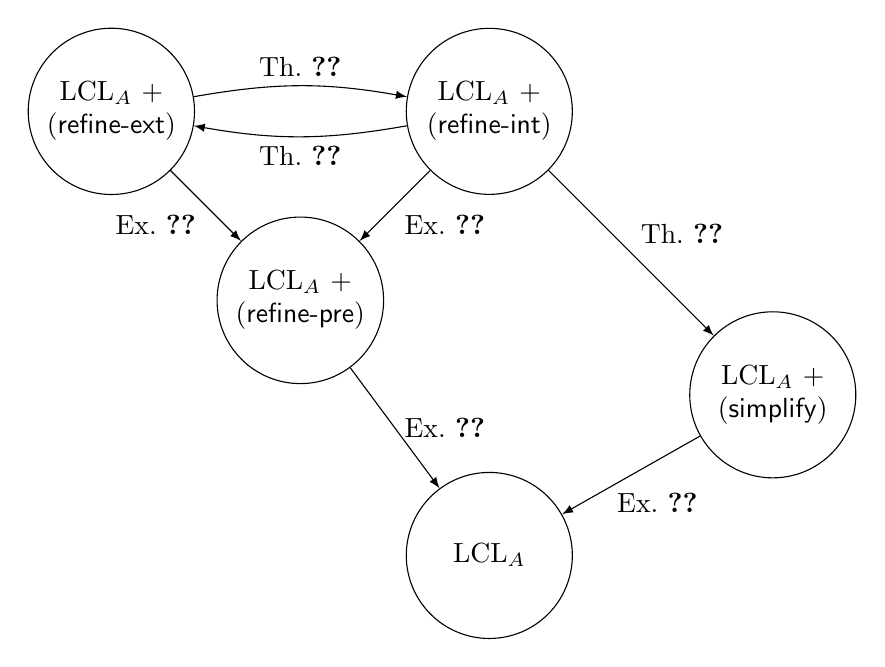
\begin{tikzpicture}[scale=1.2]
		\node[draw,circle,minimum size=6em] (LCL) at (0, -0.2) {$\LCLA$};
		\node[draw,circle,minimum size=6em,align=center] (RefPre) at (-2, 2.5) {$\LCLA$ + \\ \lclrule{refine\mbox{-}pre}};
		\node[draw,circle,minimum size=6em,align=center] (RefInt) at (0,4.5) {$\LCLA$ + \\ \lclrule{refine\mbox{-}int}};
		\node[draw,circle,minimum size=6em,align=center] (RefExt) at (-4,4.5) {$\LCLA$ + \\ \lclrule{refine\mbox{-}ext}};
		\node[draw,circle,minimum size=6em,align=center] (Simpl) at (3,1.5) {$\LCLA$ + \\ \lclrule{simplify}};

		\draw[-latex] (RefPre) edge [right] node {Ex.~\ref{ex:lcla:refine-pre-usefulness}} (LCL);
		\draw[-latex] (Simpl) edge [below right] node[shift={(-0.3,-0.1)}] {Ex.~\ref{ex:lcla:simplify-stronger}} (LCL);
		\draw[-latex] (RefExt) edge [below left] node {Ex.~\ref{ex:lcla:refine-pre-incomplete}} (RefPre);
		\draw[-latex] (RefExt) edge [bend left=10,above] node {Th.~\ref{th:lcla:refinement-rule-completeness}} (RefInt);
		\draw[-latex] (RefInt) edge [bend left=10,below] node {Th.~\ref{th:lcla:refine-int-completeness}} (RefExt);
		\draw[-latex] (RefInt) edge [below right] node {Ex.~\ref{ex:lcla:refine-pre-incomplete}} (RefPre);
		\draw[-latex] (RefInt) edge [above right] node {Th.~\ref{th:lcla:refine-int-completeness}} (Simpl);
	\end{tikzpicture}
	\caption{Relations between the new proof systems}\label{fig:lcla:rules-comparison-graph}
\end{figure}

We present a pictorial comparison among the expressiveness of the various proof systems in Figure~\ref{fig:lcla:rules-comparison-graph}. The bottom node of the diagram represents the original proof system $\LCLA$ (see Figure~\ref{fig:sota:lcla-rules}). Each other node represents the proof system extended with the single rule mentioned in the balloon. Each arrow corresponds to an expressivity result: all triples provable in the target system are also provable in the source system, which is thus more powerful. The labels of the arrows point out the result that justifies the claim. The two mutual arrows between the two topmost nodes indicate that the two proof systems are logically equivalent, i.e., they can prove the same triples. For presentation purposes, we omit arrows obtained by transitivity.

We also summarises the properties $\LCLA$ enjoys when extended with different rules in Table~\ref{tab:lcla:rules-comparison-table}.
\lclrule{refine\mbox{-}ext} is the most general refinement rule, from which the other two \lclrule{refine\mbox{-}int} and \lclrule{refine\mbox{-}pre} are derived. The former turns out to be as strong as \lclrule{refine\mbox{-}ext}, since they are both logically complete, while the latter is simpler to use, although weaker.
The only simplification rule \lclrule{simplify} is theoretically slightly stronger than plain $\LCLA$, given its intrinsic incompleteness, but it can prove triples which are not provable using \lclrule{refine\mbox{-}pre}, and it may be useful in practice.

\begin{table}[t]
	\caption{Comparison of the proof systems}
	\label{tab:lcla:rules-comparison-table}
	\centering
	\renewcommand{\arraystretch}{1.5}
	\setlength{\tabcolsep}{0.6em}
	\begin{tabular}{c|c|c}
		Proof system                          & Extensional & Logical completeness \\ \hline \hline
		Plain $\LCLA$                         & \ding{55}   & \ding{55}            \\ \hline
		$\LCLA$ + \lclrule{refine\mbox{-}ext} & \checkmark  & \checkmark           \\ \hline
		$\LCLA$ + \lclrule{refine\mbox{-}int} & \checkmark  & \checkmark           \\ \hline
		$\LCLA$ + \lclrule{refine\mbox{-}pre} & \checkmark  & \ding{55}            \\ \hline
		$\LCLA$ + \lclrule{simplify}          & \ding{55}   & \ding{55}            \\
	\end{tabular}
\end{table}

\subsection{Future works}
While the new rules we introduced are relevant from both a theoretical and practical point of view, they do not define an algorithm because of their nondeterminism:
% In principle, they may be applied to prove every triple moving to any refinement of the abstract domain, so
we need techniques to determine \emph{when} a change of abstract domain is needed and \emph{how} to choose the most convenient new domain.
We believe these two issues are actually related. For instance, if the analysis is unable to satisfy a local completeness proof obligation to apply \lclrule{transfer}, an heuristics may determine both what additional information is needed to make it true (i.e., how to refine the abstract domain) and where that additional information came from (i.e., when to refine). We briefly discussed in Section~\ref{sec:lcla:choose-refinement} some possibilities to perform this choice.
Ideally, one would systematically select an off-the-shelf abstract domain best suited to deal with each code fragment and the heuristic would inspect the proof obligations, and exploit some sort of catalogue that can track suitable abstract domains that are locally complete for the code and input at hand or derive on-the-fly some convenient domain refinement as done, e.g., by partition refinement.
To this aim, we intend to investigate a mutual exchange of ideas between CEGAR and our approach, and to integrate abstract interpretation repair into our framework.

% !TEX root = ../phd-thesis.tex

\chapter{AdjointPDR}\label{ch:pdr}
In this chapter we study a new PDR-like algorithm (see Section~\ref{sec:sota:pdr}). Differently than previous approaches, our main tool are \emph{adjunctions}, which we use extensively in our development. We propose a first algorithm, \APDR{}, which exploits an adjoint $g$ to the function $f$ (which roughly identify the backward semantics of $f$) to quicken the counterexample search. This first algorithm allows us to devise a theory of heuristics to better understand and compare them.
However, to apply \APDR{} the right adjoint $g$ to the forward semantics $f$ must exist, and this is not always the case. To get rid of this constraint, we propose \ADPDR{}, a variation of \APDR{} which lift the problem to lower sets, where it is always possible to define this adjoint.
Lastly, we propose yet another variation of the algorithm, \APDRAI{}, which can instantiate both \APDR{} and \ADPDR{}. We implemented this latter algorithm, and compared it against other PDR-like algorithms and state-of-the-art tools with encouraging results.

The content of this chapter is based on~\cite{KABBGH23}.

\section{Overview}
Category theory has recognized adjunctions $f \dashv g$ as fundamental concepts appearing across various mathematical domains~\cite{Lawvere69}. Adjointness is prevalent in various branches of computer science as well, including abstract interpretation and functional programming~\cite{Levy2004}. In our development, we employ adjoints in two distinct ways:
\begin{itemize}
	\item (Forward-Backward Adjoint) $f$ characterizes the \emph{forward semantics} of a transition system, while $g$ represents the \emph{backward} semantics.
	\item (Abstraction-Concretization Adjoint) $C$ denotes a concrete semantic domain, while $A$ is an abstract one, akin to abstract interpretation. An adjoint allows us to translate a fixed-point problem from $C$ to $A$.
\end{itemize}

The problem we address is the standard lattice-theoretical formulation of safety problems, namely whether the least fixed point of a continuous map $b$ over a complete lattice $L$ is below a given element $p \in L$: $\mu b\leq_{?} p$.

The first algorithm we present, \APDR{}, assumes the existence of an element $i \in L$ and two adjoints $f \dashv g \colon L \to L$, representing respectively initial states, forward semantics and backward semantics such that $b(x) = f(x) \lor i$ for all $x \in L$.

\[
\xymatrix{
L \ar@/_1.5ex/[r]_-{g}^-\bot &L\ar@/_1.5ex/[l]_-{f}
}
\]

Under this assumption, Knaster-Tarski Theorem~\ref{th:bg:knaster-tarski} yields the equivalences:
\[
\mu b\le p
\quad \Leftrightarrow\quad
\mu (f\lor i)\le p
\quad \Leftrightarrow\quad
i \le \nu (g \land p),
\]

where $\mu (f\lor i)$  and $\nu (g \land p)$ are, by Kleene Theorem~\ref{th:bg:kleene}, the limits of the \emph{initial} and \emph{final} chains illustrated below.
\[
\bot \le i \le f(i)\lor i \le  \cdots
\qquad\qquad\qquad
\cdots \le g(p)\land p \le p \le \top
\]

The distinguishing feature of \APDR{} is to take as a negative sequence (that is a sequential construction of potential counterexamples) an over-approximation of the final chain. This crucially differs from the negative sequence of other PDR-like algorithm, which is an under-approximation of the computed positive chain.

\APDR{} is sound (Theorem~\ref{th:pdr:soundness}) and does not loop (Proposition~\ref{prop:pdr:progres}), but since the problem $\mu b \le_? p$ is not always decidable, we cannot prove termination. Nevertheless, \APDR{} allows for a formal theory of heuristics that are essential when instantiating the algorithm to concrete problems. The theory prescribes the choices to obtain the boundary executions, using initial and final chains (Proposition~\ref{prop:pdr:negativesequencefinalchain}); it thus identifies a class of heuristics guaranteeing termination when answers are negative (Theorem~\ref{th:pdr:negativetermination}).

In general, \APDR{}'s assumption of a forward-backward adjoint $f \dashv g$ does not hold, especially in probabilistic settings. Our second algorithm \ADPDR{} circumvents this problem by extending the lattice for the negative sequence, from $L$ to the lattice $L^{\downarrow}$ of \emph{lower sets} in $L$. Specifically, by using the second form of adjoints, namely an abstraction-concretization pair, the problem $\mu b \le_{?} p$ in $L$ can be translated to an equivalent problem on $b^{\downarrow}$ in $L^\downarrow$, for which an adjoint $b^\downarrow \dashv b^\downarrow_r$ always exists.
\[
\xymatrix{
L \lloop{b} \ar@/_1.5ex/[r]_-{(-)^\downarrow}^-\bot
&L^\downarrow \rloop{b^\downarrow
	\, \dashv\, b^\downarrow_r
} \ar@/_1.5ex/[l]_-{\bigsqcup}
}
\]
This allows us to run \APDR{} in the lattice $L^\downarrow$. We then notice that the search for a positive chain can be conveniently restricted to principals in $L^\downarrow$, which have representatives in $L$. The resulting algorithm, using $L$ for positive chains and $L^\downarrow$ for negative sequences, is \ADPDR{}.

The use of lower sets for the negative sequence is a key advantage. It not only avoids the restrictive assumption of backward adjoint $g$, but also enables a more thorough search for counterexamples. {\ADPDR} can simulate stepwise LT-PDR (Theorem~\ref{th:pdr:LT-PDR-instance-ADPDR}), but it is more general since a single negative sequence in {\ADPDR} potentially represents multiple (Proposition~\ref{prop:pdr:multipleLTPDR}) or even all (Proposition~\ref{prop:pdr:LTPDRfinal}) negative sequences of LT-PDR.

Our lattice-theoretic algorithms yield many concrete instances: the original IC3/PDR as well as Reverse PDR~\cite{SS17} are instances of \APDR{} with $L$ being the powerset of the state space; since LT-PDR can be simulated by \ADPDR{}, the latter generalizes all instances in~\cite{KUKSH22}.
As a notable instance, we apply \ADPDR{} to MDPs, specifically to decide if the maximum reachability probability \cite{BK08} is below a given threshold. Here the lattice $L=[0,1]^S$ is that of fuzzy predicates over the state space $S$. Our theory provides guidance to devise two heuristics, for which we prove negative termination (Corollary~\ref{cor:pdr:ADPDRtermination}).

We implement this latter instance in Haskell. However, the implementation is not based on \ADPDR{} directly, but rather on a third algorithm, \APDRAI{}. This can be understood as a generalisation of both \APDR{} and \ADPDR{} to a more abstract setting:
\[
\xymatrix{
(L, \le_L) \lloop{b} \ar[r]^-{\gamma}
&(C, \le_C) \rloop{\overline{b} \dashv \overline{b}_r}
}
\]
where $\gamma \colon L \to C$ is an order embedding and $b,\overline{b}$ and $\gamma$ are required to satisfy a condition that is known in the setting of abstract interpretation as \emph{forward completeness}~\cite{GRS00}.

We experimentally evaluate our implementation. We compare it against existing probabilistic PDR algorithms (PrIC3~\cite{BJKKMS20}, LT-PDR~\cite{KUKSH22}) and a non-PDR one (Storm~\cite{DJKV17}). The performance of \ADPDR{} is encouraging---it supports the potential of PDR algorithms in probabilistic model checking. The experiments also indicate the importance of having a variety of heuristics, and thus the value of our adjoint framework that helps in coming up with those.
Additionally, we found that abstraction features of Haskell allow us to code lattice-theoretic algorithms almost literally ($\sim$100 lines). Implementing a few heuristics takes another $\sim$240 lines. This way, we found that mathematical abstraction can directly help in easing implementation effort.

\section{Adjoint PDR}\label{sec:pdr:APDR}

\begin{figure}[t]
	% Syntactic invariants
	\begin{minipage}{.35\linewidth}
		\small
		\begin{align}
			\quad x_0 = \bot \tag{I0}\label{eq:pdr:x0bot} \\
			1\leq k \leq n \tag{I1} \label{eq:pdr:invi}   \\
			\forall j\in[0, n-2]\text{, }x_j \le x_{j+1} \tag{I2}\label{eq:pdr:positivechain}
		\end{align}
	\end{minipage}%
	% General invariants
	\begin{minipage}{.65\linewidth}
		\small
		\begin{align}
			\forall j \in [k, n - 1] \text{, } x_j \not\le y_j \tag{PN} \label{eq:pdr:positivenegative}                                              \\
			\forall j \in [0, n-1] \text{, } (f \lor i)^j (\bot) \le x_j \le (g \land p)^{n-1-j} (\top) \tag{A1} \label{eq:pdr:positiveinitialfinal} \\
			\forall j \in [1, n-1] \text{, } x_{j-1} \le g^{n-1-j}(p) \tag{A2} \label{eq:pdr:positivefinal}                                          \\
			\forall j\in[k,n-1]\text{, }g^{n-1-j}(p) \le y_j \tag{A3} \label{eq:pdr:negativefinal}
		\end{align}
	\end{minipage}
	% Positive chain invariants
	\begin{minipage}{.4\linewidth}
		\small
		\begin{align}
			i \le x_1 \tag{P1} \label{eq:pdr:Ix1}                                            \\
			x_{n-2} \le p \tag{P2}\label{eq:pdr:xP}                                          \\
			\forall j\in[0, n-2]\text{, }f(x_j) \le x_{j+1} \tag{P3}\label{eq:pdr:positiveF} \\
			\forall j\in[0, n-2]\text{, }x_j \le g(x_{j+1}) \tag{P3a} \label{eq:pdr:positiveG}
		\end{align}
	\end{minipage}%
	% Negative sequence invariants
	\begin{minipage}{.6\linewidth}
		\small
		\begin{align}
			\text{If }\vec{y}\neq \varepsilon\text{ then }p \le y_{n-1} \tag{N1}\label{eq:pdr:Pepsilon} \\
			\forall j\in[k,n-2]\text{, }g(y_{j+1}) \le y_j \tag{N2}\label{eq:pdr:negativeG}
		\end{align}
	\end{minipage}

	\vspace*{0.5em}
	\caption{Invariants of {\APDR}.}
	\label{fig:pdr:invariants}
\end{figure}

In this section we introduce {\APDR}, an algorithm that takes in input a tuple $(i,f,g,p)$ with $i,p\in L$ and $f\dashv g \colon L\to L$ and, if it terminates, it returns true whenever $\lfp (f \lor i) \le p$ and false otherwise. The algorithm manipulates two sequences of elements of $L$:
\[
\vec{x} \eqdef x_0, \dots, x_{n-1} \qquad \vec{y} \eqdef y_k, \dots y_{n-1}
\]
of length $n$ and $n-k$, respectively. These satisfy, through the executions of {\APDR}, the invariants in Figure~\ref{fig:pdr:invariants}. By \eqref{eq:pdr:positiveinitialfinal}, $x_j$ over-approximates the $j$-th element of the initial chain, namely $(f \lor i)^j(\bot) \le x_j$, while, by \eqref{eq:pdr:negativefinal}, the $j$-indexed element $y_j$ of $\vec{y}$ over-approximates $g^{n-j-1}(p)$ that, borrowing the terminology of Example~\ref{ex:sota:ts}, is the set of states which are safe in $n-j-1$ transitions.
Moreover, by~\eqref{eq:pdr:positivenegative}, the element $y_j$ witnesses that $x_j$ is unsafe, i.e., that $x_j \nleq g^{n-1-j}(p)$ or equivalently $f^{n-j-1}(x_j) \nleq p$.
Notably, $\vec{x}$ is a positive chain and $\vec{y}$ a negative sequence, according to the definitions below.

\begin{definition}[positive chain] \label{def:pdr:posi_seq}
	A \emph{positive chain} for $\lfp (f \lor i) \le p$ is a finite chain $x_0 \le \dots \le x_{n-1}$ in $L$ of length $n \geq 2$ which satisfies \eqref{eq:pdr:Ix1}, \eqref{eq:pdr:xP}, \eqref{eq:pdr:positiveF} in Figure~\ref{fig:pdr:invariants}.
	It is \emph{conclusive} if $x_{j+1} \le x_j$ for some $j \leq n-2$.
\end{definition}

In a conclusive positive chain, $x_{j+1}$ provides an invariant for $f \lor i$ and thus, by \eqref{eq:bg:coinductionproofprinciple}, $\lfp (f \lor i) \le p$ holds. So, when $\vec{x}$ is conclusive, {\APDR} returns true.

\begin{definition}[negative sequence] \label{def:pdr:neg_seq}
	A \emph{negative sequence} for $\lfp (f \lor i) \le p$ is a finite sequence $ y_k, \dots, y_{n-1}$ in $L$ with $1 \leq k \leq n$ which satisfies \eqref{eq:pdr:Pepsilon} and \eqref{eq:pdr:negativeG} in Figure~\ref{fig:pdr:invariants}.
	It is \emph{conclusive} if $k=1$ and $i \nleq y_1$.
\end{definition}

When $\vec{y}$ is conclusive, {\APDR} returns false as $y_1$ provides a counterexample: \eqref{eq:pdr:Pepsilon} and \eqref{eq:pdr:negativeG} entail \eqref{eq:pdr:negativefinal} and thus $i \nleq y_1 \ge g^{n-2}(p)$, so that $g^{n-2}(p) \ge \gfp (g \land p)$ and thus $i \nleq \gfp(g \land p)$. By~\eqref{eq:bg:adjoint-fixpoint}, $\lfp(f \lor i) \nleq p$.

\begin{figure}[t]
	\begin{center}
		\underline{{\APDR} $(i,f,g,p)$}
		{\small
			\begin{codeNT}
<INITIALISATION>
  $( \vec{x} \| \vec{y} )_{n,k}$ := $(\bot,\top\|\varepsilon)_{2,2}$
<ITERATION>						           % $\vec{x},\vec{y}$  not conclusive
  case $( \vec{x} \| \vec{y} )_{n,k}$ of
	   $\vec{y}=\varepsilon$ And $x_{n-1} \le p$     :                    %(Unfold)
			$( \vec{x} \| \vec{y} )_{n,k}$ := $( \vec{x}, \top \| \varepsilon )_{n+1,n+1}$
	   $\vec{y}=\varepsilon$ And $x_{n-1} \not\le p$    :                     %(Candidate)
			choose $z\in L$ st  $x_{n-1} \not\le z$ And  $p \le z$;
			$( \vec{x} \| \vec{y} )_{n,k}$ := $( \vec{x} \| z )_{n,n-1}$
	   $\vec{y} \neq \varepsilon$ And $f(x_{k-1}) \not \le y_k$ :                        %(Decide)
			choose $z \in L$ st $x_{k-1} \not \le z$ And $g(y_k) \le z$;
			$(\vec{x} \| \vec{y} )_{n,k}$ := $(\vec{x} \| z , \vec{y} )_{n,k-1}$
	   $\vec{y} \neq \varepsilon$ And $f(x_{k-1}) \le y_k$ :                        %(Conflict)
			choose $z \in L$ st $z \le y_k$ And $(f \lor i)(x_{k-1} \land z) \le z$;
			$(\vec{x} \| \vec{y} )_{n,k}$ := $(\vec{x} \land_k z \| \mathsf{tail}(\vec{y}) )_{n,k+1}$
  endcase
<TERMINATION>
	if $\exists j\in [0,n-2]\,.\, x_{j+1} \le x_j$ then return true		 % $\vec{x}$ conclusive
	if $i \not \le y_1$ then return false							% $\vec{y}$ conclusive
\end{codeNT}
		}
	\end{center}
	\caption{{\APDR} algorithm checking $\lfp(f \lor i) \le p$.}\label{fig:pdr:apdr}
\end{figure}

The pseudocode of the algorithm is in Figure~\ref{fig:pdr:apdr}, where we write $( \vec{x} \| \vec{y} )_{n,k}$ to compactly represents the state of the algorithm: the pair $(n,k)$ is called the \emph{index} of the state, with $\vec{x}$ of length $n$ and $\vec{y}$ of length $n-k$. When $k = n$, $\vec{y}$ is the empty sequence $\varepsilon$. For any $z \in L$, we write $\vec{x}, z$ for the chain $x_0, \dots, x_{n-1}, z$ of length $n+1$ and $z, \vec{y}$ for the sequence $z, y_k, \dots y_{n-1}$ of length $n-(k-1)$. Moreover, we write $\vec{x} \land_j z$ for the chain $x_0 \land z, \dots, x_j \land z, x_{j+1}, \dots , x_{n-1}$. Finally, $\mathsf{tail}(\vec{y})$ stands for the tail of $\vec{y}$, namely $y_{k+1}, \dots y_{n-1}$ of length $n-(k+1)$.

The algorithm starts in the initial state $s_0 \eqdef ( \bot, \top \| \varepsilon )_{2,2}$ and, unless one of $\vec{x}$ and $\vec{y}$ is conclusive, iteratively applies one of the four mutually exclusive rules: (Unfold), (Candidate), (Decide) and (Conflict).
The rule (Unfold) extends the positive chain by one element when the negative sequence is empty and the positive chain is under $p$; since the element introduced by (Unfold) is $\top$, its application typically triggers rule (Candidate) that starts the negative sequence with an over-approximation of $p$. Recall that the role of $y_j$ is to witness that $x_j$ is unsafe. After (Candidate) either (Decide) or (Conflict) are possible: if $y_k$ witnesses that, besides $x_k$, also $f(x_{k-1})$ is unsafe, then (Decide) is used to further extend the negative sequence to witness that $x_{k-1}$ is unsafe; otherwise, the rule (Conflict) improves the precision of the positive chain in such a way that $y_k$ no longer witnesses $x_k \land z$ unsafe and, thus, the negative sequence is shortened.
Note that, in (Candidate), (Decide) and (Conflict), the element $z \in L$ is chosen among a set of possibilities, thus {\APDR} is nondeterministic.

To illustrate the executions of the algorithm, we adopt a labeled transition system notation. Let $\states \eqdef \{( \vec{x} \| \vec{y} )_{n,k} \mid n \geq 2$, $k\leq n$, $\vec{x}\in L^n$ and $\vec{y}\in L^{n-k}\}$ be the set of all possible states of {\APDR}. We call $( \vec{x} \| \vec{y} )_{n,k} \in \states$ \emph{conclusive} if $\vec{x}$ or $\vec{y}$ are such.
When $s \in \states$ is not conclusive, we write $s \trz{D}{}$ to mean that $s$ satisfies the guards in the rule (Decide), and $s \trz{D}{z} s'$ to mean that, being (Decide) applicable, {\APDR} moves from state $s$ to $s'$ by choosing $z$. Similarly for the other rules: the labels $\mathit{Ca}$, $\mathit{Co}$ and $U$ stands for (Candidate), (Conflict) and (Unfold), respectively.
When irrelevant we omit to specify labels and choices and we just write $s \tr{} s'$.
As usual $\ttp{}$ stands for the transitive closure of $\tr{}$ and $\ttr{}$ stands for the reflexive and transitive closure of $\tr{}$.

\begin{example}\label{ex:pdr:simple-ts}
	Consider the safety problem in Example~\ref{ex:sota:ts}. Below we illustrate two possible computations of {\APDR} that differ for the choice of $z$ in (Conflict).
	The first run is conveniently represented as the following series of transitions.
	\par\nobreak
	{
		\setlength{\abovedisplayskip}{0pt}
		\setlength{\belowdisplayskip}{6pt}
		\setlength{\abovedisplayshortskip}{0pt}
		\setlength{\belowdisplayshortskip}{3pt}
		\begin{align*}
			                     & ( \emptyset, S \| \varepsilon )_{2,2}
			\tr{\mathit{Ca}}_{P} ( \emptyset, S \| P )_{2,1}
			\tr{\mathit{Co}}_{I} ( \emptyset, I \| \varepsilon )_{2,2}                  \\[-.4em]
			\tr{U}               & ( \emptyset, I, S \| \varepsilon )_{3,3}
			\tr{\mathit{Ca}}_{P} ( \emptyset, I, S \| P )_{3,2}
			\tr{\mathit{Co}}_{S_2} ( \emptyset, I, S_2 \| \varepsilon )_{3,3}           \\[-.4em]
			\tr{U} %
			\tr{\mathit{Ca}}_{P} & ( \emptyset, I, S_2, S \| P )_{4,3}
			\tr{\mathit{Co}}_{S_3} ( \emptyset, I, S_2, S_3 \| \varepsilon )_{4,4}      \\[-.4em]
			\tr{U} %
			\tr{\mathit{Ca}}_{P} & ( \emptyset, I, S_2, S_3, S \| P )_{5,4}
			\tr{\mathit{Co}}_{S_4} ( \emptyset, I, S_2, S_3, S_4 \| \varepsilon )_{5,5} \\[-.4em]
			\tr{U} %
			\tr{\mathit{Ca}}_{P} & ( \emptyset, I, S_2, S_3, S_4, S \| P )_{6,5}
			\tr{\mathit{Co}}_{S_4} ( \emptyset, I, S_2, S_3, S_4, S_4 \| \varepsilon )_{6,6}
		\end{align*}
	}

	\noindent
	The last state returns true since $x_4 = x_5 = S_4$. Observe that the chain $\vec{x}$, with the exception of its last element $x_{n-1}$, is exactly the initial chain of $(T \cup I)$, i.e., $x_j$ is the set of states reachable in at most $j-1$ steps. In the second computation, the elements of $\vec{x}$ are roughly those of the final chain of $(G \cap P)$. More precisely, after (Unfold) or (Candidate), $x_{n-j}$ for $j < n-1$ is the set of states which only reach safe states within $j$ steps.
	\par\nobreak
	{
		\setlength{\abovedisplayskip}{0pt}
		\setlength{\belowdisplayskip}{6pt}
		\setlength{\abovedisplayshortskip}{0pt}
		\setlength{\belowdisplayshortskip}{3pt}
		\begin{align*}
			                     & ( \emptyset, S \| \varepsilon )_{2,2}
			\tr{\mathit{Ca}}_{P} ( \emptyset, S \| P )_{2,1}
			\tr{\mathit{Co}}_{P} ( \emptyset, P \| \varepsilon )_{2,2}      \\[-.4em]
			\tr{U} %
			\tr{\mathit{Ca}}_{P} & ( \emptyset, P, S \| P )_{3,2}
			\tr{D}_{S_4} ( \emptyset, P, S \| S_4, P )_{3,1}
			\tr{\mathit{Co}}_{S_4} ( \emptyset, S_4, S \| P )_{3,2}
			\tr{\mathit{Co}}_{P} ( \emptyset, S_4, P \| \varepsilon )_{3,3} \\[-.4em]
			\tr{U} %
			\tr{\mathit{Ca}}_{P} & ( \emptyset, S_4, P, S \| P )_{4,3}
			\tr{D}_{S_4} ( \emptyset, S_4, P, S \| S_4, P )_{4,2}
			\tr{\mathit{Co}}_{S_4} ( \emptyset, S_4, S_4, S \| P )_{4,3}
		\end{align*}
	}

	\noindent
	Observe that, by invariant \eqref{eq:pdr:positiveinitialfinal}, the values of $\vec{x}$ in the two runs are, respectively, the least and the greatest values for all possible computations of {\APDR}.
\end{example}

\section{Properties of {\APDR}}\label{sec:pdr:properties}

In this section we prove the main properties of {\APDR}: (1) any returned result is valid (soundness); (2) although {\APDR} can diverge, any state is never visited twice (called progression); (3) certain heuristics can be used to guarantee termination when a counterexample exists (called negative termination).

\subsection{Invariants}\label{sec:pdr:soundness}
The proofs of the properties of {\APDR} rely on the properties in Figure~\ref{fig:pdr:invariants}. In this section, we prove that such properties are invariants:
\begin{prop}\label{prop:pdr:invariants-valid}
	For any possible choice performed by {\APDR}, the properties in Figure~\ref{fig:pdr:invariants} hold in all reachable states of the algorithm.
\end{prop}

In proving the invariants, some observations on the choice of element $z$ naturally emerge.
First, the proofs of the three invariants \eqref{eq:pdr:x0bot}, \eqref{eq:pdr:invi} and \eqref{eq:pdr:positivechain} do not rely on the properties of the chosen element $z \in L$.
For proving the invariants of the positive chain (\eqref{eq:pdr:Ix1}, \eqref{eq:pdr:xP}, \eqref{eq:pdr:positiveF} and \eqref{eq:pdr:positiveG}) and of the negative sequence (\eqref{eq:pdr:Pepsilon} and \eqref{eq:pdr:negativeG}) we only exploit the \emph{second} constraints on $z$ of each rule of the algorithm, namely $p \le z$ in (Candidate), $g(y_k) \le z$ in (Decide), and $(f \lor i)(x_{k-1} \land z) \le z$ in (Conflict).
Lastly, the \emph{first} constraint on $z$ in each rule ensures the remaining invariants (\eqref{eq:pdr:positivenegative}, \eqref{eq:pdr:positiveinitialfinal}, \eqref{eq:pdr:positivefinal} and \eqref{eq:pdr:negativefinal}), which in turn are key to the proof of progression.

To make the proofs more uniform and compact, we adopt the following notation: for a state $s$ and a property $(Q)$ we will write $s \models (Q)$ to mean that $(Q)$ holds in $s$. We will often show that $(Q)$ is an invariant inductively: namely, we will prove
\begin{itemize}
	\item[(a)] $s_0 \models (Q)$ and
	\item[(b)] if $s \models (Q)$ and $s \tr{ } s'$, then $s'\models (Q)$.
\end{itemize}
Hereafter, we fix $s=( \vec{x} \| \vec{y} )_{n,k}$ and $s'=( \vec{x}' \| \vec{y}' )_{n',k'}$. As usual we will write $x_j$ and $y_j$ for the elements of $\vec{x}$ and $\vec{y}$. For the elements of $\vec{x}'$ and $\vec{y}'$, we will write $x_j'$ and $y_j'$. Throughout the proofs, we will avoid to repeat every time in (b) that $s \models (Q)$, and we will just write $\stackrel{{(Q)}}{=}$ or $\stackrel{{(Q)}}{{\le}}$ whenever using such hypothesis. Moreover in (b) we will avoid to specify those cases that are trivial: for instance, for the properties that only concerns the positive chain $\vec{x}$, e.g., \eqref{eq:pdr:x0bot} and \eqref{eq:pdr:positiveF}, it is enough to check the property (b) for $s \tr{U} s'$ and $s \tr{\mathit{Co}} s'$, since $s \tr{D} s'$ and $s \tr{\mathit{Ca}} s'$ only modify the negative sequence $\vec{y}$.
We illustrate below only the most interesting cases. The remaining ones are in Appendix~\ref{ch:app:pdr}.

\begin{proof}[Proof sketch]
	\invariantproof{\eqref{eq:pdr:x0bot}}{$x_0 = \bot$}
	\begin{itemize}
		\item[(a)] In $s_0$, $x_0= \bot$.
		\item[(b)] If $s \tr{U} s'$, then $x_0' = x_0 \stackrel{{\eqref{eq:pdr:x0bot}}}{=}\bot$. \\
		      If $s \trz{\mathit{Co}}{z} s'$, then $x_0'=x_0 \land z \stackrel{{\eqref{eq:pdr:x0bot}}}{=} \bot \land z = \bot$.
	\end{itemize}

	\invariantproof{\eqref{eq:pdr:invi}}{$1\leq k \leq n$}
	\begin{itemize}
		\item To prove that $1 \leq k$, observe that $k$ is initialised at $2$ and that it is only decremented by $1$. When $k=1$, $\vec{y}\neq \varepsilon$. By~\eqref{eq:pdr:x0bot} $x_0=\bot$. Since $f$ is a left adjoint, $f(\bot) = \bot$. Thus, $f(x_0) \le y_1$. This means that either the state is conclusive and the algorithm returns, or (Conflict) is enabled and thus $k$ is incremented.
		\item To prove that $k \leq n$, observe that $k$ is incremented only by $1$. When $k=n$, the algorithm does either (Unfold) or (Candidate). In the latter case, $k$ is decremented. In the former, both $n$ and $k$ are incremented.
	\end{itemize}

	\invariantproof{\eqref{eq:pdr:positiveF}}{$\forall j\in[0, n-2] \text{, } f(x_j) \le x_{j+1}$}
	\begin{itemize}
		\item[(a)] In $s_0$, since $n=2$ one needs to check only the case $j=0$: $f(x_0) \le \top = x_1$.
		\item[(b)] If $s \tr{U} s'$, then $f(x_j') =f(x_j) \stackrel{{\eqref{eq:pdr:positivechain}}}{\le} x_{j+1} =x_{j+1}'$ for all $j\in[0,n-2]$. For $j=n-1$, $f(x_{n-1}') = f(x_{n-1}) \le \top = x_{j+1}'$. Since $n'=n+1$, then $\forall j\in [0,n'-2] \text{, } f(x_j')\le x_{j+1}'$. \\
		      If $s \trz{\mathit{Co}}{z} s'$, since $f(x_{k-1} \land z) \le z$, then by \eqref{eq:pdr:positivechain} and monotonicity of $f$ it holds that $\forall j\in [0,k-1]$, $f(x_{j} \land z) \le z$. Since $f(x_j \land z) \le f(x_j) \stackrel{{\eqref{eq:pdr:positiveF}}}{\le} x_{j+1}$, it holds that $f(x_j \land z) \le x_{j+1} \land z $ for all $j\in[0, k-1]$. With this observation is immediate to conclude that $\forall j\in[0,n'-2] \text{, }f(x_j')\le x_{j+1}'$.
	\end{itemize}

	\invariantproof{\eqref{eq:pdr:negativeG}}{$\forall j\in[k,n-2] \text{, } g(y_{j+1}) \le y_j$}\newline
	The case of (Conflict) is trivial: the negative sequence $\vec{y}$ is truncated in the rule (Conflict), and if the invariant holds for $\vec{y}$ then it holds for its tail $\mathsf{tail}(\vec{y})$ as well.
	\begin{itemize}
		\item[(a)] In $s_0$, $k=2$ and $n=2$. Thus \eqref{eq:pdr:negativeG} trivially holds.
		\item[(b)] If $s \tr{\mathit{Ca}} s'$, then $k'=n-1$ and thus \eqref{eq:pdr:negativeG} trivially holds.\\
		      If $s \trz{D}{z} s'$, since $z \ge g(y_k)$ and $k'=k-1$, then $y_{k'}' = y_{k-1}' = z \ge g(y_k) = g(y_k')= g(y_{k'+1}')$. For $j\in[k'+1,n-2]$, namely for $j\in[k,n-2]$, it holds that $y'_j= y_j\stackrel{{\eqref{eq:pdr:negativeG}}}{\ge} g(y_{j+1})=g(y_{j+1}')$. Thus, $\forall j \in [k',n-2] \text{, }g(y_{j+1}') \le y_j'$.
	\end{itemize}

	\invariantproof{\eqref{eq:pdr:positivenegative}}{$\forall j \in [k, n - 1] \text{, } x_j \not\le y_j$}
	\begin{itemize}
		\item[(a)] In $s_0$, $k=n$ and thus \eqref{eq:pdr:positivenegative} trivially holds.
		\item[(b)] If $s \tr{U} s'$, then $k'=n'$ and thus \eqref{eq:pdr:positivenegative} trivially holds.\\
		      If $s \trz{\mathit{Ca}}{z} s'$, since $x_{n-1} \not\le z$, $x'_{n-1}=x_{n-1}$ and $k'=n'-1=n-1$, then $x'_{n'-1} = x_{n-1}\not\le z = y'_{n'-1}$. \\
		      If $s \trz{D}{z} s'$, since $x_{k-1} \not\le z$, then $x_{k-1}'=x_{k-1} \not\le z = y'_{k-1}$. Moreover, $\forall j \in [k, n - 1]$,
		      $x_j' = x_j \stackrel{{\eqref{eq:pdr:positivenegative}}}{ \not\le} y_j = y_j'$. Thus, $\forall j \in [k', n' - 1] \text{, } x_j' \not\le y_j'$.\\
		      If $s \tr{\mathit{Co}} s'$, then $k'=k+1$ and $n'=n$. Observe that for $j \in [k + 1, n - 1]$, $x'_j = x_j \stackrel{{\eqref{eq:pdr:positivenegative}}}{ \not\le} y_j =y_j'$. Thus $\forall j \in [k', n' - 1] \text{, }x_j' \not\le y_j' $.
	\end{itemize}
\end{proof}

\subsection{Soundness}

Once the properties in Figure~\ref{fig:pdr:invariants} are proved to be invariants, the proof of soundness of {\APDR} is rather straightforward: it only appeals to the Knaster-Tarski fixed-point theorem for the positive case, and to the Kleene one for the negative case.

\begin{theorem}[Soundness]\label{th:pdr:soundness}
	\emph {\APDR} is sound, namely,
	\begin{enumerate}
		\item If \emph{\APDR} returns true then $\lfp (f \lor i) \le p$.
		\item If \emph{\APDR} returns false then $\lfp (f \lor i) \nleq p$.
	\end{enumerate}
\end{theorem}
\begin{proof}
	We prove the two items separately.
	\begin{enumerate}
		\item Observe that {\APDR} returns true if $x_{j+1} \le x_j$. By \eqref{eq:pdr:positiveF}, we thus have $f(x_j) \le x_{j+1} \le x_j$. Moreover, by \eqref{eq:pdr:Ix1} and \eqref{eq:pdr:positivechain}, it holds that $i \le x_j$ and $x_j \le p$. Therefore, it holds that
		      \[
		      (f \lor i) x_j \le x_j \le p \text{.}
		      \]
		      By \eqref{eq:bg:coinductionproofprinciple}, we have that $\lfp (f \lor i) \le p$.
		\item Observe that {\APDR} returns false if $i \nleq y_1$. By \eqref{eq:pdr:negativefinal}, $g^{n-2}(p) \le y_1$. Thus $i \nleq g^{n-2}(p)$. Moreover
		      \begin{align*}
			      g^{n-2}p & \le \bigwedge_{j\in \omega} g^{j}(p) \\
			               & = \gfp (g \land p)
		      \end{align*}
		      Thus $i \nleq \gfp(g \land p) $. By \eqref{eq:bg:adjoint-fixpoint}, $\lfp(f \lor i) \nleq p$.
	\end{enumerate}
\end{proof}

\subsection{Progression}\label{sec:pdr:progression}
It is necessary to prove that in any step of the execution, if the algorithm does not return true or false, then it can progress to a new state, not yet visited. To this aim we must deal with the subtleties of the non-deterministic choice of the element $z$ in (Candidate), (Decide) and (Conflict). The following proposition ensures that, for any of these three rules, there is always a possible choice.

\begin{prop}[Canonical choices]\label{prop:pdr:CanonicalChoice}
	The following choices of $z$ are always possible:
	\begin{enumerate}
		\item in (Candidate) $z=p$;
		\item in (Decide) $z= g(y_k)$;
		\item in (Conflict) $z = y_k$;
		\item in (Conflict) $z = (f \lor i)(x_{k-1})$.
	\end{enumerate}
	Thus, for all non-conclusive $s\in \states$, if $s_0 \ttr{} s $ then $s \tr{}$.
\end{prop}
\begin{proof}
	For each rule, we prove that if the guard of the rule is satisfied then the choice of $z$ satisfies the required constraints.
	\begin{enumerate}
		\item The guard of (Candidate) is $x_{n-1} \not\le p$. By choosing $z=p$, one has that $x_{n-1} \not \le z$ and $p \le z$ are trivially satisfied;
		\item The guard of (Decide) is $f(x_{k-1}) \not\le y_k$ thus, by $f \dashv g$, $x_{k-1} \not \le g(y_k)$. By choosing $z= g(y_k)$, one has that $x_{k-1} \not\le z$ and $g(y_k) \le z$;
	\end{enumerate}
	The proofs for the choices in (Conflict) are more subtle. First of all, observe that if $k=1$, then $i\le y_1$ otherwise the algorithm would have returned false. Moreover, for $k\geq 2$, we have that
	$i \le x_{k-1} \le y_k$: the first inequality holds by \eqref{eq:pdr:Ix1} and the second by \eqref{eq:pdr:positivefinal} and \eqref{eq:pdr:negativefinal}. In summary,
	\begin{equation}\label{eq:pdr:yigeqI}
		\forall j \geq 1 \sdot i \le y_j \text{.}
	\end{equation}
	We can then proceed as follows.
	\begin{enumerate}\setcounter{enumi}{2}
		\item The guard of (Conflict) is $f(x_{k-1}) \le y_k$. By choosing $z=y_k$, one has that $z \le y_k$ trivially holds. For $(f \lor i)(x_{k-1} \land z) \le z$ observe that
		      \begin{align*}
			      (f \lor i)(x_{k-1} \land z) & = f(x_{k-1} \land z) \lor i & [\text{def.}]           \\
			                                  & \le f(x_{k-1} ) \lor i      & [\text{monotonicity}]   \\
			                                  & \le z \lor i                & [\text{guard}]          \\
			                                  & = z                         & [\eqref{eq:pdr:yigeqI}]
		      \end{align*}

		\item The guard of (Conflict) is $f(x_{k-1}) \le y_k$. By choosing $z=(f \lor i)(x_{k-1})$, one has that $(f \lor i)(x_{k-1} \land z) \le (f \lor i)(x_{k-1}) =z$ holds by monotonicity.
		      For $z \le y_k$, by using the guard and \eqref{eq:pdr:yigeqI}, we have that $z= (f \lor i)(x_{k-1}) = f(x_{k-1}) \lor i \le y_k$.
	\end{enumerate}
\end{proof}

The following proposition ensures that {\APDR} always traverses new states.
\begin{prop}[Impossibility of loops]\label{prop:pdr:progres}
	If $s_0 \ttr{} s \ttp{ } s'$, then $s\neq s'$.
\end{prop}
\begin{proof}
	Let us consider the following partial order on positive chains: given two sequences $\vec{x}= x_0, \dots x_{n-1}$ and $\vec{x}' = x'_0, \dots, x'_{n'-1}$, we say $\vec{x} \preceq \vec{x}'$ if
	\begin{equation*}
		n \le n' \land x_j \ge x'_j \text{ for each } j\in[0,n - 1]
	\end{equation*}
	We extend the order to states by letting $(\vec{x} \| \vec{y} )_{n, k} \preceq (\vec{x}' \| \vec{y}' )_{n', k'}$ with $\vec{x} \prec \vec{x}'$ or $\vec{x} = \vec{x}'$ and $k \ge k'$.

	We prove the statement by showing that applying a rule strictly increases the state in that partial order.
	As before, we use non-primed variables such as $\vec{x}$ for values before the application of a rule, and primed variables such as $\vec{x}'$ after.

	For (Unfold), we have that $n < n' = n + 1$ and $x_j = x'_j$ for each $j\in[0,n - 1]$.

	For (Candidate), we have $\vec{x}' = \vec{x}$ and $k' = n - 1 < n = k$.

	For (Decide), we have $\vec{x}' = \vec{x}$ and $k' = k - 1 < k$.

	For (Conflict), $n = n'$, and
	\[
	x'_j = \begin{cases*}
		x_j         & if $j > k$   \\
		x_j \land z & if $j \le k$
	\end{cases*}
	\]
	So for $j\in[k+1,n - 1]$ we have $x_j = x'_j$, and for $j\in[0,k]$ we have $x_j \ge x_j \land z = x'_j$. So $\vec{x} \preceq \vec{x}'$. Assume by contradiction that $x'_k = x_k$. Since $x'_k = x_k \land z$, this is equivalent to $x_k \le z$. The choice of $z$ in (Conflict) satisfies $z \le y_k$, that would imply $x_k \le z \le y_k$. However, this is a contradiction, since by \eqref{eq:pdr:positivenegative} we know $x_k \not \le y_k$. Hence $x_k \ge x'_k$, meaning $\vec{x} \prec \vec{x}'$.
\end{proof}

Observe that the above propositions entail that {\APDR} terminates whenever the lattice $L$ is finite, since the set of reachable states is finite in this case.

\begin{example}
	For $(I,T,G,P)$ as in Example~\ref{ex:sota:ts}, {\APDR} behaves essentially as IC3/PDR~\cite{Bradley11}, solving reachability problems for transition systems with finite state space $S$. Since the lattice $\mathcal{P}S$ is also finite, {\APDR} always terminates.
\end{example}

\subsection{Heuristics}\label{sec:pdr:heuristics}
The nondeterministic choices of the algorithm can be resolved by using heuristics. Intuitively, a heuristic chooses for any states $s\in\states$ an element $z\in L$ to be possibly used in (Candidate), (Decide) or (Conflict), so it is just a function $h\colon \states \to L$.
When defining a heuristic, we will avoid to specify its values on conclusive states or in those performing (Unfold), as they are clearly irrelevant.

With a heuristic, one can instantiate {\APDR} by making the choice of $z$ as prescribed by $h$. Syntactically, this means to erase from the code of Figure~\ref{fig:pdr:apdr} the three lines of \texttt{choose} and replace them with $z \texttt{:= } h(\,( \vec{x} \| \vec{c} )_{n,k}\,)$. We call {\APDR}$_h$ the resulting deterministic algorithm and write $s \Htrz{}{h}{} s'$ to mean that {\APDR}$_h$ moves from state $s$ to $s'$. We let $\states^h \eqdef \{s\in \states \mid s_0\Htrz{}{h}{*} s\}$ be the sets of all states reachable by {\APDR}$_h$.

\begin{definition}[legit heuristic]
	A heuristic $h\colon \states \to L$ is called \emph{legit} whenever for all $s,s'\in \states^h$, if $s \Htrz{}{h}{}s'$ then $s\tr{}s'$.
\end{definition}
When $h$ is legit, the only execution of the deterministic algorithm {\APDR}$_h$ is one of the possible executions of the non-deterministic algorithm {\APDR}.

The canonical choices provide two legit heuristics: first, we call \emph{simple} any legit heuristic $h$ that chooses $z$ in (Candidate) and (Decide) as in Proposition \ref{prop:pdr:CanonicalChoice}:
\begin{equation}\label{eq:pdr:simple}
	( \vec{x} \| \vec{y} )_{n,k} \mapsto
	\begin{cases*}
		p      & if $( \vec{x} \| \vec{y} )_{n,k} \tr{ \mathit{Ca} }$ \\
		g(y_k) & if $( \vec{x} \| \vec{y} )_{n,k} \tr{ D }$
	\end{cases*}
\end{equation}
Then, if the choice in (Conflict) is like in Proposition \ref{prop:pdr:CanonicalChoice}.4, we call $h$ \emph{initial}; if it is like in Proposition \ref{prop:pdr:CanonicalChoice}.3, we call $h$ \emph{final}. Shortly, the two legit heuristics are:
\[
\begin{array}{r|ll}
	\quad\emph{simple initial} \quad\
	                   & \quad\eqref{eq:pdr:simple} \text{ and }( \vec{x} \| \vec{y} )_{n,k} \mapsto
	(f\lor i)(x_{k-1}) & \quad\mbox{if $( \vec{x} \| \vec{y} )_{n,k} \in \mathit{Co}$}\quad
	\\[5pt]
	\hline
	\\[-7pt]
	\quad\emph{simple final} \quad\
	                   & \quad\eqref{eq:pdr:simple} \text{ and }
	( \vec{x} \| \vec{y} )_{n,k} \mapsto
	y_k                & \quad\mbox{if $( \vec{x} \| \vec{y} )_{n,k} \in \mathit{Co}$}\quad          \\
\end{array}
\]
Interestingly, with any simple heuristic, the sequence $\vec{y}$ takes a familiar shape:
\begin{prop}\label{prop:pdr:negativesequencefinalchain}
	Let $h\colon \states \to L$ be any simple heuristic. For all $( \vec{x} \| \vec{y} )_{n,k} \in \states^h$, invariant~\eqref{eq:pdr:negativefinal} holds as an equality, namely for all $j\in[k,n-1]$,
	$y_j=g^{n-1-j}(p)$.
\end{prop}
\begin{proof}
	As for the invariants, we prove this equality by induction showing
	\begin{itemize}
		\item[(a)] it holds for $s_0$ and
		\item[(b)] if it holds for $s$ and $s \tr{ } s'$, then it holds for $s'$.
	\end{itemize}

	In $s_0$ and after (Unfold), since $k = n$ there is no $j \in [k, n-1]$.

	For (Conflict), since the property holds on $\vec{y}$ it also holds on $\vec{y}' = \mathsf{tail}(\vec{y})$.

	For (Candidate), $\vec{y}' = p$ and $k' = n - 1$, so the thesis holds because $y_{n-1} = p = g^{n-1-(n-1)} p$.

	For (Decide), $\vec{y}' = g(y_k), \vec{y}$ and $k' = k - 1$. For all $j \in [k' + 1, n-1]$ the thesis holds because $y'_j = y_j$. For $j = k'$, we have $y_{k'} = g(y_k) = g(g^{n - 1 -k}( p)) = g^{n - 1 - k'}(p)$.
\end{proof}

By the above proposition and~\eqref{eq:pdr:negativefinal}, the negative sequence $\vec{y}$ occurring in the execution of {\APDR}$_h$, for a simple heuristic $h$, is the least amongst all the negative sequences occurring in any execution of {\APDR}.
Instead, invariant \eqref{eq:pdr:positiveinitialfinal} informs us that the positive chain $\vec{x}$ is always in between the initial chain of $f\lor i$ and the final chain of $g \land p$. Such values of $\vec{x}$ are obtained by, respectively, simple initial and simple final heuristic.
This is formally shown in Propositions~\ref{prop:pdr:heuristic-initial-chain} and \ref{prop:pdr:heuristic-final-chain} below.

\begin{example}
	Consider the two runs of {\APDR} in Example~\ref{ex:pdr:simple-ts}. The first one exploits the simple initial heuristic and indeed, the positive chain $\vec{x}$ coincides with the initial chain.
	Analogously, the second run uses the simple final heuristic.
\end{example}

\begin{prop}\label{prop:pdr:heuristic-initial-chain}
	Assume $p \neq \top$ and let $h\colon \states \to L$ be any simple initial heuristic.  For all $( \vec{x} \| \vec{y} )_{n,k} \in \states^h$, the first inequality in \eqref{eq:pdr:positiveinitialfinal} holds as an equality for all $j\in[0,n-2]$, namely $x_j=(f\lor i)^{j}(\bot)$.
\end{prop}

\begin{prop}\label{prop:pdr:heuristic-final-chain}
	Assume $p \neq \top$ and let $h\colon \states \to L$ be any simple final heuristic. If $s_0\ttr{}\tr{U} ( \vec{x} \| \vec{y} )_{n,k}$ then the second inequality in \eqref{eq:pdr:positiveinitialfinal} holds as an equality, namely for all $j\in[1,n-1]$, $x_j=(g\land p)^{n-1-j}(\top)$.
\end{prop}

\subsection{Negative Termination}\label{sec:pdr:termination}
When the lattice $L$ is not finite, {\APDR} may not return a result, since checking $\lfp(f \lor i) \le p$ is not always decidable. In this section, we show that the use of certain heuristics can guarantee termination whenever $\lfp(f \lor i) \not\le p$.
The key insight is the following: if $\lfp (f \lor i) \not \le p$ then by~\eqref{th:bg:kleene}, there should exist some $\tilde{n} \in \setN$ such that $(f \lor i)^{\tilde{n}} (\bot) \not \le p$. By \eqref{eq:pdr:positiveinitialfinal}, the rule (Unfold) can be applied only when $(f \lor i)^{n-1} (\bot) \le x_{n-1} \le p$. Since (Unfold) increases $n$ and $n$ is never decreased by other rules, then (Unfold) can be applied at most $\tilde{n}$ times. Therefore, we can guarantee termination whenever the number of steps between two (Unfold) is finite.

The first observation for termination is the following lemma. It states that an element $z$ cannot be added twice to negative sequence until $n$ is increased, i.e., until (Unfold) is applied.
\begin{lemma}\label{lmm:pdr:differentz}
	If $s_0 \ttr{} s \trz{D}{z} \ttr{ } s' \trz{D}{z'} $ and $s$ and $s'$ carry the same index $(n,k)$, then $z' \neq z$.
	Similarly, if $s_0 \ttr{} s \trz{\mathit{Ca}}{z} \ttr{ } s' \trz{\mathit{Ca}}{z'} $ and $s$ and $s'$ carry the same index $(n,k)$, then $z' \neq z$.
\end{lemma}

Elements of negative sequences are introduced by rules (Candidate) and (Decide). If we guarantee that for any index $(n,k)$ the heuristic in such cases returns a finite number of values for $z$, then we can prove termination. To make this formal, we fix $\mathit{CaD}^h_{n,k} \eqdef \{ ( \vec{x} \| \vec{y} )_{n,k}\in \states^h \mid ( \vec{x} \| \vec{y} )_{n,k}\tr{\mathit{Ca}} \text{ or } ( \vec{x} \| \vec{y} )_{n,k}\tr{D}\}$, i.e., the set of all $(n,k)$-indexed states reachable by {\APDR}$_h$ that trigger (Candidate) or (Decide), and $h(\mathit{CaD}^h_{n,k}) \eqdef \{h(s) \mid s\in \mathit{CaD}^h_{n,k}\}$, i.e., the set of all possible values returned by $h$ in such states.

\begin{theorem}[Negative termination]\label{th:pdr:negativetermination}
	Let $h$ be a legit heuristic. If $h(\mathit{CaD}^h_{n,k})$ is finite for all $n,k$ and $\lfp(f\lor i) \not \le p$, then \emph{\APDR}$_h$ terminates.
\end{theorem}

\begin{corollary}\label{cor:pdr:negativetermiantion}
	Let $h$ be a simple heuristic.
	If $\lfp(f\lor i) \not \le p$, then \emph{\APDR}$_h$ terminates.
\end{corollary}

Note that this corollary ensures negative termination whenever we use the canonical choices in (Candidate) and (Decide) \emph{irrespective of the choice for} (Conflict), therefore it holds for both simple initial and simple final heuristics.

\subsection{The meet-semilattice of positive chains and the join-semilattice of negative sequences}
We conclude this section with two results illustrating some algebraic properties of positive chains and negative sequences. These are not necessary for proving properties of {\APDR}, but they will be quite convenient in Section~\ref{sec:pdr:LTPDRvsADPDR}.

We observe that positive chains of a fixed length $n$ form a join-semilattice and negative sequences a meet-semilattices, where joins and meets are defined point-wise, i.e., for two positive chains $\vec{x^1}, \vec{x^2}$ their join is defined as $(\vec{x^1} \lor \vec{x^2})_j \eqdef x^1_j\lor x^2_j$, and similarly for negative sequences. To show this it suffices to prove that the join of an arbitrary set of positive chains (resp. the meet of an arbitrary set of negative sequences) is still a positive chain (resp. negative sequence).

\begin{lemma}\label{lmm:pdr:joinpositive}
	Let $I$ be a set. For all $m \in I$, let $\vec{x^m}=x^m_0, \dots, x^m_{n-1}$ be a positive chain.
	Then, the chain $\bigvee_{m\in I} \vec{x^m}$ defined for all $j \in [0, n-1]$ as
	\[
	(\bigvee_{m\in I} \vec{x^m})_j \eqdef \bigvee_{m\in I}x^m_{j}
	\]
	is a positive chain.
\end{lemma}
\begin{proof}
	Since $ i \le x^m_{1}$ for all $m\in I$, then $ i \le \bigvee_{m\in I}x^m_{1} $.
	Since $ x^m_{n-2} \le p$ for all $m\in I$, then $ \bigvee_{m\in I}x^m_{n-2} \le p$.

	To show that $f( (\bigvee_{m\in I}\vec{x^m})_{j}) \le (\bigvee_{m\in I}\vec{x^m})_{j+1}$ we just observe the following
	\begin{align*}
		f((\bigvee_{m\in I}\vec{x^m})_{j}) & = f(\bigvee_{m\in I}x^m_j)          & [\text{def.}]              \\
		                                   & = \bigvee_{m\in I} f(x^m_{j} )      & [f \dashv g]               \\
		                                   & \le \bigvee_{m\in I} x^m_{j+1}      & [\eqref{eq:pdr:positiveF}] \\
		                                   & = (\bigvee_{m\in I}\vec{x^m})_{j+1} & [\text{def.}]
	\end{align*}
	Thus \eqref{eq:pdr:Ix1}, \eqref{eq:pdr:xP} and \eqref{eq:pdr:positiveF} hold for $\bigvee_{m\in I} \vec{x^m}$.
\end{proof}

\begin{lemma}\label{lmm:pdr:meetneg}
	Let $I$ be a set. For all $m \in I$, let $\vec{y^m}=y^m_k, \dots, y^m_{n-1}$ be a negative sequence. Then, the sequence $\bigwedge_{m\in I} \vec{y^m}$ defined for all $j = 0, \dots n-1$ as
	\[
	(\bigwedge_{m\in I} \vec{y^m})_j \eqdef \bigwedge_{m\in I}y^m_{j}
	\]
	is a negative sequence. Moreover, if $\vec{y^m}$ is conclusive for all $m \in I$, then also $\bigwedge_{m\in I} \vec{y^m}$ is conclusive.
\end{lemma}
\begin{proof}
	Since $p \le y^m_{n-1}$ for all $m\in I$, then $p \le \bigwedge_{m\in I}y^m_{n-1} $.

	To show that $g(\bigwedge_{m\in I}\vec{y^m})_{j+1} \le (\bigwedge_{m\in I}\vec{y^m})_{j}$ we proceed as follows
	\begin{align*}
		g(\bigwedge_{m\in I}\vec{y^m})_{j+1} & = g(\bigwedge_{m\in I}y^m_j)        & [\text{def.}]              \\
		                                     & = \bigwedge_{m\in I} g(y^m_{j+1} )  & [f \dashv g]               \\
		                                     & \le \bigwedge_{m\in I} y^m_{j}      & [\eqref{eq:pdr:negativeG}] \\
		                                     & = (\bigwedge_{m\in I}\vec{y^m})_{j} & [\text{def.}]
	\end{align*}

	For conclusive sequences, observe that, since $i \not \le y_1^m$ for all $m \in I$, then $i \not \le \bigwedge_{m\in I}y_1^m = (\bigwedge_{m\in I}\vec{y^m})_{1}$.
\end{proof}

The bottom element of the meet-semilattice of negative sequences is given by $g^{n-1-j}(p)$ for all $j\in [k,n-1]$, and is exactly the one in invariant \eqref{eq:pdr:negativefinal}. The top element of the join-semilattice of positive chains is the chain defined as $(g \land p)^{n-1-j} (\top)$ for all $j\in [0,n-1]$; its bottom element is the chain $(f \lor i)^j (\bot)$. Again, these are exactly the bounds that appear in invariant \eqref{eq:pdr:positiveinitialfinal}.
Note that, if $\vec{y^1}$ and $\vec{y^2}$ are conclusive, also $\vec{y^1} \land \vec{y^2}$ is conclusive. An analogous property for positive chains does not hold.

\section{{\ADPDR}}\label{sec:pdr:downset}
In Section~\ref{sec:pdr:APDR}, we have introduced an algorithm for checking $\lfp(b) \le p$ whenever $b$ is of the form $f \lor i$ for an element $i\in L$ and a left-adjoint $f\colon L \to L$. This, unfortunately, is not the case for several interesting problems, like the max reachability problem for Markov Decision Processes~\cite{BK08} that we will illustrate in Section~\ref{sec:pdr:MDP}.

The next result informs us that, under standard assumptions, one can transfer the problem of checking $\lfp(b) \le p$ to lower sets, where adjoints can always be defined.
Recall that, for a lattice $(L,\le)$, a \emph{lower set} is a subset $X\subseteq L$ such that if $x\in X$ and $x'\le x$ then $x'\in X$; the set of lower sets of $L$ forms a complete lattice $(L^\downarrow, \subseteq)$ with joins and meets given by  union and intersection; as expected $\bot$ is $\emptyset$ and $\top$ is $L$.
Given $b\colon L\to L$, one can define two functions $b^\downarrow, b^\downarrow_r \colon L^\downarrow \to L^\downarrow$ as $b^\downarrow(X) \eqdef b(X)^\downarrow$ and $b^\downarrow_r(X) \eqdef \{x \mid b(x) \in X\}$. It holds that $b^\downarrow\, \dashv\, b^\downarrow_r$.
\begin{equation}\label{eq:pdr:lowersetadjunction}
	\xymatrix{
	(L, \le) \lloop{b} \ar@/_1.5ex/[r]_-{(-)^\downarrow}^-\bot
	&(L^\downarrow, \subseteq) \rloop{b^\downarrow\, \dashv\, b^\downarrow_r} \ar@/_1.5ex/[l]_-{\bigsqcup}
	}
\end{equation}
In the diagram above, $(-)^\downarrow\colon x \mapsto \{x' \mid x' \le x\}$ and $\bigsqcup \colon L^\downarrow \to L$ maps a lower set $X$ into $\bigsqcup \{x\mid x\in X\}$. The maps $\bigsqcup$ and $(-)^\downarrow$ form a \emph{Galois insertion}, namely $\bigsqcup \dashv (-)^\downarrow$ and $\bigsqcup (-)^\downarrow = id$, and thus one can think of~\eqref{eq:pdr:lowersetadjunction} in terms of abstract interpretation: $L^\downarrow$ represents the concrete domain, $L$ the abstract domain and $b$ is a sound abstraction of $b^\downarrow$. Moreover, $b$ is \emph{forward-complete}~\cite{GRS00,BGGP18} w.r.t. $b^\downarrow$, namely:
\begin{equation}\label{eq:pdr:EMlaw}
	(-)^\downarrow \circ b = b^\downarrow \circ (-)^\downarrow
\end{equation}

\begin{prop}\label{prop:pdr:prob_down_up}
	Let $(L,\le)$ be a complete lattice, $p\in L$ and $b \colon L \to L$ be a $\omega$-continuous map. Then $\lfp(b) \le p$ iff $\lfp(b^\downarrow \cup \bot^\downarrow) \subseteq p^\downarrow$.
\end{prop}
\begin{proof}
	A simple inductive argument using \eqref{eq:pdr:EMlaw} confirms that
	\begin{equation}\label{eq:pdr:hdownn}
		(b^n x)^\downarrow = (b^\downarrow)^n x^\downarrow
	\end{equation}
	for all $x\in L$. The following sequence of logical equivalences
	\begin{align*}
		\lfp(b) \le p & \Leftrightarrow \forall n \in \mathbb{N}.~b^n \bot \le p                                           & [\text{Theorem \ref{th:bg:kleene}}]                                                   \\
		              & \Leftrightarrow \forall n \in \mathbb{N}.~(b^n \bot)^\downarrow \subseteq p^\downarrow             & [\text{mon. of }(-)^\downarrow, \bigsqcup \text{ and } \bigsqcup (-)^{\downarrow}=id] \\
		              & \Leftrightarrow \bigcup_{n \in \mathbb{N}} (b^n \bot)^\downarrow  \subseteq p^\downarrow           & [\text{def. of }\bigcup]                                                              \\
		              & \Leftrightarrow \bigcup_{n \in \mathbb{N}} (b^\downarrow)^n \bot^\downarrow \subseteq p^\downarrow & [\eqref{eq:pdr:hdownn}]                                                               \\
		              & \Leftrightarrow \lfp(b^\downarrow \cup \bot^\downarrow) \subseteq p^\downarrow                     & [\text{Theorem \ref{th:bg:kleene}}].
	\end{align*}
	concludes the proof of the main statement.
\end{proof}

By means of Proposition~\ref{prop:pdr:prob_down_up}, we can thus solve $\lfp(b) \le p$ in $L$ by running {\APDR} on $(\bot^\downarrow, b^\downarrow,b_r^{\downarrow}, p^{\downarrow})$.
Hereafter, we tacitly assume that $b$ is $\omega$-continuous.

\subsection{{\ADPDR}: Positive Chain in $L$, Negative Sequence in \texorpdfstring{$L^\downarrow$}{L↓}}\label{sec:pdr:ADPDR}
\begin{figure}[t]
	\begin{center}
		\underline{{\ADPDR} $(b,p)$}
		{\small
			\begin{codeNT}
<INITIALISATION>
  $( \vec{x} \| \vec{Y} )_{n,k}$ := $(\emptyset,\bot,\top\|\varepsilon)_{3,3}$
<ITERATION>
  case $( \vec{x} \| \vec{Y} )_{n,k}$ of								% $\vec{x}, \vec{Y}$ not conclusive
	   $\vec{Y}=\varepsilon$ And $x_{n-1} \le p$     :                    %(Unfold)
			$( \vec{x} \| \vec{Y} )_{n,k}$ := $( \vec{x}, \top \| \varepsilon )_{n+1,n+1}$
	   $\vec{Y}=\varepsilon$ And $x_{n-1} \not \le p$    :                     %(Candidate)
			choose $Z\in L^{\downarrow}$ st  $x_{n-1} \not \in Z$ And  $p \in Z$;
			$( \vec{x} \| \vec{Y} )_{n,k}$ := $( \vec{x} \| Z )_{n,n-1}$
	   $\vec{Y} \neq \varepsilon$ And $b(x_{k-1}) \not \in Y_k$ :                        %(Decide)
			choose $Z\in L^{\downarrow}$ st $x_{k-1} \not \in Z$ And $b^{\downarrow}_r(Y_k) \subseteq Z$;
			$(\vec{x} \| \vec{Y} )_{n,k}$ := $(\vec{x} \| Z , \vec{Y} )_{n,k-1}$
	   $\vec{Y} \neq \varepsilon$ And $b(x_{k-1}) \in Y_k$ :                        %(Conflict)
			choose $z \in L$ st $z \in Y_k$ And $b(x_{k-1} \land z) \le z$;
			$(\vec{x} \| \vec{Y} )_{n,k}$ := $(\vec{x} \land_k z \| \mathsf{tail}(\vec{Y}) )_{n,k+1}$
  endcase
<TERMINATION>
	if $\exists j\in [0,n-2]\,.\, x_{j+1} \le x_j$ then return true		% $\vec{x}$ conclusive
	if $Y_1=\emptyset$ then return false							% $\vec{Y}$ conclusive
\end{codeNT}
		}
	\end{center}
	\caption{The algorithm {\ADPDR} for checking $\lfp(b) \le p$: the elements of negative sequence are in $L^\downarrow$, while those of the positive chain are in $L$, with the only exception of $x_0$ which is constantly the bottom lower set $\emptyset$. For $x_0$, we fix $b(x_0) = \bot$.}
	\label{fig:pdr:adpdr}
\end{figure}

While {\APDR} on $(\bot^\downarrow, b^\downarrow,b_r^{\downarrow}, p^{\downarrow})$ might be computationally expensive, it is the first step toward an efficient algorithm that exploits a convenient form of the positive chain.

A lower set $X\in L^{\downarrow}$ is said to be a \emph{principal} if $X=x^\downarrow$ for some $x\in L$. Observe that the top of the lattice $(L^\downarrow, \subseteq)$ is a principal, namely $\top^\downarrow$, and that the meet (intersection) of two principals $x^\downarrow$ and $y^\downarrow$ is the principal $(x\land y)^\downarrow$.

Suppose that, in (Conflict), {\APDR}$(\bot^\downarrow, b^\downarrow,b_r^{\downarrow}, p^{\downarrow})$ always chooses principals rather than arbitrary lower sets. This suffices to guarantee that all the elements of $\vec{x}$ are principals (with the only exception of $x_0$ which is constantly the bottom element of $L^\downarrow$ that, note, is $\emptyset$ and not $\bot^\downarrow$). In fact, the elements of $\vec{x}$ are all obtained by (Unfold), that adds the principal $\top^\downarrow$, and by (Conflict), that  takes their meets with the chosen principal.

Since principals are in bijective correspondence with the elements of $L$, by imposing to {\APDR}$(\bot^\downarrow, b^\downarrow,b_r^{\downarrow}, p^{\downarrow})$ to choose  a principal in (Conflict), we obtain an algorithm, named {\ADPDR}, where the elements of the positive chain are drawn from $L$, while the negative sequence is taken in $L^{\downarrow}$. The algorithm is reported in Figure~\ref{fig:pdr:adpdr} where we use the notation $( \vec{x} \| \vec{Y} )_{n,k}$ to emphasize that the elements of the negative sequence are lower sets of elements in $L$.

All definitions and results illustrated in Sections~\ref{sec:pdr:APDR} and \ref{sec:pdr:properties} for {\APDR}  are inherited by {\ADPDR}, with the only exception of Proposition~\ref{prop:pdr:CanonicalChoice}.3. This does not hold because it prescribes a choice for (Conflict) that may not be a principal. In contrast, the choice in Proposition~\ref{prop:pdr:CanonicalChoice}.4 is, thanks to \eqref{eq:pdr:EMlaw}, a principal. This means in particular that the simple initial heuristic is always applicable.

\begin{theorem}\label{th:pdr:ADPDR}
	All results in Section~\ref{sec:pdr:properties}, but Proposition~\ref{prop:pdr:CanonicalChoice}.3, hold for \emph{\ADPDR}.
\end{theorem}
%The proof relies on some transformations of programs from {\APDR}$(\bot^\downarrow, b^\downarrow,b_r^{\downarrow}, p^{\downarrow})$  to {\ADPDR} $(b,p)$.

\subsection{{\ADPDR} simulates LT-PDR}\label{sec:pdr:LTPDRvsADPDR}
The closest approach to {\APDR} and {\ADPDR} is the lattice-theoretic extension of the original PDR, called LT-PDR~\cite{KUKSH22}. While these algorithms exploit essentially the same positive chain to find an invariant, the main difference lies in the sequence used to witness the existence of some counterexamples.
\begin{definition}[Kleene sequence, from~\cite{KUKSH22}]
	A sequence $\vec{c}= c_k,\dots, c_{n-1}$ of elements of $L$ is a \emph{Kleene sequence} if the conditions \emph{(C1)} and \emph{(C2)} below hold.
	It is \emph{conclusive} if also condition \emph{(C0)} holds.
	\[
	\emph{(C0) } c_1 \le b(\bot),
	\qquad
	\emph{(C1) } c_{n-1} \not \le p,
	\qquad
	\emph{(C2) } \forall j\in[k,n-2].~c_{j+1} \le b(c_j)\text{.}
	\]
\end{definition}

LT-PDR tries to construct an under-approximation $c_{n-1}$ of $b^{n-2}(\bot)$ that violates the property $p$. The Kleene sequence is constructed by trial and error, starting by some arbitrary choice of $c_{n-1}$.

	{\APDR} crucially differs from LT-PDR in the search for counterexamples: LT-PDR under-approximates the final chain while {\APDR} over\hyp{}approximates it. However, we can draw a formal correspondence between {\ADPDR} and LT-PDR by showing that {\ADPDR} simulates LT-PDR, but cannot be simulated by LT-PDR.
In fact, {\ADPDR} exploits the existence of the adjoint to start from an over\hyp{}approximation $Y_{n-1}$ of $p^\downarrow$ and computes backward an over-approximation of the set of safe states.
Thus, the key difference comes from the strategy to look for a counterexample: to prove $\lfp(b) \not \le p$, {\ADPDR} tries to find $Y_{n-1}$ satisfying $p \in Y_{n-1}$ and $\lfp(b) \not \in Y_{n-1}$ while LT-PDR tries to find $c_{n-1}$ s.t. $c_{n-1} \not \le p$ and $c_{n-1} \le \lfp(b)$.

Theorem~\ref{th:pdr:LT-PDR-instance-ADPDR} below states that {\ADPDR} can mimic any execution of LT-PDR. The proof exploits a map from LT-PDR's Kleene sequences $\vec{c}$ to {\ADPDR}'s negative sequences $\negation{\vec{c}}$ of a particular form.
Let $(L^{\uparrow}, \supseteq)$  be the complete lattice of upper sets, namely subsets $X \subseteq L$ such that $X=X^\uparrow \eqdef \{x'\in L \mid \exists x\in X \,. \, x\le x'\}$.
There is an isomorphism $\neg \colon {(L^\uparrow, \supseteq)} \stackrel{\cong}{\longleftrightarrow} (L^\downarrow, \subseteq)$ mapping each $X\subseteq S$ into its complement.
For a Kleene sequence $\vec{c} = c_k,\dots, c_{n-1}$ of LT-PDR, the sequence $\negation{\vec{c}} \eqdef \lnot (\{ c_k \}^{\uparrow}), \dots, \lnot (\{ c_{n-1} \}^{\uparrow})$ is a negative sequence, in the sense of Definition~\ref{def:pdr:neg_seq}, for {\ADPDR}.

\begin{prop}\label{prop:pdr:negLTPDR}
	Let $\vec{c}$ be a Kleene sequence. Then $\negation{\vec{c}}$ is a negative sequence for {\ADPDR}.
\end{prop}
\begin{proof}
	First, we show that $p \in \negation{\vec{c}}_{n-1}$. Since $c_{n-1}\not \le p$, by (C1), then $p \not\in \{c_{n-1}\}^\uparrow$. Thus $p \in \neg ( \{c_{n-1}\}^\uparrow)$, that is $p \in \negation{\vec{c}}_{n-1}$.

	Then, we show that $b_r^\downarrow(\negation{\vec{c}}_{j+1}) \subseteq \negation{\vec{c}}_j$.
	\begin{align*}
		b_r^\downarrow(\negation{\vec{c}}_{j+1}) & = b_r^\downarrow(\neg(\{c_{j+1}\}^\uparrow))    & [\text{def.}]       \\
		                                         & = \{x \mid b(x) \notin (\{c_{j+1}\}^\uparrow \} & [\text{def.}]       \\
		                                         & =  \{x \mid c_{j+1} \not \le b(x) \}            & [\text{def.}]       \\
		                                         & \subseteq  \{x \mid b(c_j) \not \le b(x) \}     & [\text{(C2)}]       \\
		                                         & \subseteq  \{x \mid c_j \not \le x \}           & [\text{mon. of } b] \\
		                                         & =  \neg(\{c_j\}^\uparrow)                       & [\text{def.}]       \\
		                                         & =  \negation{\vec{c}}_j                         & [\text{def.}]
	\end{align*}
\end{proof}

Most importantly, the assignment $\vec{c} \mapsto \negation{\vec{c}}$ extends to a function, from the states of LT-PDR to those of {\ADPDR}, that is proved to be a \emph{strong simulation}~\cite{Milner89}.

\begin{theorem}\label{th:pdr:LT-PDR-instance-ADPDR}
	\emph{\ADPDR} simulates LT-PDR.
\end{theorem}

Remarkably, {\ADPDR}'s negative sequences are not limited to the images of LT-PDR's Kleene sequences: they are more general  than the complement of the upper closure of a singleton. In fact, a single negative sequence of {\ADPDR} can represent \emph{multiple} Kleene sequences of LT-PDR at once. Intuitively, this means that a single execution of {\ADPDR} can correspond to multiple runs of LT-PDR. We can make this formal by means of the following result.

\begin{prop}\label{prop:pdr:multipleLTPDR}
	Let $\{\vec{c^m}\}_{m\in M}$ be a family of Kleene sequences.
	Then its pointwise intersection $\bigcap_{m\in M} \negation{\vec{c^m}}$ is a negative sequence.
\end{prop}
\begin{proof}
	Since each of the $\vec{c^m}$ is a Kleene sequence, for all $m\in M$, $\negation{\vec{c^m}}$ is, by Proposition~\ref{prop:pdr:negLTPDR}, a negative sequence.
	Since negative sequences form a meet-semilattice, their intersection is also a negative sequence (Lemma~\ref{lmm:pdr:meetneg}).
\end{proof}

The above intersection is pointwise in the sense that, for all $j\in {[k,n-1]}$, it holds $(\bigcap_{m\in M} \negation{\vec{c^m}})_j \eqdef \bigcap_{m\in M} (\negation{\vec{c^m}})_j = \lnot(\{ c_j^m \mid m \in M \}^{\uparrow})$: intuitively, this is (up to $\negation{\cdot}$) a set containing all the $M$ counterexamples.
Note that, if the negative sequence of {\ADPDR} makes \eqref{eq:pdr:negativefinal} hold as an equality, as it is possible with any simple heuristic (see Proposition~\ref{prop:pdr:negativesequencefinalchain}), then its complement contains \emph{all} Kleene sequences possibly computed by LT-PDR.

\begin{prop}\label{prop:pdr:LTPDRfinal}
	Let $\vec{c}$ be a Kleene sequence and $\vec{Y}$ be the negative sequence s.t. $Y_j= (b_r^\downarrow)^{n-1-j}(p^\downarrow)$ for all $j \in [k,n-1]$.
	Then  $c_j \in \neg(Y_j)$ for all $j \in [k,n-1]$.
\end{prop}
\begin{proof}
	Since $\vec{c} = c_0, \dots, c_{n-1}$ is a Kleene sequence, $\negation{\vec{c}} = \lnot (\{ c_k \}^{\uparrow}), \dots, \lnot (\{ c_{n-1} \}^{\uparrow})$ is, by Proposition~\ref{prop:pdr:negLTPDR}, a negative sequence.
	By~\eqref{eq:pdr:negativefinal}, for all $j \in [k, n - 1]$ we have $(b_r^\downarrow)^{n-1-j}(p^\downarrow) \subseteq  \neg(\{c_j\}^\uparrow)$. Therefore, $\neg (b_r^\downarrow)^{n-1-j}(p^\downarrow) \supseteq \{c_j\}^\uparrow$, so $c_j \in \neg (b_r^\downarrow)^{n-1-j}(p^\downarrow) = \neg (Y_j)$.
\end{proof}

While the previous result suggests that simple heuristics are always the best in theory, as they can carry all counterexamples, this is  often not the case in practice, since they might be computationally hard and outperformed by  some smart over-approximations. An example is given by \eqref{eq:pdr:secondterminatingheuristics} in the next section.

\section{Instantiating {\ADPDR} for MDPs}\label{sec:pdr:MDP}
In this section we illustrate how to use {\ADPDR} to address the max reachability problem \cite{BK08} for Markov Decision Processes.

\subsection{The max reachability problem}
A \emph{Markov Decision Process} (MDP) is a tuple  $(A, S, s_\iota, \delta)$ where $A$ is a set of labels, $S$ is a set of states, $s_\iota \in S$ is an initial state, and $\delta \colon S\times A  \to \mathcal{D}S + 1$ is a transition function.
Here $\mathcal{D}S$ is the set of probability distributions over $S$, namely functions $d\colon S\to [0, 1]$ such that $\sum_{s\in S} d(s)=1$, and $\mathcal{D}S + 1$ is the disjoint union of $\mathcal{D}S$ and $1=\{*\}$. The transition function $\delta$ assigns to every label $a\in A$ and to every state $s\in S$ either a distribution of states or $* \in 1$. We assume that both $S$ and $A$ are finite sets and that the set $\mathit{Act}(s) \eqdef \{ a\in A \mid \delta(s,a)\neq *\}$ of actions enabled at $s$ is non-empty for all states.

An MDP $(A, S, s_\iota, \delta)$ mixes nondeterministic and probabilistic computations. The notion of a \emph{scheduler}, also known as \emph{adversary}, \emph{policy} or \emph{strategy}, is used to resolve nondeterministic choices.
Below, we write $S^+$ for the set of non-empty sequence over $S$, intuitively representing runs of the MDP.
A scheduler is a function $\alpha \colon S^+ \to A$ such that $\alpha(s_0 s_1\dots s_n)\in \mathit{Act}(s_n)$: given the states visited so far, the scheduler decides which action to trigger among the enabled ones so that the MDP behaves as a Markov chain. A scheduler $\alpha$ is called \emph{memoryless} if it always selects the same action in a given state, namely, if $\alpha(s_0 s_1\dots s_n)=\alpha(s_n)$ for any sequence $s_0 s_1\dots s_n\in S^+$. Memoryless schedulers can thus be represented just as functions $\alpha \colon S \to A$ such that $\alpha(s)\in \mathit{Act}(s)$ for any $s\in S$.

Given an MDP, the \emph{max reachability problem} requires to check whether the probability of reaching some bad states $\beta \subseteq S$ is less than or equal to a given threshold $\lambda \in [0, 1]$ for all possible schedulers.
Thus, to solve this problem, one should compute the supremum over infinitely many schedulers. Notably, it is known that there always exists one memoryless scheduler that maximizes the probabilities to reach $\beta$  (see e.g. \cite{BK08}). As the memoryless schedulers are finitely many (although their number can grow exponentially), the supremum can thus be replaced by a maximum.

\subsection{Applying {\ADPDR} to the max reachability problem}
The max-reachability problem, namely checking for a MDP $(A, S, s_\iota, \delta)$ whether the probability of reaching some bad states $\beta\subseteq P$ is less than a threshold $\lambda \in [0, 1]$, enjoys a convenient lattice-theoretical formulation~\cite{BK08}.

Consider the lattice $([0, 1]^S,\leq)$ of all functions $d\colon S\to [0,1]$, often called frames or fuzzy predicates, ordered pointwise. The max reachability problem is equivalent to check that $\mu b \leq p$ for $p\in[0,1]^S$ and $b \colon [0, 1]^S \to [0, 1]^S$, defined for all $d\in [0, 1]^S $ and $s\in S$, as
\begin{displaymath}
	p(s) \eqdef \begin{cases}
		\lambda & \text{ if } s=s_\iota,       \\
		1       & \text{ if }  s \neq s_\iota,
	\end{cases}
	\qquad
	b(d)(s) \eqdef \begin{cases}
		1                                                                                      & \text{ if } s \in \beta,     \\
		\displaystyle \max_{a \in \mathit{Act}(s)} \sum_{s'\in S} d(s') \cdot \delta(s, a)(s') & \text{ if } s \notin \beta .
	\end{cases}
\end{displaymath}

Since $b$ is not of the form $f\lor i$ for a left adjoint $f$ (see e.g.~\cite{KUKSH22}), we can't use {\APDR}, but we can use {\ADPDR}.
Beyond the simple initial heuristic, which is always applicable and enjoys negative termination, we illustrate now two additional heuristics that are experimentally tested in Section~\ref{sec:pdr:experiments}.

The two novel heuristics make the same choices in (Candidate) and (Decide). They exploit memoryless schedulers $\alpha \colon S \to A$, and the function $b_{\alpha} \colon [0, 1]^S \to [0, 1]^S$ defined for all $d\in [0, 1]^S $ and $s\in S$ as follows:
\begin{equation}\label{def:pdr:balpha}
	b_{\alpha}(d)(s) \eqdef \begin{cases}
		1                                                   & \text{ if } s \in \beta, \\
		\sum_{s'\in S} d(s') \cdot \delta(s, \alpha(s))(s') & \text{ otherwise}.
	\end{cases}
\end{equation}
Since for all $D\in ([0,1]^S)^\downarrow$, $b^\downarrow_r (D) = \{d \mid b(d) \in D\} = \bigcap_{\alpha}\{d \mid b_{\alpha} (d)\in D\}$ and since {\ADPDR} executes (Decide) only when $b(x_{k-1}) \notin Y_k$, there should exist some $\alpha$ such that $b_{\alpha} (x_{k-1})\notin Y_k$. One can thus fix
\begin{equation}\label{eq:pdr:secondterminatingheuristics}
	( \vec{x} \| \vec{Y} )_{n,k} \mapsto
	\begin{cases*}
		p^\downarrow                     & if $( \vec{x} \| \vec{Y} )_{n,k} \tr{\mathit{Ca}}$ \\
		\{d \mid b_{\alpha}(d) \in Y_k\} & if $( \vec{x} \| \vec{Y} )_{n,k} \tr{D}$
	\end{cases*}
\end{equation}
Intuitively, such choices are smart refinements of those in \eqref{eq:pdr:simple}: for (Candidate) they are exactly the same; for (Decide) rather than taking $b^\downarrow_r (Y_k)$, we consider a larger lower-set determined by the labels chosen by $\alpha$. This allows to represent each $Y_j$ as a set of $d\in [0, 1]^S $ satisfying a \emph{single} linear inequality, while using $b^\downarrow_r (Y_k)$ would yield a systems of possibly exponentially many inequalities (see Example~\ref{ex:pdr:shortheuristicforDecide} below). Moreover, from Theorem~\ref{th:pdr:negativetermination}, it follows that such choices ensures negative termination.

\begin{corollary}\label{cor:pdr:ADPDRtermination}
	Let $h$ be a legit heuristic defined for (Candidate) and (Decide) as in \eqref{eq:pdr:secondterminatingheuristics}.
	If $\mu b \not \leq p$, then \emph{\ADPDR}$_h$ terminates.
\end{corollary}

\begin{example}\label{ex:pdr:shortheuristicforDecide}
	Consider the maximum reachability problem with threshold $\lambda = \frac{1}{4}$ and $\beta= \{s_3\}$ for the following MDP on alphabet $A=\{a,b\}$ and $s_\iota=s_0$.
	\begin{displaymath}
		\xymatrix@C=30pt{
		s_2\ar@/^1ex/[r]^{b,1} & s_0 \ar@(dr,dl)|{b,\frac{1}{3}} \ar@/^1ex/[l]^{a,\frac{1}{2}\; b,\frac{2}{3}} \ar@/_1ex/[r]_{a,\frac{1}{2}} &s_1 \ar@/_1ex/[l]_{a,\frac{1}{2}} \ar[r]^{a,\frac{1}{2}} &s_3 \ar@(rd, ru)_{a, 1}},
	\end{displaymath}
	Hereafter we write $d\in [0,1]^S$ as column vectors with four entries $v_0\dots v_3$
	and we will use $\cdot$ for the usual matrix multiplication.
	With this notation, the lower set $p^\downarrow \in ([0,1]^S)^\downarrow$ and $b\colon [0,1]^S \to [0,1]^S$ can be written as
	\[
	p^\downarrow = \{\,\cvec{v_0}{v_1}{v_2}{v_3} \mid {{ \!\begin{bmatrix} 1 & 0 & 0 &0 \end{bmatrix}\!}} \cdot \cvec{v_0}{v_1}{v_2}{v_3} \leq {{ \!\begin{bmatrix} \frac{1}{4}  \end{bmatrix}\!} } \} \quad \text{ and } \quad b (\, \cvec{v_0}{v_1}{v_2}{v_3} \,) =\cvec{\max(\frac{v_1+v_2}{2}, \frac{v_0+2v_2}{3})}{\frac{v_0+v_3}{2}}{v_0}{1}
	\textrm{.}
	\]

	Amongst the several memoryless schedulers, only two are relevant for us:
	\begin{align}
		\zeta \eqdef & ( s_0 \mapsto a ,\; s_1 \mapsto a ,\; s_2 \mapsto b ,\; s_3 \mapsto a )
		\text{  and }                                                                                \\
		\xi \eqdef   & (s_0 \mapsto b ,\; s_1 \mapsto a ,\; s_2 \mapsto b ,\; s_3 \mapsto a)\text{.}
	\end{align}

	By using the definition of $b_\alpha \colon [0,1]^S \to [0,1]^S$ in \eqref{def:pdr:balpha}, we have that
	\[
	b_\zeta (\, \cvec{v_0}{v_1}{v_2}{v_3} \,) =\cvec{\frac{v_1+v_2}{2}}{\frac{v_0+v_3}{2}}{v_0}{1}  \qquad \text{ and } \qquad b_\xi (\, \cvec{v_0}{v_1}{v_2}{v_3} \,) =\cvec{ \frac{v_0+2v_2}{3}}{\frac{v_0+v_3}{2}}{v_0}{1}\textrm{.}
	\]

	It is immediate to see that the problem has negative answer, since using $\zeta$ in $4$ steps or less, $s_0$ can reach $s_3$ already with probability $\frac{1}{4}+\frac{1}{8}$.

	\begin{figure}[t]
		\[
		\begin{array}{rc|c|c}
			\mathcal{F}^0 & \eqdef & \{\,\cvec{v_0}{v_1}{v_2}{v_3} \mid {\scalebox{\vecscale}{$ \!\begin{bmatrix} 1 & 0 & 0 &0 \end{bmatrix}\!$}} \cdot \cvec{v_0}{v_1}{v_2}{v_3} \leq {\scalebox{\vecscale}{$ \!\begin{bmatrix} \frac{1}{4}  \end{bmatrix}\!$} } \}                                                                          & \{\,\cvec{v_0}{v_1}{v_2}{v_3} \mid {\scalebox{\vecscale}{$ \!\begin{bmatrix} 1 & 0 & 0 &0 \end{bmatrix}\!$}} \cdot \cvec{v_0}{v_1}{v_2}{v_3} \leq {\scalebox{\vecscale}{$ \!\begin{bmatrix} \frac{1}{4}  \end{bmatrix}\!$} } \,\}                                                                         \\
			\mathcal{F}^1 & \eqdef & \{\,\cvec{v_0}{v_1}{v_2}{v_3} \mid {\scalebox{\vecscale}{$ \!\begin{bmatrix} 0 & 1 & 1 &0 \\ 1&0 &2 &0 \end{bmatrix}\!$}} \cdot \cvec{v_0}{v_1}{v_2}{v_3} \leq {\scalebox{\vecscale}{$ \!\begin{bmatrix} \frac{1}{2} \\ \frac{3}{4} \end{bmatrix}\!$} } \}                                               & \{\,\cvec{v_0}{v_1}{v_2}{v_3} \mid {\scalebox{\vecscale}{$ \!\begin{bmatrix} 0 & \frac{1}{2} & \frac{1}{2} &0 \end{bmatrix}\!$}} \cdot \cvec{v_0}{v_1}{v_2}{v_3} \leq {\scalebox{\vecscale}{$ \!\begin{bmatrix} \frac{1}{4}  \end{bmatrix}\!$} } \,\}                                                     \\
			\mathcal{F}^2 & \eqdef & \{\,\cvec{v_0}{v_1}{v_2}{v_3} \mid {\scalebox{\vecscale}{$ \!\begin{bmatrix} 3 & 0 & 0 & 1 \\ 2&1 &1 &0 \\ 4&0&2&0\end{bmatrix}\!$}} \cdot \cvec{v_0}{v_1}{v_2}{v_3} \leq {\scalebox{\vecscale}{$ \!\begin{bmatrix}1 \\ \frac{3}{2} \\ \frac{9}{4}  \end{bmatrix}\!$} } \}                               & \{\,\cvec{v_0}{v_1}{v_2}{v_3} \mid {\scalebox{\vecscale}{$ \!\begin{bmatrix} \frac{3}{4} & 0 & 0 & \frac{1}{4} \end{bmatrix}\!$}} \cdot \cvec{v_0}{v_1}{v_2}{v_3} \leq {\scalebox{\vecscale}{$ \!\begin{bmatrix} \frac{1}{4}  \end{bmatrix}\!$} } \,\}                                                    \\
			\mathcal{F}^3 & \eqdef & \{\,\cvec{v_0}{v_1}{v_2}{v_3} \mid {\scalebox{\vecscale}{$ \!\begin{bmatrix} 0 & \frac{3}{2} & \frac{3}{2} & 0 \\ 1&0 &2 &0 \\ \frac{3}{2}&1&1&\frac{1}{2} \\ \frac{13}{6} & 0 & \frac{4}{3} & \frac{1}{2}
                \\ 2&2&2&0 \\ \frac{10}{3}&0&\frac{8}{3}&0\end{bmatrix}\!$}} \cdot \cvec{v_0}{v_1}{v_2}{v_3} \leq {\scalebox{\vecscale}{$ \!\begin{bmatrix}0 \\ 0 \\ \frac{3}{2} \\ \frac{3}{2} \\\frac{9}{4} \\ \frac{9}{4}  \end{bmatrix}\!$} } \}                                                                     & \{\,\cvec{v_0}{v_1}{v_2}{v_3} \mid {\scalebox{\vecscale}{$ \!\begin{bmatrix} 0 & \frac{3}{8} & \frac{3}{8} & 0 \end{bmatrix}\!$}} \cdot \cvec{v_0}{v_1}{v_2}{v_3} \leq {\scalebox{\vecscale}{$ \!\begin{bmatrix} 0  \end{bmatrix}\!$} } \,\} \\
			\mathcal{F}^4 & \eqdef & \{\,\cvec{v_0}{v_1}{v_2}{v_3} \mid  {\scalebox{\vecscale}{$ \!\begin{bmatrix} 1 & 0 & 0 & 0 \\ 0&1 &0 &0 \\ 0&0&1&0\\ 0&0&0&1\end{bmatrix}\!$}} \cdot \cvec{v_0}{v_1}{v_2}{v_3} \leq {\scalebox{\vecscale}{$ \!\begin{bmatrix}0 \\ 0 \\ 0\\0  \end{bmatrix}\!$} }    \}  = \{ \, \cvec{0}{0}{0}{0} \, \} & \{\,\cvec{v_0}{v_1}{v_2}{v_3} \mid {\scalebox{\vecscale}{$ \!\begin{bmatrix} \frac{9}{16} & 0 & 0 & \frac{3}{16} \end{bmatrix}\!$}} \cdot \cvec{v_0}{v_1}{v_2}{v_3} \leq {\scalebox{\vecscale}{$ \!\begin{bmatrix} 0  \end{bmatrix}\!$} } \,\}                                                            \\
			\mathcal{F}^5 & \eqdef & \emptyset                                                                                                                                                                                                                                                                                                & \emptyset
		\end{array}
		\]
		\caption{The elements of the negative sequences computed by {\ADPDR} for the MDP in Example~\ref{ex:pdr:shortheuristicforDecide}. In the central column, these elements are computed by means of the simple initial heuristics, that is $\mathcal{F}^i=(b_r^\downarrow)^i(p^\downarrow)$. In the rightmost column, these elements are computed using the heuristic in \eqref{eq:pdr:secondterminatingheuristics}. In particular $\mathcal{F}^i = \{d\mid b_\zeta(d) \in \mathcal{F}^{i-1} \}$ for $i\leq 3$, while for $i\geq 4$ these are computed as $\mathcal{F}^i = \{d\mid b_\xi(d) \in \mathcal{F}^{i-1} \}$.}
		\label{fig:pdr:exDecideheuristics}
	\end{figure}

	To illustrate the advantages of \eqref{eq:pdr:secondterminatingheuristics}, we run {\ADPDR} with the simple initial heuristic and with the heuristic that only differs for the choice in (Decide), taken as in \eqref{eq:pdr:secondterminatingheuristics}. For both heuristics, the first iterations are the same: several repetitions of (Candidate), (Conflict) and (Unfold) exploiting elements of the positive chain that form the initial chain (except for the last element $x_{n-1}$).
		{\footnotesize
			\begin{align*}
				(\emptyset\cvec{0}{0}{0}{0}\cvec{1}{1}{1}{1} \| \varepsilon)_{3,3}
				\tr{\mathit{Ca}} %
				\tr{\mathit{Co}} (\emptyset\cvec{0}{0}{0}{0}\cvec{0}{0}{0}{1} \| \varepsilon)_{3,3}
				\tr{U}\tr{\mathit{Ca}} %
				\tr{\mathit{Co}} %
				\tr{U}\tr{\mathit{Ca}} %
				\tr{\mathit{Co}} %
				\tr{U}\tr{\mathit{Ca}}  %
				\tr{\mathit{Co}} %
				\tr{U}\tr{\mathit{Ca}}  (\emptyset\cvec{0}{0}{0}{0}\cvec{0}{0}{0}{1} \cvec{0}{\frac{1}{2}}{0}{1}\cvec{\frac{1}{4}}{\frac{1}{2}}{0}{1} \cvec{\frac{1}{4}}{\frac{5}{8}}{\frac{1}{4}}{1} \cvec{1}{1}{1}{1} \|  p^\downarrow )_{7,6} \textrm{.}
			\end{align*}
		}

	In the latter state the algorithm has to perform (Decide), since $b(x_5) \notin p^\downarrow$.
	Now the choice of $z$ in (Decide) is different for the two heuristics: the former uses $b_r^\downarrow(p^\downarrow) = \{d \mid b(d) \in p^\downarrow \}$, the latter uses $\{d \mid b_\zeta(d) \in p^\downarrow \}$. Despite the different choices, both the heuristics proceed with $6$ steps of (Decide):
	{\footnotesize
	\begin{align*}
		(\emptyset\cvec{0}{0}{0}{0}\cvec{0}{0}{0}{1} \cvec{0}{\frac{1}{2}}{0}{1}\cvec{\frac{1}{4}}{\frac{1}{2}}{0}{1} \cvec{\frac{1}{4}}{\frac{5}{8}}{\frac{1}{4}}{1} \cvec{1}{1}{1}{1} \|  \mathcal{F}^0 )_{7,6} \tr{D}
		\tr{D} %
		\tr{D} %
		\tr{D} %
		\tr{D} (\emptyset\cvec{0}{0}{0}{0}\cvec{0}{0}{0}{1} \cvec{0}{\frac{1}{2}}{0}{1}\cvec{\frac{1}{4}}{\frac{1}{2}}{0}{1} \cvec{\frac{1}{4}}{\frac{5}{8}}{\frac{1}{4}}{1} \cvec{1}{1}{1}{1} \|  \mathcal{F}^5,\mathcal{F}^4, \mathcal{F}^3,\mathcal{F}^2,\mathcal{F}^1, \mathcal{F}^0 )_{7,1}
	\end{align*}
	}

	The element of the negative sequence $\mathcal{F}^i$ are illustrated in Figure~\ref{fig:pdr:exDecideheuristics} for both the heuristics. In both cases, $\mathcal{F}^5=\emptyset$ and thus {\ADPDR} returns false.

	To appreciate the advantages provided by \eqref{eq:pdr:secondterminatingheuristics}, it is  enough to compare the two columns for the $\mathcal{F}^i$ in Figure~\ref{fig:pdr:exDecideheuristics}:  in the central column, the number of inequalities defining $\mathcal{F}^i$ grows significantly, while in the rightmost column is always $1$.
\end{example}

The fact that using \eqref{eq:pdr:secondterminatingheuristics} ensures that $Y_k$ is generated by a single linear inequality is quite convenient. Indeed, in this case
\[
Y_k=\{d\in [0,1]^S \mid \sum_{s\in S}(r_s \cdot d(s)) \leq r \}
\]
for suitable non-negative real numbers $r$ and $r_s$ for all $s\in S$.
The convex set $Y_k$ is generated by finitely many $d\in [0,1]^S$ enjoying a useful property: $d(s)$ is different from $0$ and $1$ only for at most one $s\in S$. The set of its generators, denoted by $\mathcal{G}_k$, can thus be easily computed. We exploit this property to resolve the choice for (Conflict). We consider  its subset $\mathcal{Z}_k \eqdef \{d \in \mathcal{G}_k \mid b(x_{k-1}) \leq d\}$ and define $z_{B}, z_{01}\in[0,1]^S$ for all $s\in S$ as
\begin{equation}\label{eq:pdr:heuristicsZConflict}
	\hspace{-10pt}z_{B}(s) \!\eqdef\!
	\begin{cases*}
		(\bigwedge \mathcal{Z}_k)(s) & if $r_s \neq 0$, $\mathcal{Z}_k\neq\emptyset$ \\
		b(x_{k-1})(s)                & otherwise
	\end{cases*}
	\hspace{-4pt}z_{01}(s) \!\eqdef\!
	\begin{cases*}
		\lceil z_{B}(s)\rceil & if $r_s = 0, \mathcal{Z}_k\neq\emptyset$ \\
		z_{B}(s)              & otherwise
	\end{cases*}
\end{equation}
where, for $u\in[0,1]$, $\lceil u \rceil$ denotes $0$ if $u=0$ and $1$ otherwise. We call \verb|hCoB|  and \verb|hCo01| the heuristics defined as in \eqref{eq:pdr:secondterminatingheuristics} for (Candidate) and (Decide) and as $z_{B}$, respectively $z_{01}$, for (Conflict). The heuristics \verb|hCo01| can be seen as a Boolean modification of \verb|hCoB|, rounding up positive values to $1$ to accelerate convergence.

\begin{prop}\label{prop:pdr:genlegit}
	The heuristics \verb|hCoB|  and \verb|hCo01| are legit.
\end{prop}

By Corollary~\ref{cor:pdr:ADPDRtermination}, {\ADPDR} terminates for negative answers with both \verb|hCoB| and \verb|hCo01|. We conclude this section with a last example.
\begin{example}\label{ex:pdr:MDPpositive}
	Consider the following MDP with alphabet $A=\{a,b\}$ and $s_\iota=s_0$
	\begin{displaymath}
		\xymatrix{  s_2 \ar@(ld,lu)^{a, 1} & s_0 \ar@(lu,ru)^{a, 1} \ar[l]^{b, \frac{1}{2}} \ar@/_1ex/[r]_{b, \frac{1}{2}} &s_1 \ar@/_1ex/[l]_{a, \frac{1}{3}} \ar[r]^{a, \frac{2}{3}} &s_3 \ar@(rd,ru)_{a, 1}    }
	\end{displaymath}
	and the max reachability problem with threshold $\lambda = \frac{2}{5}$ and $\beta=\{s_3\}$.
	The lower set $p^\downarrow \in ([0,1]^S)^\downarrow$ and $b\colon [0,1]^S \to [0,1]^S$ can be written as
	\[
	p^\downarrow = \{\,\cvec{v_0}{v_1}{v_2}{v_3} \mid {\scalebox{\vecscale}{$ \!\begin{bmatrix} 1 & 0 & 0 &0 \end{bmatrix}\!$}} \cdot \cvec{v_0}{v_1}{v_2}{v_3} \leq {\scalebox{\vecscale}{$ \!\begin{bmatrix} \frac{2}{5}  \end{bmatrix}\!$} } \}
	\quad \text{ and }  \quad
	b (\, \cvec{v_0}{v_1}{v_2}{v_3} \,) =\cvec{\max(v_0, \frac{v_1+v_2}{2})}{\frac{v_0+2\cdot v_3}{3}}{v_2}{1}
	\]
	Consider also the scheduler $\xi\colon S \to A$ defined as $\xi \eqdef [s_0\mapsto b,s_1\mapsto a,s_2\mapsto a,s_3\mapsto a]$, for which we illustrate
	\begin{equation}\label{eq:pdr:xi}
		b_\xi (\, \cvec{v_0}{v_1}{v_2}{v_3} \,) =\cvec{\frac{v_1+v_2}{2}}{\frac{v_0+2\cdot v_3}{3}}{v_2}{1}
		\quad \text{ and }  \quad
		\mathcal{F}^1_\xi \eqdef \{ d \mid b_\xi(d ) \in p^\downarrow \} = \{\,\cvec{v_0}{v_1}{v_2}{v_3} \mid {\scalebox{\vecscale}{$ \!\begin{bmatrix} 0 & 1 & 1 &0 \end{bmatrix}\!$}}\cdot \cvec{v_0}{v_1}{v_2}{v_3} \leq {\scalebox{\vecscale}{$ \!\begin{bmatrix} \frac{4}{5}  \end{bmatrix}\!$} } \}
	\end{equation}

	\begin{figure}[t]
		{\footnotesize
			\begin{align*}
				                       & (\cvec{0}{0}{0}{0}\cvec{1}{1}{1}{1} \| \varepsilon)_{2,2} \tr{\mathit{Ca}} (\cvec{0}{0}{0}{0}\cvec{1}{1}{1}{1} \| p^\downarrow )_{2,1}
				\tr{\mathit{Co}} (\cvec{0}{0}{0}{0}\cvec{0}{0}{0}{1} \| \varepsilon)_{2,2}                                                                                                                                                                         \\
				\tr{U}\tr{\mathit{Ca}} & (\cvec{0}{0}{0}{0}\cvec{0}{0}{0}{1} \cvec{1}{1}{1}{1} \| p^\downarrow )_{3,2}
				\tr{\mathit{Co}} (\cvec{0}{0}{0}{0}\cvec{0}{0}{0}{1} \cvec{0}{\frac{2}{3}}{0}{1} \| \varepsilon)_{3,3}                                                                                                                                             \\
				\tr{U}\tr{\mathit{Ca}} & (\cvec{0}{0}{0}{0}\cvec{0}{0}{0}{1} \cvec{0}{\frac{2}{3}}{0}{1} \cvec{1}{1}{1}{1} \| p^\downarrow )_{4,3}
				\tr{\mathit{Co}} (\cvec{0}{0}{0}{0}\cvec{0}{0}{0}{1} \cvec{0}{\frac{2}{3}}{0}{1} \cvec{\frac{1}{3}}{\frac{2}{3}}{0}{1} \| \varepsilon )_{4,4}                                                                                                      \\
				\tr{U}\tr{\mathit{Ca}} & (\cvec{0}{0}{0}{0}\cvec{0}{0}{0}{1} \cvec{0}{\frac{2}{3}}{0}{1} \cvec{\frac{1}{3}}{\frac{2}{3}}{0}{1}\cvec{1}{1}{1}{1} \| p^\downarrow )_{5,4}
				\tr{\mathit{Co}} (\cvec{0}{0}{0}{0}\cvec{0}{0}{0}{1} \cvec{0}{\frac{2}{3}}{0}{1} \cvec{\frac{1}{3}}{\frac{2}{3}}{0}{1}\cvec{\frac{1}{3}}{\frac{7}{9}}{0}{1} \| \varepsilon )_{4,4}                                                                 \\
				\tr{U}\tr{\mathit{Ca}} & (\cvec{0}{0}{0}{0}\cvec{0}{0}{0}{1} \cvec{0}{\frac{2}{3}}{0}{1} \cvec{\frac{1}{3}}{\frac{2}{3}}{0}{1}\cvec{\frac{1}{3}}{\frac{7}{9}}{0}{1}\cvec{1}{1}{1}{1} \| p^\downarrow )_{6,5}
				\tr{\mathit{Co}} (\cvec{0}{0}{0}{0}\cvec{0}{0}{0}{1} \cvec{0}{\frac{2}{3}}{0}{1} \cvec{\frac{1}{3}}{\frac{2}{3}}{0}{1}\cvec{\frac{1}{3}}{\frac{7}{9}}{0}{1}\cvec{\frac{7}{18}}{\frac{7}{9}}{0}{1} \| \varepsilon )_{6,6}                           \\
				\tr{U}\tr{\mathit{Ca}} & (\cvec{0}{0}{0}{0}\cvec{0}{0}{0}{1} \cvec{0}{\frac{2}{3}}{0}{1} \cvec{\frac{1}{3}}{\frac{2}{3}}{0}{1}\cvec{\frac{1}{3}}{\frac{7}{9}}{0}{1}\cvec{\frac{7}{18}}{\frac{7}{9}}{0}{1}\cvec{1}{1}{1}{1} \| p^\downarrow )_{7,6}
				\tr{\mathit{Co}} (\cvec{0}{0}{0}{0}\cvec{0}{0}{0}{1} \cvec{0}{\frac{2}{3}}{0}{1} \cvec{\frac{1}{3}}{\frac{2}{3}}{0}{1}\cvec{\frac{1}{3}}{\frac{7}{9}}{0}{1}\cvec{\frac{7}{18}}{\frac{7}{9}}{0}{1}\cvec{\frac{7}{18}}{\frac{43}{54}}{0}{1} \| \varepsilon )_{7,7}
				\cdots
			\end{align*}
		}
		\caption{The non-terminating execution of {\ADPDR} with the simple initial heuristics for the max reachability problem of Example~\ref{ex:pdr:MDPpositive}. The elements of the positive chain, with the exception of the last one $x_{n-1}$ are those of the initial chain.}
		\label{fig:pdr:exsimpleinitialMDPs}
	\end{figure}

	\begin{figure}[t]
		{\footnotesize
			\begin{align*}
				                                                                                                                                                                                    & (\emptyset\cvec{0}{0}{0}{0}\cvec{1}{1}{1}{1} \| \varepsilon)_{3,3}
				\tr{\mathit{Ca}} (\emptyset\cvec{0}{0}{0}{0}\cvec{1}{1}{1}{1} \| p^\downarrow )_{3,2} \tr{\mathit{Co}} (\emptyset\cvec{0}{0}{0}{0}\cvec{\frac{2}{5}}{0}{0}{1} \| \varepsilon)_{3,3} & b(\cvec{0}{0}{0}{0})=\cvec{0}{0}{0}{1} \quad \mathcal{Z}_2 = \{\cvec{\frac{2}{5}}{0}{0}{1}, \cvec{\frac{2}{5}}{1}{0}{1},\cvec{\frac{2}{5}}{0}{1}{1}, \cvec{\frac{2}{5}}{1}{1}{1} \}                                                                                                                                                                                                                                                                                                                                                \\
				\tr{U}  \tr{\mathit{Ca}}                                                                                                                                                            & (\emptyset\cvec{0}{0}{0}{0}\cvec{\frac{2}{5}}{0}{0}{1} \cvec{1}{1}{1}{1}\| p^\downarrow)_{4,3} \tr{\mathit{Co}} (\emptyset\cvec{0}{0}{0}{0}\cvec{\frac{2}{5}}{0}{0}{1} \cvec{\frac{2}{5}}{1}{0}{1} \| \varepsilon)_{4,4}                                                                                                                                     & b(\cvec{\frac{2}{5}}{0}{0}{1})= \cvec{\frac{2}{5}}{\frac{4}{5}}{0}{1} \quad \mathcal{Z}_3 = \{ \cvec{\frac{2}{5}}{1}{0}{1}, \cvec{\frac{2}{5}}{1}{1}{1} \}          \\
				\tr{U} \tr{\mathit{Ca}}                                                                                                                                                             & (\emptyset\cvec{0}{0}{0}{0}\cvec{\frac{2}{5}}{0}{0}{1} \cvec{\frac{2}{5}}{1}{0}{1} \cvec{1}{1}{1}{1} \| p^\downarrow)_{5,4}  \tr{D}  (\emptyset\cvec{0}{0}{0}{0}\cvec{\frac{2}{5}}{0}{0}{1} \cvec{\frac{2}{5}}{1}{0}{1} \cvec{1}{1}{1}{1} \| \mathcal{F}^1_\xi p^\downarrow)_{5,3}                                                                           & b(\cvec{\frac{2}{5}}{1}{0}{1})= \cvec{max(\frac{2}{5},\frac{1}{2})}{\frac{4}{5}}{0}{1} \not \in p^\downarrow                                                        \\
				\tr{\mathit{Co}}                                                                                                                                                                    & (\emptyset\cvec{0}{0}{0}{0}\cvec{\frac{2}{5}}{0}{0}{1} \cvec{\frac{2}{5}}{\frac{4}{5}}{0}{1} \cvec{1}{1}{1}{1} \| p^\downarrow)_{5,4}                                                                                                                                                                                                                        & b(\cvec{\frac{2}{5}}{0}{0}{1})= \cvec{\frac{2}{5}}{\frac{4}{5}}{0}{1} \quad \mathcal{Z}_3 = \{ \cvec{1}{\frac{4}{5}}{0}{1} \}                                       \\
				\tr{\mathit{Co}}                                                                                                                                                                    & (\emptyset\cvec{0}{0}{0}{0}\cvec{\frac{2}{5}}{0}{0}{1} \cvec{\frac{2}{5}}{\frac{4}{5}}{0}{1} \cvec{\frac{2}{5}}{1}{0}{1} \| \varepsilon)_{5,5}                                                                                                                                                                                                               & b(\cvec{\frac{2}{5}}{\frac{4}{5}}{0}{1})= \cvec{\frac{2}{5}}{\frac{4}{5}}{0}{1} \quad \mathcal{Z}_4 =\{ \cvec{\frac{2}{5}}{1}{0}{1}, \cvec{\frac{2}{5}}{1}{1}{1} \} \\
				\tr{U} \tr{\mathit{Ca}}                                                                                                                                                             & (\emptyset\cvec{0}{0}{0}{0}\cvec{\frac{2}{5}}{0}{0}{1} \cvec{\frac{2}{5}}{\frac{4}{5}}{0}{1} \cvec{\frac{2}{5}}{1}{0}{1} \cvec{1}{1}{1}{1} \| p^\downarrow)_{6,5} \tr{D} (\emptyset\cvec{0}{0}{0}{0}\cvec{\frac{2}{5}}{0}{0}{1} \cvec{\frac{2}{5}}{\frac{4}{5}}{0}{1} \cvec{\frac{2}{5}}{1}{0}{1} \cvec{1}{1}{1}{1} \| \mathcal{F}^1_\xi p^\downarrow)_{6,4} & b(\cvec{\frac{2}{5}}{1}{0}{1})= \cvec{max(\frac{2}{5},\frac{1}{2})}{\frac{4}{5}}{0}{1} \not \in p^\downarrow                                                        \\
				\tr{\mathit{Co}}                                                                                                                                                                    & (\emptyset\cvec{0}{0}{0}{0}\cvec{\frac{2}{5}}{0}{0}{1} \cvec{\frac{2}{5}}{\frac{4}{5}}{0}{1} \cvec{\frac{2}{5}}{\frac{4}{5}}{0}{1} \cvec{1}{1}{1}{1} \|  p^\downarrow)_{6,4}                                                                                                                                                                                 & b(\cvec{\frac{2}{5}}{\frac{4}{5}}{0}{1})= \cvec{\frac{2}{5}}{\frac{4}{5}}{0}{1}\quad \mathcal{Z}_3 = \{ \cvec{1}{\frac{4}{5}}{0}{1} \}
			\end{align*}
		}
		\caption{On the left, the execution of {\ADPDR}$_{\texttt{hCo01}}$ for the max reachability problem of Example~\ref{ex:pdr:MDPpositive}: in the last state, it returns true since $x_3=x_4$. On the right, the data explaining the choices of (Conflict) and (Decide). Note that, in the two (Decide) steps, the guard $b(x_{k-1}) \notin Y_k$ holds because of the possibility of choosing the label $b$ in state $s_0$. This explain why  $Z$  is taken as $\mathcal{F}^1_\xi(p^{\downarrow})$ for the scheduler $\xi$ defined in~\eqref{eq:pdr:xi}.}
		\label{fig:pdr:exgen}
	\end{figure}

	\begin{figure}[t]
		{\footnotesize
			\begin{align*}
				                                                                                                                                                                                    & (\emptyset\cvec{0}{0}{0}{0}\cvec{1}{1}{1}{1} \| \varepsilon)_{3,3}
				\tr{\mathit{Ca}} (\emptyset\cvec{0}{0}{0}{0}\cvec{1}{1}{1}{1} \| p^\downarrow )_{3,2} \tr{\mathit{Co}} (\emptyset\cvec{0}{0}{0}{0}\cvec{\frac{2}{5}}{0}{0}{1} \| \varepsilon)_{3,3} & { b(\cvec{0}{0}{0}{0})=\cvec{0}{0}{0}{1} \quad \mathcal{Z}_2 = \{\cvec{\frac{2}{5}}{0}{0}{1}, \cvec{\frac{2}{5}}{1}{0}{1},\cvec{\frac{2}{5}}{0}{1}{1}, \cvec{\frac{2}{5}}{1}{1}{1} \}  }                                                                                                                                                                                                                                                                                           \\
				\tr{U}  \tr{\mathit{Ca}}                                                                                                                                                            & (\emptyset\cvec{0}{0}{0}{0}\cvec{\frac{2}{5}}{0}{0}{1} \cvec{1}{1}{1}{1}\| p^\downarrow)_{4,3} \tr{\mathit{Co}}  (\emptyset\cvec{0}{0}{0}{0}\cvec{\frac{2}{5}}{0}{0}{1} \cvec{\frac{2}{5}}{\frac{4}{5}}{0}{1} \| \varepsilon)_{4,4}                                                                                & {b(\cvec{\frac{2}{5}}{0}{0}{1})= \cvec{\frac{2}{5}}{\frac{4}{5}}{0}{1} \quad \mathcal{Z}_3 = \{ \cvec{\frac{2}{5}}{1}{0}{1}, \cvec{\frac{2}{5}}{1}{1}{1} \} } \\
				\tr{U} \tr{\mathit{Ca}}                                                                                                                                                             & (\emptyset\cvec{0}{0}{0}{0}\cvec{\frac{2}{5}}{0}{0}{1} \cvec{\frac{2}{5}}{\frac{4}{5}}{0}{1} \cvec{1}{1}{1}{1} \| p^\downarrow)_{5,4}  \tr{\mathit{Co}}  (\emptyset\cvec{0}{0}{0}{0}\cvec{\frac{2}{5}}{0}{0}{1} \cvec{\frac{2}{5}}{\frac{4}{5}}{0}{1} \cvec{\frac{2}{5}}{\frac{4}{5}}{0}{1} \| p^\downarrow)_{5,4} & {b(\cvec{\frac{2}{5}}{\frac{4}{5}}{0}{1})= \cvec{\frac{2}{5}}{\frac{4}{5}}{0}{1} \quad \mathcal{Z}_4 = \mathcal{Z}_3 }
			\end{align*}
		}
		\caption{On the left, the execution of {\ADPDR}$_{\texttt{hCoB}}$ for the max reachability problem of Example~\ref{ex:pdr:MDPpositive}: in the last state, it returns true since $x_3=x_4$. On the right, the data explaining the three choices of (Conflict). }\label{fig:pdr:exgen2}
	\end{figure}

	With the simple initial heuristic, {\ADPDR} does not terminate (Figure~\ref{fig:pdr:exsimpleinitialMDPs}). With the heuristic \verb|hCo01| using scheduler $\xi$, it returns true in 14 steps (Figure~\ref{fig:pdr:exgen}), while with \verb|hCoB| in 8 (Figure~\ref{fig:pdr:exgen2}). The first 4 steps of both \verb|hCoB| and \verb|hCo01| are the same: in the first (Conflict) $z_B = z_{01}$, while in the second $z_{01}(s_1)=1$ and $z_{B}(s_1)=\frac{4}{5}$, leading to the two different executions. Observe that this difference is due to the fact that in $p^\downarrow$, the coefficient corresponding to $s_1$, namely $r_{s_1}$, is $0$ and, since $\mathcal{Z}_3 \neq \emptyset$, then $z_{01}(s_1)= \lceil z_{B}(s_1)\rceil$.
\end{example}

\section{{\APDRAI}}
In Section~\ref{sec:pdr:APDR} we have introduced {\APDR} and in Section~\ref{sec:pdr:downset} {\ADPDR}: the latter is inspired by the former but takes the positive chain in some lattice $L$ and the negative sequence in $L^\downarrow$.
In this section, we introduce {\APDRAI}, a third algorithm that generalises both by allowing to manipulate positive and negative sequences in two different lattices.
The interest in this generalisation is not just theoretical, but it is also convenient in practice since it allows us in the next section to use an implementation of {\APDRAI} as a common template for both {\APDR} and {\ADPDR}.

The framework for {\APDRAI} is a diagram
\begin{equation}
	\xymatrix{
	(L, \le_L) \lloop{b} \ar[r]^-{\gamma}
	&(C, \le_C) \rloop{\overline{b} \dashv \overline{b}_r}
	}
	\label{eq:pdr:a-l}
\end{equation}
where $(L, \le_L)$ and $(C, \le_C)$ are complete lattices, $b\colon L \to L$ is an $\omega$-continuous function, $\overline{b} \dashv \overline{b}_r\colon C \to C$, and $\gamma: L \to C$ is a function satisfying
\begin{enumerate}
	\item \emph{order-embeddingness}: $x \le y$ if and only if $\gamma (x) \le \gamma (y)$ for all $x, y \in L$, and
	\item \emph{forward completeness}: $\overline{b}\gamma = \gamma b$.
\end{enumerate}

In this setting the problem $\mu b \le p$ in $L$ has an equivalent formulation in  $C$:
\begin{prop}\label{prop:pdr:alp_gamma}
	Consider the framework \eqref{eq:pdr:a-l} and let $p \in L$.
	Then $\lfp(b) \le p$ is equivalent to $\lfp(\overline{b} \lor \gamma \bot) \le \gamma p$.
\end{prop}
\begin{proof}
	\begin{align*}
		\lfp(b) \le p
		 & \iff \forall n \in \mathbb{N}.~b^n \bot \le p                                                                              \\
		 & \iff \forall n \in \mathbb{N}.~\gamma b^n \bot \le \gamma p            & [\text{because $\gamma$ is order-embedding}]      \\
		 & \iff \forall n \in \mathbb{N}.~\overline{b}^n \gamma \bot \le \gamma p & [\text{by the forward completeness}]              \\
		 & \iff \lfp(\overline{b} \lor  \gamma \bot) \le \gamma p                 & [\text{since }\overline{b} \dashv \overline{b}_r]
	\end{align*}
\end{proof}
The reader may have recognised some similarities with the proof of Proposition~\ref{prop:pdr:prob_down_up}. Indeed, as we will show in Example~\ref{ex:pdr:cat}, the latter result is an instance of Proposition~\ref{prop:pdr:alp_gamma}.

\begin{example}
	Consider a Galois insertion with a forward complete abstract interpretation $b\colon L \to L$ to a concrete semantic function $\overline{b}\colon C \to C$. If the function $\overline{b}$ has a right adjoint, then this is an instance of \eqref{eq:pdr:a-l}.
\end{example}

\begin{example}\label{ex:pdr:cat}
	It is easy to check that \eqref{eq:pdr:lowersetadjunction} is an instance of \eqref{eq:pdr:a-l}. Hereafter, we illustrate how this can be understood in categorical terms. For a complete lattice $L$ and an $\omega$-continuous function $b\colon L \to L$, we shall see $L$ as a $\mathbf{Bool}$-enriched category where $\mathbf{Bool}$ is the monoidal category with two objects $\bot, \top$, one arrow $\bot \rightarrow \top$ and monoidal product given by $\land$.
	Then the left Kan extension $\mathrm{Lan}_{y} (y \circ b)$ along the Yoneda embedding $y\colon L \to \mathbf{Bool}^{L^\op}$ is a left adjoint of the induced functor $b^* \eqdef (-) \circ b^\op$.
	\begin{displaymath}
		\xymatrix{
		L \lloop{b} \ar[r]^-{y}
		&\mathbf{Bool}^{L^\op} \rloop{\mathrm{Lan}_{y} (y \circ b) \dashv b^*}
		}
	\end{displaymath}
	The above diagram is the same as \eqref{eq:pdr:lowersetadjunction} under the isomorphism $\mathbf{Bool}^{L^\op} \cong L^\downarrow$. It is an instance of \eqref{eq:pdr:a-l} because:
	\begin{enumerate}
		\item $y$ is order-embedding since $y$ is full and faithful and
		\item $y$ is forward complete since the unit $b \Rightarrow \mathrm{Lan}_y (y \circ b) \circ y$ is an isomorphism by \cite[Proposition~4.23]{Kelly82} and full and faithfulness of $y$.
	\end{enumerate}
\end{example}

The algorithm \APDRAI checking $\mu b \le p$ in $L$ is illustrated in Figure~\ref{fig:pdr:adjai}. It is an adaptation of {\APDR} algorithm checking $\lfp(\overline{b} \lor \gamma \bot) \le \gamma p$ in $C$ (that, by Proposition~\ref{prop:pdr:alp_gamma}, is equivalent to $\lfp(b) \le p$) that takes positive sequences in $L$.

More precisely, \APDRAI manipulates pairs $(\vec{x} \| \vec{y})_{n, k}$ of sequences $\vec{x}$ in $L$ and $\vec{y}$ in $C$ while \APDR manipulates pairs of sequences in $C$. The pairs in {\APDRAI} satisfy invariants \eqref{eq:pdr:x0bot}, \eqref{eq:pdr:invi}, \eqref{eq:pdr:positivechain} and (PN'): $\forall j \in [k, n - 1] \text{, } \gamma x_j \not\le y_j$. Observe that $(\bot,\gamma \vec{x}) \eqdef (\bot,\gamma x_0, \dots , \gamma x_{n-1})$ forms a positive chain (Definition~\ref{def:pdr:posi_seq}) and $\vec{y}$ forms a negative sequence (Definition~\ref{def:pdr:neg_seq}) for $\lfp(\overline{b} \lor \gamma \bot) \le \gamma p$ in $C$.
The algorithm returns true if $\vec{x}$ is conclusive (i.e., $\exists j\in [0,n-2]\,.\, x_{j+1} \le x_j$) which implies $(\bot, \gamma \vec{x})$ is also conclusive. It returns false if $y_0$ is defined, or equivalently, if $\vec{y}$ in the pair $(\bot, \gamma \vec{x} \| \vec{y})$ is conclusive. This equivalence is deduced from \eqref{eq:pdr:x0bot} and $\gamma x_0 \not \le y_0$ by (PN').

The above discussion immediately yields the soundness of \APDRAI. One can also prove the properties of canonical choices, impossibility of loops, and negative termination for \APDRAI{} in the same way as for \ADPDR{}, yielding the following result.
\begin{theorem}
	All results in Section~\ref{sec:pdr:properties}, but Proposition~\ref{prop:pdr:CanonicalChoice}.3, hold for \APDRAI{}.
\end{theorem}

\begin{figure}[t]
	\centering
	\underline{{\APDRAI} $(b,p, \gamma\colon L \to C, \overline{b}, \overline{b}_r)$}
	\begin{codeNT}
<INITIALISATION>
  $( \vec{x} \| \vec{y} )_{n,k}$ := $(\bot,\top\|\varepsilon)_{2,2}$
<ITERATION>			                % $\vec{x},\vec{y}$  not conclusive
  case $( \vec{x} \| \vec{y} )_{n,k}$ of
	  $\vec{y}=\varepsilon$ And $x_{n-1} \le p$     :                    %(Unfold)
		$( \vec{x} \| \vec{y} )_{n,k}$ := $( \vec{x}, \top \| \varepsilon )_{n+1,n+1}$
	  $\vec{y}=\varepsilon$ And $x_{n-1} \not \le p$    :                     %(Candidate)
		choose $z\in C$ st $\gamma x_{n-1} \not \le z$ And  $\gamma p \le z$;
		$( \vec{x} \| \vec{y} )_{n,k}$ := $( \vec{x} \| z )_{n,n-1}$
	  $\vec{y} \neq \varepsilon$ And $\overline{b}\gamma x_{k-1} \not \le y_k$ :                        %(Decide)
		choose $z \in C$ st $\gamma x_{k-1} \not \le z$ And $\overline{b}_r(y_k) \le z$;
		$(\vec{x} \| \vec{y} )_{n,k}$ := $(\vec{x} \| z , \vec{y} )_{n,k-1}$
	  $\vec{y} \neq \varepsilon$ And $\gamma b x_{k-1} \le y_k$ :                        %(Conflict)
		choose $z \in L$ st $\gamma z \le y_k$ And $b(x_{k-1} \land z) \le z$;
		$(\vec{x} \| \vec{y} )_{n,k}$ := $(\vec{x} \land_k z \| \mathsf{tail}(\vec{y}) )_{n,k+1}$
  endcase
<TERMINATION>
  if $\exists j\in [0,n-2]\,.\, x_{j+1} \le x_j$ then return true		 % $\vec{x}$ conclusive
  if $y_0$ is defined then return false	  	% $\vec{y}$ conclusive
\end{codeNT}
	\caption{{\APDRAI} algorithm checking $\mu b \le p$.}\label{fig:pdr:adjai}
\end{figure}

We conclude this section by illustrating how the algorithm \APDRAI{} generalises both \APDR{} and \ADPDR{}.
\begin{prop}\label{prop:pdr:instanceAI}
	\APDR{} is an instance of \APDRAI{}.
\end{prop}
\begin{proof}
	Consider the setting for \APDR with $(i, f, g, p)$, i.e.~$i, p \in L$ and $f \dashv g \colon L \to L$. Let $\Li$ be the complete lattice $\{ x \in L \mid i \le x \}$ (with the same order as $L$) and let $s \colon \Li \hookrightarrow L$ be the inclusion function. Then \APDRAI with parameters $(f \lor i, p, s\colon \Li \hookrightarrow L, f, g)$ defines exactly \APDR{} with parameters $(i, f, g, p)$ and starting state $(\bot, i, \top \| \epsilon)_{3, 3}$ (reachable in \APDR{} applying (Candidate), (Conflict) and (Unfold)).
\end{proof}

\begin{prop}\label{prop:pdr:instanceAI2}
	\ADPDR{} is an instance of \APDRAI{}.
\end{prop}
\begin{proof}
	Consider the setting for \ADPDR{}, i.e.~$(b, p)$ with an $\omega$-continuous function $b\colon L \to L$ and $p \in L$.
	Then \APDRAI{} with parameters $(b,p, (-)^\downarrow \colon L \to L^\downarrow,b^\downarrow, b^\downarrow_r)$ defines exactly \ADPDR{} with parameters $(b, p)$ under the correspondence between intermediate data $(\vec{x} \| \vec{y})_{n, k}$ in \APDRAI{} and $(\emptyset, \vec{x} \| \vec{Y})$ in \ADPDR{} where $Y_{i+1} \coloneqq y_{i}$ for each $i \in \{k, \dots, n-1\}$. Please note that $x^\downarrow \subseteq Z$ if and only if $x \in Z$ for a lower set $Z$.
\end{proof}

\section{Implementation}\label{sec:pdr:experiments}
We first developed, using Haskell and exploiting its abstraction features, a common template of {\APDRAI} that accommodates both {\APDR} and {\ADPDR}.
It is a  program parametrized by two lattices---used for positive chains and negative sequences, respectively---and by a heuristic.

For our experiments, we instantiated the template to \ADPDR{} for MDPs (letting $L=[0,1]^{S}$), with three different heuristics: \verb|hCoB| and \verb|hCo01| from Proposition~\ref{prop:pdr:genlegit}; and \verb|hCoS| introduced below. Besides the template ($\sim$100 lines),  we needed $\sim$140 lines to account for \verb|hCoB| and \verb|hCo01|, and additional $\sim$100 lines to further obtain \verb|hCoS|. All this indicates a clear benefit of our abstract theory: a general template can itself be coded succinctly; instantiation to concrete problems is easy, too, thanks to an explicitly specified interface of heuristics.

Our implementation accepts MDPs  expressed in a symbolic format inspired by Prism models~\cite{KNP11}, in which states are variable valuations and  transitions are described by symbolic functions (they can be segmented with symbolic guards $\{\text{guard}_i\}_{i}$). We use rational arithmetic (\verb|Rational| in Haskell) for probabilities to avoid rounding errors.

\paragraph{Heuristics.}
The three heuristics (\verb|hCoB|, \verb|hCo01|, \verb|hCoS|) use the same choices in (Candidate) and (Decide), as defined in \eqref{eq:pdr:secondterminatingheuristics}, but different ones in (Conflict).

The third heuristics \verb|hCoS| is a \emph{symbolic} variant of \verb|hCoB|; it relies on our symbolic model format. It uses $z_{S}$ for $z$ in (Conflict), where $z_{S}(s)=z_{B}(s)$ if $r_{s}\neq 0$ or $\mathcal{Z}_k=\emptyset$. The definition of $z_{S}(s)$ otherwise is notable: we use a piecewise affine function $(t_{i}\cdot s + u_{i})_{i}$ for $z_{S}(s)$, where the affine functions $(t_{i}\cdot s + u_{i})_{i}$ are guarded by the same guards $\{\text{guard}_i\}_{i}$ of the MDP's transition function. We let the SMT solver Z3~\cite{MB08} search for the values of the coefficients $t_{i}, u_{i}$, so that $z_{S}$ satisfies the requirements of (Conflict) (namely $b(x_{k-1})(s) \leq z_{S}(s) \leq 1$ for each $s\in S$ with $r_s=0$), together with the condition $b (z_{S}) \leq z_{S}$ for faster convergence. If the search is unsuccessful, we give up \verb|hCoS| and fall back on the \verb|hCoB|.

As a task common to the three heuristics, we need to calculate $\mathcal{Z}_k = \{d \in \mathcal{G}_k \mid b(x_{k-1}) \leq d\}$ in (Conflict) (see~(\ref{eq:pdr:heuristicsZConflict})). Rather than computing the whole set $\mathcal{G}_k$ of generating points of the linear inequality that defines $Y_{k}$, we implemented an ad-hoc algorithm that crucially exploits the condition $b(x_{k-1}) \leq d$ for pruning.

\paragraph{Experiment Settings.}
We conducted the experiments on Ubuntu 18.04 and AWS t2.xlarge (4 CPUs, 16 GB memory, up to 3.0 GHz Intel Scalable Processor). We used several Markov chain (MC) benchmarks and a couple of MDP ones.

%\begin{table}[tb]\scriptsize
%  \caption{Experimental results on MC benchmarks.
% $|S|$ is the number of states, $P$ is the
%reachability probability (calculated by manual inspection), $\lambda$ is the threshold in the problem $P\le_{?} \lambda$ (shaded if the answer is no). The other columns show the average execution time in seconds; TO is timeout (\SI{900}{\second}); MO is out-of-memory.
%For \ADPDR{} and LT-PDR
%we used the \texttt{tasty-bench} Haskell package and repeated executions until std.\ dev.\ is $<$ 5\% (at least three execs). For PrIC3 and Storm, we made five executions. Storm's execution does not depend on $\lambda$: it seems to answer queries of the form $P\le_{?} \lambda$ by calculating $P$. We observed a wrong answer for the entry with $(\dagger)$ (Storm, sp.-num., Haddad-Monmege); see the discussion of RQ2.
%} \label{tb:mc}
%\begin{lrbox}{\lstbox}\begin{minipage}{\textwidth}
%  \npdecimalsign{.}
%  \nprounddigits{3}
%	       \begin{tabular}{ccccccccccccccc}
%    	       \toprule
%    	       Benchmark & $|S|$ &
%    	       %
%    	       $P$
%    	       & $\lambda$
%    	       &\multicolumn{3}{c}{\ADPDR}
%    	       &%
%     	       LT-PDR
%    	       &\multicolumn{4}{c}{PrIC3}
%    	       &\multicolumn{3}{c}{Storm}
%    	       \\\cmidrule(lr){5-7} \cmidrule(lr){9-12} \cmidrule(lr){13-15}
%    	       &&&&\verb|hCoB| &\verb|hCo01| &\verb|hCoS|
%    	       & &none & lin. & pol. & hyb. &sp.-num. &sp.-rat. &sp.-sd. \\
%    	       \midrule\midrule
%    	       \multirow{4}{*}{Grid} & \multirow{2}{*}{$10^2$} & \multirow{2}{*}{0.033} & 0.3 & 0.013 &0.022 & 0.659 & 0.343 & 1.383 &23.301 &MO &MO &\multirow{2}{*}{0.010} &\multirow{2}{*}{0.010} &\multirow{2}{*}{0.010} \\
%               &   &   & 0.2 & 0.013 &0.031 & 0.657 & 0.519 & 1.571 &26.668 &TO &MO \\
%    	       \cmidrule[0.5pt](r){2-15}
%     	       & \multirow{2}{*}{$10^3$} & \multirow{2}{*}{$<$0.001} & 0.3 & 1.156 &2.187 & 5.633 & 126.441 & TO &TO &TO &MO &\multirow{2}{*}{0.010} &\multirow{2}{*}{0.017} &\multirow{2}{*}{0.011} \\
%               &   &   & 0.2 & 1.146 &2.133 & 5.632 & 161.667 & TO &TO &TO &MO \\
%    	       \midrule
%    	       \multirow{3}{*}{BRP} & \multirow{3}{*}{$10^3$} & \multirow{3}{*}{0.035} & 0.1 & 12.909 &7.969 & 55.788 & TO & TO &TO &MO &MO &\multirow{3}{*}{0.012} &\multirow{3}{*}{0.018} &\multirow{3}{*}{0.011} \\
%               &   &   & \cellcolor{gray!25}0.01  & 1.977 &8.111 & 5.645 & 21.078 & 60.738 &626.052 &524.373 &823.082  \\
%               &   &   & \cellcolor{gray!25}0.005 & 0.604 &2.261  & 2.709 & 1.429 & 12.171 &254.000 &197.940 &318.840  \\
%      	       \midrule
%    	       \multirow{8}{*}{\parbox{4em}{Zero- Conf}} & \multirow{4}{*}{$10^2$} & \multirow{4}{*}{0.5} & 0.9 &1.217 &68.937  & 0.196 & TO & 19.765 &136.491 &0.630 &0.468 &\multirow{4}{*}{0.010} &\multirow{4}{*}{0.018} &\multirow{4}{*}{0.011} \\
%               &   &   & 0.75 & 1.223 & 68.394 & 0.636 & TO & 19.782 &132.780 &0.602 &0.467  \\
%               &   &   & 0.52 & 1.228 & 60.024 & 0.739& TO & 19.852 &136.533 &0.608 &0.474  \\
%               &   &   & \cellcolor{gray!25}0.45 &$<$0.001 & 0.001 & 0.001 & $<$0.001 & 0.035 &0.043 &0.043 &0.043 \\
%    	       \cmidrule[0.5pt](r){2-15}
%     	       & \multirow{4}{*}{$10^4$} & \multirow{4}{*}{0.5} & 0.9 &MO & TO & 7.443 & TO & TO &TO &0.602 &0.465 &\multirow{4}{*}{0.037} &\multirow{4}{*}{262.193} &\multirow{4}{*}{0.031} \\
%               &   &   & 0.75 & MO & TO & 15.223 & TO & TO &TO &0.599 &0.470  \\
%               &   &   & 0.52 & MO & TO & TO & TO &TO &TO &0.488 & 0.475 \\
%               &   &   & \cellcolor{gray!25}0.45 &0.108 & 0.119 & 0.169 & 0.016 & 0.035 &0.040 &0.040 &0.040  \\
%    	       \midrule
%    	       \multirow{4}{*}{Chain} & \multirow{4}{*}{$10^3$} & \multirow{4}{*}{0.394} & 0.9 & 36.083 & TO & 0.478 & TO & 269.801 &TO &0.938 &0.686 &\multirow{4}{*}{0.010} &\multirow{4}{*}{0.014} &\multirow{4}{*}{0.011} \\
%               &   &   & 0.4 & 35.961 & TO & 394.955 & TO & 271.885 &TO &0.920 &TO\\
%               &   &   & \cellcolor{gray!25}0.35 & 101.351 & TO & 454.892 & 435.199 & 238.613 &TO &TO &TO  \\
%               &   &   & \cellcolor{gray!25}0.3 & 62.036 & 463.981 & 120.557 & 209.346 & 124.829 &746.595 &TO &TO \\
%    	       \midrule
%    	       \multirow{4}{*}{\parbox{4em}{Double- Chain}} & \multirow{4}{*}{$10^3$} & \multirow{4}{*}{0.215} & 0.9 & 12.122 & 7.318 & TO & TO & TO &TO &1.878 &2.053 &\multirow{4}{*}{0.011} &\multirow{4}{*}{0.018} &\multirow{4}{*}{0.010} \\
%               &   &   & 0.3 & 12.120 & 20.424 & TO & TO & TO &TO &1.953 &2.058 \\
%               &   &   & 0.216 & 12.096 & 19.540 & TO & TO & TO &TO &172.170 &TO \\
%               &   &   & \cellcolor{gray!25}0.15 & 12.344 & 16.172 & TO & 16.963 & TO &TO &TO &TO \\
%    	       \midrule
%    	       \multirow{4}{*}{\parbox{4em}{Haddad- Monmege}} & \multirow{2}{*}{$41$} & \multirow{2}{*}{0.7} & 0.9 & 0.004 & 0.009 &8.528 & TO & 1.188 &31.915 &TO &MO &\multirow{2}{*}{0.011} &\multirow{2}{*}{0.011} &\multirow{2}{*}{1.560} \\
%               &   &   & 0.75 & 0.004 & 0.011 & 2.357 & TO & 1.209 &32.143 &TO &712.086 \\
%    	       \cmidrule[0.5pt](r){2-15}
%     	       & \multirow{2}{*}{$10^3$} & \multirow{2}{*}{0.7} & 0.9 & 59.721 & 61.777 &TO & TO & TO &TO &TO &TO &\multirow{2}{*}{0.013 $(\dagger)$} &\multirow{2}{*}{0.043} &\multirow{2}{*}{TO} \\
%               &   &   & 0.75 & 60.413 & 63.050 & TO & TO & TO &TO &TO &TO \\
%    	       \bottomrule
%  	       \end{tabular}
%\end{minipage}\end{lrbox}
%\scalebox{.71}{\centering\usebox\lstbox}
%
%\end{table}
\begin{sidewaystable}
	\caption{\small Experimental results on MC benchmarks.
		$|S|$ is the number of states, $P$ is the reachability probability (calculated by manual inspection), $\lambda$ is the threshold in the problem $P\le_{?} \lambda$ (shaded if the answer is no). The other columns show the average execution time in seconds; TO is timeout (\SI{900}{\second}); MO is out-of-memory.
		For \ADPDR{} and LT-PDR we used the \texttt{tasty-bench} Haskell package and repeated executions until std.\ dev.\ is $<$ 5\% (at least three execs). For PrIC3 and Storm, we made five executions. Storm's execution does not depend on $\lambda$: it seems to answer queries of the form $P\le_{?} \lambda$ by calculating $P$. We observed a wrong answer for the entry with $(\dagger)$ (Storm, sp.-num., Haddad-Monmege); see the discussion of RQ2.
	}
	\label{tb:pdr:mc}
	\centering
	\begin{lrbox}{\lstbox}\begin{minipage}{\textheight}
			\npdecimalsign{.}
			\nprounddigits{3}
			\begin{tabular}{ccccccccccccccc}
				\toprule
				Benchmark                                      & $|S|$                      &
				%
				$P$
				                                               & $\lambda$
				                                               & \multicolumn{3}{c}{\ADPDR}
				                                               &                                                                                                                                                                                                                                                                          %
				LT-PDR
				                                               & \multicolumn{4}{c}{PrIC3}
				                                               & \multicolumn{3}{c}{Storm}
				\\\cmidrule(lr){5-7} \cmidrule(lr){9-12} \cmidrule(lr){13-15}
				                                               &                            &                           &                          & \verb|hCoB| & \verb|hCo01| & \verb|hCoS|
				                                               &                            & none                      & lin.                     & pol.        & hyb.         & sp.-num.    & sp.-rat. & sp.-sd.                                                                                                                        \\
				\midrule\midrule
				\multirow{4}{*}{Grid}                          & \multirow{2}{*}{$10^2$}    & \multirow{2}{*}{0.033}    & 0.3                      & 0.013       & 0.022        & 0.659       & 0.343    & 1.383   & 23.301  & MO      & MO      & \multirow{2}{*}{0.010}             & \multirow{2}{*}{0.010}   & \multirow{2}{*}{0.010} \\
				                                               &                            &                           & 0.2                      & 0.013       & 0.031        & 0.657       & 0.519    & 1.571   & 26.668  & TO      & MO                                                                                               \\
				\cmidrule[0.5pt](r){2-15}
				                                               & \multirow{2}{*}{$10^3$}    & \multirow{2}{*}{$<$0.001} & 0.3                      & 1.156       & 2.187        & 5.633       & 126.441  & TO      & TO      & TO      & MO      & \multirow{2}{*}{0.010}             & \multirow{2}{*}{0.017}   & \multirow{2}{*}{0.011} \\
				                                               &                            &                           & 0.2                      & 1.146       & 2.133        & 5.632       & 161.667  & TO      & TO      & TO      & MO                                                                                               \\
				\midrule
				\multirow{3}{*}{BRP}                           & \multirow{3}{*}{$10^3$}    & \multirow{3}{*}{0.035}    & 0.1                      & 12.909      & 7.969        & 55.788      & TO       & TO      & TO      & MO      & MO      & \multirow{3}{*}{0.012}             & \multirow{3}{*}{0.018}   & \multirow{3}{*}{0.011} \\
				                                               &                            &                           & \cellcolor{gray!25}0.01  & 1.977       & 8.111        & 5.645       & 21.078   & 60.738  & 626.052 & 524.373 & 823.082                                                                                          \\
				                                               &                            &                           & \cellcolor{gray!25}0.005 & 0.604       & 2.261        & 2.709       & 1.429    & 12.171  & 254.000 & 197.940 & 318.840                                                                                          \\
				\midrule
				\multirow{8}{*}{\parbox{4em}{Zero- Conf}}      & \multirow{4}{*}{$10^2$}    & \multirow{4}{*}{0.5}      & 0.9                      & 1.217       & 68.937       & 0.196       & TO       & 19.765  & 136.491 & 0.630   & 0.468   & \multirow{4}{*}{0.010}             & \multirow{4}{*}{0.018}   & \multirow{4}{*}{0.011} \\
				                                               &                            &                           & 0.75                     & 1.223       & 68.394       & 0.636       & TO       & 19.782  & 132.780 & 0.602   & 0.467                                                                                            \\
				                                               &                            &                           & 0.52                     & 1.228       & 60.024       & 0.739       & TO       & 19.852  & 136.533 & 0.608   & 0.474                                                                                            \\
				                                               &                            &                           & \cellcolor{gray!25}0.45  & $<$0.001    & 0.001        & 0.001       & $<$0.001 & 0.035   & 0.043   & 0.043   & 0.043                                                                                            \\
				\cmidrule[0.5pt](r){2-15}
				                                               & \multirow{4}{*}{$10^4$}    & \multirow{4}{*}{0.5}      & 0.9                      & MO          & TO           & 7.443       & TO       & TO      & TO      & 0.602   & 0.465   & \multirow{4}{*}{0.037}             & \multirow{4}{*}{262.193} & \multirow{4}{*}{0.031} \\
				                                               &                            &                           & 0.75                     & MO          & TO           & 15.223      & TO       & TO      & TO      & 0.599   & 0.470                                                                                            \\
				                                               &                            &                           & 0.52                     & MO          & TO           & TO          & TO       & TO      & TO      & 0.488   & 0.475                                                                                            \\
				                                               &                            &                           & \cellcolor{gray!25}0.45  & 0.108       & 0.119        & 0.169       & 0.016    & 0.035   & 0.040   & 0.040   & 0.040                                                                                            \\
				\midrule
				\multirow{4}{*}{Chain}                         & \multirow{4}{*}{$10^3$}    & \multirow{4}{*}{0.394}    & 0.9                      & 36.083      & TO           & 0.478       & TO       & 269.801 & TO      & 0.938   & 0.686   & \multirow{4}{*}{0.010}             & \multirow{4}{*}{0.014}   & \multirow{4}{*}{0.011} \\
				                                               &                            &                           & 0.4                      & 35.961      & TO           & 394.955     & TO       & 271.885 & TO      & 0.920   & TO                                                                                               \\
				                                               &                            &                           & \cellcolor{gray!25}0.35  & 101.351     & TO           & 454.892     & 435.199  & 238.613 & TO      & TO      & TO                                                                                               \\
				                                               &                            &                           & \cellcolor{gray!25}0.3   & 62.036      & 463.981      & 120.557     & 209.346  & 124.829 & 746.595 & TO      & TO                                                                                               \\
				\midrule
				\multirow{4}{*}{\parbox{4em}{Double- Chain}}   & \multirow{4}{*}{$10^3$}    & \multirow{4}{*}{0.215}    & 0.9                      & 12.122      & 7.318        & TO          & TO       & TO      & TO      & 1.878   & 2.053   & \multirow{4}{*}{0.011}             & \multirow{4}{*}{0.018}   & \multirow{4}{*}{0.010} \\
				                                               &                            &                           & 0.3                      & 12.120      & 20.424       & TO          & TO       & TO      & TO      & 1.953   & 2.058                                                                                            \\
				                                               &                            &                           & 0.216                    & 12.096      & 19.540       & TO          & TO       & TO      & TO      & 172.170 & TO                                                                                               \\
				                                               &                            &                           & \cellcolor{gray!25}0.15  & 12.344      & 16.172       & TO          & 16.963   & TO      & TO      & TO      & TO                                                                                               \\
				\midrule
				\multirow{4}{*}{\parbox{4em}{Haddad- Monmege}} & \multirow{2}{*}{$41$}      & \multirow{2}{*}{0.7}      & 0.9                      & 0.004       & 0.009        & 8.528       & TO       & 1.188   & 31.915  & TO      & MO      & \multirow{2}{*}{0.011}             & \multirow{2}{*}{0.011}   & \multirow{2}{*}{1.560} \\
				                                               &                            &                           & 0.75                     & 0.004       & 0.011        & 2.357       & TO       & 1.209   & 32.143  & TO      & 712.086                                                                                          \\
				\cmidrule[0.5pt](r){2-15}
				                                               & \multirow{2}{*}{$10^3$}    & \multirow{2}{*}{0.7}      & 0.9                      & 59.721      & 61.777       & TO          & TO       & TO      & TO      & TO      & TO      & \multirow{2}{*}{0.013 $(\dagger)$} & \multirow{2}{*}{0.043}   & \multirow{2}{*}{TO}    \\
				                                               &                            &                           & 0.75                     & 60.413      & 63.050       & TO          & TO       & TO      & TO      & TO      & TO                                                                                               \\
				\bottomrule
			\end{tabular}
		\end{minipage}\end{lrbox}
	\scalebox{.85}{\centering\usebox\lstbox}
\end{sidewaystable}

\paragraph{Research Questions.} We wish to address the following questions.
\begin{description}
	\item[RQ1] Does \ADPDR{} advance the state-of-the-art performance of \emph{PDR} algorithms for probabilistic model checking?
	\item[RQ2] How does \ADPDR{}'s performance compare against \emph{non-PDR} algorithms for probabilistic model checking?
	\item[RQ3] Does the  theoretical framework of \ADPDR{} successfully guide the discovery of various heuristics with practical performance?
	\item[RQ4] Does \ADPDR{} successfully manage nondeterminism in MDPs (that is absent in MCs)?
\end{description}

\paragraph{Experiments on MCs (Table~\ref{tb:pdr:mc}).}
We used six benchmarks: Haddad\hyp{}Monmege is from~\cite{HKPQR19}; the others are from~\cite{BJKKMS20,KUKSH22}. We compared \ADPDR (with three heuristics) against LT-PDR~\cite{KUKSH22}, PrIC3 (with four  heuristics \emph{none}, \emph{lin.}, \emph{pol.}, \emph{hyb.}, see~\cite{BJKKMS20}), and Storm 1.5~\cite{DJKV17}. Storm is a recent comprehensive toolsuite that implements different algorithms and solvers. Among them, our comparison is against \emph{sparse-numeric}, \emph{sparse-rational}, and \emph{sparse-sound}.
The \emph{sparse} engine uses explicit state space representation by sparse matrices; this is unlike another representative \emph{dd} engine that uses symbolic BDDs. (We did not use \emph{dd} since it often reported errors, and was overall slower than \emph{sparse}.)
\emph{Sparse-numeric}  is a value-iteration (VI) algorithm;  \emph{sparse-rational}  solves linear (in)equations using rational arithmetic;
\emph{sparse-sound} is a sound VI algorithm~\cite{QK18}.\footnote{There are two more sound algorithms in Storm: one that utilizes interval iteration~\cite{BKLPW17} and the other does optimistic VI~\cite{HK20}. We have excluded them from the results since we observed that they returned incorrect answers.}

\begin{table}[tb]
	\caption{Experimental results on MDP benchmarks. The legend is the same as Table~\ref{tb:pdr:mc}, except that $P$ is now the maximum reachability probability.}
	\label{tb:pdr:mdp}
	\centering
	{\small
		\begin{tabular}{cccccccccc}
			\toprule
			Benchmark                  & $|S|$                      &
			$P$\
			                           & $\lambda$
			                           & \multicolumn{3}{c}{\ADPDR}
			                           & \multicolumn{3}{c}{Storm}
			\\\cmidrule(lr){5-7}\cmidrule{8-10}
			                           &                            &                        &                         & \verb|hCoB| & \verb|hCo01| & \verb|hCoS| & sp.-num                & sp.-rat.               & sp.-sd.                \\
			\midrule\midrule
			\multirow{3}{*}{CDrive2}   & \multirow{3}{*}{38}        & \multirow{3}{*}{0.865} & 0.9                     & MO          & 0.172        & TO          & \multirow{3}{*}{0.019} & \multirow{3}{*}{0.019} & \multirow{3}{*}{0.018} \\
			                           &                            &                        & \cellcolor{gray!25}0.75 & MO          & 0.058        & TO                                                                                     \\
			                           &                            &                        & \cellcolor{gray!25}0.5  & 0.015       & 0.029        & 86.798                                                                                 \\
			\midrule
			\multirow{3}{*}{TireWorld} & \multirow{3}{*}{8670}      & \multirow{3}{*}{0.233} & 0.9                     & MO          & 3.346        & TO          & \multirow{4}{*}{0.070} & \multirow{4}{*}{0.164} & \multirow{4}{*}{0.069} \\
			                           &                            &                        & 0.75                    & MO          & 3.337        & TO                                                                                     \\
			                           &                            &                        & 0.5                     & MO          & 6.928        & TO                                                                                     \\
			                           &                            &                        & \cellcolor{gray!25}0.2  & 4.246       & 24.538       & TO                                                                                     \\
			\bottomrule
		\end{tabular}
	}
\end{table}

\paragraph{Experiments on MDPs (Table~\ref{tb:pdr:mdp}).}
We used two benchmarks from~\cite{HKPQR19}. We compared \ADPDR only against Storm, since RQ1 is already addressed using MCs (besides, PrIC3 did not run for MDPs).

\paragraph{Discussion.}
The experimental results suggest the following answers to the RQs.

\textbf{RQ1}.
The performance advantage of \ADPDR{}, over both LT-PDR and PrIC3, was clearly observed throughout the benchmarks.
\ADPDR{} outperformed LT-PDR, thus confirming empirically the theoretical observation in Section~\ref{sec:pdr:LTPDRvsADPDR}. The profit is particularly evident in those instances whose answer is positive.
\ADPDR{} generally outperformed PrIC3, too.
Exceptions are in ZeroConf, Chain and DoubleChain, where PrIC3 with  polynomial (pol.) and hybrid (hyb.) heuristics performs well. This seems to be thanks to the expressivity of the polynomial template in PrIC3, which is a possible enhancement we are yet to implement (currently our symbolic heuristic \verb|hCoS| uses only the affine template).

\textbf{RQ2}.
The comparison with Storm is interesting. Note first that Storm's \emph{sparse-numeric} algorithm is a VI algorithm that gives a guaranteed lower bound \emph{without guaranteed convergence}. Therefore  its positive answer to $P\le_{?}\lambda$ may not be correct. Indeed, for Haddad-Monmege with $|S|\sim 10^{3}$, it answered $P=0.5$ which is wrong ($(\dagger)$ in Table~\ref{tb:pdr:mc}). This is in contrast with PDR algorithms that discovers an explicit witness for  $P\le\lambda$ via their positive chain.

Storm's \emph{sparse-rational} algorithm is precise.
It was faster than PDR algorithms in many benchmarks, although \ADPDR was better or comparable in ZeroConf ($10^4$) and Haddad-Monmege ($41$), for $\lambda$ such that $P\le\lambda$ is true. We believe this suggests a general advantage of PDR algorithms, namely to accelerate the search for an invariant-like witness for safety.

Storm's \emph{sparse-sound} algorithm is a sound VI algorithm that returns correct answers aside numerical errors.
Its performance was similar to that of sparse-numeric, except for the two instances of Haddad-Monmege: sparse-sound returned correct answers but was much slower than sparse-numeric.
For these two instances, \ADPDR{} outperformed sparse-sound.

It seems that a big part of Storm's good performance is attributed to the sparsity of state representation. This is notable in the comparison of the two instances of Haddad-Monmege ($41$ vs.\ $10^3$): while Storm handles both of them easily, \ADPDR{} struggles a bit in the bigger instance. Our implementation can be extended to use sparse representation, too; this is future work.

\textbf{RQ3}.
We derived the three heuristics (\verb|hCoB|, \verb|hCo01|, \verb|hCoS|) exploiting the theory of \ADPDR{}. The experiments show that each heuristic has its own strength. For example, \verb|hCo01| is slower than \verb|hCoB| for MCs, but it is much better for MDPs. In general, there is no silver bullet heuristic, so coming up with a variety of them is important. The experiments suggest that our theory of \ADPDR{} provides great help in doing so.

\textbf{RQ4}.
Table~\ref{tb:pdr:mdp} shows that \ADPDR{} can handle nondeterminism well: once a suitable heuristic is chosen, its performances on MDPs and on MCs of similar size are comparable. It is also interesting that better-performing heuristics vary, as we discussed above.

\paragraph{Summary.}
\ADPDR{} clearly outperforms existing probabilistic PDR algorithms in many benchmarks. It also compares well with Storm---a highly sophisticated toolsuite---in a couple of benchmarks. These are notable especially given that \ADPDR{} currently lacks enhancing features such as richer symbolic templates and sparse representation (adding which is future work). Overall, we believe that \ADPDR{} \emph{confirms the potential of PDR algorithms in probabilistic model checking}. Through the three heuristics, we also observed the value of an abstract general theory in devising heuristics in PDR, which is probably true of verification algorithms in general besides PDR.

\section{Conclusions}\label{sec:pdr:conclusions}
In this chapter, we presents \APDR{}, an algorithm that generalizes Bradley's PDR \cite{Bradley11} to address the least fixpoint problem $\lfp(f\lor i) \le p$. The novelty in the algorithm lies in the use of a right adjoint $g\colon L \to L$ of the map $f$ to search for counterexamples: the function $f$ is used in the search of an over-approximation to show that the least fixpoint is below $p$, while the adjoint $g$ produces candidate counterexamples -- in a sense, under-approximations -- to witness the violation of the property.

Similar to other PDR-like algorithms, \APDR{} depends on some non-deterministic choices of elements $z \in L$. Therefore, not only we proved soundness of the algorithm for any possible resolution of nondeterminism, but we also showed that the algorithm always progresses to a new state. In general, \APDR{} is not guaranteed to terminate since the problem $\lfp(f\lor i) \le p$ is generally undecidable. However, we showed that certain well-behaved heuristics, which essentially fix a legitimate choice of $z$, ensure termination whenever the problem has a negative answer.

The assumption that $f$ possesses a right adjoint $g$ is not satisfied in several interesting cases, particularly those involving probabilistic systems. To address these, we introduce a variation of the algorithm, called \ADPDR{}, that employs lower sets to guarantee the presence of a right adjoint. In this algorithm, a witness for the positive answer is sought in the lattice $L$, while a counterexample in the lattice of lower sets $L^\downarrow$. We demonstrated that most properties of \APDR{} hold for \ADPDR{} and that \ADPDR{} simulates LT-PDR~\cite{KUKSH22}, a preceding lattice-theoretical generalization of PDR. Conversely, LT-PDR cannot simulate \ADPDR{}: indeed, the use of $L^\downarrow$ enables \ADPDR{} to simultaneously search for multiple -- even all -- counterexamples computed by LT-PDR at the same time.

We instantiated \ADPDR{} to address the max-reachability problem of Markov Decision Processes. Specifically, we devised two heuristics, named \verb|hCoB| and \verb|hCo01|, which cleverly reduce the search space and are guaranteed to terminate in the case of a negative answer. We conducted experimental comparisons of the two heuristics with other tools, yielding promising results: our implementation clearly outperforms other PDR-based algorithms in many benchmarks, and even compares favourably with state-of-the-art tools in a couple of benchmarks. Our implementation is based on a template algorithm, called \APDRAI{}, that generalizes both \APDR{} and \ADPDR{}.


% !TEX root = ../phd-thesis.tex

\chapter{Conclusions}\label{ch:conclusions}
Since proving \emph{incorrectenss} via under-approximation is a concept that recently attracted lots of attention, in this thesis we explored the possibility of combining over and under-approximation to improve the ability of both at proving a program correct or incorrect.

Surveying the literature, we found that most works in this direction (the embedding in KATs, $\LCLA$ and OL) are very recent, but PDR stood out as older. While it was probably not understood in these terms at the time, the success of PDR as a model checking technique shows the potential of this approach.

Given the impact of over-approximation based abstract interpretation in the established field of program analysis, our first question was whether under-approximation based abstract interpretation could have the same potential. It turns out that, for a wide class of analyses, the classical formulation of abstraction based on Galois connections is hard to turn effectively for under-approximation. Given this limitation, we then considered logical frameworks for under-approximation, and introduced a backward analogous to IL, which we dubbed SIL. Moreover, by comparing SIL, IL and two over-approximation logics (HL and NC) we further consolidated our understanding of the relations between over and under-approximation.

We apply the insight gained from the above studies in extending two known techniques.
First, we propose a new framework for $\LCLA$ that is able to prove intensional properties of programs by changing the domain in which (part of) the analysis is performed. We also present a way to circumvent the requirements of best abstraction, basically by performing a sanity check which guarantees soundness. Lastly, we turn $\LCLA$ over for backward analysis by using SIL instead of IL as the underlying program logic: the duality between the two proof systems streamlines the transfer of concepts.
Second, we introduce a new PDR-like algorithm which uses an adjoint (roughly corresponding to the backward semantics) to speed up the search for counterexamples. This algorithm allowed us to develop a theory of heuristics in which we can schematize, compare and have some reference points for devising new heuristics. We instantiate our algorithm for probabilistic systems: the experiments suggest that our approach is overall better than other PDR-like algorithms.

The main message of the thesis is that the interaction between over and under-approximation is far from trivial but shows great potential. Efficient exchange of meaningful information between over and under-approximation is sometimes elusive. In our opinion, this is partly due to the broken symmetry between over and under-approximation. However, if understood correctly, this information sharing can improve the combined search for correctness and incorrectness: under-approximation can guide the refinement process of the over-approximation, while over-approximation prevents under\hyp{}approximation from forgetting too much.

Our theoretical investigations have been complemented with experimental prototypes, that made possible to double check our examples, gain confidence in our methodologies and compare to the state of the art.

%In the future, we would like to deepen our understanding of the combination, possibly by studying the details of the interaction in approaches such as Outcome Logic, to be able to apply it in more and more settings.
Overall, the results in this thesis put new clarity in the relations and asymmetries between over and under-approximation which can serve as a basis for future investigations and applications. We outline here some possible research direction to pursue in the future.

\paragraph*{Future work.}
By analogy with PDR, where forward and backward analysis interact positively, we are thinking of a combination of IL and SIL. More precisely, we observe that the two logics share the structural rules (eg. sequential composition, finite loop unrolling). Therefore, given a proof tree in one of the two logics, the other is able to follow the same shape to prove a triple for the same program.
For instance, suppose to perform a forward analysis with IL which highlights some reachable error state. To pinpoint inputs leading to such errors, you could use SIL. Instead of following all possible program paths backward to find such sources, the IL proof tree already identifies program paths leading to those errors, that can thus be followed with SIL by mimicking the proof tree shape.

In our opinion, the ability of $\LCLA$ and CLCL to prove both correctness and incorrectness of a program at the same time shows potential for a useful tool. Indeed, our extensions allow them to be applied more easily in practice. Therefore, we are interested in exploring an implementation which combines domain refinement and abstract interpretation repair~\cite{BGGR22} for practical analyses.

Cousot's calculational design of program logics~\cite{Cousot24} opens the way to the possibility of comparing and combining over and under-approximation approaches from the abstract interpretation perspective. The most appealing aspect of this approach is the ability to automatically derive the combination, just like Cousot derives proof systems from a given composition of abstraction.

PDR presents an interesting framework which combines a forward search of a safe invariant with a backward search of a counterexample. We are considering other instantiations of this general idea, for instance via abstract interpretation for the over-approximation and abstract interpretation repair as the under. Specifically for program analysis, we are also considering a similar approach using HL for the forward over-approximation and SIL for the backward search for counterexamples, tailoring the algorithm to the stepwise program execution similarly to IC3 software model checking~\cite{LNNK20}.


%\bibliography{bibfile}
\printbibliography
\addcontentsline{toc}{chapter}{Bibliography}

%\begin{acks}
%	This work is supported by the \grantsponsor{1}{Italian Ministero dell'Università e della Ricerca}{https://prin.mur.gov.it/} under Grant No. \grantnum{1}{P2022HXNSC}, PRIN 2022 PNRR -- \emph{Resource Awareness in Programming: Algebra, Rewriting, and Analysis}.
%\end{acks}

%	\begin{appendices}
%		\input{chapters/appendixA}
%	\end{appendices}
\appendix
% !TEX root = ../phd-thesis.tex

\chapter{Appendix}
\todo[inline]{Brief description of what this appendix is for}
% !TEX root = ../phd-thesis.tex

\chapter{Under-approximation abstract domains supplementary materials}\label{ch:app:uai}
\chaptermark{Supplementary materials}
This appendix contains technical details of proofs and examples for Chapter~\ref{ch:uai}.

\begin{proof}[Proof of Lemma~\ref{lmm:uai:f-non-repr-pair}]
	By hypothesis $c$ is representable but the pair $\{ c, \tilde{c} \}$ is not representable.
	Since $\alpha$ is monotone and $c$ is representable we have $\alpha(\{ c, \tilde{c} \}) \supseteq \alpha(\{ c \}) = \{ c \}$.
	Since by correctness $\{ c, \tilde{c} \} \supseteq \alpha(\{ c, \tilde{c} \})$ and $\alpha(\{ c, \tilde{c} \}) \neq \{ c, \tilde{c} \}$ because this pair is not representable and hence not in the image of $\alpha$, it must be the case that $\alpha(\{ c, \tilde{c} \}) = \{ c \}$.

	Now
	\begin{equation*}
		\alpha(f(\{ c, \tilde{c} \})) = \alpha(\{ f(c), f(\tilde{c}) \}) \supseteq \alpha(\{ f(\tilde{c}) \}) = \{ f(\tilde{c}) \}
	\end{equation*}
	where the last equality follows by the hypothesis that $f(\tilde{c}) \in R$.
	This in particular means that $\alpha(f(\{ c, \bar{c} \})) \neq \emptyset$, and together with the fact that $\alpha(\{ c, \bar{c} \}) = \{ c \} \neq \emptyset$, we get that $f^{A}(\alpha(\{ c, \bar{c} \})) \neq \emptyset$, because $f$ is non-emptying.

	From this it follows:
	\begin{align*}
		\emptyset & \subset f^{A}(\alpha(\{ c, \tilde{c} \})) & [\text{shown above}]                   \\
		          & = f^{A}(\{ c \})                          & [\alpha(\{ c, \tilde{c} \}) = \{ c \}] \\
		          & = \alpha(f(\{ c \}))                      & [\text{definition of } f^{A}]          \\
		          & = \alpha(\{ f(c) \})                      & [\text{additivity of } f]              \\
		          & \subseteq \{ f(c)\}                       & [\text{correctness}]                   \\
	\end{align*}
	Since $\alpha(\{ f(c) \})$ cannot be empty it must be exactly $\alpha(\{ f(c) \}) = \{ f(c) \}$, that is $f(c) \in R$.
\end{proof}

\begin{proof}[Proof of Lemma~\ref{lmm:uai:R-S-bound-integer-inf}]
	By union closure of the abstract domain, any set $S \cup T$ for $T \subseteq R(S)$ is representable too, since it can be expressed as the union of representable sets:
	\begin{equation*}
		S \cup T = \bigcup\limits_{x \in T} (S \cup \{ x \})
	\end{equation*}
	and each $S \cup \{ x \}$ is representable because $x \in T \subseteq R(S)$.
	The number of those sets is given by the cardinality of $\pow(R(S))$. If $R(S)$ were infinite, it would be at least countable, so its powerset $\pow(R(S))$ would have a greater cardinality. However, this would conflict with the Assumption~\ref{assump:uai:size-A-infinite-integers} saying that $A$ is at most countable. Therefore, $R(S)$ must be finite.
\end{proof}
\begin{proof}[Proof of Lemma~\ref{lmm:uai:R-S-bound-integer-fin}]
	For any $N \ge N_0$, as in the proof of Lemma~\ref{lmm:uai:R-S-bound-integer-inf}, by union closure any set $S \cup T$ for $T \subseteq R_{N}(S)$ is representable in $A_N$. Hence we have
	\begin{equation*}
		\text{poly}(N) = \abs{A_N} \ge \abs{\pow(R_{N}(S))} = 2^{\abs{R_{N}(S)}}
	\end{equation*}
	so, taking log at both sides, $\abs{R_{N}(S)} = O(\log(N))$.
\end{proof}

\begin{proof}[Proof of Theorem~\ref{th:uai:non-empt-res-local}]
	Assume by contradiction that $A$ is non-emptying for all $f \in F$. By hypothesis, $R$ is not empty and thus we can take a $c_0 \in R$. We then define recursively a sequence of representable elements $c_n$.

	Given an element $c \in C$, let
	\begin{equation*}
		NR(c) = C \setminus R(c) = \{ \tilde{c} \in C \svert \{ c, \tilde{c} \} \text{ is not representable} \}
	\end{equation*}
	be the set of elements that are \textit{not} representable with $c$.
	To ease presentation, we define here $E_n$, a set of elements of $C$ that depends on the sequence $c_n$ that we construct along the proof. Note that the definition of $E_n$ only depends on elements of the sequence up to $c_n$.
	\begin{align*}
		E_n = \{\tilde{c} \in C \svert & \forall\ 0 \le i \le n \ .\ \tilde{c} \in NR(c_i),                \\
		                               & f_{\tilde{c}}(\tilde{c}) = c_0,                                   \\
		                               & \forall\ 0 \le i \le n - 1 \ .\ f_{\tilde{c}}(c_i) = c_{i + 1} \}
	\end{align*}
	To improve readability, the conditions on $\tilde{c}$ are separated on three different lines. The first line is needed to make Lemma~\ref{lmm:uai:f-non-repr-pair} applicable to the pair $\{ c_i, \tilde{c} \}$ and conclude that $f_{\tilde{c}}(c_i) = c_{i+1}$ is representable. The second line means just that $\tilde{c}$ represents $f_{\tilde{c}}$, and the last line expresses the requirement that $f_{\tilde{c}}$ coincides on the prefix of the sequence up to $c_n$.

	We observe that the sequence $E_n$ can also be defined inductively by
	\begin{align*}
		E_0 & = \{ \tilde{c} \in C \svert \tilde{c} \in NR(c_0), f_{\tilde{c}}(\tilde{c}) = c_0 \} \\
		    & = NR(c_0) \cap P_F(c_0)
	\end{align*}
	\begin{align*}
		E_{n+1} & = \{\ \tilde{c} \in E_n \svert \tilde{c} \in NR(c_{n+1}), f_{\tilde{c}}(c_n) = c_{n+1} \}                                                               \\
		        & = NR(c_{n+1}) \cap \{\ \tilde{c} \in E_n \svert f_{\tilde{c}}(c_n) = c_{n+1} \} \addtocounter{equation}{1}\tag{\theequation} \label{eq:uai:En-relation}
	\end{align*}
	$E_0$ is the intersection of $NR(c_0)$ and the set of $\tilde{c}$ for which there exists $f_{\tilde{c}}$. Using Lemma~\ref{lmm:uai:R-S-bound-integer-inf} to say $R(c_0)$ is finite and recalling that $P_F(c_0)$ is infinite by high surjectivity, we observe that
	\begin{align*}
		E_0 = P_F(c_0) \cap NR(c_0) = P_F(c_0) \setminus (C \setminus NR(c_0)) = P_F(c_0) \setminus R(c_0)
	\end{align*}
	is infinite too.

	We then prove by induction on $n$ the following three statements:
	\begin{enumerate}
		\item $c_n$ is representable, i.e., $c_n \in R$;
		\item $E_n$ is infinite;
		\item $c_n$ is different from all $c_i$ for $0 \le i \le n - 1$.
	\end{enumerate}
	We have already proved the base case for $n = 0$: $c_0$ is representable by hypothesis, $E_0$ is infinite as shown above and the third condition is vacuous since there are no $0 \le i \le -1$.

	For the inductive step, assume the three hypothesis hold for $n$ and let us prove them for $n + 1$.
	Consider the set
	\begin{equation*}
		S = \{ f_{\tilde{c}}(c_n) \svert \tilde{c} \in E_n \}
	\end{equation*}
	of possible candidates for the role of $c_{n+1}$.
	Since $c_n \in R$, $\tilde{c} \in E_n \subseteq NR(c_n)$ and $f_{\tilde{c}}(\tilde{c}) = c_0 \in R$ (by inductive hypotheses) we can apply Lemma~\ref{lmm:uai:f-non-repr-pair} to get $f_{\tilde{c}}(c_n) \in R$ too, hence $S$ is a subset of $R$.
	Since $R$ is finite also $S$ must be, and by inductive hypothesis we know $E_n$ is infinite, so there must be an element $c_{n+1}$ in $S$ such that an infinite amount of $\tilde{c} \in E_n$ satisfies $f_{\tilde{c}}(c_n) = c_{n+1}$. We observe that, as shown above, $c_{n+1} \in R$. Moreover we chose $c_{n+1}$ such that
	\begin{equation*}
		\{\ \tilde{c} \in E_n \svert f_{\tilde{c}}(c_n) = c_{n+1} \}
	\end{equation*}
	is infinite, so we get
	\begin{equation*}
		\{\ \tilde{c} \in E_n \svert f_{\tilde{c}}(c_n) = c_{n+1} \} \cap NR(c_{n+1}) = \{\ \tilde{c} \in E_n \svert f_{\tilde{c}}(c_n) = c_{n+1} \} \setminus R(c_{n+1})
	\end{equation*}
	is infinite too because $R(c_{n+1})$ is finite. But this, by Equation~\eqref{eq:uai:En-relation} above, is exactly $E_{n+1}$.

	We only have to show that $c_{n+1} \neq c_i$ for all $0 \le i \le n$. Assume by contradiction that this is not the case, so that for some $0 \le j \le n$ it holds $c_{n+1} = c_j$. If $f_{\tilde{c}}$ is acyclic this is a contradiction because it would create the cycle $f_{\tilde{c}}^{n+2-j}(c_j) = f_{\tilde{c}}(c_{n+1}) = c_j$. If $f_{\tilde{c}}$ is injective, let us distinguish two cases. If $j = 0$ we get $f_{\tilde{c}}(c_n) = c_{n+1} = c_0 = f_{\tilde{c}}(\tilde{c})$, that would imply $c_n = \tilde{c}$: this is not possible, because the former is representable and the latter is not. If otherwise $j > 0$ we get $f_{\tilde{c}}(c_n) = c_{n+1} = c_j = f_{\tilde{c}}(c_{j-1})$, that would imply $c_n = c_{j-1}$, that is not the case by inductive hypothesis. So $c_{n+1} \neq c_j$, and this concludes the inductive proof.

	By the above induction we conclude that all the infinitely many $c_n$ are elements of $R$ and are all distinct. This yields the desired contradiction because $R$ is finite by Lemma~\ref{lmm:uai:R-S-bound-integer-inf}.
\end{proof}

\begin{proof}[Proof of Theorem~\ref{th:uai:non-empt-res-global}]
	Towards a contradiction, let us assume that $A$ is non-emptying for all $f \in F$. By hypothesis, $R$ is not empty and thus we can take a $c_0 \in R$.

	Since $F$ is a highly surjective family, $P_F(c_0)$ is infinite. By Lemma~\ref{lmm:uai:R-S-bound-integer-inf} we know that $R(c_0)$ is finite. Therefore we get that the set
	\begin{align*}
		E & = \{ \tilde{c} \in C \svert \tilde{c} \notin R(c_0), \exists f_{\tilde{c}} \in F\ .\ f_{\tilde{c}}(\tilde{c}) = c_0 \} \\
		  & = P_F(c_0) \setminus R(c_0)
	\end{align*}
	is infinite. By Lemma~\ref{lmm:uai:f-non-repr-pair}, for all $\tilde{c} \in E$ we have $f_{\tilde{c}}(c_0)$ is representable.

	Now fix a function $f \in F$, and let $J(f)$ be the set of $\tilde{c}$ for which $f$ can play the role of $f_{\tilde{c}}$:
	\begin{equation*}
		J(f) = \{ \tilde{c} \in C \setminus R(c_0) \svert f(\tilde{c})=c_0 \}
	\end{equation*}
	By hypothesis (2), the set $J(f)$ is finite.

	Now let $G$ be the set of functions in $F$ that can play the role of $f_{\tilde{c}}$ for some $\tilde{c} \in E$:
	\begin{equation*}
		G = \{ f \in F \svert \exists \tilde{c}\in E.~f(\tilde{c})=c_0 \}
	\end{equation*}
	Clearly
	\begin{equation*}
		E = \bigcup\limits_{f \in G} J(f)
	\end{equation*}
	Since $E$ is infinite while each $J(f)$ is finite, the set $G$ must be infinite too.

	The above observation about $f_{\tilde{c}}(c_0)$ being representable can be equivalently restated by saying that for all $f \in G$, $f(c_0)$ is representable.
	So consider the set $I$ of all possible images of $c_0$ through functions in $G$:
	\begin{equation*}
		I = \{ f(c_0) \svert f \in G \}
	\end{equation*}
	This set is a subset of $R$ because all its elements are representable.

	Clearly
	\begin{equation*}
		G = \bigcup\limits_{d \in I} \{ f \in G \svert f(c_0) = d \}
	\end{equation*}
	Now observe that for any $d \in C$, by hypothesis (1) the set
	\begin{equation*}
		\{ f \in F \svert f(c_0) = d \}
	\end{equation*}
	is finite, and this is a superset of $\{ f \in G \svert f(c_0) = d \}$, which must be finite too. Since we know that $G$ is infinite, the set $I$ must be infinite too.

	This leads to the desired contradiction: $R$ is finite by Lemma~\ref{lmm:uai:R-S-bound-integer-inf} but we found that $I$ is an infinite set of representable elements.
\end{proof}

\begin{proof}[Proof of Proposition~\ref{prop:uai:existence-base}]
	Since $F$ is not highly surjective, there exists $c_0 \in C$ such that $P_F(c_0)$ is finite. We then define $A_F$ as follows.
	The only element of $C$ representable on its own is $c_0$ itself, ie. $R = \{ c_0 \}$.
	A pair of elements of $C$ is representable if and only if one of its elements is $c_0$ and the other is in $P_F(c_0)$. This also means that $R(c_0) = P_F(c_0)$.
	Subsets of $C$ with at least three elements are representable if and only if they are unions of representable pairs.
	The complete definition of $A_F$ is then
	\begin{equation*}
		A_F = \{ \emptyset \} \cup \{ \{ c_0 \} \cup T \svert T \subseteq P_F(c_0) \}
	\end{equation*}
	$A_F$ is an opposite Moore family with respect to $\pow(C)$: it contains the minimal element, that is $\emptyset$, and is closed by union, that are lubs. Hence $A_F$ is an under-approximation abstract domain.
	Moreover, since $R(c_0) = P_F(c_0)$ is finite, we get that $A_F$ is finite too:
	\begin{equation*}
		\abs{A_F} = 1 + 2^{\abs{P_F(c_0)}} .
	\end{equation*}

	Now we want to show that an arbitrary $f$ in $F$ is non-emptying in $A_F$.
	We first observe that a subset $S \subseteq C$ is such that $\alpha(S) \neq \emptyset$ if and only if $c_0 \in S$. Suppose that $c_0 \in S$, then
	\begin{equation*}
		\alpha(S) \supseteq \alpha(\{ c_0 \}) = \{ c_0 \} \supset \emptyset .
	\end{equation*}
	Conversely, suppose that $\alpha(S) \neq \emptyset$. Since all elements of $A_F$ but the empty set contains $c_0$, by correctness we have
	\begin{equation*}
		c_0 \in \alpha(S) \subseteq S .
	\end{equation*}

	So fix now $S \subseteq C$ an element of the concrete domain, and assume that both $\alpha(S) \neq \emptyset$ and $\alpha(f(S)) \neq \emptyset$.
	These two assumptions are equivalent to the conditions $c_0 \in S$ and $c_0 \in f(S)$, respectively, and the second can be rewritten as $\exists d \in S\ .\ f(d) = c_0$. By definition of $A_F$ we know this is equivalent to $d \in P_F(c_0) = R(c_0)$.
	Hence
	\begin{align*}
		         & S \supseteq \{ c_0, d \}                                                        &  &                \\
		\implies & \alpha(S) \supseteq \alpha(\{ c_0, d \}) = \{ c_0, d \}                         &  & [d \in R(c_0)] \\
		\implies & f(\alpha(S)) \supseteq f(\{ c_0, d \}) \supseteq \{ f(d) \} = \{ c_0 \}         &  & [f(d) = c_0]   \\
		\implies & f^{A}(\alpha(S)) = \alpha(f(\alpha(S))) \supseteq \alpha(\{ c_0 \}) = \{ c_0 \} &  & [c_0 \in R]
	\end{align*}
	where in the second line $d \in R(c_0)$ entails $\alpha(\{ c_0, d \}) = \{ c_0, d \}$.
	The last line implies $f^{A}(\alpha(S)) \neq \emptyset$, so $f$ is non-emptying in $A_F$.
\end{proof}

\begin{proof}[Proof of Proposition~\ref{prop:uai:existence-finite-backward}]
	Since the proof is very similar to that of Proposition~\ref{prop:uai:existence-base} above, we gloss over some details.

	First, we define a \textit{basis} for the abstract domain as
	\begin{equation*}
		B_F = \{ S_0 \} \cup \{ S_0 \cup S \svert S \in P_F(S_0) \}
	\end{equation*}
	and then consider its  closure under union
	\begin{equation*}
		A_F = \left\lbrace \bigcup\limits_{T \in \Gamma} T \svert \Gamma \subseteq B_F \right\rbrace .
	\end{equation*}
	This is an opposite Moore family and hence is an under-approximation abstract domain for $\pow(C)$, and is finite because
	\begin{equation*}
		\abs{A_F} \le \abs{\pow(B_F)}
	\end{equation*}
	and
	\begin{equation*}
		\abs{B_F} \le 1 + \abs{\pow(P_F(S_0))}
	\end{equation*}
	with $P_F(S_0)$ finite by hypothesis.

	Again we observe that a subset $T \subseteq C$ is such that $\alpha(T) \neq \emptyset$ if and only if $S_0 \subseteq T$ because all elements of the abstract domain but the empty set contains $S_0$. Then the proof proceeds as above: fix $f \in F$ and $T \subseteq C$ such that $\alpha(T) \neq \emptyset$ and $\alpha(f(T)) \neq \emptyset$, that in turn are equivalent to $S_0 \subseteq T$ and $\exists S \subseteq T. f(S) = S_0$. Then by definition of $A_F$ this means $S_0 \cup S \in A_F$, so
	\begin{align*}
		         & T \supseteq S_0 \cup S                                              &  &                      \\
		\implies & \alpha(T) \supseteq \alpha(S_0 \cup S) = S_0 \cup S                 &  & [S_0 \cup S \in A_F] \\
		\implies & f(\alpha(T)) \supseteq f(S_0 \cup S) \supseteq f(S) = S_0           &  & [f(S) = S_0]         \\
		\implies & f^{A}(\alpha(T)) = \alpha(f(\alpha(T))) \supseteq \alpha(S_0) = S_0 &  & [S_0 \in A_F]
	\end{align*}
	that is $f$ is non-emptying.
\end{proof}

\begin{proof}[Proof of Proposition~\ref{prop:uai:existence-finite-forward}]
	Define a \textit{basis} for the abstract domain
	\begin{equation*}
		B_F = \{ S_0 \} \cup \{ S_0 \cup S \svert S \in I_F(S_0) \}
	\end{equation*}
	and consider its closure under union
	\begin{equation*}
		A_F = \left\lbrace \bigcup\limits_{T \in \Gamma} T \svert \Gamma \subseteq B_F \right\rbrace .
	\end{equation*}
	Again this is a correct finite under-approximation abstract domain for $\pow(C)$ satisfying that $\alpha(T) \neq \emptyset$ if and only if $S_0 \subseteq T$ (this can be shown in the very same way as in the proof of Proposition~\ref{prop:uai:existence-finite-backward}).

	Taken an arbitrary $f \in F$, let us show that it is non-emptying. Fix a set $T \subseteq C$ such that $\alpha(T) \neq \emptyset$. This equivalently means that $S_0 \subseteq T$, so
	\begin{align*}
		         & \alpha(T) \supseteq \alpha(S_0) = S_0                            \\
		\implies & f(\alpha(T)) \supseteq f(S_0)                                    \\
		\implies & f^{A}(\alpha(T)) = \alpha(f(\alpha(T))) \supseteq \alpha(f(S_0))
	\end{align*}
	But $f(S_0) \in B_F$, so $\alpha(f(S_0)) = f(S_0) \neq \emptyset$ by the hypothesis that $f$ is total, and so $f^{A}(\alpha(T)) \neq \emptyset$, from which we conclude that $f$ is non-emptying.
\end{proof}

\begin{proof}[Proof of Theorem~\ref{th:uai:non-empt-res-finite-global}]
	Fix an $N$ such that all $f \in F_N$ are non-emptying in $A_N$.

	Define
	\begin{align*}
		E & = \{ \tilde{c} \in C_N \svert \tilde{c} \notin R_N(c_0), \exists f_{\tilde{c}} \in F_N\ .\ f_{\tilde{c}}(\tilde{c}) = c_0 \} \\
		  & = P_{F_N}(c_0) \setminus R_N(c_0) .
	\end{align*}

	Now fix a function $f \in F_N$, and let $J(f)$ be the set of $\tilde{c}$ for which $f$ can play the role of $f_{\tilde{c}}$, namely
	\[
	J(f) = \{ \tilde{c} \in C_N \setminus R_N(c_0) \svert f(\tilde{c}) = c_0 \} .
	\]
	By hypothesis (2), $\abs{J(f)} \le k_2(N)$.

	Now let $G$ be the set of functions in $F_N$ that can play the role of $f_{\tilde{c}}$ for some $\tilde{c} \in E$:
	\[
	G = \{ f \in F_N \svert \exists \tilde{c} \in E\ .\ f(\tilde{c}) = c_0 \} .
	\]
	Clearly
	\[
	E = \bigcup\limits_{f \in G} J(f) .
	\]
	But we know that $\abs{J(f)} \le k_2(N)$ for all $f$, so
	\[
	\abs{E} \le \sum\limits_{f \in G} \abs{J(f)} \le \abs{G} \cdot k_2(N) .
	\]

	By Lemma \ref{lmm:uai:f-non-repr-pair}, for all $\tilde{c} \in E$ we have $f_{\tilde{c}}(c_0)$ is representable. This can be equivalently restated saying that for all $f \in G$, $f(c_0)$ is representable.
	So consider the set $I$ of all possible images of $c_0$ through functions in $G$:
	\[
	I = \{ f(c_0) \svert f \in G \} .
	\]
	This set is a subset of $R_N$ because all its elements are representable.

	Clearly,
	\[
	G = \bigcup\limits_{d \in I} \{ f \in G \svert f(c_0) = d \} .
	\]
	Now observe that, for any $d \in C$, by hypothesis (1) we have
	\[
	\abs{\{ f \in G \svert f(c_0) = d \}} \le k_1(N)
	\]
	so
	\[
	\abs{G} \le \sum\limits_{d \in I} \abs{\{ f \in G \svert f(c_0) = d \}} \le \abs{I} \cdot k_1(N)
	\]
	that in turn implies
	\[
	\abs{E} \le \abs{G} \cdot k_2(N) \le \abs{I} \cdot k_1(N) \cdot k_2(N) .
	\]
	Since $I$ is a subset of $R_N$, we get
	\[
	\abs{E} \le \abs{I} \cdot k_1(N) \cdot k_2(N) \le \abs{R_N} \cdot k_1(N) \cdot k_2(N) .
	\]
	Lastly, we recall that $E = P_{F_N}(c_0) \setminus R_N(c_0)$. Therefore, if all $f \in F_N$ are non-emptying in $A_N$, then
	\[
	\abs{P_{F_N}(c_0)} \le \abs{E} \le \abs{R_N} \cdot k_1(N) \cdot k_2(N) .
	\]

	The last hypothesis of the theorem states that $\abs{P_{F_N}(c_0)} = \omega(\log(N) \cdot k_1(N) \cdot k_2(N))$. Lemma~\ref{lmm:uai:R-S-bound-integer-fin} states that $\abs{R_N} = O(\log(N))$.
	Therefore, there exists an $N_0$ such that the inequality
	\[
	\omega(\log(N) \cdot k_1(N) \cdot k_2(N)) = \abs{P_{F_N}(c_0)} \le \abs{R_N} \cdot k_1(N) \cdot k_2(N) = O(\log(N) \cdot k_1(N) \cdot k_2(N))
	\]
	does not hold for any $N > N_0$. This in turn implies that for all $N > N_0$ it is not possible that all the functions $f \in F_N$ are non-emptying in $A_N$.
\end{proof}

% !TEX root = ../phd-thesis.tex

\chapter{Logics comparison supplementary materials}\label{ch:app:sil}
This appendix contains technical details of proofs and examples for Chapter~\ref{ch:sil}.

\begin{proof}[Proof of Lemma~\ref{lmm:sil:bwsem-calculus}]
	In the proof, we assume $Q$ to be any set of states, and $\sigma' \in Q$ to be any of its elements.

	\proofcase{$\bwsem{\regr_1; \regr_2}$}
	By~\eqref{eq:sil:bwsem-sigma-sigma'}, $\sigma \in \bwsem{\regr_1; \regr_2} \sigma'$ if and only if $\sigma' \in \fwsem{\regr_1; \regr_2} \sigma$.
	\[
	\fwsem{\regr_1; \regr_2} \sigma = \fwsem{\regr_2} (\fwsem{\regr_1} \sigma) = \bigcup\limits_{\sigma'' \in \fwsem{\regr_1} \sigma} \fwsem{\regr_2} \sigma''
	\]
	so $\sigma' \in \fwsem{\regr_1; \regr_2} \sigma$ if and only if there exists a $\sigma'' \in \fwsem{\regr_1} \sigma$ such that $\sigma' \in \fwsem{\regr_2} \sigma''$. Again by~\eqref{eq:sil:bwsem-sigma-sigma'}, these are equivalent to $\sigma \in \bwsem{\regr_1} \sigma''$ and $\sigma'' \in \bwsem{\regr_2} \sigma'$, respectively. Hence
	\[
	\sigma' \in \fwsem{\regr_1; \regr_2} \sigma \iff \exists \sigma'' \in \bwsem{\regr_2} \sigma' \sdot \sigma \in \bwsem{\regr_1} \sigma''
	\]
	Since $\bwsem{\cdot}$ is defined on sets by union
	\[
	\bwsem{\regr_1} (\bwsem{\regr_2} \sigma') = \bigcup\limits_{\sigma'' \in \bwsem{\regr_2} \sigma'} \bwsem{\regr_1} \sigma''
	\]
	which means $\exists \sigma'' \in \bwsem{\regr_2} \sigma' \sdot \sigma \in \bwsem{\regr_1} \sigma''$ if and only if $\sigma \in \bwsem{\regr_1} (\bwsem{\regr_2} \sigma')$.
	Putting everything together, we get $\sigma \in \bwsem{\regr_1; \regr_2} \sigma'$ if and only if $\sigma \in \bwsem{\regr_1} (\bwsem{\regr_2} \sigma')$, so the two are the same set. The thesis follows easily lifting the equality by union on $\sigma' \in Q$ and by the arbitrariness of $Q$.

	\proofcase{$\bwsem{\regr_1 \regplus \regr_2}$}
	By~\eqref{eq:sil:bwsem-sigma-sigma'}, $\sigma \in \bwsem{\regr_1 \regplus \regr_2} \sigma'$ if and only if $\sigma' \in \fwsem{\regr_1 \regplus \regr_2} \sigma$.
	\[
	\fwsem{\regr_1 \regplus \regr_2} \sigma = \fwsem{\regr_1} \sigma \cup \fwsem{\regr_2} \sigma
	\]
	so $\sigma' \in \fwsem{\regr_1 \regplus \regr_2} \sigma$ if and only if $\exists i \in \{ 1, 2 \}$ such that $\sigma' \in \fwsem{\regr_i} \sigma$. This is again equivalent to $\sigma \in \bwsem{\regr_i} \sigma'$, and
	\[
	\exists i \in \{ 1, 2 \} \sdot \sigma \in \bwsem{\regr_i} \sigma' \iff \sigma \in \bwsem{\regr_1} \sigma' \cup \bwsem{\regr_2} \sigma'
	\]
	Putting everything together, we get $\sigma \in \bwsem{\regr_1 \regplus \regr_2} \sigma'$ if and only if $\sigma \in \bwsem{\regr_1} \sigma' \cup \bwsem{\regr_2} \sigma'$, which implies the thesis as in point 1.

	\proofcase{$\bwsem{{\regr^\kstar}}$}
	To prove this last equality, we define $\regr^n$ inductively as the sequential composition of $\regr$ with itself n times: $\regr^1 = \regr$ and $\regr^{n+1} = \regr^n; \regr$. Clearly $\fwsem{\regr^n} =\fwsem{\regr}^n$. For simplicity, we also define $\fwsem{\regr^0} = \bwsem{\regr^0} = \fwsem{\regr}^0$. We prove by induction on $n$ that $\bwsem{\regr^n} = \bwsem{\regr}^n$.
	For $n = 1$ we have $\bwsem{\regr^1} = \bwsem{\regr}^1$. If we assume it holds for $n$ we have

	\begin{align*}
		\bwsem{\regr^{n+1}} & = \bwsem{\regr^n; \regr}              & [\text{def. of }\regr^n]     \\
		                    & = \bwsem{\regr^n} \circ \bwsem{\regr} & [\text{pt. 1 of this lemma}] \\
		                    & = \bwsem{\regr}^n \circ \bwsem{\regr} & [\text{inductive hp}]        \\
		                    & = \bwsem{\regr}^{n+1}
	\end{align*}

	We then observe that
	\begin{align*}
		\bwsem{\regr^\kstar} \sigma' & = \{ \sigma \svert \sigma' \in \fwsem{\regr^\kstar} \sigma \}                     & [\text{def. of } \bwsem{\cdot}]        \\
		                             & = \{ \sigma \svert \sigma' \in \bigcup\limits_{n \ge 0} \fwsem{\regr}^n \sigma \} & [\text{def. of } \fwsem{\regr^\kstar}] \\
		                             & = \bigcup\limits_{n \ge 0} \{ \sigma \svert \sigma' \in \fwsem{\regr}^n \sigma \} &                                        \\
		                             & = \bigcup\limits_{n \ge 0} \{ \sigma \svert \sigma' \in \fwsem{\regr^n} \sigma \} & [\text{observed above}]                \\
		                             & = \bigcup\limits_{n \ge 0} \{ \sigma \svert \sigma \in \bwsem{\regr^n} \sigma' \} & [\eqref{eq:sil:bwsem-sigma-sigma'}]    \\
		                             & = \bigcup\limits_{n \ge 0} \bwsem{\regr^n} \sigma'                                                                         \\
		                             & = \bigcup\limits_{n \ge 0} \bwsem{\regr}^n \sigma'                                & [\text{shown above}]
	\end{align*}

	As in the cases above, the thesis follows.
\end{proof}

\begin{proof}[Proof of Proposition~\ref{prop:sil:sil-validity-characterization}]
	By definition of $\bwsem{\cdot}$ we have
	\[
	\bwsem{\regr} Q = \bigcup_{\sigma' \in Q} \{ \sigma \svert \sigma \in \bwsem{\regr} \sigma' \} = \{ \sigma \svert \exists \sigma' \in Q \sdot \sigma' \in \fwsem{\regr} \sigma \}
	\]

	\noindent Using this,
	\[
	P \subseteq \bwsem{\regr} Q \iff \forall \sigma \in P \sdot \sigma \in \{ \sigma \svert \exists \sigma' \in Q \sdot \sigma' \in \fwsem{\regr} \sigma \} \iff \forall \sigma \in P \sdot \exists \sigma' \in Q \sdot \sigma' \in \fwsem{\regr} \sigma
	\]
\end{proof}

We split the proof between soundness and completeness.
\begin{prop}[SIL is sound]\label{prop:app:sil-correct}
	Any provable SIL triple is valid.
\end{prop}
\begin{proof}
	The proof is by structural induction on the derivation tree.

	\proofcase{\silrule{atom}}
	This case is trivial since $\bwsem{\regc} Q \subseteq \bwsem{\regc} Q$.

	\proofcase{\silrule{cons}}
	We have that
	\[
	P  \subseteq P' \subseteq \bwsem{\regr} Q' \subseteq \bwsem{\regr} Q
	\]
	The inequalities above are justified, in order, by the hypothesis of the rule, by the inductive hypothesis on $\siltriple{P'}{\regr}{Q'}$, by monotonicity of $\bwsem{\regr}$ and the hypothesis of the rule.

	\proofcase{\silrule{seq}}
	We have that
	\[
	P \subseteq \bwsem{\regr_1} R \subseteq \bwsem{\regr_1} \bwsem{\regr_2} Q = \bwsem{\regr_1; \regr_2} Q
	\]
	The inequalities above are justified, in order, by the inductive hypothesis on $\siltriple{P}{\regr_1}{R}$, by the inductive hypothesis on $\siltriple{R}{\regr_2}{Q}$, by Lemma~\ref{lmm:sil:bwsem-calculus}.

	\proofcase{\silrule{choice}}
	We have that
	\[
	P_1 \cup P_2 \subseteq \bwsem{\regr_1} Q \cup \bwsem{\regr_2} Q = \bwsem{\regr_1 \regplus \regr_2} Q
	\]
	The (in)equalities above are justified, in order, by the two inductive hypotheses, by Lemma~\ref{lmm:sil:bwsem-calculus}.

	\proofcase{\silrule{iter}}
	We first prove by induction on $n$ that $Q_{n} \subseteq \bwsem{\regr}^n Q_0$. The base case $n = 0$ is trivial because $Q_0 \subseteq \bwsem{\regr}^0 Q_0$. For the inductive case, we have
	\[
	Q_{n+1} \subseteq \bwsem{\regr} Q_n \subseteq \bwsem{\regr} \bwsem{\regr}^n Q_0 = \bwsem{\regr}^{n+1} Q_0
	\]
	The (in)equalities above are justified, in order, by inductive hypothesis on $\siltriple{Q_{n+1}}{\regr}{Q_n}$, the inductive hypothesis for $n$ and monotonicity of $\bwsem{\regr}$, by definition of $\bwsem{\regr}^{n+1}$.

	With this, we prove
	\[
	\bigcup\limits_{n \ge 0} Q_n \subseteq \bigcup\limits_{n \ge 0} \bwsem{\regr}^n Q_0 = \bwsem{\regr}^{\kstar} Q_0
	\]
	The (in)equalities above are justified, in order, by the proof above and by Lemma~\ref{lmm:sil:bwsem-calculus}.
\end{proof}

\begin{prop}[SIL is complete]\label{prop:app:sil-complete}
	Any valid SIL triple is provable.
\end{prop}
\begin{proof}
	First we show that, for any $Q$, the triple $\siltriple{\bwsem{\regr}Q}{\regr}{Q}$ is provable by induction on the structure of $\regr$.

	\proofcase{$\regr = \regc$}
	We can prove $\siltriple{\bwsem{\regc}Q}{\regc}{Q}$ using \silrule{atom}.

	\proofcase{$\regr = \regr_1; \regr_2$}
	We can prove $\siltriple{\bwsem{\regr}Q}{\regr_1; \regr_2}{Q}$ with
	\[
	\infer[\silrule{seq}]
	{\siltriple{\bwsem{\regr_1}\bwsem{\regr_2}Q}{\regr_1; \regr_2}{Q}}
	{\siltriple{\bwsem{\regr_1}\bwsem{\regr_2}Q}{\regr_1}{\bwsem{\regr_2}Q} & \siltriple{\bwsem{\regr_2}Q}{\regr_2}{Q}}
	\]
	where the two premises can be proved by inductive hypothesis, and $\bwsem{\regr_1; \regr_2}Q = \bwsem{\regr_1}\bwsem{\regr_2}Q$ by Lemma~\ref{lmm:sil:bwsem-calculus}.

	\proofcase{$\regr = \regr_1 \regplus \regr_2$}
	We can prove $\siltriple{\bwsem{\regr}Q}{\regr_1 \regplus \regr_2}{Q}$ with
	\[
	\infer[\silrule{choice}]
	{\siltriple{\bwsem{\regr_1} Q \cup \bwsem{\regr_2}Q}{\regr_1 \regplus \regr_2}{Q}}
	{\forall i \in \{ 1, 2 \} & \siltriple{\bwsem{\regr_i}Q}{\regr_i}{Q}}
	\]
	where the two premises can be proved by inductive hypothesis, and $\bwsem{\regr_1 \regplus \regr_2} Q = \bwsem{\regr_1} Q \cup \bwsem{\regr_2}Q$ by Lemma~\ref{lmm:sil:bwsem-calculus}.

	\proofcase{$\regr = \regr^\kstar$}
	We can prove $\siltriple{\bwsem{\regr^\kstar}Q}{\regr^\kstar}{Q}$ with
	\[
	\infer[\silrule{iter}]
	{\siltriple{\bigcup\limits_{n \ge 0} \bwsem{\regr}^n Q}{\regr}{Q}}
	{\forall n \ge 0 \sdot \siltriple{\bwsem{\regr}^{n+1} Q}{\regr}{\bwsem{\regr}^{n} Q}}
	\]
	where the premises can be proved by inductive hypothesis since $\bwsem{\regr}^{n+1} Q = \bwsem{\regr} \bwsem{\regr}^{n} Q$, and $\bwsem{\regr^{\kstar}}Q = \bigcup\limits_{n \ge 0} \bwsem{\regr}^n Q$ by Lemma~\ref{lmm:sil:bwsem-calculus}.

	To conclude the proof, take a triple $\siltriple{P}{\regr}{Q}$ such that $\bwsem{\regr} Q \supseteq P$. Then we can first prove the triple $\siltriple{\bwsem{\regr}Q}{\regr}{Q}$, and then using rule \silrule{cons} we derive $\siltriple{P}{\regr}{Q}$.
\end{proof}

The proof of Theorem~\ref{thm:sil:sil-sound-complete} is a corollary of Proposition~\ref{prop:app:sil-correct}--\ref{prop:app:sil-complete}.

\begin{proof}[Proof of Proposition~\ref{prop:sil:sil-additional-soundness}]
	The proof is by structural induction on the derivation tree and extends that of Proposition~\ref{prop:app:sil-correct} with inductive cases for the new rules.

	\proofcase{\silrule{empty}}
	Clearly $\emptyset \subseteq \bwsem{\regr} Q$.

	\proofcase{\silrule{disj}}
	We have that
	\[
	P_1 \cup P_2 \subseteq \bwsem{\regr} Q_1 \cup \bwsem{\regr} Q_2 = \bwsem{\regr} (Q_1 \cup Q_2)
	\]
	The (in)equalities above are justified, in order, by inductive hypotheses on $\siltriple{P_1}{\regr}{Q_1}$ and $\siltriple{P_2}{\regr}{Q_2}$, by additivity of $\bwsem{\regr}$.

	\proofcase{\silrule{iter0}}
	We have that
	\[
	Q = \bwsem{\regr}^0 Q \subseteq \bigcup\limits_{n \ge 0} \bwsem{\regr}^n Q = \bwsem{\regr^{\kstar}} Q
	\]
	The last equality above is justified by Lemma~\ref{lmm:sil:bwsem-calculus}.

	\proofcase{\silrule{unroll}}
	We have that
	\[
	P \subseteq \bwsem{\regr^{\kstar}; \regr} Q = \bwsem{\regr^{\kstar}} \bwsem{\regr} Q = \bigcup\limits_{n \ge 0} \bwsem{\regr}^n (\bwsem{\regr} Q) = \bigcup\limits_{n \ge 0} \bwsem{\regr}^{n+1} Q \subseteq \bigcup\limits_{n \ge 0} \bwsem{\regr}^n Q = \bwsem{\regr^{\kstar}} Q
	\]
	The first inequality is justified by the inductive hypothesis on $\siltriple{P}{\regr^{\kstar}; \regr}{Q}$, other equalities are justified by Lemma~\ref{lmm:sil:bwsem-calculus}.
\end{proof}

\begin{proof}[Proof of Proposition~\ref{prop:sil:fw-inclusion-negation-bw}]
	We prove the left-to-right implication, so assume $\fwsem{\regr}P \subseteq Q$.
	Take a state $\sigma' \in \lnot Q$. This means $\sigma' \notin Q$, that implies $\sigma' \notin \fwsem{\regr} P$. So, for any state $\sigma \in P$, we have $\sigma' \notin \fwsem{\regr} \sigma$, which is equivalent to $\sigma \notin \bwsem{\regr} \sigma'$ by~\eqref{eq:sil:bwsem-sigma-sigma'}. This being true for all $\sigma \in P$ means $P \cap \bwsem{\regr} \sigma' = \emptyset$, that is equivalent to $\bwsem{\regr} \sigma' \subseteq \lnot P$.
	Since this holds for all states $\sigma' \in \lnot Q$, we have $\bwsem{\regr} (\lnot Q) \subseteq \lnot P$.

	The other implication is analogous.
\end{proof}

\begin{proof}[Proof of Proposition~\ref{prop:sil:sil-hl-deterministic-terminating}]
	To prove the first point, assume $\bwsem{\regr} Q \supseteq P$ and take $\sigma' \in \fwsem{\regr} P$. Then there exists $\sigma \in P$ such that $\sigma' \in \fwsem{\regr} \sigma$. Since $\regr$ is deterministic, $\fwsem{\regr} \sigma$ can contain at most one element, hence $\fwsem{\regr} \sigma = \{ \sigma' \}$. Moreover, since $\sigma \in P \subseteq \bwsem{\regr} Q$ there must exists a $\sigma'' \in Q$ such that $\sigma'' \in \fwsem{\regr} \sigma = \{ \sigma' \}$, which means $\sigma' \in Q$. Again, by arbitrariness of $\sigma' \in \fwsem{\regr} P$, this implies $\fwsem{\regr} P \subseteq Q$.

	To prove the second point, assume $\fwsem{\regr} P \subseteq Q$ and take a state $\sigma \in P$. Since $\regr$ is terminating, $\fwsem{\regr} \sigma$ is not empty, hence we can take $\sigma' \in \fwsem{\regr} \sigma$. The hypothesis $\fwsem{\regr} P \subseteq Q$ implies that $\sigma' \in Q$. Then, by~\eqref{eq:sil:bwsem-sigma-sigma'}, $\sigma \in \bwsem{\regr} \sigma' \subseteq \bwsem{\regr} Q$. By arbitrariness of $\sigma \in P$, this implies $P \subseteq \bwsem{\regr} Q$.
\end{proof}

\begin{proof}[Proof of Lemma~\ref{lmm:sil:CC-1-monotone}]
	We first prove that $\bwsem{\regr} \fwsem{\regr} P \supseteq P \setminus D_{\regr}$.
	Take a $\sigma \in P \setminus D_{\regr}$. Because $\sigma \notin D_{\regr}$, $\fwsem{\regr} \sigma \neq \emptyset$, so take $\sigma' \in \fwsem{\regr} \sigma$. Since $\sigma \in P$ we have $\sigma' \in \fwsem{\regr} P$. Moreover, by~\eqref{eq:sil:bwsem-sigma-sigma'}, we get $\sigma \in \bwsem{\regr} \sigma' \subseteq \fwsem{\regr} P$. By arbitrariness of $\sigma \in P \setminus D_{\regr}$ we have the thesis.

	The proof for $\fwsem{\regr} \bwsem{\regr} Q \supseteq Q \setminus U_{\regr}$ is analogous.
\end{proof}

\begin{proof}[Proof of Proposition~\ref{prop:sil:weakest-pre-existence1}]
	By definition, $\fwsem{\regr}$ is additive, that is $\fwsem{\regr}(P_1 \cup P_2) = \fwsem{\regr} P_1 \cup \fwsem{\regr} P_2$. Take all $P$ such that $\fwsem{\regr} P \subseteq Q$. By additivity of $\fwsem{\regr}$, their union satisfies the same inequality, hence it is the weakest such $P$.

	By definition, $\bwsem{\regr}$ is additive. Analogously, take all $Q$ such that $\bwsem{\regr} Q \subseteq P$. By additivity of $\bwsem{\regr}$, their union is the weakest $Q$ satisfying that inequality.
\end{proof}

\begin{proof}[Proof of Proposition~\ref{prop:weakest-pre-existence2}]
	The proof is given by the counterexamples in Example~\ref{ex:il-no-strongest-pre}.
	For IL, the example shows that for $Q_{91} \wedge x = 0$ there is no strongest $P$ such that $\fwsem{\mathsf{r}} P \supseteq (Q_{91} \wedge x = 0)$: $y = 93$ and $y = 94$ are incomparable and are both minimal, as $\emptyset$ is not a valid precondition.
	The argument for SIL is analogous with precondition $y = 93$.
\end{proof}

% !TEX root = ../phd-thesis.tex

\chapter{\texorpdfstring{$\LCLA$}{LCL} supplementary materials}\label{ch:app:lcla}
\chaptermark{Supplementary materials}
This appendix contains technical details of proofs and examples for Chapter~\ref{ch:lcla}.

\begin{proof}[Proof of Theorem~\ref{th:lcla:soundness-ext}, extensional soundness of $\LCLA$]
	First we remark that points (1) and (3) implies point (2):
	\begin{align*}
		\alpha(Q) & \le \alpha(\denot{\regr} P)     & [\text{(1) and monotonocity of }\alpha] \\
		          & \le \denot{\regr}^{A} \alpha(P) & [\text{soundness of }\denot{\regr}^{A}] \\
		          & = \alpha(Q)                     & [\text{(3)}]
	\end{align*}
	So all the lines are equal, in particular $\alpha(Q) = \alpha(\denot{\regr} P)$.
	The proof is then by induction on the derivation tree of $\lcl{A}{P}{\regr}{Q}$, but we only have to prove (1) and (3) because of the observation above.

	\proofcase{\lclrule{transfer}}
	\noindent (1) It follows since $\denot{\expe} P \le \denot{\expe} P$.

	\noindent (3) It follows from the local completeness hypothesis $\complete{A}{P}{\denot{\expe}}$: $\denot{\expe}^{A} \alpha(P) = \alpha(\denot{\expe} \gamma \alpha(P)) = \alpha(\denot{\expe} P)$.

	\proofcase{\lclrule{relax}}
	\noindent (1) By inductive hypothesis we know $Q' \le \denot{\regr} P'$, and together with the other two hypotheses of the rule we have $Q \le Q' \le \denot{\regr} P' \le \denot{\regr} P$.

	\noindent (3) We remark that $\alpha(P) = \alpha(P')$ if and only if $A(P) = A(P')$ by injectivity of $\gamma$ in a GI, and that $P' \le P \le A(P')$ implies $A(P) = A(P')$. Thus the hypotheses of the rule gives $\alpha(P) = \alpha(P')$ and $\alpha(Q) = \alpha(Q')$. Point (3) then follow by the inductive hypothesis $\denot{\regr}^{A} \alpha(P') = \alpha(Q')$:
	\[
	\denot{\regr}^{A} \alpha(P) = \denot{\regr}^{A} \alpha(P') = \alpha(Q') = \alpha(Q)
	\]

	\proofcase{\lclrule{seq}} (1) $Q \le \denot{\regr_2} R \le \denot{\regr_2} (\denot{\regr_1} P) = \denot{\regr1; \regr_2} P$, where the inequalities follow from inductive hypotheses and monotonicity of $\denot{\regr_2}$.

	\noindent (3) We recall that $\denot{\regr_1; \regr_2}^{A} \le \denot{\regr_2}^{A} \denot{\regr_1}^{A}$.
	\begin{align*}
		\alpha(Q) & \le \alpha(\denot{\regr_1; \regr_2} P)                & [\text{(1) and monotonicity of }\alpha] \\
		          & \le \denot{\regr_1; \regr_2}^{A} \alpha(P)            & [\text{soundness of }\denot{\regr}^{A}] \\
		          & \le \denot{\regr_2}^{A} \denot{\regr_1}^{A} \alpha(P) & [\text{recalled above}]                 \\
		          & = \denot{\regr_2}^{A} \alpha(R)                       & [\text{inductive hp}]                   \\
		          & = \alpha(Q)                                           & [\text{inductive hp}]
	\end{align*}
	So all the lines are equal, in particular $\denot{\regr_1; \regr_2}^{A} \alpha(P) = \alpha(Q)$.

	\proofcase{\lclrule{join}}
	\noindent (1) By inductive hypotheses, $Q_1 \le \denot{\regr_1} P$ and $Q_2 \le \denot{\regr_2} P$. Hence $Q_1 \lor Q_2 \le \denot{\regr_1} P \lor \denot{\regr_2} P = \denot{\regr_1 \oplus \regr_2} P$.

	\noindent (3) We observe that
	\begin{align*}
		\denot{\regr_1 \oplus \regr_2}^{A} \alpha(P) & = \alpha \denot{\regr_1 \oplus \regr_2} \gamma \alpha(P)                                   \\
		                                             & = \alpha (\denot{\regr_1} \gamma \alpha (P) \sqcup \denot{\regr_2} \gamma \alpha (P))      \\
		                                             & = \alpha \denot{\regr_1} \gamma \alpha (P) \sqcup \alpha \denot{\regr_2} \gamma \alpha (P) \\
		                                             & = \denot{\regr_1}^{A}\alpha (P) \sqcup \denot{\regr_2}^{A} \alpha (P)
	\end{align*}
	where we used additivity of $\alpha$.
	Recalling that by inductive hypotheses, $\alpha(Q_1) = \denot{\regr_1}^{A} \alpha(P)$ and $\alpha(Q_2) = \denot{\regr_2}^{A} \alpha(P)$, we get
	\begin{align*}
		\alpha(Q_1 \lor Q_2) & = \alpha(Q_1) \sqcup \alpha(Q_2)                                     & [\alpha\text{ is additive}]   \\
		                     & = \denot{\regr_1}^{A} \alpha(P) \sqcup \denot{\regr_2}^{A} \alpha(P) & [\text{inductive hypotheses}] \\
		                     & = (\denot{\regr_1 \oplus \regr_2}^{A}) \alpha(P)                     & [\text{observation above}]
	\end{align*}

	\proofcase{\lclrule{rec}}
	\noindent (1) First, we show that $\denot{\regr^{\kstar}} R \le \denot{\regr^{\kstar}} P$ using the inductive hypothesis $R \le \denot{\regr} P$:
	\begin{align*}
		\denot{\regr^{\kstar}} R & = \bigsqcup_{n \ge 0} \denot{\regr}^n R                 & [\text{definition}]                    \\
		                         & \le \bigsqcup_{n \ge 0} \denot{\regr}^n \denot{\regr} P & [\text{inductive hp on all operands}]  \\
		                         & = \bigsqcup_{n \ge 1} \denot{\regr}^n P                 & [\text{renaming the index variable }n] \\
		                         & \le \bigsqcup_{n \ge 0} \denot{\regr}^n P               & [\text{adding an element to the lub}]  \\
		                         & = \denot{\regr^{\kstar}} P                              & [\text{definition}]
	\end{align*}
	Now we show (1):
	\begin{align*}
		Q & \le \denot{\regr^{\kstar}} (P \lor R)                      & [\text{inductive hp}]                         \\
		  & = \denot{\regr^{\kstar}} P \lor \denot{\regr^{\kstar}} R   & [\text{additivity of }\denot{\regr^{\kstar}}] \\
		  & \le \denot{\regr^{\kstar}} P \lor \denot{\regr^{\kstar}} P & [\text{observation above}]                    \\
		  & = \denot{\regr^{\kstar}} P
	\end{align*}

	\noindent (3)
	\begin{align*}
		\denot{\regr^{\kstar}}^{A} \alpha(P) & \le \denot{\regr^{\kstar}}^{A} \alpha(P \lor R) & [\text{monotonicity of }\denot{\regr^{\kstar}}^{A} \alpha] \\
		                                     & = \alpha(Q)                                     & [\text{inductive hp}]                                      \\
		                                     & \le \alpha(\denot{\regr^{\kstar}} P)            & [\text{(1) and monotonicity of }\alpha]                    \\
		                                     & \le \denot{\regr^{\kstar}}^{A} \alpha(P)        & [\text{soundness of }\denot{\regr^{\kstar}}^{A}]
	\end{align*}
	Hence all the lines are equal, and in particular $\denot{\regr^{\kstar}}^{A} \alpha(P) = \alpha(Q)$.

	\proofcase{\lclrule{iterate}}
	\noindent (1) We observe that $P = \denot{\regr}^0 P \le \denot{\regr^{\kstar}} P$. Moreover, by inductive hypothesis $Q \le \denot{\regr} P$ so also $Q \le \denot{\regr^{\kstar}} P$. So by definition of lub $P \lor Q \le \denot{\regr^{\kstar}} P$.

	\noindent (3) First we show by induction on $n \ge 1$ that $\alpha \denot{\regr}^n \gamma \alpha(P) \le \denot{\regr}^{A} \alpha(P)$.
	The base case $n = 1$ is trivial recalling that $\denot{\regr}^{A} = \alpha \denot{\regr} \gamma$. So suppose it is true for $n$ and let us show it for $n + 1$:
	\begin{align*}
		\alpha \denot{\regr}^{n+1} \gamma \alpha(P) & \le \alpha \denot{\regr} \gamma \alpha \denot{\regr}^n \gamma \alpha(P) & [\gamma \alpha \le \id]                                                                        \\
		                                            & \le \denot{\regr}^{A} \denot{\regr}^{A} \alpha(P)                       & [\text{inductive hp } \alpha \denot{\regr}^n \gamma \alpha(P) \le \denot{\regr}^{A} \alpha(P)] \\
		                                            & = \denot{\regr}^{A} \alpha(Q)                                           & [\text{inductive hp }\lcl{A}{P}{\regr}{Q}]                                                     \\
		                                            & \le \denot{\regr}^{A} \alpha(P)                                         & [\text{hypothesis of the rule }Q \le A(P)]
	\end{align*}
	For the last inequality, we used that in any GC $Q \le A(P) = \gamma \alpha(P)$ if and only if $\alpha(Q) \le \alpha(P)$.
	Now we can prove the following chain of inequalities:
	\begin{align*}
		\denot{\regr^{\kstar}}^{A} \alpha(P) & = \alpha \bigsqcup_{n \ge 0} \denot{\regr}^n \gamma \alpha(P)                                                               & [\text{definition}]                                               \\
		                                     & = \bigsqcup_{n \ge 0} \alpha \denot{\regr}^n \gamma \alpha(P)                                                               & [\alpha \text{ is additive}]                                      \\
		                                     & = \alpha \denot{\regr}^0 \gamma \alpha(P) \sqcup \left( \bigsqcup_{n \ge 1} \alpha \denot{\regr}^n \gamma \alpha(P) \right) & [\text{splitting the lub}]                                        \\
		                                     & \le \alpha \denot{\regr}^0 \gamma \alpha(P) \sqcup \left( \bigsqcup_{n \ge 1} \denot{\regr}^{A} \alpha(P) \right)           & [\text{shown above by induction}]                                 \\
		                                     & = \alpha \denot{\regr}^0 \gamma \alpha(P) \sqcup \denot{\regr}^{A} \alpha(P)                                                & [\text{lub of constant terms}]                                    \\
		                                     & = \alpha(P) \sqcup \denot{\regr}^{A} \alpha(P)                                                                              & [\denot{\regr}^0 = \id \text{ and }\alpha \gamma \alpha = \alpha] \\
		                                     & = \alpha(P) \sqcup \alpha(Q)                                                                                                & [\text{inductive hp}]                                             \\
		                                     & = \alpha(P \lor Q)                                                                                                          & [\alpha \text{ is additive}]                                      \\
		                                     & \le \alpha (\denot{\regr^{\kstar}} P)                                                                                       & [\text{(1) and monotonicity of }\alpha]                           \\
		                                     & \le \denot{\regr^{\kstar}}^{A} \alpha(P)                                                                                    & [\text{soundness of }\denot{\regr^{\kstar}}^{A}]
	\end{align*}
	Thus all the lines above are equal, and in particular $\denot{\regr^{\kstar}}^{A} \alpha(P) = \alpha(P \lor Q)$.
\end{proof}

This technical lemma is used in the following proofs.
\begin{lemma}\label{lmm:app:lemma-AA'}
	If $A' \preceq A$ then $A = A A' = A' A$
\end{lemma}
\begin{proof}
	Fix a concrete element $c \in C$. Since $A' \preceq A$ we have $c \le A'(c) \le A(c)$. Applying $A$, by monotonicity we get $A(c) \le AA'(c) \le AA(c) = A(c)$, where the last equality is idempotency of $A$. This means $A = AA'$.
	Now consider $A' A(c)$. Since $A$ is a closure operator $A' A(c) \le A (A' A(c))$. But we just showed $A A' (A(c)) = A (A(c)) = A(c)$. Lastly, since $A'$ is a closure operator too, $A(c) \le A' A(c)$. Hence $A(c) \le A' A(c) \le A(c)$, so $A(c) = A' A(c)$.
\end{proof}
We point out that, by injectivity of $\gamma$, this also means $\alpha \gamma' \alpha' = \alpha$.

\begin{proof}[Proof of Theorem~\ref{th:lcla:soundness-rule-refine}, extensional soundness of rule \lclrule{refine\mbox{-}ext}]
	We recall that the intuitive premise $A \denot{\regr}^{A'} A(P) = A(Q)$ of the rule formally is $\alpha \gamma' \denot{\regr}^{A'} \alpha' A(P) = \alpha(Q)$.
	Since the proof of Theorem~\ref{th:lcla:soundness-ext} is by induction, we extend it by just proving the new inductive case. We also remark that we only need to prove points~(1) and~(3), since they imply point~(2).

	\proofcase{\lclrule{refine\mbox{-}ext}}
	\noindent (1) It's the same as point (1) of extensional soundness applied to $\lcl{A'}{P}{\regr}{Q}$, since this conclusion does not depend on the abstract domain.

	\noindent (3)
	\begin{align*}
		\alpha(Q) & \le \alpha(\denot{\regr} P)                                             & [\text{(1) and monotonicity of }\alpha]  \\
		          & \le \denot{\regr}^{A} \alpha(P)                                         & [\text{soundness of } \denot{\regr}^{A}] \\
		          & = \alpha \denot{\regr} \gamma \alpha(P)                                 & [\text{definition}]                      \\
		          & = \alpha \gamma' \alpha' \denot{\regr} \gamma' \alpha' \gamma \alpha(P) & [\text{Lemma~\ref{lmm:app:lemma-AA'}}]   \\
		          & = \alpha \gamma' \denot{\regr}^{A'} \alpha' A(P)                        & [\text{definition}]                      \\
		          & = \alpha(Q)                                                             & [\text{hypothesis of the rule}]
	\end{align*}
	Hence all the lines are equal; in particular $\denot{r}^{A} \alpha(P) = \alpha(Q)$.
\end{proof}

\begin{proof}[Proof of Proposition~\ref{th:lcla:refine-derived-sound}, extensional soundness of other refinement rules]
	We prove that the hypotheses of both rules implies those of \lclrule{refine\mbox{-}ext}. This means than whenever we can apply the former we could also apply the latter, so that Theorem~\ref{th:lcla:soundness-rule-refine} ensures extensional soundness.

	The first two hypotheses $\lcl{A'}{P}{\regr}{Q}$ and $A' \preceq A$ are shared among all three rules, so we only have to show $\alpha \gamma' \denot{\regr}^{A'} \alpha' A(P) = \alpha(Q)$. We recall that, by extensional soundness, $\lcl{A'}{P}{\regr}{Q}$ implies (1) $Q \le \denot{\regr} P$ and (3) $\denot{\regr}^{A'} \alpha'(P) = \alpha'(Q)$.

	For \lclrule{refine\mbox{-}int}, we observe
	\begin{align*}
		\alpha(Q) & \le \alpha(\denot{\regr} P )                                & [Q \le \denot{\regr} P \text{ and monotonicity of }\alpha] \\
		          & \le \denot{\regr}^{A} \alpha(P)                             & [\text{soundness of }\denot{\regr}^{A}]                    \\
		          & = \alpha \denot{\regr} A(P)                                 & [\text{definition}]                                        \\
		          & = \alpha \gamma' \alpha' \denot{\regr} A' A(P)              & [\text{Lemma~\ref{lmm:app:lemma-AA'}}]                     \\
		          & = \alpha \gamma' \denot{\regr}^{A'} \alpha' A(P)            & [\text{definition}]                                        \\
		          & \le \alpha \gamma' \denot{\regr}^{\sharp}_{A'} \alpha' A(P) & [\denot{\regr}^{A'} \le \denot{\regr}^{\sharp}_{A'}]       \\
		          & = \alpha(Q)                                                 & [\text{Last hypothesis of the rule}]
	\end{align*}
	Hence all the lines are equal, and in particular $\alpha \gamma' \denot{\regr}^{A'} \alpha' A(P) = \alpha(Q)$.

	For \lclrule{refine\mbox{-}pre}, we observe
	\begin{align*}
		\alpha(Q) & \le \alpha(\denot{\regr} P )                   & [Q \le \denot{\regr} P \text{ and monotonicity of }\alpha] \\
		          & \le \denot{\regr}^{A} \alpha(P)                & [\text{soundness of }\denot{\regr}^{A}]                    \\
		          & = \alpha \denot{\regr} A(P)                    & [\text{definition}]                                        \\
		          & = \alpha \denot{\regr} A'(P)                   & [\text{hp of the rule}]                                    \\
		          & = \alpha \gamma' \alpha' \denot{\regr} A'(P)   & [\text{Lemma~\ref{lmm:app:lemma-AA'}}]                     \\
		          & = \alpha \gamma' \denot{\regr}^{A'} \alpha'(P) & [\text{definition}]                                        \\
		          & = \alpha \gamma' \alpha'(Q)                    & [\text{extensional soundness (3)}]                         \\
		          & = \alpha(Q)                                    & [\text{Lemma~\ref{lmm:app:lemma-AA'}}]
	\end{align*}
	Hence all the lines are equal, and in particular $\alpha \gamma' \denot{\regr}^{A'} \alpha' A(P) = \alpha(Q)$.
\end{proof}

\begin{sidewaysfigure}
	\centering
	\scalebox{0.9}{\(
		\infer[(\mathsf{seq})]
		{ ($**$) }
		{
			\infer[(\mathsf{transfer})]
			{ \lcl{\Oct}{\code{y} \in \{2; 100\} \land \code{x} = \code{y}}{\code{y := y - 1}}{ \code{y} \in \{1; 99\} \land \code{x} - 1 = \code{y} } }
			{ \complete{\Oct}{\code{y} \in \{2; 100\} \land \code{x} = \code{y}}{\denot{\code{y := y - 1}}} }
			&
			\infer[(\mathsf{transfer})]
			{ \lcl{\Oct}{ \code{y} \in \{1; 99\} \land \code{x} - 1 = \code{y} }{\code{x := x - 1}}{\code{y} \in \{1; 99\} \land \code{x} = \code{y}} }
			{ \complete{\Oct}{\code{y} \in \{1; 99\} \land \code{x} - 1 = \code{y}}{\denot{\code{x := x - 1}}} }
		}
		\)}

	\scalebox{0.95}{\(
		\infer[(\mathsf{iterate})]
		{ ($*$) }
		{
			\infer[(\mathsf{seq})]
			{ \lcl{\Oct}{R_2}{\regr_i}{\code{y} \in \{1; 99\} \land \code{x} = \code{y}}
				\qquad (\code{y} \in \{1; 99\} \land \code{x} = \code{y}) \le A(R_2) }
			{
				\infer[(\mathsf{transfer})]
				{ \lcl{\Oct}{R_2}{\code{(x > 1)?}}{\code{y} \in \{2; 100\} \land \code{x} = \code{y}} }
				{ \complete{\Oct}{R_2}{\denot{\code{(x > 1)?}}}}
				&
				\infer[(\mathsf{seq})]
				{ \lcl{\Oct}{\code{y} \in \{2; 100\} \land \code{x} = \code{y}}{\code{y := y - 1; x := x - 1}}{\code{y} \in \{1; 99\} \land \code{x} = \code{y}} }
				{ ($**$) }
			}
		}
		\)}

	\scalebox{0.95}{\(
		\infer[(\mathsf{seq})]
		{\lcl{\Oct}{R}{\regr_2}{Q}}
		{
			\infer[(\mathsf{transfer})]
			{\lcl{\Oct}{R}{\code{x := y}}{R_2}}{ \complete{\Oct}{R}{\denot{\code{x := y}}} }
			&
			\infer[(\mathsf{seq})]
			{\lcl{\Oct}{R_2}{\regr_i^{\kstar}\code{; (x <= 1)?}}{Q}}
			{
				\infer[(\mathsf{iterate})]
				{\lcl{\Oct}{R_2}{\regr_i^{\kstar}}{R_2 \lor (\code{y} \in \{1; 99\} \land \code{x} = \code{y})}}
				{ ($*$) }
				&
				\infer[(\mathsf{transfer})]
				{\lcl{\Oct}{R_2}{\code{(x <= 1)?}}{Q}}{ \complete{\Oct}{R_2}{\denot{\code{(x <= 1)?}}} }
			}
		}
		\)}
	\caption{Derivation of $\lcl{\Oct}{R}{\regr_2}{Q}$ for Example~\ref{ex:lcla:refine-pre-usefulness}.}
	\label{fig:app:ex-refine-pre-derivation-2}
\end{sidewaysfigure}

\begin{example}[Details of Example~\ref{ex:lcla:refine-pre-usefulness}.]
	The full derivation of the triple $\lcl{\Oct}{R}{\regr_2}{Q}$ is shown in Figure~\ref{fig:app:ex-refine-pre-derivation-2}, rotated and split to fit the page. We call the command iterated with the Kleene star $\regr_i \eqdef \code{(x > 1)?; y := y - 1; x := x - 1}$, and we let $R_2 \eqdef (\code{y} \in \{1; 2; 100\} \land \code{x} = \code{y})$. We also used the logical implication $R_2 \implies (\code{y} \in \{1; 99\} \land \code{x} = \code{y})$, both explicitly and implicitly in the equivalence $R_2 \lor (\code{y} \in \{1; 99\} \land \code{x} = \code{y}) \iff R_2$.
\end{example}

\begin{example}\label{ex:app:refine-pre-incomplete-2-appendix}
	Similarly to Example~\ref{ex:lcla:refine-pre-incomplete}, we present another triple which is sound but cannot be proved in $\LCLA$ extended with \lclrule{refine\mbox{-}pre}. The key difference is that this triple does not rely on divergence, but only on actual (im)precisions in the abstract domain.

	Consider the concrete domain $C = \pow(\setZ)$ of integers, the abstract domain $\Int$ of intervals, the concrete initial states $P = \{ -1, 1 \}$ and commands
	\begin{align*}
		\regr_1 & \eqdef \code{x != 0?} \\
		\regr_2 & \eqdef \code{x >= 0?}
	\end{align*}
	Then, the triple $\lcl{\Int}{P}{\regr_1; \regr_2}{\{ 1 \}}$ is sound but cannot be proved in $\LCLA$ extended with \lclrule{refine\mbox{-}pre}.

	Following the same line of reasoning in Example~\ref{ex:lcla:refine-pre-incomplete}, we observe that all strict subset $P' \subset P$ are such that $\Int(P') \subset P$, and the same property holds for all refinements $A' \preceq \Int$. Again, this means that we cannot apply \lclrule{relax} to change $P$: to do it, we would need a $P' \subset P$ such that $P \subseteq A'(P')$.

	Let $f_1 = \denot{\regr_1}$ and $f_2 = \denot{\regr_2}$. Observe that in the concrete semantics $f_1(P) = P$ and $f_2(P) = \{ 1 \}$.
	Inspecting the logic, to prove the triple $\lcl{\Int}{P}{\regr_1; \regr_2}{\{ 1 \}}$ we can only apply three rules: \lclrule{relax}, \lclrule{refine\mbox{-}pre} or \lclrule{seq}.
	To apply rule \lclrule{relax} we would need either an under\hyp{}approximation $P'$ of $P$ with the same abstraction, that does not exist by the observation above, or an over\hyp{}approximation of $Q$, that would be unsound since $Q = f(P)$. Hence we cannot apply \lclrule{relax}. Suppose to apply \lclrule{refine\mbox{-}pre}: any $A'$ used in the rule should satisfy $A' \preceq \Int$ and $A'(P) = \Int(P)$. As we pointed out above, we cannot apply \lclrule{relax} even after the domain refinement. Therefore, the only rule that can be applied is \lclrule{seq}. To do that, we must prove two triples $\lcl{A'}{P}{\regr_1}{R}$ and $\lcl{A'}{R}{\regr_2}{Q}$ for some $R$.

	Irrespective of how we prove the first triple, by soundness (Theorem~\ref{th:lcla:soundness-ext}) we have $R \subseteq f_1(P) = P$ and $A'(R) = A'(f_1(P)) = A'(P)$. If $R \subset P$ then $A'(R) \subset P \subseteq A'(P)$, which is a contradiction. So $R = P$.
	Now we should prove a triple $\lcl{A'}{P}{\regr_2}{Q}$, but this is impossible since, by soundness, this would imply local completeness of $\denot{\regr_2} = f_2$ on $P$ in $A'$, that does not hold:
	\begin{align*}
		A' f_2(P) & = A'(\{ 1 \})                                 \\
		          & \subseteq \Int(\{ 1 \}) = \{ 1 \}             \\
		          & \subset \{ 0, 1 \} = f_2(\Int(P)) = f_2 A'(P) \\
		          & \subseteq A' f_2 A'(P)
	\end{align*}

	\begin{figure*}[t]
		\[
		\text{\small
		\infer[(\mathsf{refine\mbox{-}int})]
		{\lcl{\Int}{P}{\regr_1; \regr_2}{Q}}
		{\infer[(\mathsf{seq})]
		{\lcl{\Int_P}{P}{\regr_1; \regr_2}{Q} \quad \Int_P \preceq \Int \quad \Int(\denot{\regr}^{\sharp}_{\Int_P}(\Int(P))) = \Int(Q)}
		{
		\infer[(\mathsf{transfer})]
		{\lcl{\Int_P}{P}{\code{x != 0?}}{P}}{ \complete{\Int_P}{P}{\denot{\code{x != 0?}}} }
		& &
		\infer[(\mathsf{transfer})]
		{\lcl{\Int_P}{P}{\code{x >= 0?}}{Q}}{ \complete{\Int_P}{P}{\denot{\code{x >= 0?}}} }
		}
		}
		}
		\]
		\caption{Derivation of $\lcl{\Int}{P}{\regr}{Q}$ for Example~\ref{ex:app:refine-pre-incomplete-2-appendix}.}\label{fig:app:ex-refine-int-incomplete-2}
	\end{figure*}

	Observe that, if we add \lclrule{refine\mbox{-}int} to the proof system, we can use it to change the domain to one where we can express $P$ (for instance, the concrete domain $\pow(\setZ)$ or the refinement $\Int_P \eqdef \Int \cup \{ P \}$) to prove the triple by applying \lclrule{seq} and then \lclrule{transfer} on both subtrees, as shown in Figure~\ref{fig:app:ex-refine-int-incomplete-2}.
	The two local completeness proof obligations are trivially satisfied because $P \in \Int_P$, and the hypothesis of \lclrule{refine\mbox{-}int} is verified:
	\begin{align*}
		\Int( \denot{\regr}^{\sharp}_{\Int_P} \Int(P)) & = \Int( \denot{\regr_2}^{\Int_P} \denot{\regr_1}^{\Int_P} \Int(P))  \\
		                                               & = \Int( \denot{\regr_2}^{\Int_P} \denot{\code{x != 0?}^{\Int_P}} P) \\
		                                               & = \Int( \denot{\code{x >= 0?}} P)                                   \\
		                                               & = \Int( [1; 1] ) = \Int(Q)
	\end{align*}
\end{example}

The following lemma is used in the subsequent proof.
\begin{lemma}\label{lmm:app:comp-abs-monotone-domain}
	Let $\regr \in \Reg$ be a regular command. If $A \preceq A'$ then $\gamma \denot{\regr}^{\sharp}_{A} \alpha \le \gamma' \denot{\regr}^{\sharp}_{A'} \alpha'$.
\end{lemma}
\begin{proof}
	The proof is by structural induction on $\regr$.

	\proofcase{($\regr = \expe$)}
	$\gamma \denot{\regr}^{\sharp}_A \alpha = \gamma \alpha \edenot{\expe} \gamma \alpha = A \edenot{\expe} A \le A' \edenot{\expe} A' = \gamma' \denot{\regr}^{\sharp}_{A'} \alpha'$.

	\proofcase{($\regr_1; \regr_2$)}
	\begin{align*}
		\gamma \denot{\regr_1; \regr_2}^{\sharp}_A \alpha & = \gamma \denot{\regr_2}^{\sharp}_A \denot{\regr_1}^{\sharp}_A \alpha                           & [\text{definition}]          \\
		                                                  & = \gamma \denot{\regr_2}^{\sharp}_A \alpha \gamma \denot{\regr_1}^{\sharp}_A \alpha             & [\alpha \gamma = \id_A]      \\
		                                                  & \le \gamma' \denot{\regr_2}^{\sharp}_{A'} \alpha' \gamma' \denot{\regr_1}^{\sharp}_{A'} \alpha' & [\text{inductive hp}]        \\
		                                                  & = \gamma' \denot{\regr_2}^{\sharp}_{A'} \denot{\regr_1}^{\sharp}_{A'} \alpha'                   & [\alpha' \gamma' = \id_{A'}] \\
		                                                  & = \gamma' \denot{\regr_1; \regr_2}^{\sharp}_{A'} \alpha'                                        & [\text{definition}]
	\end{align*}

	\proofcase{($\regr_1 \oplus \regr_2$)}
	\begin{align*}
		\gamma \denot{\regr_1 \oplus \regr_2}^{\sharp}_A \alpha & = \gamma (\denot{\regr_2}^{\sharp}_A \alpha \sqcup \denot{\regr_1}^{\sharp}_A \alpha)                                          & [\text{definition}]           \\
		                                                        & = \gamma (\alpha \gamma \denot{\regr_2}^{\sharp}_A \alpha \sqcup \alpha \gamma \denot{\regr_1}^{\sharp}_A \alpha)              & [\alpha \gamma = \id_A]       \\
		                                                        & = \gamma \alpha (\gamma \denot{\regr_2}^{\sharp}_A \alpha \sqcup \gamma \denot{\regr_1}^{\sharp}_A \alpha)                     & [\alpha \text{ is additive}]  \\
		                                                        & \le A (\gamma' \denot{\regr_2}^{\sharp}_{A'} \alpha' \sqcup \gamma' \denot{\regr_1}^{\sharp}_{A'} \alpha')                     & [\text{inductive hp}]         \\
		                                                        & \le A' (\gamma' \denot{\regr_2}^{\sharp}_{A'} \alpha' \sqcup \gamma' \denot{\regr_1}^{\sharp}_{A'} \alpha')                    & [A \le A']                    \\
		                                                        & = \gamma' (\alpha' \gamma' \denot{\regr_2}^{\sharp}_{A'} \alpha' \sqcup \alpha' \gamma' \denot{\regr_1}^{\sharp}_{A'} \alpha') & [\alpha' \text{ is additive}] \\
		                                                        & = \gamma' (\denot{\regr_2}^{\sharp}_{A'} \alpha' \sqcup \denot{\regr_1}^{\sharp}_{A'} \alpha')                                 & [\alpha' \gamma' = \id_{A'}]  \\
		                                                        & = \gamma' \denot{\regr_1 \oplus \regr_2}^{\sharp}_{A'} \alpha'                                                                 & [\text{definition}]
	\end{align*}

	\proofcase{($\regr^{\kstar}$)}
	First we prove by induction on $n \ge 0$ that $\gamma (\denot{\regr}^{\sharp}_{A})^n \alpha \le \gamma' (\denot{\regr}^{\sharp}_{A'})^n \alpha'$ using the inductive hypothesis that $\gamma \denot{\regr}^{\sharp}_{A} \alpha \le \gamma' \denot{\regr}^{\sharp}_{A'} \alpha'$. For $n = 0$ the inequality to prove reduces to $\gamma \id_A \alpha = A \le A' = \gamma' \id_{A'} \alpha'$. So suppose it is true for $n$:
	\begin{align*}
		\gamma (\denot{\regr}^{\sharp}_{A})^{n+1} \alpha & = \gamma (\denot{\regr}^{\sharp}_{A})^n \denot{\regr}^{\sharp}_{A} \alpha                       & [\text{definition}]          \\
		                                                 & = \gamma (\denot{\regr}^{\sharp}_{A})^n \alpha \gamma \denot{\regr}^{\sharp}_{A} \alpha         & [\gamma \alpha = \id_A]      \\
		                                                 & \le \gamma' (\denot{\regr}^{\sharp}_{A'})^n \alpha' \gamma' \denot{\regr}^{\sharp}_{A'} \alpha' & [\text{inductive hps}]       \\
		                                                 & = \gamma' (\denot{\regr}^{\sharp}_{A'})^{n+1} \alpha'                                           & [\gamma' \alpha' = \id_{A'}]
	\end{align*}
	Now we proceed with the proof of the structural inductive statement:
	\begin{align*}
		\gamma \denot{\regr^\kstar}^{\sharp}_{A} \alpha & = \gamma \left( \bigsqcup_{n \ge 0} (\denot{\regr}^{\sharp}_{A})^n \alpha \right)                    & [\text{definition}]           \\
		                                                & = \gamma \left( \bigsqcup_{n \ge 0} \alpha \gamma (\denot{\regr}^{\sharp}_{A})^n \alpha \right)      & [\alpha \gamma = \id_A]       \\
		                                                & = \gamma \alpha \left( \bigsqcup_{n \ge 0} \gamma (\denot{\regr}^{\sharp}_{A})^n \alpha \right)      & [\alpha \text{ is additive}]  \\
		                                                & \le A \left( \bigsqcup_{n \ge 0} \gamma' (\denot{\regr}^{\sharp}_{A'})^n \alpha' \right)             & [\text{statement above}]      \\
		                                                & \le A' \left( \bigsqcup_{n \ge 0} \gamma' (\denot{\regr}^{\sharp}_{A'})^n \alpha' \right)            & [A \le A']                    \\
		                                                & = \gamma' \left( \bigsqcup_{n \ge 0} \alpha' \gamma' (\denot{\regr}^{\sharp}_{A'})^n \alpha' \right) & [\alpha' \text{ is additive}] \\
		                                                & = \gamma' \left( \bigsqcup_{n \ge 0} (\denot{\regr}^{\sharp}_{A'})^n \alpha' \right)                 & [\alpha' \gamma' = \id_{A'}]  \\
		                                                & = \gamma' \denot{\regr^\kstar}^{\sharp}_{A'} \alpha'                                                 & [\text{definition}]
	\end{align*}
\end{proof}

\begin{proof}[Proof of Theorem~\ref{th:lcla:soundness-rule-simpl}, intensional soundness of rule \lclrule{simplify}]
	Since the proof of Theorem~\ref{th:sota:lcl-soundness} in~\cite{BGGR21} is by induction, we extend it by just proving the new inductive case.

	\proofcase{\lclrule{simplify}}
	(1) It's the same as point (1) of intensional soundness applied to $\lcl{A'}{P}{\regr}{Q}$, since this conclusion doesn't depend on the abstract domain.

	\noindent (2-3)
	\begin{align*}
		A'(Q) & = A(Q)                                             & [\text{hypothesis of the rule}]                       \\
		      & \le A(\denot{\regr} P)                             & [\text{(1) and monotonicity of }A]                    \\
		      & = \gamma \alpha(\denot{\regr} P)                   & [\text{definition}]                                   \\
		      & \le \gamma \denot{\regr}^{\sharp}_{A} \alpha(P)    & [\text{soundness of } \denot{\regr}^{\sharp}_{A}]     \\
		      & \le \gamma' \denot{\regr}^{\sharp}_{A'} \alpha'(P) & [\text{Lemma~\ref{lmm:app:comp-abs-monotone-domain}}] \\
		      & = \gamma' \alpha'(Q)                               & [\text{Soundness of }\lcl{A'}{P}{\regr}{Q}]           \\
		      & = A'(Q)                                            & [\text{definition}]
	\end{align*}
	Hence all the lines are equal; in particular $\gamma \alpha(Q) = \gamma \alpha(\denot{r} P)$ and $\gamma \denot{r}^{\sharp}_{A} \alpha(P) = \gamma \alpha(Q)$. Since $\gamma$ is injective, we get points (2-3) of intensional soundness.
\end{proof}

\begin{proof}[Proof of Theorem~\ref{th:lcla:intrinsic-incompl-simplify}, intrinsic incompleteness of $\LCLA$ with rule \lclrule{simplify}]
	The proof follows closely that of intrinsic incompleteness of $\LCLA$ \cite[Theorem~5.12]{BGGR21}.
	The Turing completeness hypothesis allows to define, for any store $c \in \Sigma$, three regular commands $\regr_{c?}$, $\regr_{\lnot c?}$ and $\regr_{c}$ such that, given any input $S \in C = \pow(\Sigma)$
	\begin{align*}
		\denot{\regr_{c?}} S       & = S \cap \{ c \}      \\
		\denot{\regr_{\lnot c?}} S & = S \setminus \{ c \} \\
		\denot{\regr_{c}} S        & = \{ c \}
	\end{align*}
	Moreover, by Turing completeness we are able to define a regular command $\regr_w$ such that, for all $S \in C$ we have $\denot{\regr_w} S = \emptyset$.
	As an example, for a single variable \code{x} these four commands are
	\begin{align*}
		\regr_w          & \eqdef \code{while (true) \{ skip \}}                    \\
		\regr_{c?}       & \eqdef \code{if (x == c) then skip else } \regr_w        \\
		\regr_{\lnot c?} & \eqdef \code{if (x == c) then }\regr_w \code{ else skip} \\
		\regr_{c}        & \eqdef \code{x := c}
	\end{align*}

	Since $A$ is not trivial, there exists two set of stores $P$ and $R$ such that $P \subsetneq A(P)$ and $A(R) \subsetneq C$. These imply that there exists two stores $a \in A(P) \setminus P$ and $b \in C \setminus A(R)$. Since by monotonicity of $A$ we get $A(\emptyset) \subseteq A(R)$ and we know $b \notin A(R)$, we conclude that $A(\{ b \}) \neq A(\emptyset)$. Moreover, by monotonicity of $A$ we also have $A(\emptyset) \subseteq A(\{ b \})$, so that $A(\emptyset) \subsetneq A(\{ b \})$.
	Given such $a$ and $b$, let us consider the command $\regr$ defined as
	\[
	\regr = (\regr_{a?}; \regr_{b}) \regplus (\regr_{\lnot a?}; \regr_w)
	\]
	for $\regr_{a?}$, $\regr_{b}$, $\regr_{\lnot a?}$ and $\regr_w$ as defined above. We now show that we cannot prove the triple $\lcl{A}{P}{\regr_1; \regr_w}{\emptyset}$ in $\LCLA$ extended with \lclrule{simplify} even though it is intensionally sound.

	First, we verify soundness: $\denot{\regr; \regr_w} P = \denot{\regr_w} (\denot{\regr} P) = \emptyset$, so that $\emptyset \subseteq \denot{\regr; \regr_w} P$, and
	\[
	\alpha(\denot{\regr; \regr_w} P) = \alpha(\emptyset) = \denot{\regr_w}^{\sharp}_{A} (\denot{\regr}^{\sharp}_{A} \alpha(P)) = \denot{\regr; \regr_w}^{\sharp}_{A} \alpha(P)
	\]
	so the triple is intensionally sound.

	However, we can't derive the triple because $\regr$ is not locally complete on $P$ in $A$, nor in any $A' \succeq A$ such that $A(\emptyset) = A'(\emptyset)$, that are the only domain we can simplify to using rule \lclrule{simplify}. The local incompleteness is a consequence of
	\[
	\denot{\regr} A(P) = \denot{\regr_{a?}; \regr_{b}} A(P) \cup \denot{\regr_{\lnot a?}; \regr_w} A(P) = \denot{\regr_{b}} \denot{\regr_{a?}} A(P) \cup \emptyset = \denot{\regr_{b}} \{ a \} = \{ b \}
	\]
	where we used $a \in A(P)$. Using this we easily get $\lnot \complete{A}{P}{\denot{\regr}}$:
	\[
	A(\denot{\regr} P) = A(\emptyset) \subsetneq A(\{ b \}) = A(\denot{\regr} A(P))
	\]

	Formally, to derive the triple $\lcl{A}{P}{\regr; \regr_w}{\emptyset}$, we can apply only three rules: \lclrule{relax}, \lclrule{seq} and \lclrule{simplify}. By the arbitrariness of $P$ we can assume without loss of generality that there is no $P' \subseteq P \subseteq A(P')$, and clearly any $Q' \supseteq \emptyset$ is no longer sound because $\emptyset = \denot{\regr; \regr_w} P$. So we can't apply \lclrule{relax}. Let us distinguish the other two cases.

	\noindent If we apply \lclrule{seq}, we get
	\[
	\infer[(\mathsf{seq})]{\lcl{A}{P}{\regr; \regr_w}{\emptyset}}{\lcl{A}{P}{\regr}{Q} & \lcl{A}{Q}{\regr_w}{\emptyset}}
	\]
	for some intermediate $Q$. However, any provable triple $\lcl{A}{P}{\regr}{Q}$ would imply by soundness (of $\LCLA$ extended with \lclrule{simplify}, Theorem~\ref{th:lcla:soundness-rule-simpl}) local completeness $\complete{A}{P}{\denot{\regr}}$, that is false. So we can't prove the triple starting with an application of \lclrule{seq}

	\noindent If we apply \lclrule{simplify}, we get
	\[
	\infer[(\mathsf{simplify})]{\lcl{A}{P}{\regr; \regr_w}{\emptyset}}{\lcl{A}{P}{\regr; \regr_w}{\emptyset} & A' \succeq A & A'(\emptyset) = A(\emptyset)}
	\]
	for some simplification $A'$ of $A$. Note that we have $A'(\emptyset) \subsetneq A'(\{ b \})$:
	\[
	A'(\emptyset) = A(\emptyset) \subsetneq A(\{ b \}) \subseteq A'(\{ b \})
	\]
	Now we could apply \lclrule{relax} to change $P$ with a $P'$ satisfying $P' \subseteq P \subseteq A'(P')$. However, we have $a \notin P$, hence $a \notin P' \subseteq P$, and $a \in A(P) \subseteq A'(P) = A'(P')$. Now the only rule we can apply is \lclrule{seq}, and as before we need a triple $\lcl{A'}{P'}{\regr}{Q}$ for some $Q$, that would imply $\complete{A'}{P'}{\denot{\regr}}$. But this is not the case, and can be shown with computations as before using that $a \in A'(P') \setminus P'$ to obtain $\denot{\regr} P' = \emptyset$ and $\denot{\regr} A'(P') = \{ b \}$, and the already shown $A'(\emptyset) \subsetneq A'(\{ b \})$.
\end{proof}

\begin{proof}[Proof of Theorem~\ref{th:lcla:clcl-sound-int}]
	The proof follows closely that for LCL (Theorem~\ref{th:lcla:soundness-ext}).

	As for $\LCLA$, points (1) and (3) implies point (2):
	\begin{align*}
		\alpha(P) & \le \alpha(\bwsem{\regr} Q)              & [\text{(1) and monotonicity of }\alpha]          \\
		          & \le \bwsem{\regr}^{\sharp}_{A} \alpha(Q) & [\text{soundness of }\bwsem{\cdot}^{\sharp}_{A}] \\
		          & = \alpha(P)                              & [\text{(3)}]
	\end{align*}
	Therefore, we only have to prove (1) and (3).

	The proof is by induction on the derivation tree of the provable triple $\clcltriple{A}{P}{\regr}{Q}$.

	\proofcase{\clclrule{transfer}}
	For (1), we have trivially $\bwsem{\regc} Q \le \bwsem{\regc} Q$. For (3), we have $\alpha(\bwsem{\regc} Q) = \alpha(\bwsem{\regc} \gamma \alpha Q) = \bwsem{\regc}^{\sharp}_A \alpha (Q)$ by $\complete{A}{Q}{\bwsem{\regc}}$ and definition of $\bwsem{\regc}^{\sharp}_A$, respectively (see Figure~\ref{fig:lcla:regcom-abs-sem-bw}).

	\proofcase{\clclrule{relax}}
	For (1) we have by inductive hypothesis $P' \le \bwsem{\regr} Q'$, and together with the other hypotheses of the rules we get $P \le P' \le \bwsem{\regr} Q' \le \bwsem{\regr} Q$.

	\noindent For (3), we recall that $P \le P' \le A(P)$ implies $\alpha(P) = \alpha(P')$: one inequality holds by monotonicity of $\alpha$, the other by the adjunctive property of a GC since $A = \gamma \alpha$. Then
	\begin{align*}
		\alpha(P) & = \alpha(P')                            & [\text{hp of the rule } P \le P' \le A(P)]                  \\
		          & = \bwsem{\regr}^{\sharp}_{A} \alpha(Q') & [\text{inductive hp (2) on } \clcltriple{A}{P'}{\regr}{Q'}] \\
		          & = \bwsem{\regr}^{\sharp}_{A} \alpha(Q)  & [\text{hp of the rule } Q' \le Q \le A(Q')]
	\end{align*}

	\proofcase{\lclrule{seq}}
	For (1) $P \le \bwsem{\regr_1} R \le \bwsem{\regr_1} (\bwsem{\regr_2} Q) = \bwsem{\regr_1; \regr_2} Q$, where the inequalities follow from inductive hypotheses and monotonicity of $\bwsem{\regr_1}$.

	\noindent For (3),
	\begin{align*}
		\alpha(P) & \le \alpha(\bwsem{\regr_1; \regr_2} Q)                                & [\text{(1) and monotonicity of }\alpha] \\
		          & \le \bwsem{\regr_1; \regr_2}^{\sharp}_{A} \alpha(Q)                   & [\text{soundness of }\bwsem{\regr}^{A}] \\
		          & = \bwsem{\regr_1}^{\sharp}_{A} \bwsem{\regr_2}^{\sharp}_{A} \alpha(Q) & [\text{definition}]                     \\
		          & = \denot{\regr_1}^{\sharp}_{A} \alpha(R)                              & [\text{inductive hp}]                   \\
		          & = \alpha(P)                                                           & [\text{inductive hp}]
	\end{align*}
	So all the lines are equal, in particular $\bwsem{\regr_1; \regr_2}^{\sharp}_{A} \alpha(Q) = \alpha(P)$.

	\proofcase{\lclrule{join}}
	For (1), by inductive hypotheses, $P_1 \le \denot{\regr_1} Q$ and $P_2 \le \denot{\regr_2} Q$. Hence, $P_1 \lor P_2 \le \denot{\regr_1} Q \lor \denot{\regr_2} Q = \denot{\regr_1 \oplus \regr_2} Q$.

	\noindent For (3), recalling that $\alpha(P_1) = \bwsem{\regr_1}^{\sharp}_{A} \alpha(Q)$ and $\alpha(P_2) = \bwsem{\regr_2}^{\sharp}_{A} \alpha(Q)$ by inductive hypotheses, we get
	\begin{align*}
		\alpha(P_1 \lor P_2) & = \alpha(P_1) \lor \alpha(P_2)                                                       & [\alpha\text{ is additive}]   \\
		                     & = \denot{\regr_1}^{\sharp}_{A} \alpha(Q) \lor \denot{\regr_2}^{\sharp}_{A} \alpha(Q) & [\text{inductive hypotheses}] \\
		                     & = \denot{\regr_1 \oplus \regr_2}^{\sharp}_{A} \alpha(Q)                              & [\text{definition}]
	\end{align*}

	\proofcase{\clclrule{rec}}
	We first observe that
	\begin{align*}
		\bwsem{\regr^{\kstar}} \bwsem{\regr} Q & \le Q \lor \bwsem{\regr^{\kstar}} \bwsem{\regr} Q                                &                                             \\
		                                       & =\bwsem{\regr}^0 Q \lor \bigvee\limits_{n \ge 0} \bwsem{\regr}^n \bwsem{\regr} Q & [\text{Lemma }\ref{lmm:sil:bwsem-calculus}] \\
		                                       & =\bigvee\limits_{n \ge 0} \bwsem{\regr}^n Q                                      &                                             \\
		                                       & =\bwsem{\regr^{\kstar}} Q                                                        & [\text{Lemma }\ref{lmm:sil:bwsem-calculus}]
	\end{align*}

	We can then prove (1) by
	\begin{align*}
		P & \le \bwsem{\regr^{\kstar}} (R \lor Q)                                  & [\text{inductive hp (1) on } \clcltriple{A}{P}{\regr^{\kstar}}{R \lor Q}] \\
		  & \le \bwsem{\regr^{\kstar}} (\bwsem{\regr} Q \lor Q)                    & [\text{inductive hp (1) on } \clcltriple{Q}{R}{\regr}{Q}]                 \\
		  & = \bwsem{\regr^{\kstar}} \bwsem{\regr} Q \lor \bwsem{\regr^{\kstar}} Q & [\text{additivity of }\bwsem{\cdot}]                                      \\
		  & \le \bwsem{\regr^{\kstar}} Q \lor \bwsem{\regr^{\kstar}} Q             & [\text{observation above}]                                                \\
		  & = \bwsem{\regr^{\kstar}} Q
	\end{align*}

	\noindent For (3)
	\begin{align*}
		\bwsem{\regr^{\kstar}}^{\sharp}_A \alpha(Q) & \le_A \bwsem{\regr^{\kstar}}^{\sharp}_A (Q \lor R) &                                                                           \\
		                                            & = \alpha(P)                                        & [\text{inductive hp (2) on } \clcltriple{A}{P}{\regr^{\kstar}}{R \lor Q}] \\
		                                            & \le_A \alpha(\bwsem{\regr^{\kstar}} Q)             & [\text{condition (1) shown above}]                                        \\
		                                            & \le_A \bwsem{\regr^{\kstar}}^{\sharp}_A \alpha(Q)  & [\text{soundness of }\bwsem{\cdot}^{\sharp}_A]
	\end{align*}

	\proofcase{\clclrule{iterate}}
	For (1)
	\begin{align*}
		P \lor Q & \le \bwsem{\regr} Q \lor Q                     & [\text{inductive hp (1) on }\clcltriple{A}{P}{\regr}{Q}] \\
		         & = \bwsem{\regr}^1 Q \lor \bwsem{\regr}^0 Q     &                                                          \\
		         & \le \bigvee\limits_{n \ge 0} \bwsem{\regr}^n Q &                                                          \\
		         & = \bwsem{\regr^{\kstar}} Q                     & [\text{Lemma~}\ref{lmm:sil:bwsem-calculus}]
	\end{align*}

	\noindent For (3), we first prove by induction that $(\bwsem{\regr}^{\sharp}_{A})^n \alpha(Q) \le_A \alpha(Q)$. Recall that, by the adjunctive property of a Galois connection, $P \le A(Q)$ iff $\alpha(P) \le_A \alpha(Q)$. The base case $n = 0$ is trivial because $(\bwsem{\regr}^{\sharp}_{A})^0$ is the identity. Suppose it holds for some $n$: then
	\begin{align*}
		(\bwsem{\regr}^{\sharp}_{A})^{n+1} \alpha(Q) & = \bwsem{\regr}^{\sharp}_{A} (\bwsem{\regr}^{\sharp}_{A})^n \alpha(Q) &                                                          \\
		                                             & \le_A \bwsem{\regr}^{\sharp}_{A} \alpha(Q)                            & [\text{inductive hp}]                                    \\
		                                             & = \alpha(P)                                                           & [\text{inductive hp (2) on }\clcltriple{A}{P}{\regr}{Q}] \\
		                                             & \le_A \alpha(Q)                                                       & [\text{hp of the rule } P \le A(Q)]
	\end{align*}

	From this, we observe that
	\[
	\alpha(Q) = (\bwsem{\regr^{\kstar}}^{\sharp}_{A})^0 \alpha(Q) \le_A \bigvee\limits_{n \ge 0} (\bwsem{\regr^{\kstar}}^{\sharp}_{A})^n \alpha(Q) \le_A \bigvee\limits_{n \ge 0} \alpha(Q) = \alpha(Q)
	\]
	and therefore $\bwsem{\regr^{\kstar}}^{\sharp}_{A} \alpha(Q) = \alpha(Q)$ by Lemma~\ref{lmm:sil:bwsem-calculus}.

	We then conclude the proof of (2) with
	\begin{align*}
		\bwsem{\regr^{\kstar}}^{\sharp}_{A} \alpha(Q) & = \alpha(Q)                  &                                     \\
		                                              & = \alpha(P) \vee_A \alpha(Q) & [\text{hp of the rule } P \le A(Q)] \\
		                                              & = \alpha(P \lor Q)           & [\text{additivity of } \alpha]
	\end{align*}
\end{proof}

\begin{sidewaysfigure}
	\centering
	{
		\begin{math}
			\infer[\clclrule{seq}]
			{\clcltriple{\Oct}{T_{2M}}{\regr_w}{R_{2M}}}
			{
				\infer{\clcltriple{\Oct}{T_{2M}}{\code{n > 0?}}{x + n = \bar{k}}}{\complete{\Oct}{x + n = \bar{k}}{\bwsem{\code{n > 0?}}}}
				&
				\infer{\clcltriple{\Oct}{x + n = \bar{k}}{\code{x := x + n}}{x = \bar{k}}}{\complete{\Oct}{x = \bar{k}}{\bwsem{\code{x := x + n}}}}
				&
				\infer{\clcltriple{\Oct}{x = \bar{k}}{\code{n := nondet()}}{R_{2M}}}{\complete{\Oct}{R_{2M}}{\bwsem{\code{n := nondet()}}}}
			}
		\end{math}
	}

	\bigskip
	{
		\begin{math}
			\infer[\clclrule{seq}]
			{\clcltriple{\Oct}{S_{2M}}{\regr_w}{T_{2M} \lor R_{2M}}}
			{
				\infer{\clcltriple{\Oct}{S_{2M}}{\code{n > 0?}}{x + n \le \bar{k}}}{\complete{\Oct}{x + n \le \bar{k}}{\bwsem{\code{n > 0?}}}}
				&
				\infer{\clcltriple{\Oct}{x + n \le \bar{k}}{\code{x := x + n}}{x \le \bar{k}}}{\complete{\Oct}{x \le \bar{k}}{\bwsem{\code{x := x + n}}}}
				&
				\infer{\clcltriple{\Oct}{x < \bar{k} \lor x = \bar{k}}{\code{n := nondet()}}{T_{2M} \lor R_{2M}}}{\complete{\Oct}{T_{2M} \lor R_{2M}}{\bwsem{\code{n := nondet()}}}}
			}
		\end{math}
	}

	\bigskip
	{
		\begin{math}
			\infer[\clclrule{rec}]
			{\clcltriple{\Oct}{S_{2M} \lor R_{2M}}{\regr_w^{\kstar}}{R_{2M}}}
			{
				\infer[\clclrule{iterate}]
				{\clcltriple{\Oct}{S_{2M} \lor R_{2M}}{\regr_w^{\kstar}}{T_{2M} \lor R_{2M}}}
				{
					S_{2M} \le \Oct(T_{2M} \lor R_{2M})
					& \infer{\clcltriple{\Oct}{S_{2M}}{\regr_w}{T_{2M} \lor R_{2M}}}{\dots}
				}
				& \infer{\clcltriple{\Oct}{T_{2M}}{\regr_w}{R_{2M}}}{\dots}
			}
		\end{math}
	}

	\caption{Derivation of the CLCL triple $\clcltriple{\Oct}{(n > 0 \land x + n \le 2000000) \lor R_{2M}}{\regr_w^{\kstar}}{R_{2M}}$. For brevity, we omit rule name \clclrule{transfer}, we let $\bar{k} \eqdef 2000000$, we recall that $R_{2M} \eqdef (x = \bar{k} \land n \le 0)$, $T_{2M} \eqdef (x + n = \bar{k} \land n > 0)$ and we define $S_{2M} \eqdef (x + n \le \bar{k} \land n > 0)$.}
	\label{fig:app:clcl-derivation}
\end{sidewaysfigure}

\begin{proof}[Proof sketch of Proposition~\ref{prop:lcla:clcl-sound-refinement}]
	As an example, we sketch the proof for \clclrule{refine\mbox{-}ext}; other rules are analogous. First, analogously to the proof of Theorem~\ref{th:lcla:clcl-sound-int}, we prove by induction extensional soundness of CLCL, that is the same as Theorem~\ref{th:lcla:clcl-sound-int} but replacing point (3) with $\alpha(P) = \bwsem{\regr}^{A} \alpha(Q)$. Then, we extend the inductive proof with a new case for \clclrule{refine\mbox{-}ext}. Analogously to Theorem~\ref{th:lcla:clcl-sound-int}, we only have to prove points (1) and (3) because together they imply point (2).
	We report here only two sample cases.

	\proofcase{\clclrule{seq}}
	(1) is the same as Theorem~\ref{th:lcla:clcl-sound-int}.

	\noindent For (3), we recall that $\bwsem{\regr_1; \regr_2}^{A} \le \bwsem{\regr_1}^{A} \bwsem{\regr_2}^{A}$.
	\begin{align*}
		\alpha(P) & \le \alpha(\bwsem{\regr_1; \regr_2} Q)                & [\text{(1) and monotonicity of }\alpha] \\
		          & \le \bwsem{\regr_1; \regr_2}^{A} \alpha(Q)            & [\text{soundness of }\bwsem{\regr}^{A}] \\
		          & \le \bwsem{\regr_1}^{A} \bwsem{\regr_2}^{A} \alpha(Q) & [\text{recalled above}]                 \\
		          & = \denot{\regr_1}^{A} \alpha(R)                       & [\text{inductive hp}]                   \\
		          & = \alpha(P)                                           & [\text{inductive hp}]
	\end{align*}
	So all the lines are equal, in particular $\bwsem{\regr_1; \regr_2}^{A} \alpha(Q) = \alpha(P)$.

	\proofcase{\clclrule{refine\mbox{-}ext}}
	(1) follows from soundness of $\clcltriple{A'}{P}{\regr}{Q}$.

	\noindent For (3),
	\begin{align*}
		\alpha(P) & \le \alpha(\bwsem{\regr} Q)                                             & [\text{(1) and monotonicity of }\alpha]  \\
		          & \le \bwsem{\regr}^{A} \alpha(Q)                                         & [\text{soundness of } \bwsem{\regr}^{A}] \\
		          & = \alpha \bwsem{\regr} \gamma \alpha(Q)                                 & [\text{definition}]                      \\
		          & = \alpha \gamma' \alpha' \bwsem{\regr} \gamma' \alpha' \gamma \alpha(Q) & [\text{Lemma~\ref{lmm:app:lemma-AA'}}]   \\
		          & = \alpha \gamma' \bwsem{\regr}^{A'} \alpha' A(Q)                        & [\text{definition}]                      \\
		          & = \alpha(P)                                                             & [\text{hypothesis of the rule}]
	\end{align*}
	Hence all the lines are equal; in particular $\bwsem{r}^{A} \alpha(Q) = \alpha(P)$.
\end{proof}

% !TEX root = ../phd-thesis.tex

\chapter{Appendix}\label{ch:app:pdr}
\chaptermark{Supplementary materials}
This appendix contains technical details of proofs and examples for Chapter~\ref{ch:pdr}.
\fromhere


\listoftodos
\todototoc

\end{document}
